%%%%%%%%%%%%%%%%%%%%%%%%%%%%%%%%%%%%%%%%%
% Masters/Doctoral Thesis 
% LaTeX Template
% Version 1.43 (17/5/14)
%
% This template has been downloaded from:
% http://www.LaTeXTemplates.com
%
% Original authors:
% Steven Gunn 
% http://users.ecs.soton.ac.uk/srg/softwaretools/document/templates/
% and
% Sunil Patel
% http://www.sunilpatel.co.uk/thesis-template/
%
% License:
% CC BY-NC-SA 3.0 (http://creativecommons.org/licenses/by-nc-sa/3.0/)
%
% Note:
% Make sure to edit document variables in the Thesis.cls file
%
%%%%%%%%%%%%%%%%%%%%%%%%%%%%%%%%%%%%%%%%%

%----------------------------------------------------------------------------------------
%	PACKAGES AND OTHER DOCUMENT CONFIGURATIONS
%----------------------------------------------------------------------------------------
\documentclass[11pt, oneside]{Thesis} % The default font size and one-sided printing (no margin offsets)
\graphicspath{{Pictures/}} % Specifies the directory where pictures are stored
\usepackage[square, numbers, comma, sort&compress]{natbib} % Use the natbib reference package - read up on this to edit the reference style; if you want text (e.g. Smith et al., 2012) for the in-text references (instead of numbers), remove 'numbers' 
\usepackage{tikz} % for diagrams
\usepackage{imakeidx}
\makeindex
\usepackage{hyperref}
\hypersetup{urlcolor=blue, colorlinks=true} % Colors hyperlinks in blue - change to black if annoying
\title{\ttitle} % Defines the thesis title - don't touch this
\begin{document}
\frontmatter % Use roman page numbering style (i, ii, iii, iv...) for the pre-content pages
\setstretch{1.3} % Line spacing of 1.3
% Define the page headers using the FancyHdr package and set up for one-sided printing
\fancyhead{} % Clears all page headers and footers
\rhead{\thepage} % Sets the right side header to show the page number
\lhead{} % Clears the left side page header
\pagestyle{fancy} % Finally, use the "fancy" page style to implement the FancyHdr headers
\newcommand{\HRule}{\rule{\linewidth}{0.5mm}} % New command to make the lines in the title page
% PDF meta-data
\hypersetup{pdftitle={\ttitle}}
\hypersetup{pdfsubject=\subjectname}
\hypersetup{pdfauthor=\authornames}
\hypersetup{pdfkeywords=\keywordnames}

%----------------------------------------------------------------------------------------
%	TITLE PAGE
%----------------------------------------------------------------------------------------
\begin{titlepage}
\begin{center}
\textsc{\LARGE \univname}\\[1.5cm] % University name
\textsc{\Large Doctoral Thesis}\\[0.5cm] % Thesis type
\HRule \\[0.4cm] % Horizontal line
{\huge \bfseries \ttitle}\\[0.4cm] % Thesis title
\vfil {2nd unchanged edition in English}
\HRule \\[1.5cm] % Horizontal line
\begin{tabular}{l r}
\parbox{5.5cm}{
\begin{flushleft}
\Large\emph{Author:}\\
\href{http://}{\authornames}
\end{flushleft}} &
\parbox{8.5cm}{
\begin{flushright}
\Large\emph{Supervisor:} \\
\href{http://}{\supname}
\end{flushright}}\\
\end{tabular}\\[3cm]
\large \textit{A thesis submitted in fulfilment of the requirements\\ for the degree of \degreename}\\[0.3cm] % University requirement text
\textit{in the}\\[0.4cm]
\groupname\\\deptname\\[2cm] % Research group name and department name
{\large \today}% Date
\vfil {(1st ed. April 1991)}\\[3cm]
%\includegraphics{Logo} % University/department logo - uncomment to place it
\vfill
\end{center}
\end{titlepage}

%----------------------------------------------------------------------------------------
%	DECLARATION PAGE
%	Your institution may give you a different text to place here
%----------------------------------------------------------------------------------------
\Declaration{
\addtocontents{toc}{\vspace{1em}} % Add a gap in the Contents, for aesthetics
I, \authornames, declare that this thesis titled, '\ttitle' and the
work presented in it are my own. I confirm that:

\begin{itemize}

\item[\tiny{$\blacksquare$}]
This work was done wholly or mainly while in candidature for a
research degree at this University.

\item[\tiny{$\blacksquare$}]
Where any part of this thesis has previously been submitted for a
degree or any other qualification at this University or any other
institution, this has been clearly stated.

\item[\tiny{$\blacksquare$}]
Where I have consulted the published work of others, this is always
clearly attributed.

\item[\tiny{$\blacksquare$}]
Where I have quoted from the work of others, the source is always
given. With the exception of such quotations, this thesis is entirely
my own work.

\item[\tiny{$\blacksquare$}]
I have acknowledged all main sources of help.

\item[\tiny{$\blacksquare$}]
Where the thesis is based on work done by myself jointly with others,
I have made clear exactly what was done by others and what I have
contributed myself.

\end{itemize}

Signed:\\
\rule[1em]{25em}{0.5pt} % This prints a line for the signature

Date:\\
\rule[1em]{25em}{0.5pt} % This prints a line to write the date

}
\clearpage % Start a new page

%----------------------------------------------------------------------------------------
%	QUOTATION PAGE
%----------------------------------------------------------------------------------------
%\pagestyle{empty} % No headers or footers for the following pages
%\null\vfill % Add some space to move the quote down the page a bit
%\textit{``Thanks to my solid academic training, today I can write hundreds of words on virtually any topic without possessing a shred of information, which is how I got a good job in journalism."}
%\begin{flushright}
%Dave Barry
%\end{flushright}
%\vfill\vfill\vfill\vfill\vfill\vfill\null % Add some space at the bottom to position the quote just right
%\clearpage % Start a new page

%----------------------------------------------------------------------------------------
%	ABSTRACT PAGE
%----------------------------------------------------------------------------------------
\addtotoc{Abstract} % Add the "Abstract" page entry to the Contents
\abstract{\addtocontents{toc}{\vspace{1em}} % Add a gap in the Contents, for aesthetics
This thesis is devoted to the description of automated working set-up
features for MOS structure evaluation. Using automated HF, LF, QC and
CCT methods the homogeneity of doping profile, lifetime profile,
density of interface states, flaband voltage and oxide thickness was
investigated, with special attention given to the study of MOS
structures with ion-implanted impurity distribution. The homogeneity
of investigated parameters can be depicted by means of two-dimensional
color pictures providing the operator with fast overview of the
parameter's distribution and fluctuations.

}
\clearpage % Start a new page

%----------------------------------------------------------------------------------------
%	ACKNOWLEDGEMENTS
%----------------------------------------------------------------------------------------
\setstretch{1.3} % Reset the line-spacing to 1.3 for body text (if it has changed)
\acknowledgements{\addtocontents{toc}{\vspace{1em}} % Add a gap in the Contents, for aesthetics
\iffalse
\par Ďakujem svojmu školiteľovi Prof. Ing. Ottovi Csabayovi, DrSc. za
usmerňovanie, cenné rady a kritické pripomienky pri spracovaní
predloženej kandidátskej práce.
\par Ďakujem ďalej vedeniu Katedry mikroelektroniky a kolegom z
Oddelenia elektronických prvkov a integrovaných obvodov za vytvorené
pracovné podmienky a podnetné konzultácie.
\par Ďakujem tiež pracovníkom Tesly Piešťany, najmä RNDr.Bolečkovi za
otestovanie homogenity špecifického odporu kremíkových dosiek pred
technologickým spracovaním a za prípravu vzoriek pre záverečný
experiment.
\par Ďakujem bývalým pracovníkom Katedry mikroelektroniky
Ing. Ivovi Považanovi a Ing. Tomášovi Hrúzovi za cenné rady a
pripomienky v oblasti automatizácie experimentu a spracovania
dát. Ing.Považanovi ďakujem aj za prečítanie práce a pripomienky k
nej.
\fi

\par
I thank my tutor Prof. Ing. Otto Csabay, PhD. for guidance, valuable
advice and critical comments in processing of the submitted thesis.

\par
Further I thank the Department of Microelectronics and colleagues from
the Group of electronic components and integrated circuits for
appropriate working conditions and stimulating consultations.

\par
I also thank the staff of Tesla Piešťany, especially RNDr.Boleček for
testing the homogeneity of specific resistance of silicon wafers
before technological processing and for preparation of samples for the
final experiment.

\par
I thank former colleagues from the Department of Microelectronics
Ing. Ivo Považan and Ing. Tomáš Hrúz for valuable advice and comments
in Automation of the experiment and data processing. I Thank also
Ing. Ivo Považan for reading the manuscript and for comments on it.

}
\clearpage % Start a new page

%----------------------------------------------------------------------------------------
%	LIST OF CONTENTS/FIGURES/TABLES PAGES
%----------------------------------------------------------------------------------------
\pagestyle{fancy} % The page style headers have been "empty" all this time, now use the "fancy" headers as defined before to bring them back
\lhead{\emph{Contents}} % Set the left side page header to "Contents"
\tableofcontents % Write out the Table of Contents
\lhead{\emph{List of Figures}} % Set the left side page header to "List of Figures"
\listoffigures % Write out the List of Figures
\lhead{\emph{List of Tables}} % Set the left side page header to "List of Tables"
\listoftables % Write out the List of Tables
\clearpage % Start a new page

%----------------------------------------------------------------------------------------
%	ABBREVIATIONS
%----------------------------------------------------------------------------------------
\setstretch{1.5} % Set the line spacing to 1.5, this makes the following tables easier to read
\lhead{\emph{Abbreviations}} % Set the left side page header to "Abbreviations"
\listofsymbols{ll} % Include a list of Abbreviations (a table of two columns)
{
\textbf{LAH} & \textbf{L}ist \textbf{A}bbreviations \textbf{H}ere \\
%\textbf{Acronym} & \textbf{W}hat (it) \textbf{S}tands \textbf{F}or \\
}

\clearpage % Start a new page

%----------------------------------------------------------------------------------------
%	PHYSICAL CONSTANTS/OTHER DEFINITIONS
%----------------------------------------------------------------------------------------
\lhead{\emph{Physical Constants}} % Set the left side page header to "Physical Constants"
\listofconstants{lrcl} % Include a list of Physical Constants (a four column table)
{
Boltzmannova konštanta & $k$ & $=$ & $1.38\times10^{-23}\ \mbox{JK}^{\mbox{-1}}$ \\
Intrinzická koncentrácia nosičov náboja v kremíku & $n_i$ & $=$ & $1.45\times10^{16}\ \mbox{m}^{\mbox{-3}}$ \\
Náboj elektrónu & $q$ & $=$ & $1.602\times10^{-19}\ \mbox{C}$ \\
$\beta$ & $\beta$ & $=$ & ${q} / {kT}$ \\
% Constant Name & Symbol & = & Constant Value (with units) \\
}

\clearpage % Start a new page

%----------------------------------------------------------------------------------------
%	SYMBOLS
%----------------------------------------------------------------------------------------
\lhead{\emph{Symbols}} % Set the left side page header to "Symbols"
\listofnomenclature{lll} % Include a list of Symbols (a three column table)
{
% Symbol & Name & Unit \\
$A$ & MOS structure area & $m^2$ \\
$C$ & Capacitance & $F$ \\
$C_{i}$ & capacitance of voltage-independent capacitor Q-C method & $F$ \\
$C_{iHF}$ & HF capacitance of voltage-independent capacitor of Q-C method & $F$ \\
$C_{iLF}$ & LF capacitance of voltage-independent capacitor Q-C method & $F$ \\
$C_{m}$ & LF capacitance of series-parallel circuit of Q-C method & $F$ \\
$C_{mos}$ & differential capacitance of MOS structure & $F$ \\
$C_{mos}^{HF}$ & high frequency capacitance of MOS structure & $F$ \\
$C_{mos}^{LF}$ & low frequency capacitance of MOS structure & $F$ \\
$C_{mos}^{TLF}$ & theoretical low frequency capacitance of MOS structure & $F$ \\
$C_{ox}$ & oxide layer capacitance of MOS structure & $F$ \\
$C_{sc}$ & space charge region capacitance & $F$ \\
$C_{w}$ & parasitic capacitance of Q-C method & $F$ \\
$C_{x}$ & parasitic capacitance of Q-C method & $F$ \\
$D$ & dose of implanted atoms in the semiconductor & $m^{-2}$ \\
$D_{i}$ & dose of implanted atoms specified in the implantation process & $m^{-2}$ \\
$D_{it}$ & trap density of the $Si-SiO_2$ interface & $m^{-2}eV^{-1}$ \\
$D_{n}$ & electron diffusion coefficient & $m^{-2}s^{-1}$ \\
$E$ & energy & $eV$ \\
$E_{c}$ & energy of the lower edge of the conduction band & $eV$ \\
$E_{f}$ & Fermi level energy in the semiconductor & $eV$ \\
$E_{i}$ & energy of the intrinsic Fermi level in the semiconductor & $eV$ \\
$E_{v}$ & energy of the upper edge of the valence band & $eV$ \\
$G_{m}$ & conductivity of series-parallel connection of Q-C method capacitors & $F$ \\
$h_{ox}$ & oxide layer thickness of MOS structure & $m$ \\
$I,i$ & electric current & $A$ \\
$I_{g}$ & generation current of minority charge carriers & $A$ \\
$L_{D}$ & Debay length & $m$ \\
$L_{DE}$ & extrinsic Debay length & $m$ \\
$N$ & concentration of interacting impurities in the semiconductor & $m^{-3}$ \\
$n$ & concentration of electrons in the semiconductor & $m^{-3}$ \\
$N_{A}$ & concentration of acceptors & $m^{-3}$ \\
$N_{b}$ & substrate concentration & $m^{-3}$ \\
$N_{D}$ & donor concentration & $m^{-3}$ \\
$N_{\max}$ & maximum concentration of dopants in the semiconductor & $m^{-3}$ \\
$P$ & concentration of holes in the semiconductor & $m^{-3}$ \\
$Q$ & electric charge & $C$ \\
$Q_{dc}$ & breakdown charge in $SiO_2$ and at the semiconductor-metal interface & $C$ \\
$R_{p}$ & mean value of the distribution of implanted atoms in the semiconductor & $m$ \\
$\Delta R_{p}$ & variance of the distribution of implanted atoms in the semiconductor & $m$ \\
$T$ & temperature & $K$ \\
$t$ & time & $s$ \\
$u$ & normalized electric potential in the semiconductor & \\
$u_f$ & normalized Fermi potential in the semiconductor & \\
$u_s$ & normalized potential at the semiconductor surface &  \\
$V$ & voltage & $V$ \\
$V_a$ & voltage on series-parallel connection of Q-C method capacitors & $V$ \\
$V_{fb}$ & voltage of aligned strips of MOS structure & $V$ \\
$V_{g}$ & gate electrode voltage of MOS structure & $V$ \\
$V_i$ & voltage at the common point of the series-parallel Q-C method & $V$ \\
$V_{ox}$ & voltage drop across the oxide layer of the MOS structure & $V$ \\
$w$ & width of space charge region & $m$ \\
$x$ & distance & $m$ \\
$\overline z$ & mean value of random variable z & \\
$\delta z$ & variance of random variable z & \\
$z^{'}$ & spatial derivative of random variable z & \\

& & \\% Gap to separate the Roman symbols from the Greek
\newpage
$\epsilon$ & permittivity & $Fm^{-1}$ \\
$\epsilon_s$ & permittivity $Si$ & $Fm^{-1}$ \\
$\epsilon_{ox}$ & permittivity $SiO_2$ & $Fm^{-1}$ \\
$\varphi$ & electric potential & $V$ \\
$\varphi_{ms}$ & output potential difference between metal and semiconductor & $V$ \\
$\varphi_{s}$ & voltage drop across the semiconductor layer (surface potential) & $V$ \\
$\mu_{n}$ & electron mobility in the semiconductor & $m^2V^{-1}s^{-1}$ \\
$\mu_{p}$ & mobility of holes in the semiconductor & $m^2V^{-1}s^{-1}$ \\
$\omega$ & angular frequency & $s^{-1}$ \\
$\tau_g$ & generation time of minority charge carriers & $s$ \\

% Symbol & Name & Unit \\
}

\clearpage % Start a new page

%----------------------------------------------------------------------------------------
%	DEDICATION
%----------------------------------------------------------------------------------------
\setstretch{1.3} % Return the line spacing back to 1.3
\pagestyle{empty} % Page style needs to be empty for this page
\dedicatory{For/Dedicated to/To my\ldots
} % Dedication text
\addtocontents{toc}{\vspace{2em}} % Add a gap in the Contents, for aesthetics
\clearpage % Start a new page

%----------------------------------------------------------------------------------------
%	INTRODUCTION
%----------------------------------------------------------------------------------------
\setstretch{1.3} % Return the line spacing back to 1.3
\pagestyle{fancy} % Return the page headers back to the "fancy" style
% Introduction
\chapter{Introduction.} % Main chapter title
\label{Introduction} % For referencing the chapter elsewhere, use \ref{Chapter1} 
\lhead{\emph{Introduction}} % This is for the header on each page - perhaps a shortened title
%----------------------------------------------------------------------------------------

\par Oblasť diagnostiky štruktúr MOS bola v posledných desaťročiach
predmetom rozsiahleho výskumu a v súčasnosti sa nachádza v štádiu
rutinného používania. Mnohé metodiky určovania parametrov štruktúr MOS
možno v súčasnosti považovať za uzavreté o čom svedčia rozsiahle
monografie publikované v tejto oblasti \cite{I.1} \cite{I.2} \cite{I.3}
\cite{I.4}. Zároveň je k dispozícii profesionálne prístrojové vybavenie
pre určovanie parametrov štruktúr MOS, ktoré slúži pre rýchlu
diagnostiku technológie výroby polovodičových prvkov a integrovaných
obvodov. Mnohé technologické postupy používané v súčasnosti pri výrobe
diskrétnych polovodičových súčiastok a integrovaných obvodov na báze
kremíka sú dostatočne preskúmané a pri ich používaní sa dosahuje
vysoká reprodukovateľnosť parametrov, avšak stále ešte možno nájsť
oblasti, v ktorých vývoj diagnostiky polovodičových prvkov pomocou
štruktúr MOS nie je ukončený.

\par V snahe o vyššiu efektívnosť výroby sa prejavuje tendencia
používať kremíkové dosky stále väčších priemerov, čo prináša v spojení
s problematikou výťažnosti potrebu štatistického prístupu k
vyhodnocovaniu testovaných parametrov jednotlivých štruktúr. Merané
parametre testovacích štruktúr úzko súvisia s hodnotami
technologických parametrov dosiahnutých v procese výroby a funkčnosť
hotovej súčiastky závisí od veľkého množstva jednotlivých
technologických krokov, ktoré sa pohybujú v určitých tolerančných
medziach. Pri zvyšovaní hustoty integrácie a s tým súvisiacim
zmenšovaním rozmerov jednotlivých integrovaných elementov sa stáva
dôležitou otázka tolerančných intervalov technologických
parametrov. Automatizácia výroby súvisí spravidla s veľkým objemom
výroby, ktorej efektívnosť zaisťuje v najväčšej miere jej
technológia. Podrobná analýza technologických operácií nie je zďaleka
jednoduchou záležitosťou a vyžaduje veľké množstvo experimentov a
pokusov. Výsledky týchto experimentov je nutné efektívne snímať a pre
vyhodnotenie pouzit výpočtovú techniku, pričom objem snímaných a
vyhodnocovaných dát vyžaduje použitie databázových systémov.  Existuje
celá rada matematických metód, ktoré sú pre tieto účely vhodné a sú k
dispozícii balíky programov, ktoré riešia problémy analýzy
technologických procesov \cite{I.5}. Pravdepodobne prevláda pri výrobe
integrovaných obvodov heuristický prístup k riešeniu otázok funkčnosti
produktov a objasnenie závislosti niektorých parametrov môže viesť k
exaktnejšiemu rozhodovaniu pri riadení chodu technologických
zariadení.

\par V tejto práci sme sa pokúsili o sprístupnenie informacií o
plošnom rozložení niektorých parametrov štruktúr MOS na kremíkovej
doske so zameraním sa na proces iónovej implantácie, ktorá vytváraním
nehomogénneho hĺbkového rozloženia prímesných atómov v polovodiči
vyžaduje prispôsobenie metód merania tejto podmienke. Plošné
zobrazenie parametrov štruktúr MOS je založené na veľkom množstve
meraní a spracovaní dát a aplikácia kapacitných metód na testovanie
celej kremíkovej dosky si vyžaduje vybudovanie adekvátnych
prostriedkov zberu, spracovania a zobrazenia dát. Niektoré zo
skúmaných parametrov vykazujú geometrickú symetriu a iné sa náhodne
pohybujú v určitom intervale hodnôt. Plošné zobrazenie skúmaných
parametrov tak poskytuje rýchlu a prehľadnú informáciu o kvalite
jednotlivých technologických krokov, od ktorých hodnota skúmaného
parametra závisí. Zároveň si možno pomocou tejto vizuálnej informácie
vytvoriť predstavu o fluktuáciách skúmaných parametrov na kremíkovej
doske a neprikladať váhu náhodne zmeraným extrémnym hodnotám.

\par Ďalšímm pokračovanímm predkladanej práce by malo byť hľadanie
súvislostí medzi parametrami testovacích štruktúr rôznych druhov
(napr.štruktúra MOS, tranzistorové štruktúry) so zameraním na
zlepšenie výťažnosti výroby integrovaných obvodov. Pravdepodobne by
bolo možné na základe poznatkov o miere závislosti medzi jednotlivými
parametrami rozhodnúť, aká zmena technologického parametra ovplyvní
funkčnosť produkovanej súčiastky.

\par
Vlastná práca zahŕňa v sebe viacero oblastí vedecko-výskumnej
činnosti, ktoré možno následovne vyčleniť:
\begin{itemize}
\item{fyzikálne základy použitých metód a interpretácia výsledkov}
\item{automatizácia experimentu}
\item{použitie numerickej  matematiky pre riešenie fyzikálnych rovníc a spracovanie dát}
\item{tvorba programového vybavenia} .
\end{itemize}

\par Kapitola 1 obsahuje prehľad súčasného stavu skúmanej problematiky
a zaoberá sa problematikou ideálnej a reálnej štruktúry MOS. Pre
získanie informácií o fyzikálnych dejoch v ideálnej štruktúre MOS sme
numericky vyriešili jednodimenzionálnu Poissonovu rovnicu pre
nehomogénne rozloženie prímesí v polovodiči a zároveň sme získali
teoretické kapacitne-napäťové závislosti štruktúry MOS. Kapitola 2
obsahuje ciele dizertačnej práce. Použité metódy merania a postupy
určovania niektorých parametrov štruktúr MOS sú popísané v kapitole 3
a 4. Pritom boli rozpracované jednako metody používané v minulosti na
Oddelení polovodičových štruktúr a integrovaných obvodov, a zároveň sa
zaviedli nové, doteraz u nás nepužívané metódy (metoda Q-C, metóda
konštantnej šírky oblasti priestorového náboja). Kapitola 5 obsahuje
niektoré myšlienky realizácie automatizovaného zberu a predspracovania
dát. Riešia sa tu problémy štruktúr datových súborov, zabezpečenie
proti strate nameraných dát a manipulácie s jednotlivými záznamami
datových súborov. Zároveň sú v tejto časti spomenuté niektoré riešenia
problémov spojených s automatizáciou experimentu. Napriek tomu, že
tento okruh otázok nesúvisí priamo s fyzikálnou stránkou prevedených
meraní, je potrebné zdôraznit, že bez ich systematického vyriešenia by
prakticky nebolo možné efektívne realizovať automatizované pracovisko
pre sledovanie plošného rozloženia elektrofyzikálnych parametrov
štruktúr MOS. Spracovanie nameraných dát a zobrazenie výsledkov
plošného rozloženia parametrov je uvedené v kapitole 6 a kapitola 7
obsahuje tabuľky s výsledkami experimentu. Zároveň sú tu uvedené aj
výsledky skúmania vzájomnej korelácie niektorých parametrov štruktúr
MOS.

\par Použité programy sú väčšinou napísané v jazyku C a iba niektoré
podprogramy spracovania dat a numerického riešenia fyzikálnych rovnic
používajú programovací jazyk Fortran. Celý systém programov bol
realizovaný pod operačným systémom MS DOS. Prenos programov pod iný
operačný systém by vyžadoval vyriešenie následovných okruhov
problémov:
\begin{itemize}
\item{riadenie zbernice IMS-2}
\item{prisppsôbenie sa systému práce so súbormi}
\item{grafické zobrazenie údajov} .
\end{itemize}

\par Pre väčšiu prehľadnosť textu boli niektoré jej dielčie časti
presunuté do dodatkov.  Práca obsahuje značný počet obrázkov, ktoré
pomáhajú doplniť text a samy o sebe poskytujú množstvo informácií.


\begin{thebibliography}{}
\bibitem[I.1]{I.1}
Nicollian E.H., Brews J.R. : MOS Physics  and  Technology. John Wiley and Sons. New York 1982.
\bibitem[I.2]{I.2}
Grove A.S. : Physics and Technology of Semiconductor devices. John Wiley and Sons. New York 1967.
\bibitem[I.3]{I.3}
Sze S.M. : Physics of semiconductor devices. John Wiley and Sons. New York 1969.
\bibitem[I.4]{I.4}
Runyan W.R., Bean K.E. : Semiconductor integrated  circuit  processing technology. Addison-Wesley 1990.
\bibitem[I.5]{I.5}
AIP ve vývoji technologie pro automatizovanou výrobu. Zborník zo seminara. Dom techniky CSVTS Pardubice 1990.
\end{thebibliography}

\addtocontents{toc}{\vspace{2em}} % Add a gap in the Contents, for aesthetics

%----------------------------------------------------------------------------------------
%	THESIS CONTENT - CHAPTERS
%----------------------------------------------------------------------------------------
\mainmatter % Begin numeric (1,2,3...) page numbering
\pagestyle{fancy} % Return the page headers back to the "fancy" style
% Include the chapters of the thesis as separate files from the Chapters folder
% Uncomment the lines as you write the chapters
% Chapter 1
% Main chapter title
\chapter{The current state of the subject.}
% For referencing the chapter elsewhere, use \ref{Chapter1}
\label{Chapter1}
% This is for the header on each page - perhaps a shortened title
\lhead{Chapter 1. \emph{The current state of the subject}} 

\iffalse
Doposiaľ používané metódy pre analýzu elektrofyzikálnych vlastností
štruktúry MOS sú založené na predpoklade, že jej substrát má homogénnu
dotáciu prímesí. Táto problematika bola riešená na Katedre
mikroelektroniky v rámci štátnych výskumných úloh \cite{1.1,1.2} a v
kandidátskych dizertačných prácach \cite{1.5,1.6,1.7,1.8}. Tieto práce
poskytujú potrebný prehľad o riešení uvedenej problematiky vo svete a
tiež na našom pracovisku. Keďže v súčasnosti sa pri výrobe
unipolárnych integrovaných obvodov využíva iónová implantácia pre
riadenie elektrických vlastností integrovaných súčiastok, je žiadúce
pre ovládanie vlastností polovodičových štruktúr poznať parametre
štruktúr MOS s nehomogénnou dotáciou substrátu. Pre tieto účely bola
výskumná úloha {\em Elektrofyzikálne vlastnosti mikroelektronických
štruktúr} \cite{1.3,1.4} zameraná na vývoj diagnostických metód pre
výskum vlastností technologických procesov pomocou štruktúr MOS s
nehomogénnou dotáciou prímesí a ich aplikáciu na riešenie problémov
Česko-Slovenského polovodičového priemyslu. Z tohoto zamerania štátnej
výskumnej úlohy vychádza aj zameranie predloženej kandidátskej
dizertačnej práce. Potreba riešiť tento problém vychádza aj zo
skutočnosti, že dosiaľ sa u nás touto problematikou, pokiaľ je nám
známe, nikto nezaoberal. Naviac sa problematika rozšírila aj na výskum
homogenity rozloženia elektrofyzikálnych parametrov štruktúr MOS na
kremíkovom substráte, ktorá je mimoriadne závažná aj z hľadiska
zvýšenia kvality procesu vytvárania polovodičových štruktúr a
integrovaných obvodov planárnou technológiou. Na základe
predchádzajúcich skutočností uvedieme v ďalšej časti tejto kapitoly
len najnutnejšie poznatky, ktoré sú potrebné pre riešenie danej
problematiky.
\fi
Up to now, the methods used for analysis of electrophysical properties
of MOS structures are based on the assumption that the distribution of
impurities in the substrate is homogeneous. This issue was addressed
by the Department of Microelectronics within the goverment research
projects \cite{1.1,1.2} and PhD thesis \cite{1.5,1.6,1.7,1.8}. These
works provide the necessary overview of the solutions for the problems
globaly and also in our department. Whereas at present in the
manufacture of unipolar integrated circuits using ion implantation for
control the electrical properties of integrated components, it is
desirable to control the properties of semiconductor structures to
know the parameters of MOS structures with inhomogeneous subsidy
substrate. For this purpose was research task {\em Electrophysical
  properties of microelectronic structures} \cite{1.3,1.4} focused on
the development of diagnostic methods for study of the properties of
technological processes using MOS structures with inhomogeneous
subsidy impurities and their application to solving problems of
Czech-Slovak semiconductor industry. From this target of the goverment
research project resulted the focus of the presented thesis. The need
to address this issue is also based on the fact that up till now this
issue, as far as we known, has never been studied here. Additionally,
the issue was extended to the research of electro-physical parameters'
homogeneity of MOS structures on silicon substrate, which is
particularly serious in the light of the process quality improvement
of forming a semiconductor structures and integrated circuits by
planar technology. Based on the foregoing, we list later in this
chapter only the most necessary knowledge needed to deal with the
issues.

\iffalse
\section{Základné poznatky o štruktúre MOS.}
Štruktúra MOS tvorí jednoduchú testovaciu štruktúru, ktorej meraním
možno skúmať skoro všetky jej elektrické vlastnosti. Výhodnosť
štruktúry MOS spočíva v jednoduchosti jej výroby a jednoduchosti
analýzy jej vlastností. Jednoduchosť analýzy vyplýva z toho, že
analyzovaný systém je v tepelnej rovnováhe a zároveň
jednodimenzionálny prístup je pre väčšinu javov dostatočne
presný. Elektrickými meraniami štruktúry MOS možno skúmať vlastnosti
objemu $SiO_2$, jeho rozhrania s polovodičom a kovom, ako aj
vlastnosti podpovrchovej oblasti polovodiča.
\fi
\section{Basics of the MOS structure.}
MOS structure forms a simple test structure. Almost all of its
electrical properties can be examined by measurements of this
structure. Convenience of the MOS structure lies in the ease of
preparation and analysis of its features. The simplicity of analysis
follows that analyzed system is in thermal equilibrium and
one-dimensionall approach is sufficiently accurate in most
cases. Properties of the $SiO_2$ volume, its interfaces with
semiconductor and metal, as well as properties of the subsurface
area of semiconductor can be examined by electrical measurements of
MOS structure.

\iffalse
\section{Ideálna štruktúra MOS.}  \index{MOS!ideálna štruktúra}
Štruktúru MOS možno považovať za dvojpól, ktorého náhradnú schému si
možno predstaviť ako sériové zapojenie napäťovonezávislej kapacity
oxidu $C_{ox}$ a kapacity oblasti priestorového náboja (OPN)
$C_{sc}(\varphi_{s})$, ktorá je funkciou povrchového potenciálu
polovodiča. Potom pre kapacitu štruktúry MOS platí \cite{I.1}
\fi
\section{Ideal MOS structure.}
\index{MOS!ideal structure}
MOS structure can be considered a dipole, which equivalent scheme can
be thought of as a serial connection of voltage-independent capacity
of the oxid $C_{ox}$ and space charge capacity $C_{sc}(\varphi_{s})$,
which is a function of the surface potential of the
semiconductor. Then for the capacity of MOS structure is valid
\cite{I.1}

\begin{equation}\label{eq:1.1}
\frac{1}{C_{mos}(V_g)} = \frac{1}{C_{ox}} + \frac{1}{C_{sc}(\varphi_s)}
\end{equation}

\iffalse
Pri analýze štruktúry MOS sa používajú následovné zjednodušujúce
predpoklady, ktoré definujú ideálnu štruktúru MOS:
\fi
Following simplistic assumptions, that define ideal MOS structure, can
be used when analyzing the MOS structure:

\iffalse
\begin{itemize}
\item hustota pascí rozhrania $Si-SiO_2$ je rovná nule 
\item v izolátore, ktorý tvorí $SiO_2$, sa nenachádzajú náboje 
\item rozdiel výstupných potenciálov z kovu a polovodiča je rovný nule
\item platí vzťah $V_{g}=V_{ox}+\varphi_{s}$  .
\end{itemize}
\fi
\begin{itemize}
\item the density of interface traps $Si-SiO_2$ is equal zero
\item there are no charges in the insulator $SiO_2$
\item the difference in the output potential of the metal and
  semiconduvtor is equal zero
\item equation $V_{g}=V_{ox}+\varphi_{s}$ is valid.
\end{itemize}

\iffalse
\noindent V závislosti od hradlového napätia možno rozlíšiť tieto
pracovné režimy štruktúry MOS:
\fi
\noindent Depending on the gate voltage operating modes of MOS
structure can be distinguished:

\iffalse
\begin{itemize}
\item režim obohatenia
\item stav vyrovnaných pásov
\item režim ochudobnenia a inverzie (hlbokého ochudobnenia).
\end{itemize}
\fi
\begin{itemize}
\item enhancement mode
\item flat band mode
\item depletion mode and inversion (deep depletion).
\end{itemize}

\iffalse
\section{Kapacitné závislosti ideálnej štruktúry MOS.}
Pre všetky uvedené prípady platí v polovodiči jednodimenzionálna
Poissonova rovnica
\fi
\section{Capacitor characteristics of ideal MOS structure.}
\index{MOS!ideal structure} For all of these cases one-dimensional
Poisson equation is valid in the semiconductor,

\begin{equation}\label{eq:1.2}
\frac{d^2\varphi}{dx^2}=-\frac{q}{\varepsilon}(p-n+N_{p}-N_{A})
\end{equation}
\index{Poisson equation}

\iffalse
ktorá určuje priebeh elektrického potenciálu $\varphi$ ako funkciu
vzdialenosti od povrchu polovodiča $x$. Rovnicu \ref{eq:1.2} možno
analyticky vyriešiť len pre určité špeciálne prípady priebehu
koncentrácie prímesí a vo všeobecnosti treba použiť numerické metódy
\cite{1.9,1.10}. Potom pre známy priebeh koncentrácie prímesí v
polovodiči možno získať priebeh elektrického potenciálu v polovodiči,
pričom napätie hradla považujeme za parameter, určujúci stav
štruktúry. Pre bližšie ozrejmenie fyzikálnych procesov v štruktúre MOS
pri prechode zo stavu akumulácie do inverzie, alebo hlbokého
ochudobnenia sme riešili rovnicu \ref{eq:1.2}, kde pri vhodnej
variácii parametra $V_g$ možno zároveň získať priebeh povrchového
potenciálu ako funkciu napätia hradla $\varphi_{s}(V_g)$ a závislosť
kapacity štruktúry MOS $C_{mos}(V_g)$ (Dodatok \ref{app:AppendixA}).
\fi
which determines the course of the electrical potential $\varphi$ as a
function of the distance from the surface of the semiconductor
$x$. Equation \ref{eq:1.2} can be solved analytically only for certain
special cases of the impurities concentration profile, and, in
general, numerical methods must be used \cite{1.9,1.10}. Then, for
known profile of the concentration impurities in semiconductor an
electric potential in the semiconductor can be obtained, where
potential on the gate is the parameter which defines the state of the
MOS structure. For further clarification of physical processes in the
MOS structure in the transition from accumulation to inversion, or
deep depletion, we solved the equation \ref{eq:1.2}, where by
appropriate variation of the parameter $V_g$ both surface potential
$\varphi_{s}(V_g)$ and capacity of MOS structure $C_{MOS}(V_g)$ can
be calculated as a function of the gate voltage (Appendix
\ref{app:AppendixA}).
\index{surface potential}

\begin{figure}[h!]\centering
%\framebox[10cm]{\rule{0cm}{3cm}}
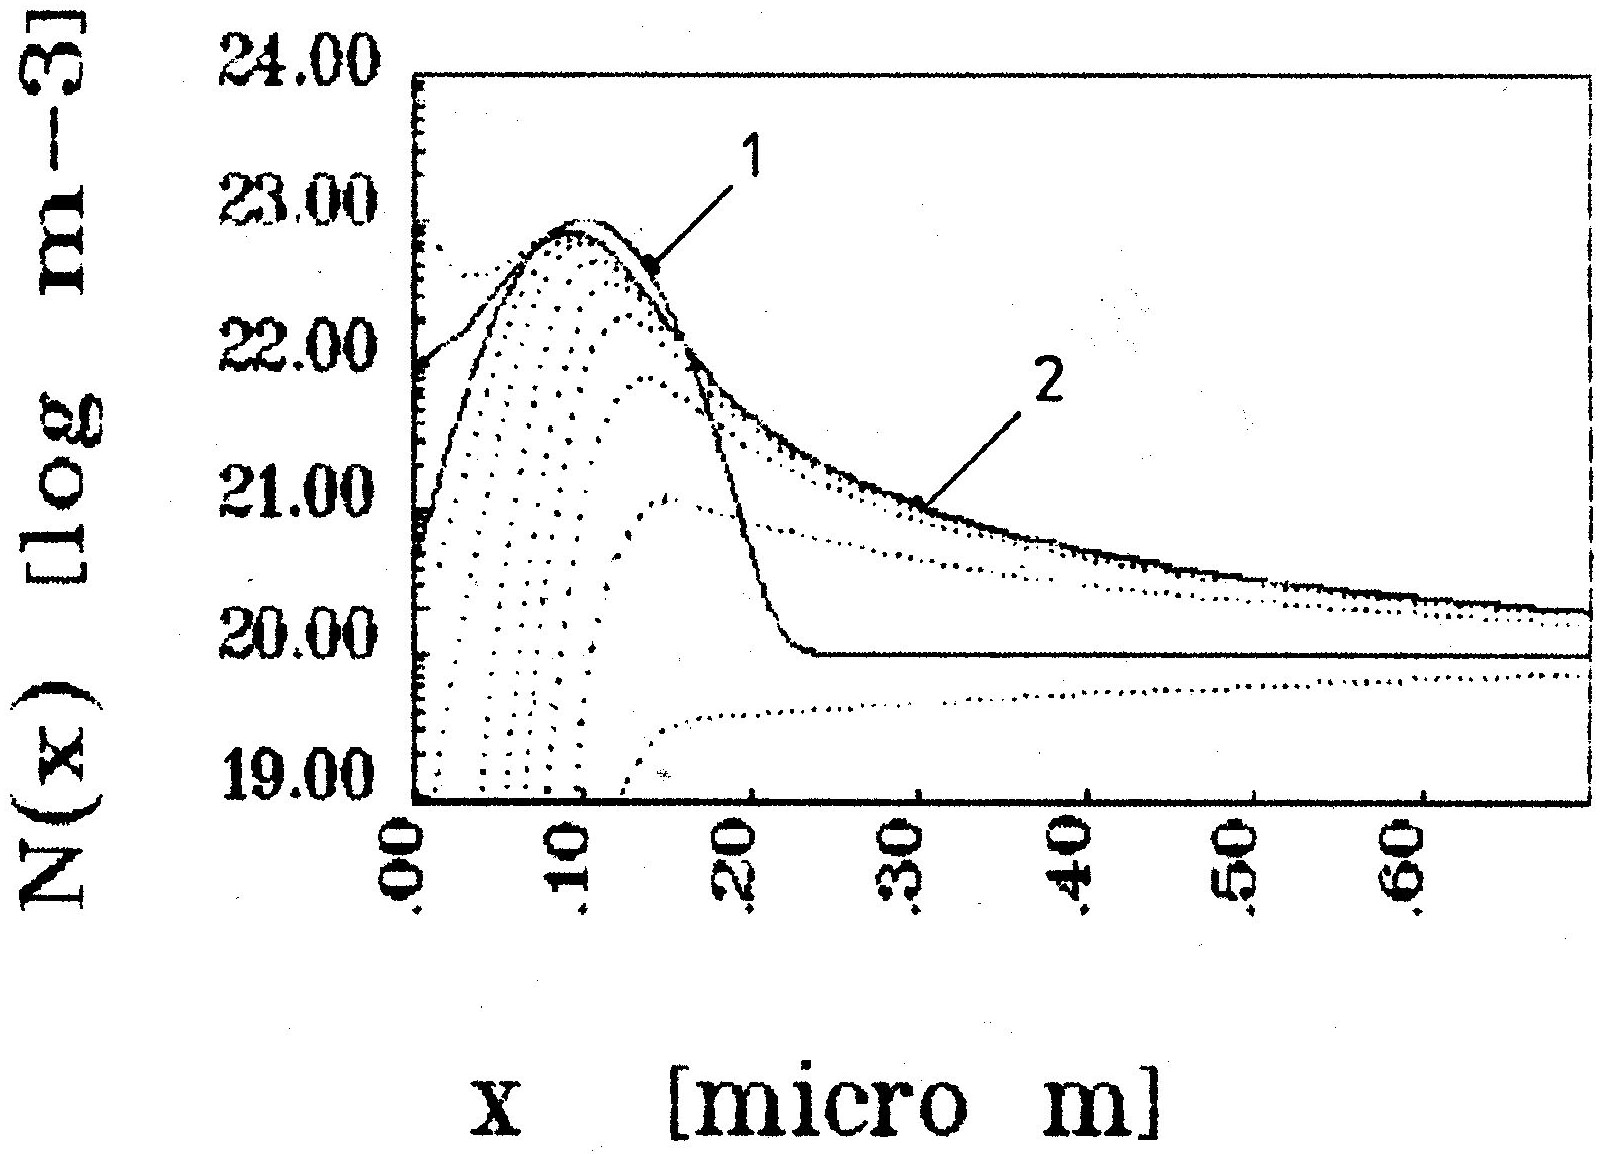
\includegraphics{Figures/fig-1-1.eps}
\captionsetup{justification=raggedright, singlelinecheck=false}
\iffalse
\caption[Priebeh koncentrácie prímesí v podpovrchovej oblasti
  polovodiča]{Priebeh koncentrácie prímesí v podpovrchovej oblasti
  polovodiča simulovaný Gaussovským rozložením \cite{1.11} s
  následovnými parametrami $R_p=0.1 \mu{m}$; $\Delta{R_p}=0.03
  \mu{m}$; $N_{max}=10^{23} m^{-3}$; $N_{bulk}=10^{20} m^{-3}$
  (označený plnou čiarou 1). Priebeh majoritných nosičov náboja pre
  $V_g=0$ (označený plnou čiarou 2). Bodkovanými čiarami sú znázornené
  priebehy koncentrácií majoritných nosičov pre napätia hradla rôzne
  od nuly. Stav termodynamickej rovnováhy medzi rozložením prímesí a
  nosičov náboja je popísaný v dodatku \ref{app:AppendixD}.}
\fi
\caption[Concentration of dopant in the subsurface of the
  semiconductor] {Concentration of dopant in the subsurface of the
  semiconductor simulated by Gaussian distribution \cite{1.11} with
  the following parameters $R_p=0.1 \mu{m}$; $\Delta{R_p}=0.03\mu{m}$;
  $N_{max}=10^{23} m^{-3}$; $N_{bulk}=10^{20} m^{-3}$ (indicated by a
  solid line 1). The profile of the majority charge carriers for
  $V_g=0$ (indicated by a solid line 2). The dotted line shows
  profiles of the concentrations of majority carriers for various gate
  voltages different from zero. State of thermodynamic equilibrium
  between the distribution of dopant and charge carriers is described
  in Appendix \ref{app:AppendixD}.}
\label{fig:1.1}
\end{figure}

\iffalse
\par Na obrázku \ref{fig:1.1} je znázornený priebeh koncentrácie
prímesí v polovodiči (simulovaný Gaussovským priebehom) a priebehy
majoritných nosičov náboja pre stav štruktúry meniaci sa od obohatenia
do inverzie, znázorňujúce dej ochudobňovania podpovrchovej oblasti
polovodiča. Tu vidieť, že priebeh koncentrácie majoritných nosičov v
implantovanej oblasti nadobúda maximum a potom klesá ku koncentrácii
substrátu, ktorú dosiahne v bode nulového elektrického potenciálu.
Zároveň je zrejmý rozdiel medzi priebehom koncentrácie prímesí a
priebehom koncentrácie majoritných nosičov náboja v stave
termodynamickej rovnováhy pre nulové napätie hradla, ktorý vzniká v
dôsledku difúzie majoritných nosičov náboja.
\fi
\par Figure \ref{fig:1.1} shows the profile of the dopant
concentration in semiconductor (simulated by Gaussian function) and
profiles of majority charge carriers for states of the structure
varying from enrichment to inversion, depicting the process of
depletion of the semiconductor subsurface. It can be seen, that the
profile of the concentration of majority carriers in implanted field
enter the maximum and then decreases toward the concentration of the
substrate, which is reached at a ground potential point. Also obvious
is the difference between the concentrations of dopant and the
concentration of majority charge carriers in the state of
thermodynamic equilibrium for zero gate voltage, which results indue
to diffusion of majority charge carriers.

\begin{figure}[h!]\centering
%\framebox[10cm]{\rule{0cm}{3cm}}
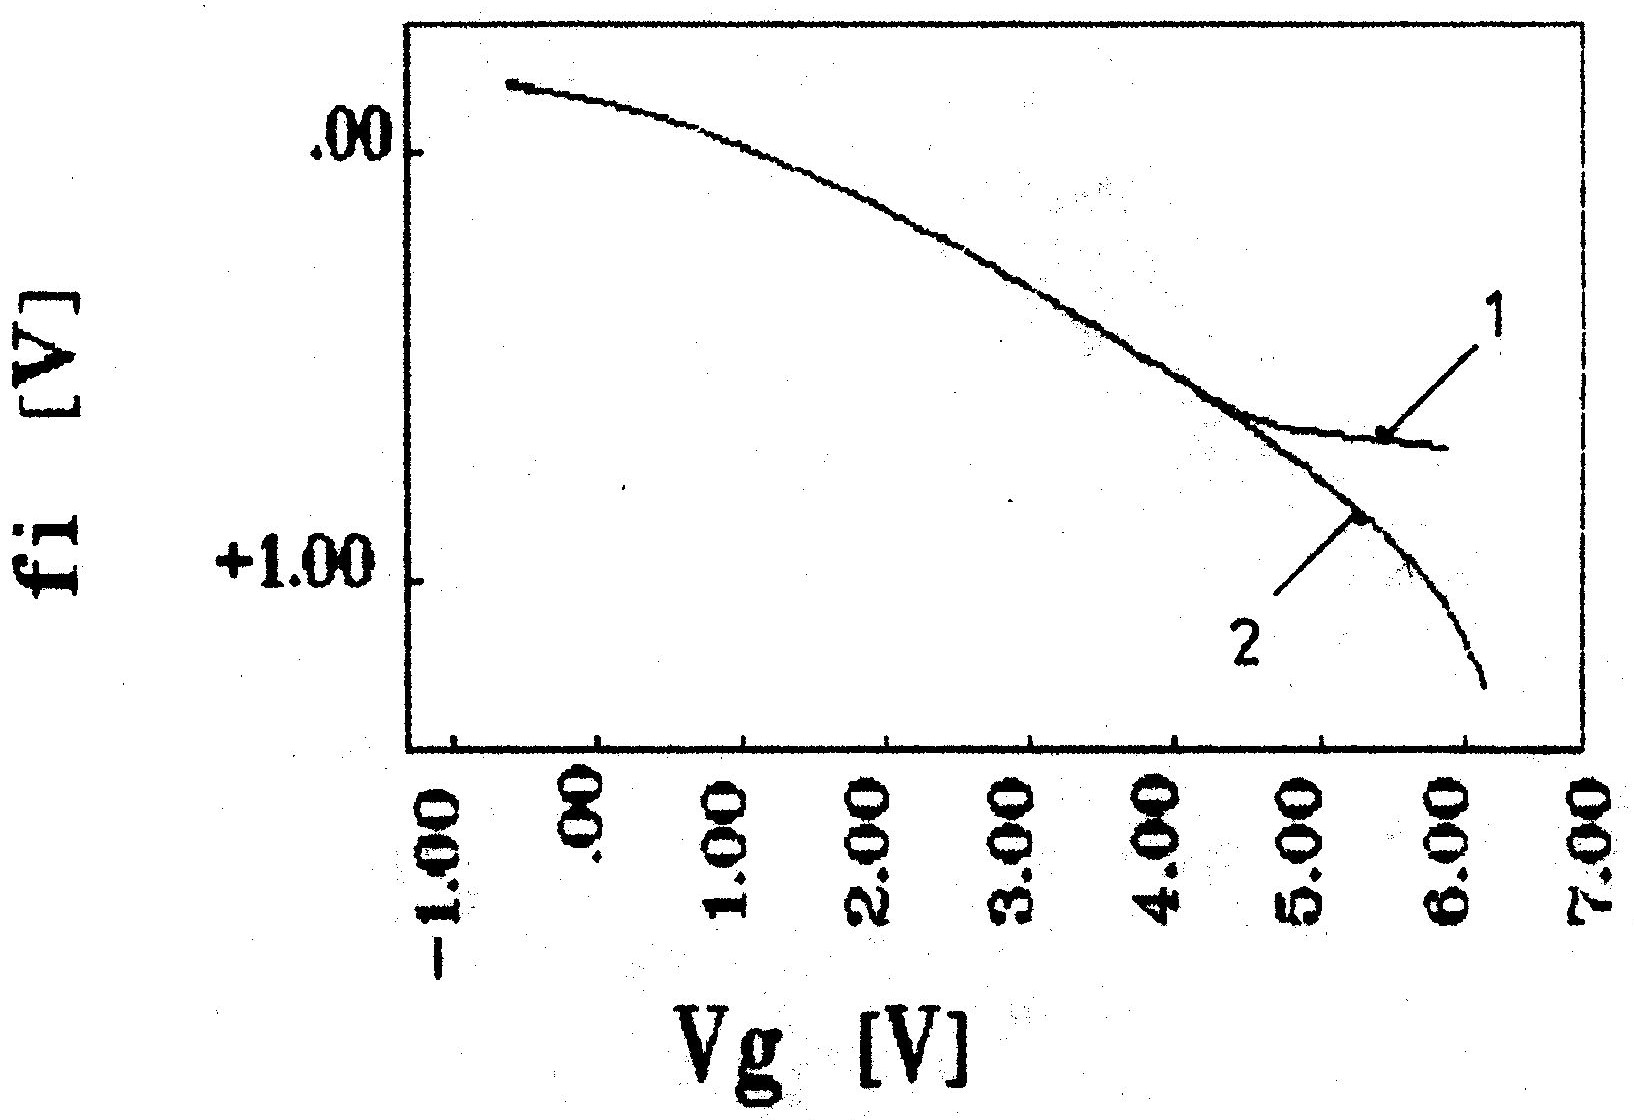
\includegraphics{Figures/fig-1-2.eps}
\captionsetup{justification=raggedright, singlelinecheck=false}
\iffalse
\caption[Priebeh povrchového potenciálu $\varphi_s(V_g)$ ako funkcie
  napätia hradla]{Priebeh povrchového potenciálu $\varphi_s(V_g)$ ako
  funkcie napätia hradla pre nízkofrekvenčné (LF) a vysokofrekvenčné
  (HF) meranie (označený 1) a pre meranie v stave hlbokého
  ochudobnenia (označený 2).}
\fi
\caption[Surface potential $\varphi_s(V_g)$ as a function of the gate
  voltage]{Surface potential $\varphi_s(V_g)$ as a function of the
  gate voltage for low frequency (LF) and high frequency (HF)
  measurement (depicted 1) and measurement in deep depletion (depicted
  2).}
\label{fig:1.2}
\end{figure}

\iffalse \par Na obrázku \ref{fig:1.2} sú znázornené priebehy
povrchového potenciálu pre rôzne režimy merania štruktúry MOS. V
oblasti obohatenia a ochudobnenia sú obidva priebehy rovnaké. Od
počiatku inverzie sa povrchový potenciál pre LF a HF meranie ustaľuje
v dôsledku vytvárania inverznej vrstvy.  Krivka hlbokého ochudobnenia
ďalej klesá. Tento stav sa v reálnej štruktúre ukončí elektrickým
prierazom.
\fi

\par Figure \ref{fig:1.2} shows surface potential for various
measurements of the MOS structure. In the enhancement and depletion
both curves are identical. From the beginning of the inversion the
surface potential stabilizes for LF and HF measurements as a result of
the creation of the inversion layer. The curve of deep depletion
further declines. This state will be terminated by the breakdown in a
real structure.

\iffalse
\par Na obrázku \ref{fig:1.3} sú znázornené kapacitne-napäťové
závislosti štruktúry MOS. Všetky tri krivky majú spoločný priebeh v
oblasti obohatenia a ochudobnenia (spoločný priebeh majú aj krivky
povrchového potenciálu). V tejto časti klesá kapacita pomaly, pretože
oblasť priestorového náboja sa rozpína cez oblasť s vysokou
koncentráciou prímesí (obr.1.1). Od počiatku inverzie sa krivky
rozdeľujú. Nízkofrekvenčná krivka, ktorá zaznamenáva inverznú vrstvu,
stúpa až ku kapacite oxidu. Vysokofrekvenčná krivka nezaznamenáva
inverznú vrstvu, pretože minoritné nosiče nestačia sledovať
vysokofrekvenčný merací signál, avšak kapacita už ďalej neklesá,
pretože so zvyšovaním napätia hradla sa zvyšuje prevážne koncentrácia
minoritných nosičov v inverznej vrstve a oblasť priestorového náboja
sa ďalej nerozpína.
\fi
\par Figure \ref{fig:1.3} shows Capacitance-Voltage profiles of the
MOS structure. All three curves are identical in enhancement and
depletion (profiles of the surface potential are also identical). In
this section the capacity declines slowly, because the space charge
region expands to the region with high concentration of the dopant
\ref{fig:1.1}. From the beginning of the inversion the the curves
depart. Low frequency curve, which detects the inversion layer rises
toward the capacity of the silica. High frequency curve doesn't detect
the inversion layer, because the minority charge carriers are not able
to follow the high frequency measurement signal. However the capacity
doesn't decline any further, because with the increasing of the gate
voltage increases mostly the concentration of the minority charge
carriers in the inversion layer and the space charge region doesn't
expand any further.

\begin{figure}[h!]\centering
%\framebox[10cm]{\rule{0cm}{3cm}}
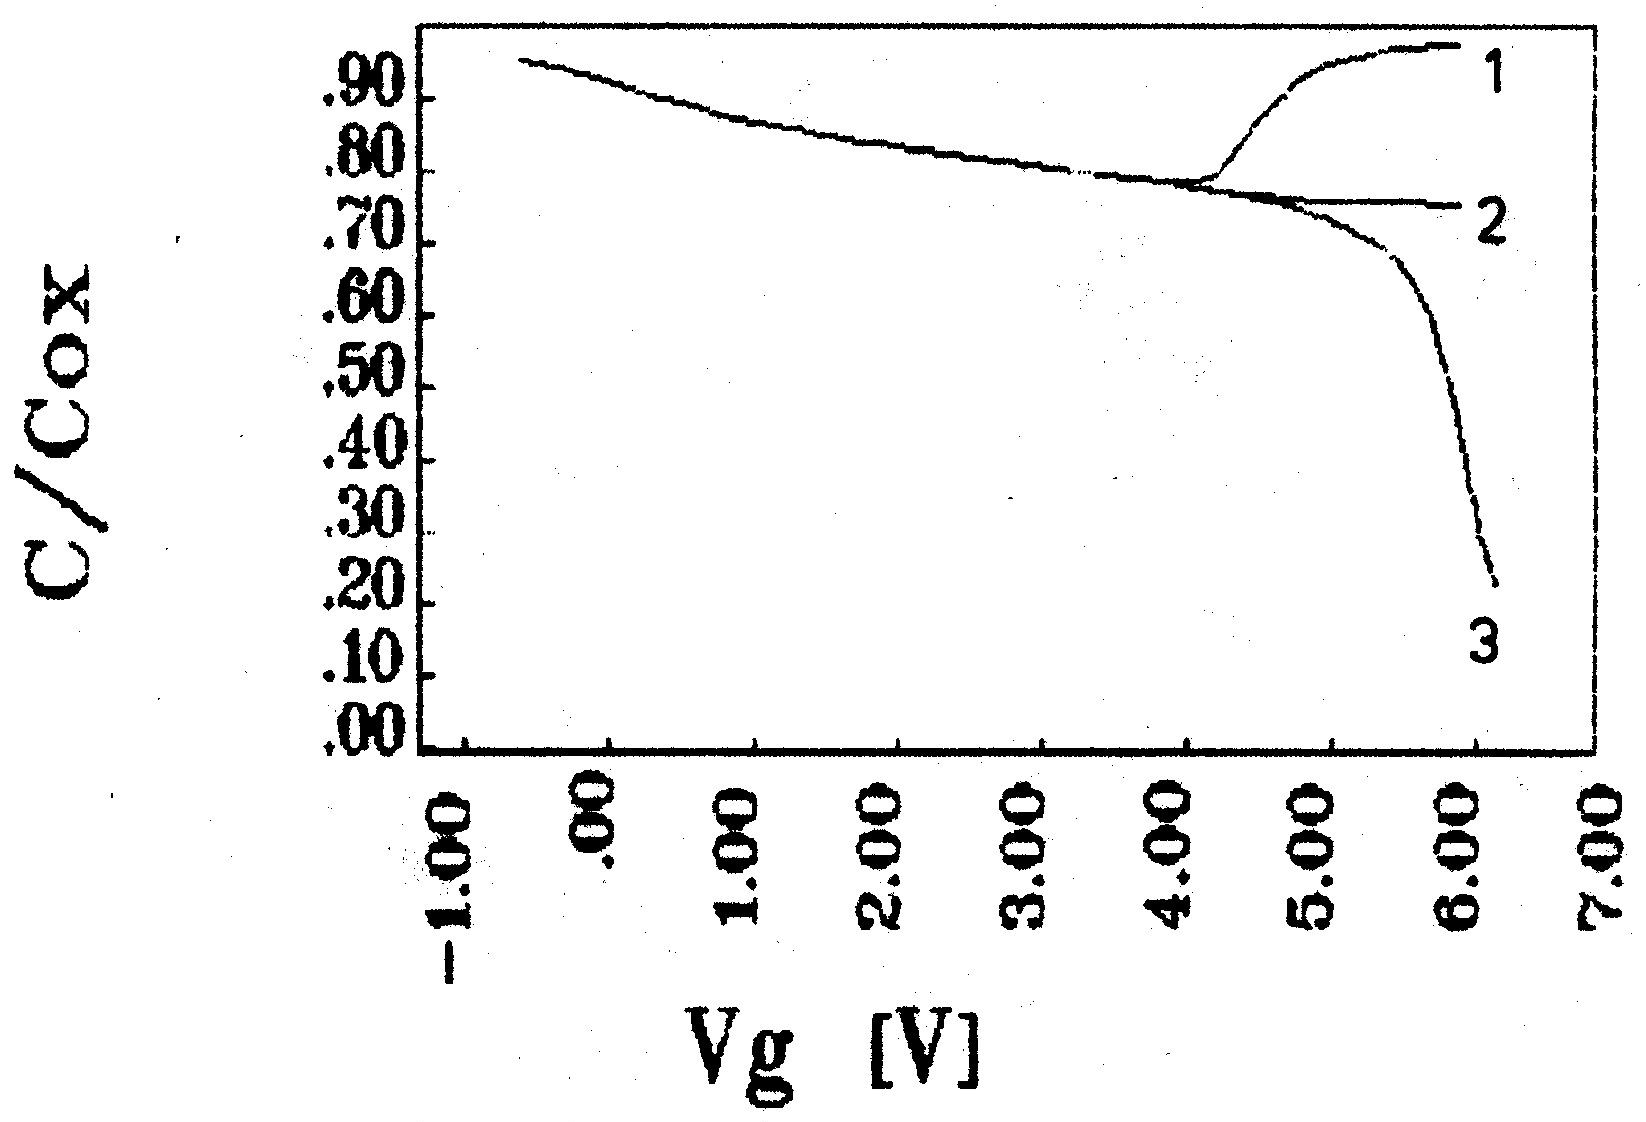
\includegraphics{Figures/fig-1-3.eps}
\captionsetup{justification=raggedright, singlelinecheck=false}
\iffalse
\caption[Priebeh kapacity štruktúry MOS v závislosti od napätia
  hradla]{Priebeh kapacity štruktúry MOS v závislosti od napätia
  hradla pre nízkofrekvenčné meranie (označené 1), vysokofrekvenčné
  meranie (označené 2) a meranie v stave hlbokého ochudobnenia
  (označené 3).}
\fi
\caption[Profile of the capacity of the MOS structure depending on the
  gate voltage]{Profile of the capacity of the MOS structure depending
  on the gate voltage for low frequency measurement (depicted 1), high
  frequency measurement (depicted 2) and measurement in deep depletion
  (depicted 3).}
\label{fig:1.3}
\end{figure}

\iffalse
\par V stave hlbokého ochudobnenia sa nevytvára inverzná vrstva a so
zvyšovaním napätia hradla sa oblasť priestorového náboja naďalej
rozpína a kapacita klesá. Z obrázku \ref{fig:1.3} je vidieť, že po
prekonaní oblasti s vysokou koncentráciou prímesí krivka hlbokého
ochudobnenia začína klesať rýchlejšie.
\fi
\par No inversion layer is created in deep depletion and with the
increasing gate voltage the space charge region expands and capacity
declines. Figure \ref{fig:1.3} shows, that after having passed the
section with the high concentration of dopant the curve of deep
depletion starts to decline faster.

\iffalse
\section{Reálna štruktúra MOS.}  Odlišnosť ideálnej a reálnej
štruktúry MOS bola obsažne spracovaná v práci \cite{1.12} a tu
uvedieme len prehľad tejto problematiky. Elektrické vlastnosti reálnej
štruktúry MOS sa líšia od ideálneho modelu hlavne vplyvom poruchových
nábojov v oxidovej vrstve a na jej rozhraní s polovodičom a kovom,
ktoré možno rozdeliť do nasledovných skupín:
\fi
\section{Real MOS structure.}
The difference of ideal and real MOS structure was treated in
\cite{1.12} and here we introduce only a review. Electrical properties
of real MOS structure are different from the ideal model mainly due to
the defect charges in the oxide layer and in its interface with the
semiconductor and metal, which can be divided into the following
groups:

\iffalse
\begin{itemize}
\item náboj pohyblivých iónov vo vrstve oxidu - $Q_{m}$
\item náboj ionizovaných pascí v oxide - $Q_{ox}$
\item fixný náboj na rozhraní $Si-SiO_2$ , spôsobený nestechiometrickým
  zložením v oblasti fázového prechodu - $Q_f$
\item náboj pascí na rozhraní $Si-SiO_2$  - $Q_{it}$
\end{itemize}
\fi
\begin{itemize}
\item charge of the mobile ions in the oxide layer - $Q_{m}$
\item charge of the ionized traps in the oxide - $Q_{ox}$
\item fixed charge at the interface $Si-SiO_2$, due to the
  non-stoichiometric composition of the phase transition - $Q_f$
\item charge of the traps at the interface $Si-SiO_2$  - $Q_{it}$
\end{itemize}

\iffalse
\par Zároveň na elektrické vlastnosti štruktúry MOS vplýva aj rozdiel
výstupných potenciálov elektrónov z kovu a polovodiča,
$\varphi_{ms}\neq{0}$. Okrem uvedených poruchových nábojov na
elektrické vlastnosti štruktúry MOS vplývajú aj geometrické
nedokonalosti štruktúry, ako aj zmena hrúbky izolačnej vrstvy a
nerovinnosť plochy rozhrania $Si-SiO_2$ . Pri prechode k veľmi veľkej
integrácii vznikla potreba zaoberať sa aj mikrodefektami v objeme
kremíka, ktoré predstavujú poruchy kryštalickej mriežky pri výrobe
monokryštálu, jeho primárnom spracovaní do formy kremíkového plátku a
v priebehu technologického spracovania súčiastky. Ak sa uvedené
defekty nachádzajú vo funkčnej oblasti súčiastky, majú nepriaznivé
účinky na elektrické parametre, avšak v objeme polovodiča mikrodefekty
vhodných veľkostí spôsobujú getračné efekty, čo sa často využíva na
tvorbu tzv. denudovanej zóny.  Zámerným vytváraním mikrodefektov v
objeme polovodiča pomocou implantácie uhlíka a následným tepelným
spracovaním možno napríklad podstatne zvýšiť dobu života minoritných
nosičov náboja \cite{1.13}. V práci \cite{1.14} autori zreteľne
zobrazili pomocou laserovej rastrovacej tomografie denudovanú zónu pri
povrchu kremíka, vytvorenú getračnými efektami mikroprecipitátov
$SiO_x$. Zároveň je z obrázkov vidieť mikroprecipitáty v objeme
polovodiča, vytvorené pomocou kyslíka a patričného tepelného
spracovania.
\fi

\par At the same time the electrical properties of MOS structure are
also affected by the difference in work function between metal and
semiconductor, $\varphi_{ms}\neq{0}$. In addition to the defect
charges geometrical imperfections of the structure, changing thickness
of the insulating layer and non-planarity of the interface $Si-SiO_2$
influence electrical properties of MOS structure. The transition to a
very large integration requires to address the micro-defects in the
volume of silicon, which represent a disorder of the crystal lattice
resulted in the production of the mono-crystal, its primary treatment
to the form of a silicon wafer and during the technological processing
of the components. If those defects are found in the area of
functional parts, they have adverse effects on electrical
parameters. However, micro-defects of suitable size in the volume of
semiconductor produce effects which are often used to create so-called
denuded zone. Deliberate creation of micro-defects in the volume of
semiconductor by implantation of carbon and subsequent heating may
significantly increase the lifetime of the minority charge carriers
\cite{1.13}. In \cite{1.14} authors clearly displayed with laser
scanning tomography a denuded zone at silicon surface formed by
microprecipitates $SiO_x$. Microprecipitates in the volume of the
semiconductor, created with oxygen and appropriate heat-processing,
are also seen from the images.

\begin{thebibliography}{}
\bibitem[1.1]{1.1} Csabay O. et al: Výskum štruktúr MIS a
  pasivácie. Záverečná správa štátnej výskumnej úlohy III-4-3/2. EF
  SVŠT, Bratislava 1980.
\bibitem[1.2]{1.2} Csabay O. et al: Výskum elektrofyzikálnych
  vlastností mikroelektronických unipolárnych štruktúr. Záverečná
  správa štátnej výskumnej úlohy III-6-1/13. EF SVŠT, Bratislava 1985.
\bibitem[1.3]{1.3} Csabay O., Botka V. et al: Elektrofyzikálne
  vlastnosti mikroelektronických štruktúr. Priebežná správa Štátnej
  výskumnej úlohy III-7-2/04. Katedra mikroelektroniky EF SVŠT,
  Bratislava 1988.
\bibitem[1.4]{1.4} Csabay O., Botka V. et al: Elektrofyzikálne
  vlastnosti mikroelektronických štruktúr. Záverečná správa Štátnej
  výskumnej úlohy III-7-2/04, Katedra mikroelektroniky EF SVŠT,
  Bratislava 1990.
\bibitem[1.5]{1.5} Žiska M.: Kandidátska dizertačná práca. Katedra
  mikroelektroniky EF SVŠT, Bratislava 1985.
\bibitem[1.6]{1.6} Harmatha L.: Výskum vlastností štruktúry MIS v
  nerovnovážnom stave kapacitnou metódou. Kandidátska dizertačná
  práca. Katedra mikroelektroniky EF SVŠT, Bratislava 1983.
\bibitem[1.7]{1.7} Valehrachová D.: Kandidátska dizertačná
  práca. Katedra mikroelektroniky EF SVŠT, Bratislava
\bibitem[1.8]{1.8} Kinder R.: Príspevok ku skúmaniu koncentračných
  profilov implantovaných vrstiev. Kandidátska dizertačná práca. EF
  SVŠT Bratislava 1984.
\bibitem[1.9]{1.9}
  \href {http://ieeexplore.ieee.org/xpl/articleDetails.jsp?arnumber=4236397&filter\%3DAND\%28p_IS_Number\%3A4236383\%29}
    {El- Sissi H., Cobbold R.S.C.: Electronic Letters 25 (1973) s.594.}
\bibitem[1.10]{1.10} 
  \href {http://ieeexplore.ieee.org/xpl/freeabs_all.jsp?arnumber=1477966}
        {Klopfenstein R.W., Wu C.P.: IEEE Trans. on electron. devices}
        ED-22 (1975) s.329.
\bibitem[1.11]{1.11}
  \href {http://www.springer.com/us/book/9783519032069}
  {Ryssel H., Ruge I.: Ionenimplantation. Stuttgart 1978}
\bibitem[1.12]{1.12} Csabay O.: Niektoré technologické a fyzikálne
  problémy štruktúr MIS. Doktorská dizertačná práca. Katedra
  mikroelektroniky, EF SVŠT, Bratislava 1986.
\bibitem[1.13]{1.13}
  \href {http://ieeexplore.ieee.org/xpl/articleDetails.jsp?arnumber=59491&filter\%3DAND\%28p_IS_Number\%3A2166\%29\%26pageNumber\%3D2}
    {Skorupa W., Kogler R. : Electronics Letters Vol.25 (1989) s.1898.}
\bibitem[1.14]{1.14}
  \href {http://ieeexplore.ieee.org/xpl/login.jsp?tp=&arnumber=18492&url=http\%3A\%2F\%2Fieeexplore.ieee.org\%2Fxpls\%2Fabs_all.jsp\%3Farnumber\%3D18492}
    {Gall P. at al. : Electronics Letters Vol.25 (1989) s.429.}
\end{thebibliography}

% Chapter 2

\chapter{Objectives of the dissertation.}\label{Chapter2}
\lhead{Chapter 2. \emph{Dissertation Objectives}}
%- - - - - - - - - - - - - - - - - - - - - - - - - - - - - - - - - - -

\begin{enumerate}
\item Building an automated experimental facility for analysis of
  electrophysical properties of MOS structures with inhomogeneous
  distribution of dopants in the substrate, with the ability to
  monitor area distribution of the investigated parameters on the
  silicon substrate.  The workstation includes a high-frequency C-V
  method (including depleted C-V method), low-frequency C-V method,
  low-frequency constant width OPN (CCT) and Q-C method.
\item Automate the methods referred to in point 1.  PC AT computer
  under MS DOS operating system.  To implement methods to use the GPIB
  PCIIA interface, HP4280a measuring instruments, Keithley 642 and a
  Zond A5 tip stepper.
\item The implemented methods are used to determine the depth
  concentration profiles of implanted impurities, oxide layer
  thickness, stress of aligned bands, trap density of the Si-SiO
  interface and depth generation lifetime profile of minority charge
  carriers.  Analyse the problems arising in determining the
  parameters of MOS structures in conjunction with inhomogeneous
  substrate endowment.
\item Determine the depth concentration profiles of active impurities
  and their distributions on the silicon substrate for different
  implantation doses in ranging from $0.6\times{10}^{15}$ to
  $60.0\times{10}^{15}{m}^{-2}$. To investigate how implantation dose
  affects the properties of the Si-SiO interface and the depth
  lifetime profile of minority charge carriers.  Propose a methodology
  for identifying the amount of implanted ions in a semiconductor
  substrate using a capacitive method.
\end{enumerate}

% Chapter 3

\chapter{Použité metódy merania štruktúry MOS.} % Main chapter title

\label{Chapter3} % For referencing the chapter elsewhere, use \ref{Chapter1} 

\lhead{Chapter 3. \emph{Použité metódy merania štruktúry MOS}} % This is for the header on each page - perhaps a shortened title

%----------------------------------------------------------------------------------------

Kapacitne-napäťové (C-V) metódy, ktorými sa v tejto práci budeme
zaoberať, poskytujú komplexné informácie o elektro-fyzikálnych
parametroch štruktúry MOS.  Pre určenie niektorých parametrov
postačuje vyhodnotenie dát nameraných pomocou jednej metódy, no vo
väčšine prípadov kombináciou viacerých metód možno získať presnejšie
výsledky.  V predchádzajúcej kapitole sme na príklade výpočtu C-V
závislosti ideálnej štruktúry MOS demonštrovali rozdiely medzi
napäťovými závislosťami kapacity štruktúry MOS, meranými rozličnými
metódami:

\begin{itemize}
\item nízkofrekvenčnou (prípadne kvázistatickou) C-V metódou
\item rovnovážnou vysokofrekvenčnou C-V metódou
\item nerovnovážnou vysokofrekvenčnou C-V metódou.
\end{itemize}

Okrem uvedených metód sme v dizertačnej práci použili Q-C metódu,
ktorá kombinuje vlastnosti vysokofrekvenčnej a nízkofrekvenčnej C-V
metódy. Určenie tých istých C-V závislostí pomocou rôznych metód
zároveň predstavuje určitý druh kontroly presnosti merania.  To je
výhodné hlavne v prípadoch, kedy určenie absolútnej chyby merania
predstavuje komplexný problém. Pre meranie generačného času života
minoritných nosičov náboja sme použili metódu konštantnej šírky OPN
\cite{3.1}, ktorej výhodou oproti klasickej Zerbstovej C-t metóde
\cite{3.2} je väčšia rýchlosť merania. Modifikácia metódy konštantnej
šírky OPN \cite{3.3} zároveň eliminuje vplyv bočnej injekcie
minoritných nosičov náboja do OPN zo substrátu.

Výhodou uvedených metód je, že nie su deštruktívne, čo ich v spojení s
ich rýchlosťou predurčuje pre rutinné použitie v priemysle.  V
laboratórnych podmienkach je vhodné tieto metódy overiť pomocou
ďalších metód, ktoré možno považovať za doplnkové. Tak je tomu pri
meraní koncentračného profilu prímesí, napríklad metódou rozptylového
odporu, elektrochemickou kapacitnou metódou, prípadne SIMS. Vhodné je
aj overenie koncentračného profilu pomocou simulácie technologického
procesu. Pri skúmaní energetických stavov nachádzajúcich sa v
zakázanom pásme polovodiča, kvalitné informácie poskytuje metóda DLTS.

Uvedené C-V metódy predstavujú podmnožinu širokej oblasti diagnostiky
štruktúr MOS pomocou kapacitných meraní.  Následujúca schéma
znázorňuje ich vztah ku skúmaným parametrom, ktoré boli predmetom
tejto práce a zároveň poukazuje na okruhy problémov, ktoré bolo
potrebné riešiť.

% start with Fig3.0 to preserve the numbering in the original
% publication
%\setcounter{figure}{0}
%\addtocounter{figure}{-1}
%\begin{figure}[h!]\centering
%\framebox[10cm]{\rule{0cm}{3cm}}
%\caption{Schéma vzťahu C-V metód a skúmaných parametrov}
\begin{diagram}
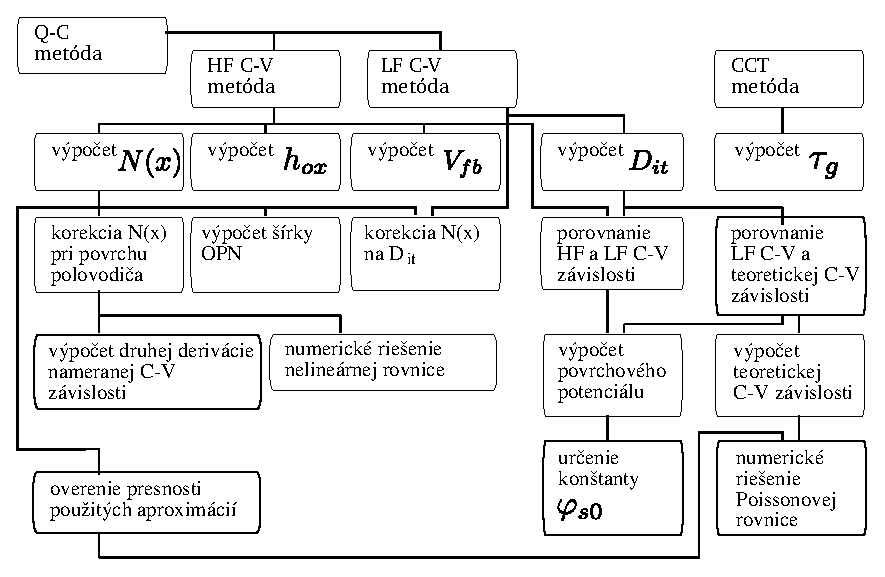
\includegraphics[width=\textwidth,height=\textheight,scale=0.7,keepaspectratio]{Figures/diagram-1.EPS}
\label{diagram:1}
\end{diagram}


\section{Vysokofrekvenčná C-V metóda.}\label{sec:3.1}

Pri meraní vysokofrekvenčnou kapacitnou metódou je MOS štruktúra
jednosmerným hradlovým napätím privedená do požadovaného stavu a jej
kapacita sa určí z prúdovej odozvy na vysokofrekvenčný signál malej
amplitúdy, ktorý je nasuperponovaný na jednosmerné hradlove
napätie. Meraním fázového posuvu medzi vysokofrekvenčným napäťovým
signálom a prúdom možno okrem kapacity zároveň vyhodnotiť aj vodivosť
štruktúry. Veľkost frekvencie meracieho signálu je daná kompromisom
medzi požiadavkou čo najvyššej frekvencie zo strany ovplyvnenia
merania rýchlymi pascami rozhrania $Si-SiO_2$ a technickými možnosťami
štandardných meracích prístrojov.  V našom experimente sme použili
prístroj HP4280a, ktorého merací signál má pevne stanovenú frekvenciu
1 MHz a veľkost amplitúdy meracieho signálu možno voliť 10 mV, alebo
30 mV.  Spomenutý prístroj možno riadiť pomocou zbernice IMS-2. Treba
uviesť, že prístroj v spojení s riadiacim pocitacom PC AT je schopný v
blokovom prenose zmerať a v binárnom formáte preniesť do riadiaceho
počítača 680 bodov (čo je limit pre blokový prenos) C-V a G-V
závislosti za 25 sekúnd.  Uvedený časový údaj uvádzame na základe
vykonaných vlastných experimentov.

\section{Kvázistatická C-V metóda.}\label{sec:3.2}

Pri meraní kvázistatickou kapacitnou metódou je MOS štruktúra nabíjaná
pomalým, v čase narastajúcim hradlovým napätím. Kapacita MOS štruktúry
je určená ako závislosť nabíjacieho prúdu a rýchlosti nárastu
hradlového napätia.  Z uvedeného vyplýva, že na realizáciu metódy je
potrebný zdroj kontinuálne narastajúceho napätia a
ampérmeter. Rýchlosť narastania napätia musí byť dostatočne malá, aby
bola štruktúra počas merania stále v termodynamickej rovnováhe. Na
druhej strane zase so zmenšovaním rýchlosti sa zmenšuje aj prúd, ktorý
musíme merať. Pre väčšinu meraných vzoriek vyhovovala rýchlosť rádove
$10^{-2} V/s$, čo predstavuje pre kapacitu $100 pF$ nabíjací prud
$10^{-12} A$. V našom experimente sme použili na meranie prúdu
elektrometer Keithley 642, ktorý meria prúd v rozsahu od $10^{-8} A$
do $10^{-17} A$ s rozlíšením 5 číslic na rozsah.  Treba podotknúť, že
okrem iných vynikajúcich vlastností prístroja výrobca zaručuje
efektívnu hodnotu šumu menšiu ako $8$ x $10^{-17} A$. Zdroj narastajúceho
napätia, ktorý bol postavený na našej katedre, umožňuje nastavenie
rýchlosti nárastu napätia v rozsahoch od $10 V/s$ do $10^{-3} V/s$ s
rozlíšením 1\% rozsahu. Oba prístroje možno riadiť pomocou zbernice
IMS-2.  Hlavným zdrojom chýb pri kvázistatickej metóde je nepresnosť
určenia rýchlosti nárastu napätia hradla \cite{1.5}. Pred každým
meraním je potrebné presne zmerať rýchlosť nárastu napätia, ktorá sa
potom použije pri výpočte kapacity. Rýchlosť nárastu napätia pre
zvolený rozsah určujeme v našom prípade z podielu zmeny napätia a času
za 10 s.  Uvedná hodnota má potom význam strednej hodnoty a jej
použitie pri výpočte predpokladá lineárny nárast napätia, ktorý sme
experimentálne overili pre reprezentatívnu vzorku rozsahov nárastu
napätia v čase.

\section{Q-C metóda.}\label{sec:3.3}

Q-C metóda \cite{3.4} predstavuje kombináciu vysokofrekvenčnej C-V
metódy a nábojovej Q-V metódy \cite{3.5}. Jej princíp je
následovný. Do série s kondezátorom tvoreným štruktúrou MOS je
zapojená napäťovo nezávislá kapacita, ktorú označíme $C_i$ .  Na
sériovo-paralelné zapojenie kondenzátorov, ktoré je znázornené na obrázku \ref{fig:3.1}, pripojíme jednosmerné napätie $V_a$ a meriame napätie
$V_i$ v spoločnom bode zapojenia kondenzátorov, ktoré predstavujú
kapacitný delič. Kondenzátory označené $C_w$ a $C_x$ znázorňujú
parazitné kapacity. $C_w$ je kapacita medzi stolíkom a zdvihnutým
hrotom sondy a $C_x$ je kapacita spoločného bodu zapojenia
kondenzátorov voči zemi. Zároveň s meraním napätia $V_i$ zmeriame aj
kapacitu $C_m$ a vodivosť $G_m$ pomocou vysokofrekvenčného signálu
nasuperponovaného na napätí $V_a$.

\begin{figure}[h!]\centering
%\framebox[10cm]{\rule{0cm}{3cm}}
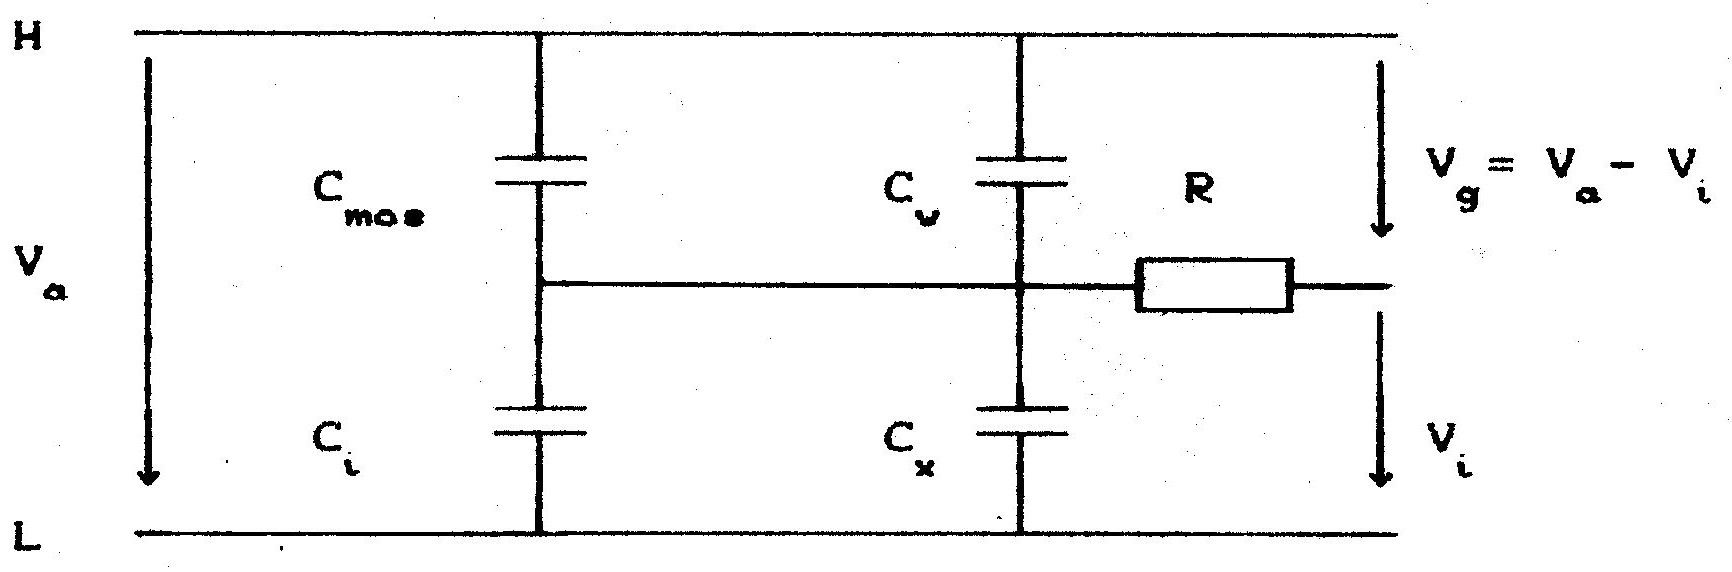
\includegraphics{Figures/fig-3-1.eps}
\captionsetup{justification=raggedright, singlelinecheck=false}
\caption[Schématické znázornenie zapojenia kondenzátorov Q-C 
metódy]{Schématické znázornenie zapojenia kondenzátorov Q-C 
metódy}
\label{fig:3.1}
\end{figure}

Medzi spoločný bod zapojenia kondenzátorov a vstup voltmetra je
pripojený odpor, ktorý spolu s kapacitou prívodných vodičov voltmetra
a vstupnou kapacitou voltmetra tvorí dolnopriepustný filter,
spôsobujúci, že merané napätie nie je ovplyvnené vysokofrekvenčným
signálom. Z uvedeného zároveň vyplýva, že veľkost kapacity medzi
spoločným bodom zapojenia a bodom L sa bude líšiť pre jednosmerné a
vysokofrekvenčné meranie. Označme preto kapacitu $C_i$ pre jednosmerné
meranie $C_{iLF}$ a pre vysokofrekvenčné meranie $C_{iHF}$.  Spomenutý
odpor spolu so vstupným odporom voltmetra tvorí napäťový delič.  Aby
tým nebolo ovplyvnené meranie napätia, treba použiť voltmeter s
vysokým vstupným odporom.  Tu treba spomenúť vhodnosť použitia
elektromeru Keithley 642, ktorého vstupný odpor v režime merania
napätia je približne $10^{16} \Omega$ a jeho parazitná vstupná
kapacita sú $2 pF$. Detailný popis zapojenia Q-C metódy, eliminácia
parazitných kapacít, prípadne metodika ich merania je popísaná v
dodatku \ref{app:AppendixE}. Ak poznáme kapacitu oxidovej vrstvy
štruktúry MOS $C_{ox}$ a veľkosť kapacity $C_{iLF}$ , môžeme vypočítať
hodnotu povrchového potenciálu $\varphi_s$ z následovného vzťahu,
odvodeného v dodatku \ref{app:AppendixF}.

\begin{equation}
\varphi_s = \varphi_{s0} + V_g ( 1 + \frac{C_w}{C_{ox}}) - V_i \frac{C_{iLF}+C_x}{C_{ox}}
\label{eq:3.1}
\end{equation}

Zároveň môžeme určiť nízkofrekvenčnú kapacitu štruktúry MOS

\begin{equation}
C^{LF}_{mos} = C_{ox} ( 1 - \frac{d\varphi_s}{dV_g})
\label{eq:3.2}
\end{equation}

Poruchové náboje nachádzajúce sa v meranej štruktúre MOS spôsobujú, že
povrchový potenciál polovodiča nadobúda hodnotu $\varphi_{s0}$ aj pri
nulovom napätí hradla. Veľkosť tejto konštanty možno určiť z
porovnania nameranej a teoretickej závislosti povrchového potenciálu
od šírky OPN $\varphi(x)$.  Metóda určenia $\varphi_{s0}$ je popísaná
v dodatku \ref{app:AppendixG}. Tu možno poznamenať, že pre výpočet
$C^{LF}_{mos}$ hodnotu tejto konštanty nepotrebujeme, ako je zrejmé zo
vzťahov \ref{eq:3.1} a \ref{eq:3.2}.

Z nameraných hodnôt $C_m$ a $G_m$ môžeme určiť vysokofrekvenčnú
kapacitu štruktúry MOS pomocou následovných vzťahov.  Najprv
vypočítame odpovedajúci odpor $R_m$ a reaktanciu $X_m$

\begin{subequations}\label{eq:3.3}
\begin{align}
R_m &= \frac{G_m}{G^2_m + (\omega C_m)^2}\label{subeq:3.3a}\\[0.5cm]
X_m &= \frac{\omega C_m}{G^2_m + (\omega C_m)^2}\label{subeq:3.3b}\\[0.5cm]
\intertext{,ktoré použijeme vo vzťahu}
C^{HF}_{mos} &= - \frac{R^2_m + (X_m + \frac{1}{\omega C_{iHF}} + \omega C_w D^2)^2}{\omega D^2(X_m + \frac{1}{\omega C_{iHF}} + \omega C_w D^2)^2}\label{subeq:3.3c}\\[0.5cm]
\intertext{,kde}
D^2 &= R^2_m + (X_m + \frac{1}{\omega C_{iHF}})^2\label{subeq:3.3d}
\end{align}
\end{subequations}

Podrobný popis a odvodenie uvedených vzťahov je popísané v dodatku
1. literatúry \cite{3.6}. Q-C metóda poskytuje celý rad výhod.
Umožňuje simultánne meranie vysokofrekvenčnej a nízkofrekvenčnej C-V
závislosti, čo zaručuje rovnaké podmienky merania pre obe závislosti a
vylučuje možnosť ich vzájomného napäťového posuvu, ktorý sa môže
objaviť ak by boli závislosti snímané sekvenčne.  Zároveň meranie
níkofrekvenčnej C-V závislosti je statické a nie je závisle od
dynamiky hradlového napätia.

Pre určenie koncentračného profilu prímesí v podpovrchovej oblasti
polovodiča je výhodné poznať priebeh povrchového potenciálu, čo
umožňuje výpočet nezaťažený pascami rozhrania $Si-SiO_2$. Uvedené
výhody sú vykompenzované náročnosťou metódy na použité prístroje.
Kritickým bodom realizácie metódy je odizolovanie spoločného bodu
zapojenia kondenzátorov. Pripojené napätie $V_a$ sa musí rozložiť na
kondenzátoroch podľa ich kapacít a nie podľa ich zvodových odporov.
To vyžaduje použitie kvalitného kondenzátora $C_i$ a usporiadanie
rozloženia jednotlivých komponentov metódy tak, aby bol zvodový prúd
zo spoločného bodu na zem čo najmenší. Tým sú z použitia Q-C metódy
vylúčené štruktúry MOS, ktoré majú veľké zvodové prúdy spôsobené
nedokonalosťou oxidovej vrstvy. Pre meranie v stave termodynamickej
rovnováhy, ako uvádzajú autori metódy \cite{3.7}, je potrebné aby sa
napätie $V_i$ nemenilo najmenej počas 10 sekúnd o veľkost rádove
$10^{-3}$ V. Pre účely určenia koncentračného profilu môžeme merať
nerovnovážnu C-V závislosť, pri ktorej sa zvodové prúdy zo spoločného
bodu na zem neprejavia v takej miere, pretože merané napätie je
odčítavané okamžite po priložení napätia. Na obrázku \ref{fig:3.2} sú
znázornené normované priebehy HF C-V závislosti štruktúry MOS a
priebehu povrchového potenciálu od napätia hradla určené pomocou Q-C
metódy pre meranie v stave termodynamickej rovnováhy a v stave
hlbokého ochudobnenia. Použité prístroje v implementácii metódy na
našom oddelení \cite{3.8,3.9} možno riadiť pomocou zbernice IMS-2 a
namerané hodnoty napätí $V_a$, $V_i$ , kapacity $C_m$ a vodivosti
$G_m$ uložiť do diskového súboru pre ďalšie spracovanie.

\begin{figure}[h!]\centering
%\framebox[10cm]{\rule{0cm}{3cm}}
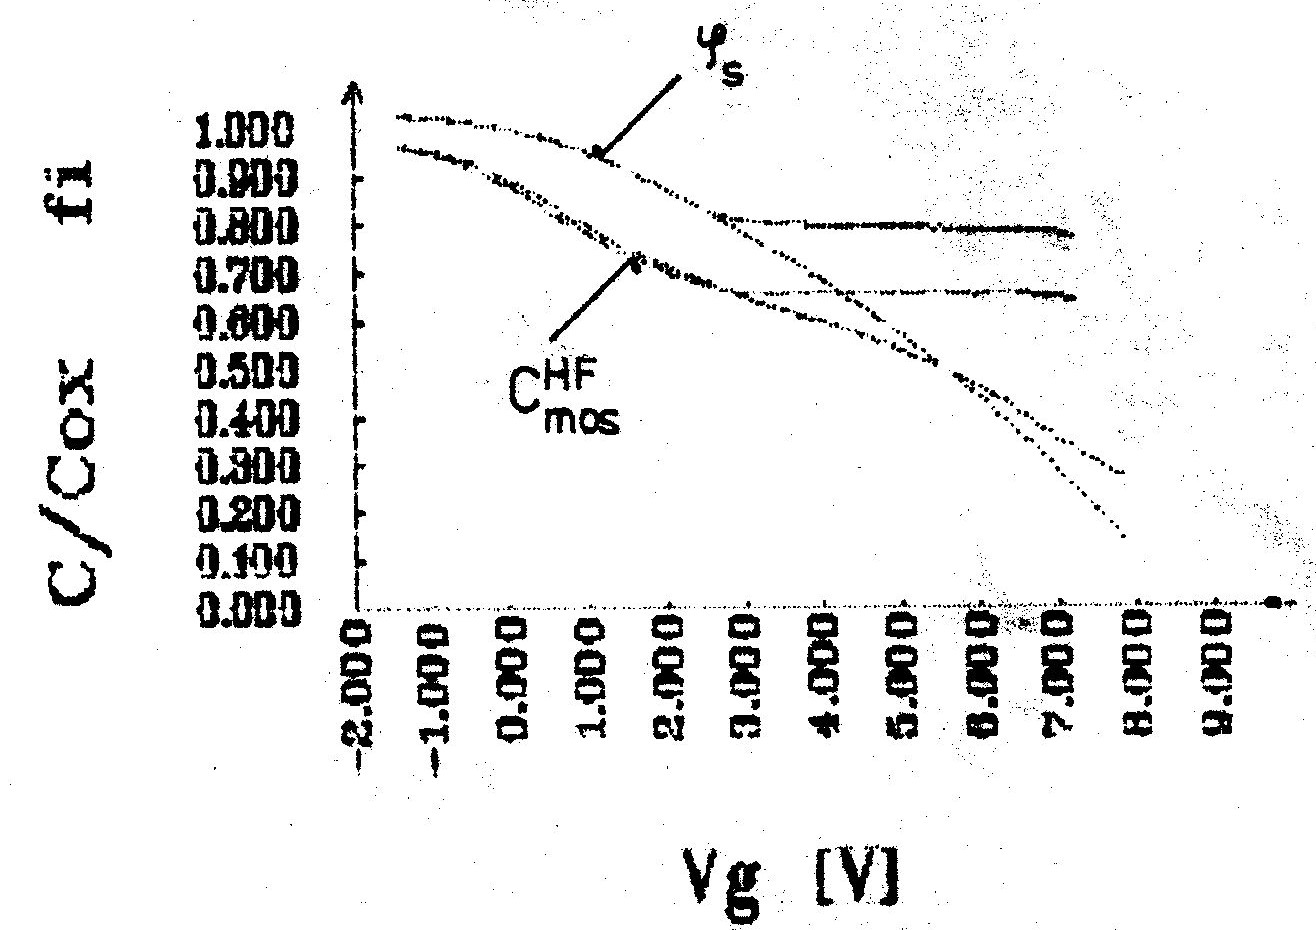
\includegraphics{Figures/fig-3-2.eps}
\captionsetup{justification=raggedright, singlelinecheck=false}
\caption[Normované priebehy HF C-V závislosti štruktúry MOS a priebehu
  povrchového potenciálu od napätia hradla určené pomocou Q-C metódy
  pre meranie v stave termodynamickej rovnováhy a v stave hlbokého
  ochudobnenia]{Normované priebehy HF C-V závislosti štruktúry
  MOS a priebehu povrchového potenciálu od napätia hradla určené
  pomocou Q-C metódy pre meranie v stave termodynamickej rovnováhy a v
  stave hlbokého ochudobnenia. Priebehy $\varphi_s(V_g)$ sú zobrazené
  s použitím normovania $1 - \frac{\varphi_s}{\varphi_{norm}}$, kde
  $\varphi_{norm}=3.33V$.}
\label{fig:3.2}
\end{figure}
%OBR7.BIT

Pre overenie presnosti Q-C metódy sme na tej istej štruktúre MOS
urobili samostatné vysokofrekvenčné a nízkofrekvenčné meranie a
zároveň vypočítali tie isté kapacitné závislosti z nameraných hodnôt
Q-C metódy.  Výsledné krivky sú na obrázkoch \ref{fig:3.3} a
\ref{fig:3.4}.

Pre kvantitatívne porovnanie výsledkov znázornených na obrázku
\ref{fig:3.3} a \ref{fig:3.4} uvádzame v tabulke \ref{tab:3.1} a
\ref{tab:3.2} číselné hodnoty normovaných kapacít $C^{HF}_{mos}$ a
$C^{LF}_{mos}$ pre metódy HF, LF a Q-C a ich rozdiel vyjadrený
relatívnou chybou. Z tabuliek vidieť rozdiel medzi jednotlivými C-V
závislosťami, čo je spôsobené jednak nepresnosťami pri určovaní
parazitných kapacít a jednak zvodovými prúdmi použitých
kondenzátorov. Autori metódy doporučujú pre elimináciu zvodových
prúdov, ktoré spôsobuje vlhkosť prostredia, použiť vzduchový
kondenzátor $C_i$ a na meranú vzorku usmerniť v priebehu merania prúd
dusíka, ktorý zabráni kondenzovaniu vodných pár z okolia.

\begin{figure}[h!]\centering
%\framebox[10cm]{\rule{0cm}{3cm}}
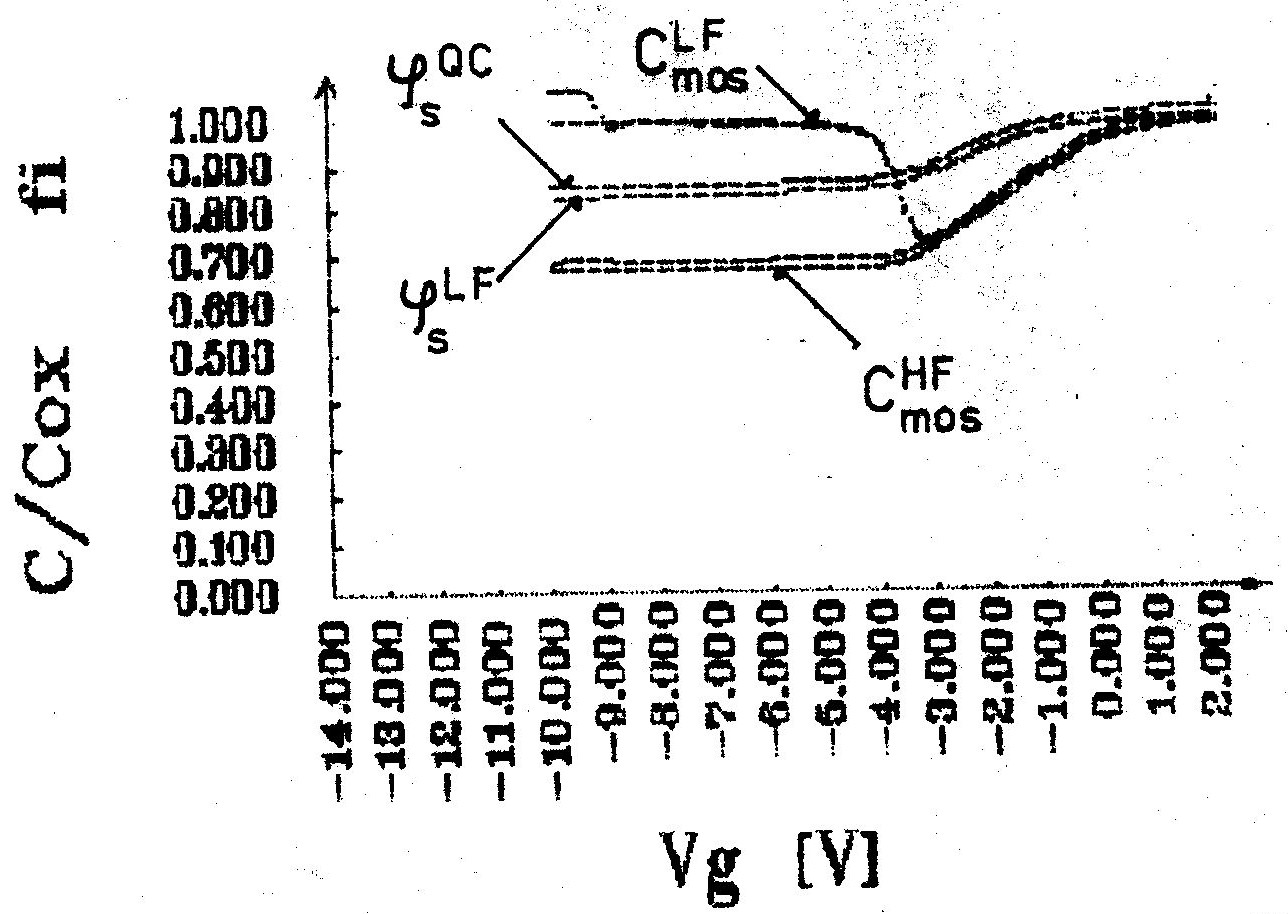
\includegraphics{Figures/fig-3-3.eps}
\captionsetup{justification=raggedright, singlelinecheck=false}
\caption[Normované priebehy kapacity štruktúry MOS so substrátom typu
  N ako funkcie napätia hradla pre rovnovážne vysokofrekvenčné a
  kvázistatické meranie]{Normované priebehy kapacity štruktúry MOS so
  substrátom typu N ako funkcie napätia hradla pre rovnovážne
  vysokofrekvenčné a kvázistatické meranie.  Zároveň sú znázornené tie
  isté charakteristiky získané pomocou Q-C metódy. Pre úplnosť je na
  obrázku znázornená závislosť povrchového potenciálu
  $\varphi_s(V_g)^{QC}$ získaná pomocou Q-C metódy a závislosť
  $\varphi_s(V_g)^{LF}$ vypočítaná integrovaním nízkofrekvenčnej C-V
  závislosti pomocou Berglundovho integrálu.  Priebehy
  $\varphi_s(V_g)$ sú zobrazené s použitím normovania $1 -
  \frac{\varphi_s}{\varphi_{norm}}$, kde $\varphi_{norm}=-3.33V$.}
\label{fig:3.3}
\end{figure}
%OBR5.BIT

\begin{figure}[h!]\centering
%\framebox[10cm]{\rule{0cm}{3cm}}
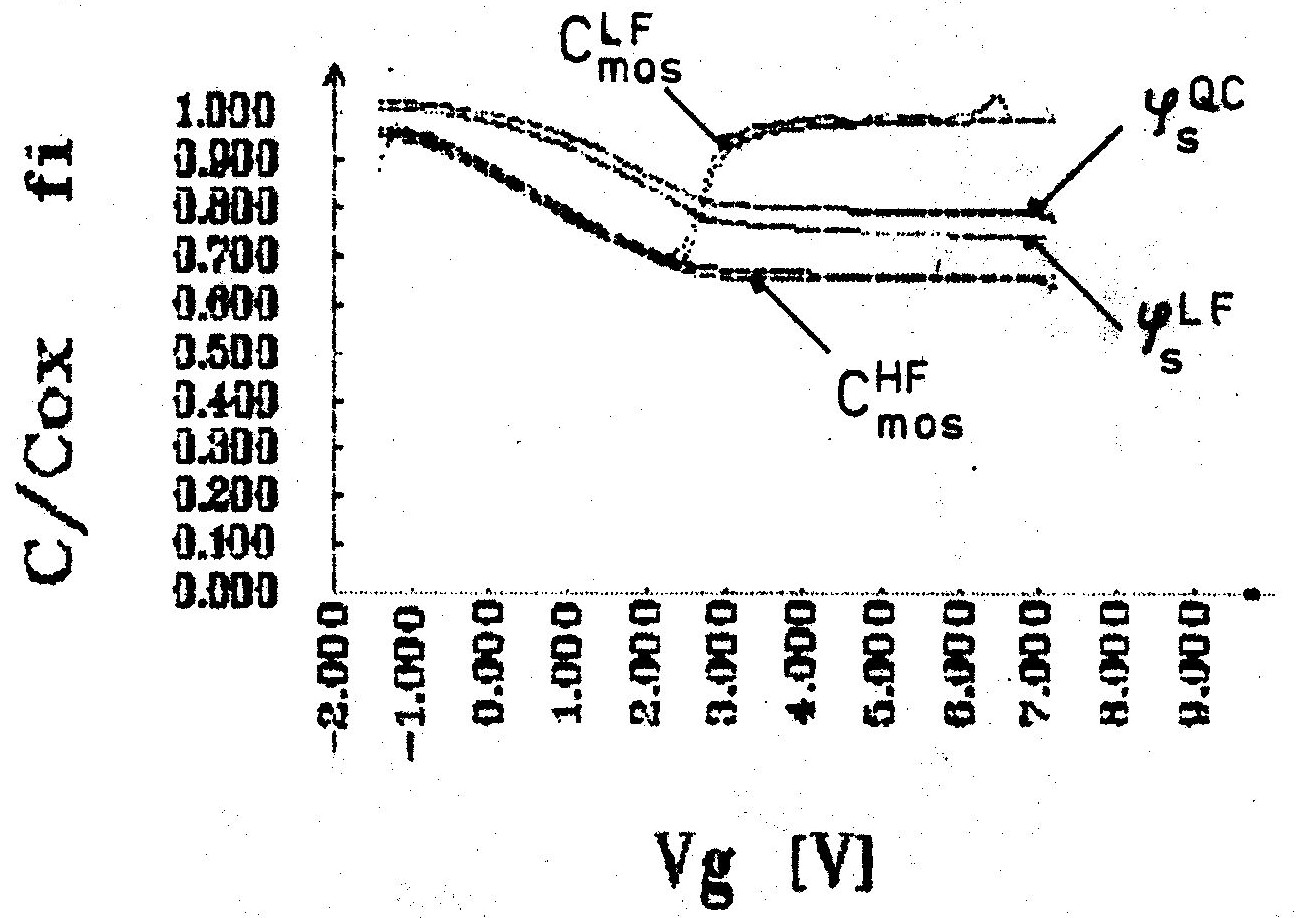
\includegraphics{Figures/fig-3-4.eps}
\captionsetup{justification=raggedright, singlelinecheck=false}
\caption[Normované priebehy kapacity štruktúry MOS so substrátom typu
  P ako funkcie napätia hradla pre rovnovážne vysokofrekvenčné a
  kvázistatické meranie]{Normované priebehy kapacity štruktúry MOS so
  substrátom typu P ako funkcie napätia hradla pre rovnovážne
  vysokofrekvenčné a kvázistatické meranie.  Zároveň sú znázornené tie
  isté charakteristiky získané pomocou Q-C metódy. Pre úplnosť je na
  obrázku znázornená závislosť povrchového potenciálu
  $\varphi_s(V_g)^{QC}$ získaná pomocou Q-C metódy a závislosť
  $\varphi_s(V_g)^{LF}$ vypočítaná integrovaním nízkofrekvenčnej C-V
  závislosti pomocou Berglundovho integrálu.  Priebehy
  $\varphi_s(V_g)$ sú zobrazené s použitím normovania $1 -
  \frac{\varphi_s}{\varphi_{norm}}$, kde $\varphi_{norm}=3.33V$.}
\label{fig:3.4}
\end{figure}
%OBR6.BIT

\begin{table}[h!]\centering
\begin{tabular}{|c|c|c||c|c|c|}
  \hline
  \multicolumn{3}{|c||}{$C^{HF}_{mos}$} & \multicolumn{3}{|c|}{$C^{LF}_{mos}$} \\
  \hline
  HF[\%] & QC[\%] & $\Delta_r$[\%] & LF[\%] & QC[\%] & $\Delta_r$[\%] \\
  \hline
  99.67 & 98.30 & +1.37 & 97.85 & 99.14 & -1.32 \\
  98.56 & 96.69 & +1.89 & 96.59 & 97.05 & -0.47 \\
  98.56 & 96.69 & +1.89 & 96.59 & 97.05 & -0.47 \\
  95.73 & 93.89 & +1.92 & 93.93 & 94.51 & -0.61 \\
  89.89 & 87.75 & +2.39 & 88.26 & 88.57 & -0.36 \\
  82.15 & 80.17 & +2.41 & 81.43 & 81.82 & -0.47 \\
  74.83 & 73.09 & +2.33 & 73.79 & 74.57 & -1.06 \\
  69.69 & 67.81 & +2.70 & 86.08 & 86.33 & -0.29 \\
  69.10 & 67.20 & +2.74 & 97.20 & 97.73 & -0.54 \\
  68.97 & 67.08 & +2.74 & 98.27 & 98.74 & -0.48 \\
  68.91 & 67.03 & +2.72 & 98.75 & 99.38 & -0.64 \\
  68.90 & 67.01 & +2.75 & 99.04 & 98.68 & -0.36 \\
  68.90 & 67.03 & +2.70 & 99.20 & 99.87 & -0.67 \\
  \hline
\end{tabular}
\caption[Porovnanie normovanej vyskofrekvenčnej a
  nízkofrekvenčnej kapacity štruktúry MOS (obrázok \ref{fig:3.3}) pre
  metódy HF, LF a Q-C]{Porovnanie normovanej vyskofrekvenčnej a
  nízkofrekvenčnej kapacity štruktúry MOS (obrázok \ref{fig:3.3}) pre
  metódy HF, LF a Q-C. Rozdiel kriviek je vyjadrený relatívnou
  chybou.}
\label{tab:3.1}
\end{table}

\begin{table}[h!]\centering
\begin{tabular}{|c|c|c||c|c|c|}
  \hline
  \multicolumn{3}{|c||}{$C^{HF}_{mos}$} & \multicolumn{3}{|c|}{$C^{LF}_{mos}$} \\
  \hline
  HF[\%] & QC[\%] & $\Delta_r$[\%] & LF[\%] & QC[\%] & $\Delta_r$[\%] \\
  \hline
  96.30 & 95.71 & +0.62 & 94.80 & 94.89 & -0.09 \\
  92.88 & 92.07 & +0.87 & 91.03 & 92.83 & -1.98 \\
  87.52 & 86.48 & +1.19 & 85.97 & 87.53 & -1.81 \\
  81.39 & 80.09 & +1.60 & 79.70 & 81.20 & -1.88 \\
  75.71 & 74.55 & +1.53 & 74.24 & 76.00 & -2.37 \\
  71.17 & 69.79 & +1.98 & 69.89 & 70.65 & -1.08 \\
  67.77 & 66.41 & +2.00 & 80.77 & 83.57 & -3.47 \\
  67.14 & 65.85 & +1.93 & 94.72 & 96.93 & -2.33 \\
  66.82 & 65.73 & +1.62 & 96.77 & 98.26 & -1.53 \\
  66.65 & 65.63 & +1.52 & 97.47 & 98.06 & -0.60 \\
  66.62 & 65.59 & +1.53 & 97.94 & 99.46 & -1.56 \\
  66.58 & 65.54 & +1.56 & 98.15 & 99.39 & -1.26 \\
  \hline
\end{tabular}
\caption[Porovnanie normovanej vyskofrekvenčnej a
  nízkofrekvenčnej kapacity štruktúry MOS (obrázok \ref{fig:3.4}) pre
  metódy HF, LF a Q-C]{Porovnanie normovanej vyskofrekvenčnej a
  nízkofrekvenčnej kapacity štruktúry MOS (obrázok \ref{fig:3.4}) pre
  metódy HF, LF a Q-C. Rozdiel kriviek je vyjadrený relatívnou
  chybou.}
\label{tab:3.2}
\end{table}


\section{Metóda konštantnej šírky OPN a určenie generačného času života minoritných nosičov náboja.}\label{sec:3.4}

Kvalitu substrátu štrúktury MOS možno posúdiť z generačného času
života minoritných nosičov náboja, ktorý budeme označovať
$\tau_g$. Klasickou metódou určenia tohto parametra je Zerbstova metóda
\cite{3.2}, ktorá určuje $\tau_g$ z relaxačného času prechodu štrúktury MOS
z nerovnovážneho stavu do rovnovážneho. V súčasnej dobe polovodičový
priemysel pracuje s kremíkovymi doskami vysokej kvality, ktorých
relaxačný čas sa pohybuje rádove v oblasti desiatok minút, čo vylučuje
efektívne použitie Zerbstovej metódy pri kontrole polovodičovej
technológie. Podstatné zrýchlenie procesu určenia $\tau_g$ kvalitných
kremíkových substrátov umožňuje metóda konštantnej šírky OPN
\cite{3.1}. Jej princíp je následovný.  Štruktúru MOS privedieme
napäťovým impulzom na hradle do nerovnovážneho stavu hlbokého
ochudobnenia. Generácia minoritných nosičov náboja spôsobuje tvorbu
inverznej vrstvy na povrchu polovodiča, odtienenie substrátu a
následné zužovanie OPN, ktoré sa prejaví nárastom kapacity štruktúry
MOS. Vplyv generácie minoritných nosičov náboja na šírku OPN možno
kompenzovať zvyšovaním napätia na hradle a tým udžiavať konštantnú
šírku OPN. Je zrejmé, že rýchlosť nárastu napätia hradla bude závisieť
od rýchlosti generácie minoritných nosičov náboja, čo možno vyjadriť
následovným vzťahom \cite{3.3}

\begin{equation}\label{eq:3.4}
I_g = C_{ox} \frac{dV_g}{dt}
\end{equation}

kde $I_g$ predstavuje generačný prúd minoritných nosičov náboja, ktoré
vytvárajú inverznú vrstvu.  Generačný čas života minoritných nosičov
$\tau_g$ potom môžeme vyjadriť pomocou generačného prúdu $I_g$ \cite{3.3}

\begin{equation}\label{eq:3.5}
\tau_g = \frac{qxn_i}{2I_g}
\end{equation}

V uvedenej metóde predpokladáme, že prírastok náboja v inverznej
vrstve je tvorený len minoritnými nosičmi náboja, ktoré sa generujú v
OPN. Tým zanedbávame difúziu minoritných nosičov zo substrátu a
povrchu polovodiča, čo môže skresliť namerané výsledky. Skreslenie
výsledkov môže nastať hlavne vtedy, ak priestor, v ktorom sa nachádza
meraná vzorka, nie je dokonale uzavretý, čo spôsobí, že dovnútra vniká
svetlo.  Dvojice elektrón-diera, generované zachytenými fotónmi na
povrchu polovodiča, prispievajú ku generačnému prúdu a vypočítané
hodnoty $\tau_g$ budú menšie ako je ich skutočná hodnota.  Vplyv
uvedených javov možno eliminovať, ak budeme určovať $\tau_g$ z
rozdielu smerníc nameraných závislostí $V_g(t)$ pre rôzne šírky OPN
\cite{3.3, 3.10, 3.11, 3.12}. Generačný prúd, tvorený minoritnými
nosičmi náboja, ktoré sa generujú v OPN, potom môžeme vyjadriť vzťahom

\begin{equation}\label{eq:3.6}
I_g = C_{ox} \Big[\frac{dV_g}{dt}\Big\rvert_{C_1} - \frac{dV_g}{dt}\Big\rvert_{C_2}\Big]
\end{equation}

a generačný čas $\tau_g$

\begin{equation}\label{eq:3.7}
\tau_g = \frac{q\Delta x n_i}{2I_g}
\end{equation}

kde $\Delta x$ je vzdialenosť o ktorú sa rozšíri OPN pri zmene
kapacity z $C_1$ na $C_2$

\begin{equation}\label{eq:3.8}
\Delta x = \epsilon \Big[\frac{1}{C_2} - \frac{1}{C_1}\Big]
\end{equation}

Vypočítaná hodnota $\tau_g$ zo vzťahu \ref{eq:3.7} potom predstavuje
strednú hodnotu generačného času života minoritných nosičov náboja v
oblasti polovodiča vymedzenej vzdialenosťou $\Delta x$.  Problematika
nerovnovážnych meraní bola na našom oddelení spracovaná v práci
\cite{1.6} a analógová implementácia uvedenej metódy bola spracovaná v
práci \cite{3.13}. Súčasťou tejto dizertačnej práce je číslicová
implementácia metódy konštantnej šírky OPN. Na meranie kapacity bol
použitý prístroj HP4280a, ktorý zároveň obsahuje aj zdroj
jednosmerného napätia. Metóda bola automatizovaná pomocou zbernice
IMS-2.  Najdôležitejšiu časť riadiaceho programu predstavuje slučka, v
ktorej sa udržuje konštantná kapacita štruktúry MOS v nerovnovážnom
stave pomocou zmeny napätia na hradle.  Ak poznáme priebeh
koncentračného profilu v polovodiči, môžeme vypočítať potrebnú zmenu
napätia hradla pre nameranú zmenu kapacity štruktúry MOS zo vztahu
\ref{eq:3.3}

\begin{equation}\label{eq:3.9}
\frac{dV_g}{dC_{mos}} = \frac{q\epsilon N}{C^3_{mos}}
\end{equation}

Ak zároveň meriame čas, získame závislosť $V_g(t)$. Postup merania
jednej závislosti $V_g(t)$ je znázornený následujúcim vývojovým
diagramom.

\begin{diagram}
%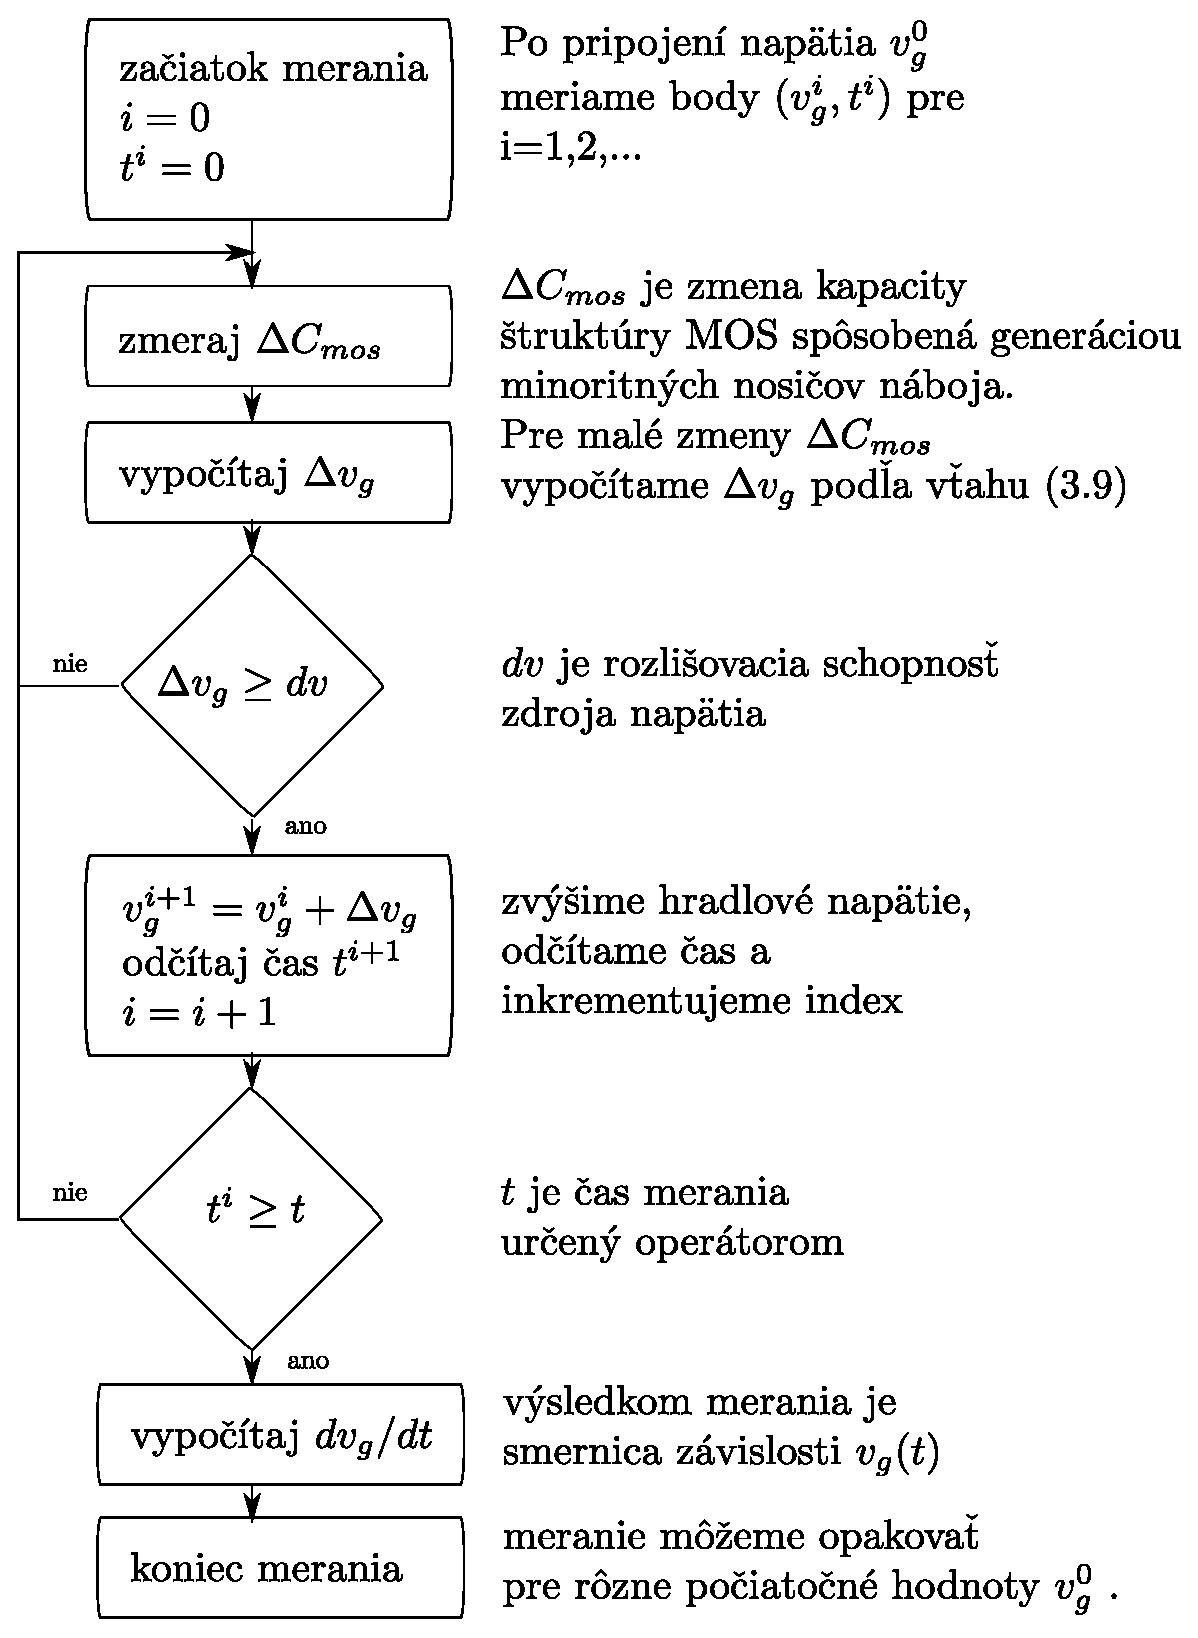
\includegraphics[width=\textwidth,height=\textheight,scale=0.7,keepaspectratio]{Figures/diagram-2.EPS}
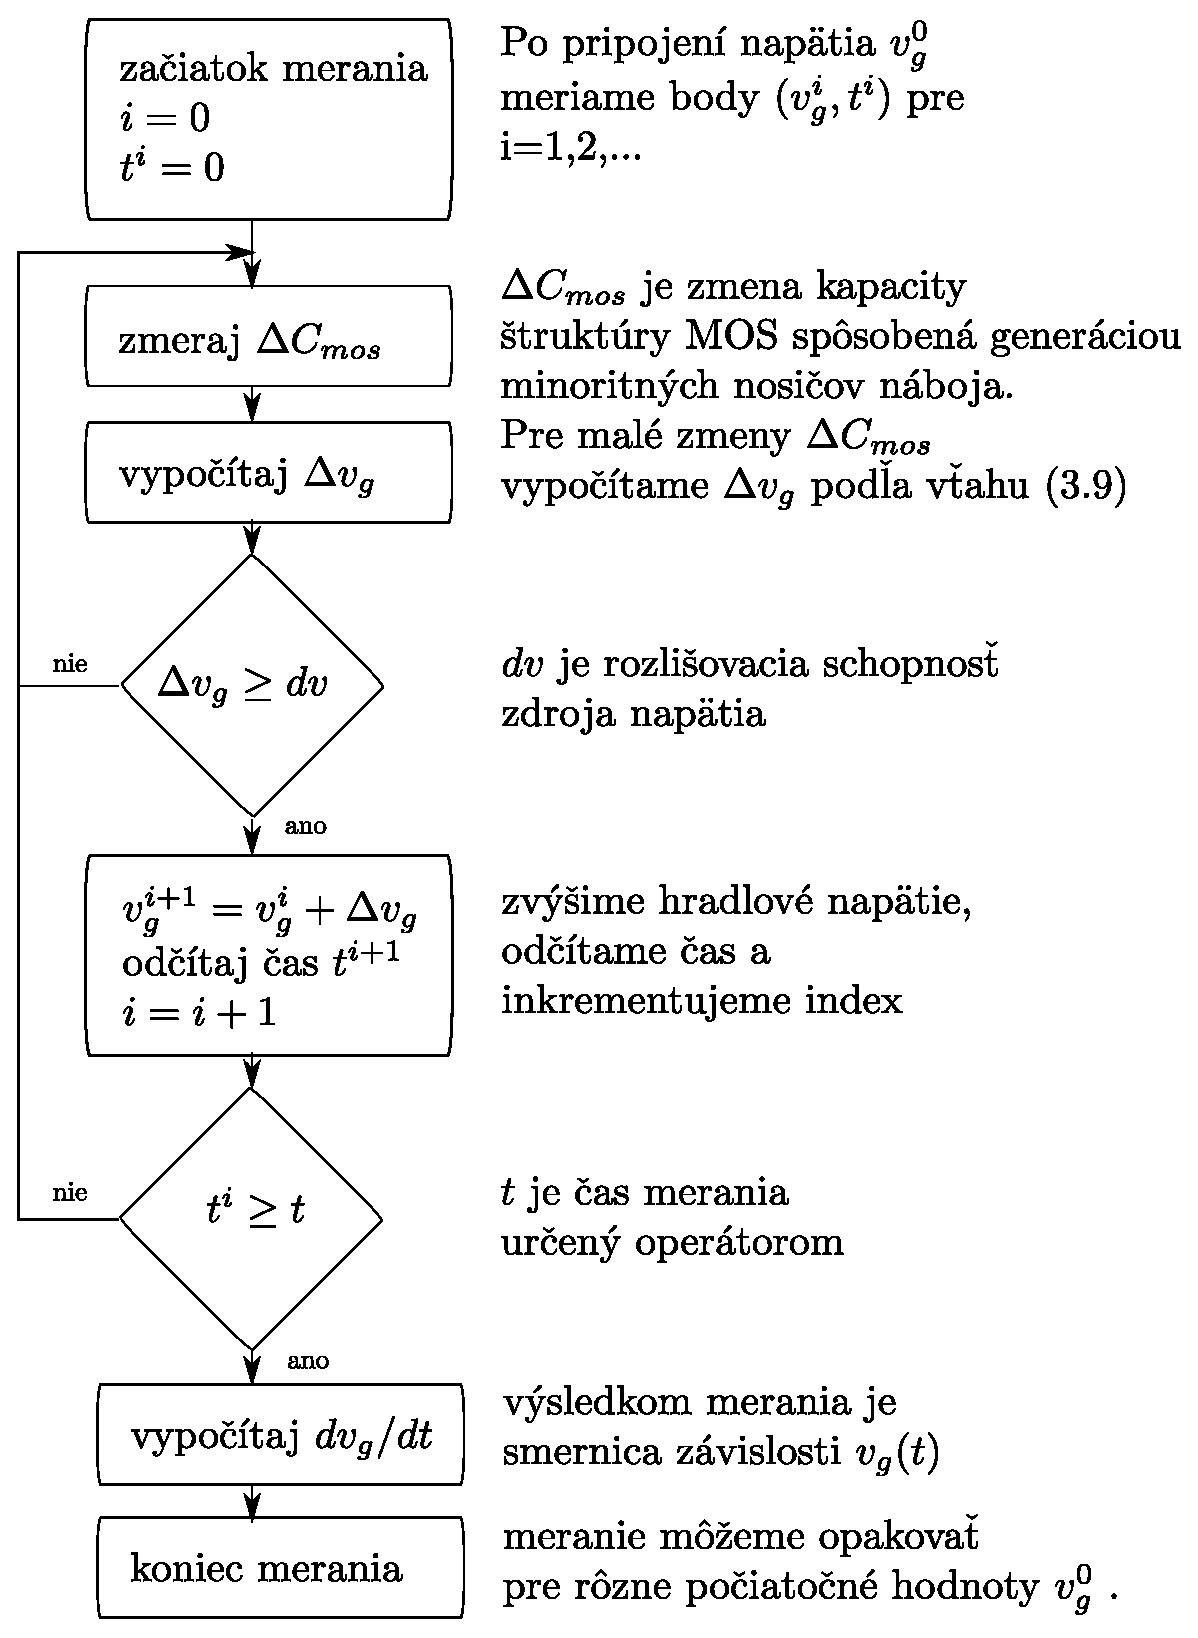
\includegraphics[scale=0.55,keepaspectratio]{Figures/diagram-2.EPS}
\label{diagram:2}
\end{diagram}

\begin{figure}[h!]\centering
%\framebox[10cm]{\rule{0cm}{3cm}}
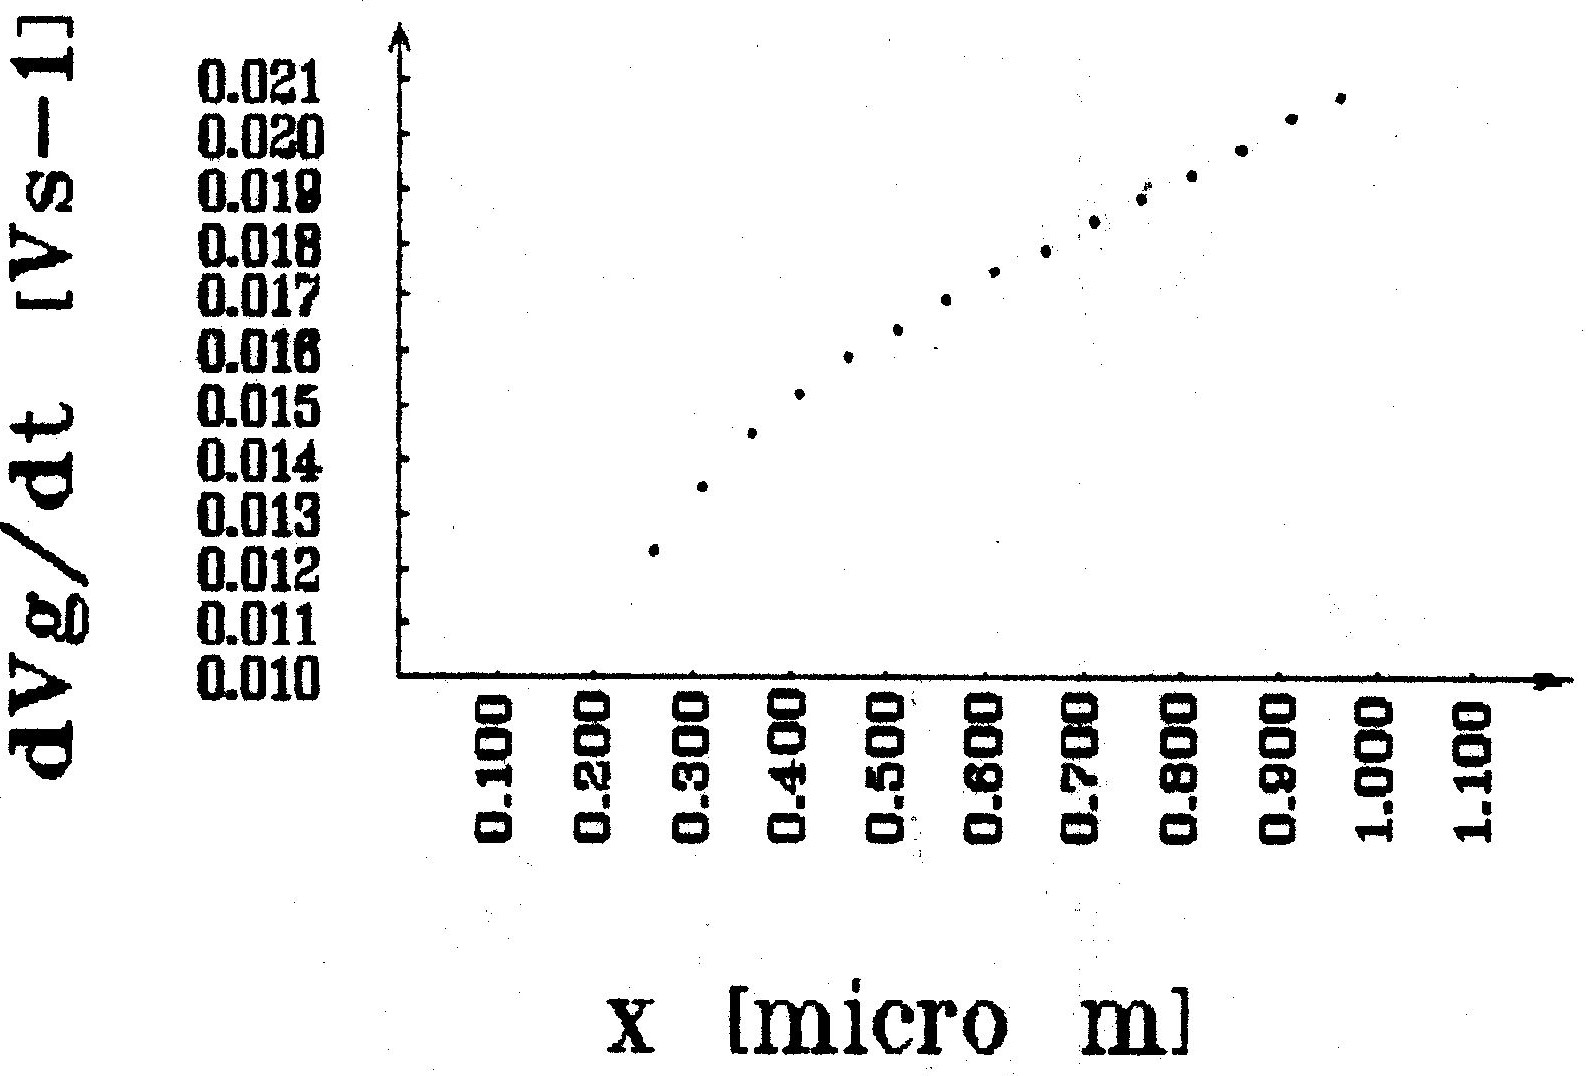
\includegraphics{Figures/fig-3-5.eps}
\captionsetup{justification=raggedright, singlelinecheck=false}
\caption[Závislosť $\frac{dV_g}{dt}$ od šírky OPN získaná pomocou
 metódy konštantnej šírky OPN]{Závislosť $\frac{dV_g}{dt}$ od šírky OPN
 získaná pomocou metódy konštantnej šírky OPN.}
\label{fig:3.5}
\end{figure}
%OBR19.BIT

Na obrázku \ref{fig:3.5} je znázornená závislosť $\frac{dV_g}{dt}$ od
šírky OPN.  Za predpokladu udržania konštantnej šírky OPN sa nemenia
potenciálové pomery v polovodiči a generácia minoritných nosičov je
konštantná, z čoho vyplýva linearita závislosti $V_g(t)$.  Smernice
$\frac{dV_g}{dt}$ potom možno určiť lineárnou regresiou nameraných
závislostí $V_g(t)$. Nie je ťažké si predstaviť, že vzťahy
\ref{eq:3.6} až \ref{eq:3.8} predstavujú diskretizáciu spojitého
priebehu $\tau_g(x)$. Ak namerané hodnoty $\frac{dV_g}{dt}=f(x)$
aproximujeme spojitou funkciou, môžeme vyjadriť hĺbkový profil
$\tau_g(x)$ vzťahom

\begin{equation}\label{eq:3.10}
\tau_g(x) = \frac{qn_i}{2C_{ox}} \Bigg[\frac{d\big[\frac{dV_g}{dt}\big]}{dx}\Bigg]^{-1}
\end{equation}

Na obrázku \ref{fig:3.6} je znázornený priebeh $\tau_g(x)$, vypočítaný
z nameraných dát zobrazených na obrázku \ref{fig:3.5} a na obrázku
\ref{fig:3.7} je hĺbkový koncentračný profil $N(x)$ skúmanej
štruktúry.

\begin{figure}[h!]\centering
%\framebox[10cm]{\rule{0cm}{3cm}}
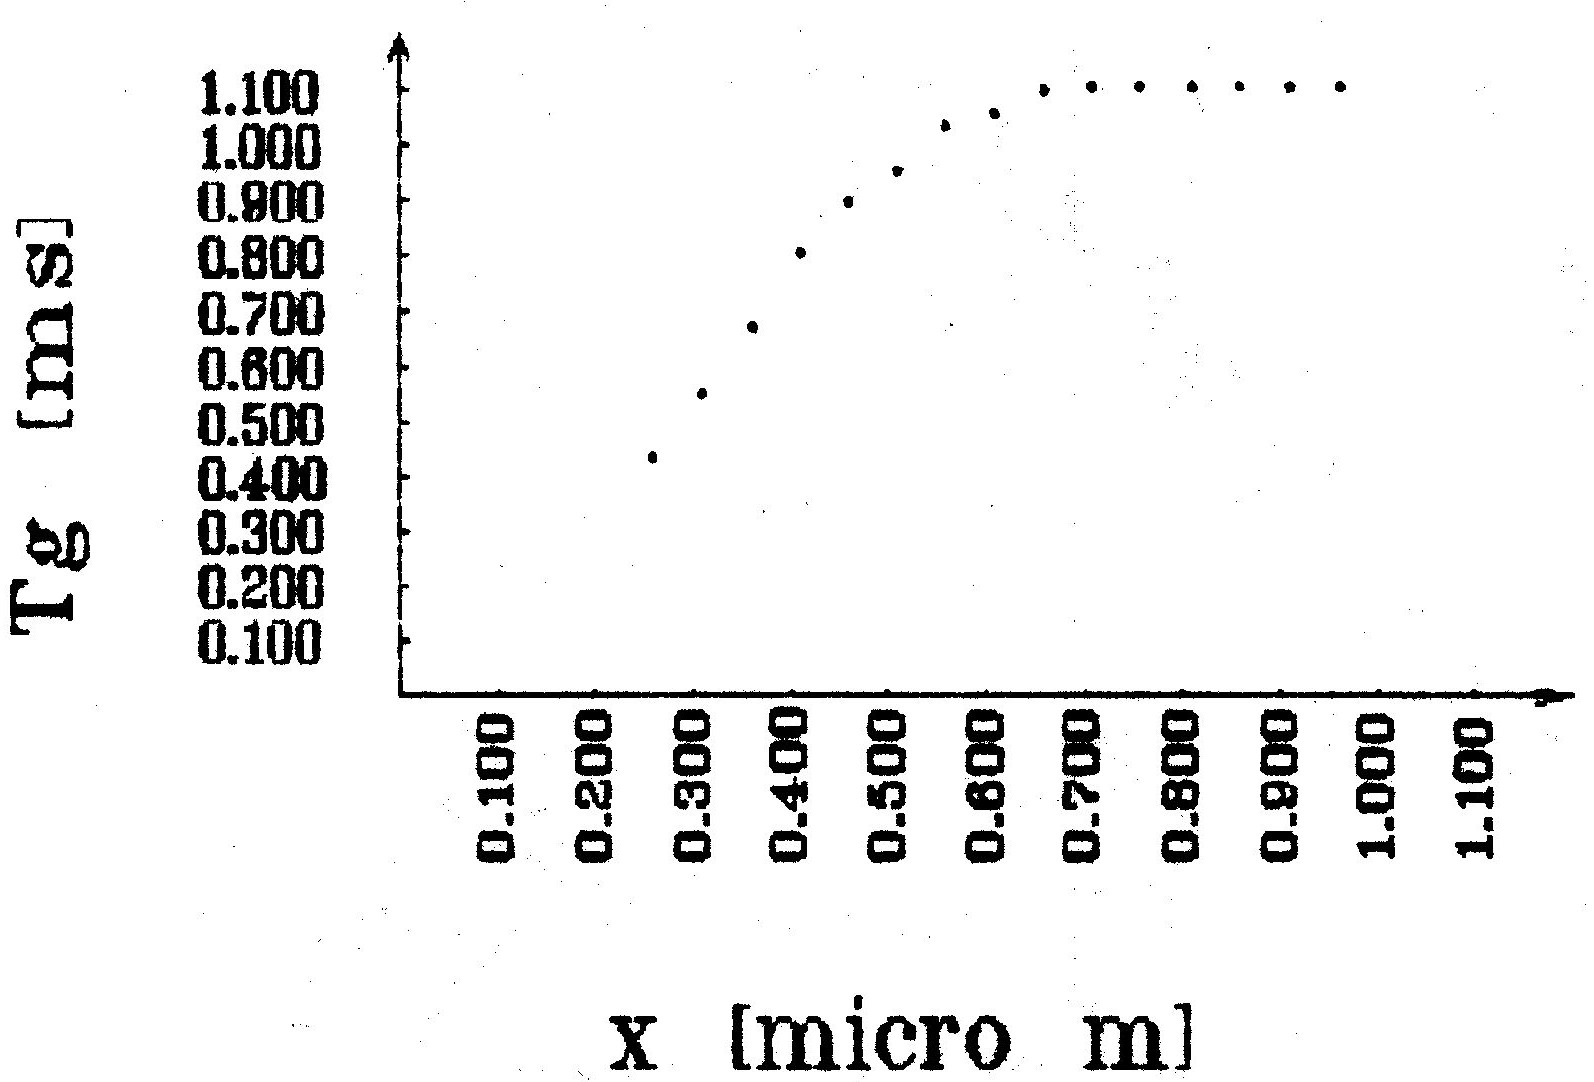
\includegraphics{Figures/fig-3-6.eps}
\captionsetup{justification=raggedright, singlelinecheck=false}
\caption[Hĺbkový profil generačného času života minoritných nosičov
  náboja]{Hĺbkový profil generačného času života minoritných nosičov
  náboja.}
\label{fig:3.6}
\end{figure}
%OBR20.BIT

\begin{figure}[h!]\centering
%\framebox[10cm]{\rule{0cm}{3cm}}
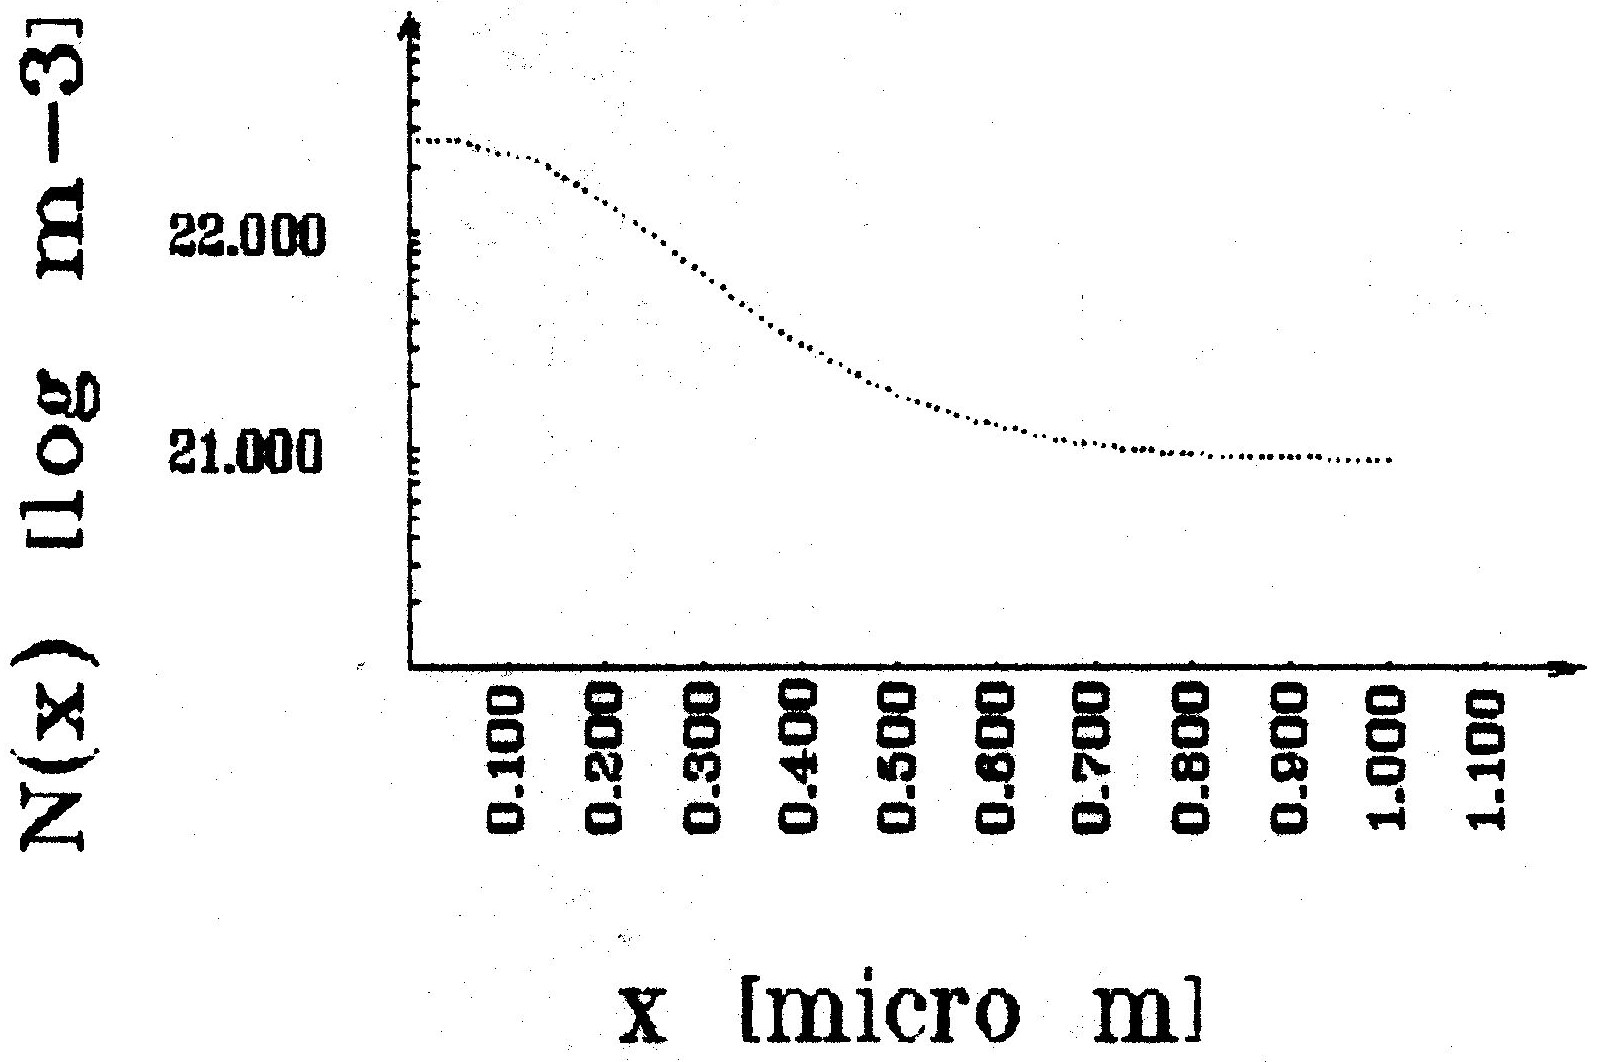
\includegraphics{Figures/fig-3-7.eps}
\captionsetup{justification=raggedright, singlelinecheck=false}
\caption[Hĺbkový profil koncentrácie dotujúcich prímesí
  $N(x)$]{Hĺbkový profil koncentrácie dotujúcich prímesí
  $N(x)$. Koncentračný profil prímesí bol vytvorený implantáciou
  $P^{31}$ s dávkou $8.0$ $10^{15}m^{-2}$ pri energii $120 keV$.
  Aktivácia prebiehala počas 40 minút pri teplote $1050 \degree C$ v
  atmosfére $N_2$.}
\label{fig:3.7}
\end{figure}
%OBR21.BIT


\begin{thebibliography}{}

\bibitem[3.1]{3.1}
Pierret R.F., Small D.W.: IEEE Trans. on elektron.dev. 22 (1975) s.1052.

\bibitem[3.2]{3.2}
Zerbst M.: Z. Angew. Phys. 22 (1966), s.30.

\bibitem[3.3]{3.3}
Eades W.D., Shott J.D., Swanson R.M.: IEEE Trans. on elektron. dev. 30 (1983) s.1274.

\bibitem[3.4]{3.4}
Nicollian E.H., Brews J.R.: Solid St. Electron.  27 (1984) s.953.

\bibitem[3.5]{3.5}
Ziegler K., Klausmann E.: Appl. Phys. Lett. 26 (1975) s.400.

\bibitem[3.6]{3.6}
Boulin D.M., Brews J.R., Nicollian E.H.: Solid St. Electron. 27  (1984) s.977.

\bibitem[3.7]{3.7}
Brews J.R., Nicollian E.H.: Solid  St. Electron. 27 (1984) s.963.

\bibitem[3.8]{3.8}
Botka V.,Csabay O., Jamrich M.: 5.celoštátna konferencia Mikroelektronika 1989, Dom techniky ČSVTS Bratislava, 1989 s.59.

\bibitem[3.9]{3.9}
Jamrich M.: Q-C metóda pre skúmanie štruktúr MIS. Diplomová práca, Katedra mikroelektroniky, EF SVŠT, Bratislava 1988.

\bibitem[3.10]{3.10}
Beyer A., Markgraf W.: Wiss. Z. d. Techn. Hochsch. Karl-Marx-Stadt 28 (1986) s.479.

\bibitem[3.11]{3.11}
Lal, Vasi: Solid St. Electron. 30 (1987) s.801.

\bibitem[3.12]{3.12}
Hof, Morthers, Roenker: Solid St. Electron. 31 (1988) s.937.

\bibitem[3.13]{3.13}
Pilka K.: Nerovnovážna kapacitná metóda s konštantnou šírkou OPN, Katedra mikroelektroniky, EF SVŠT, Bratislava 1989.

\end{thebibliography}

% Chapter 4

\chapter{Methods for determining other parameters of the MOS structure.}\label{Chapter4}
\lhead{Chapter 4. \emph{Methods of determining other parameters of the MOS structure}}
%- - - - - - - - - - - - - - - - - - - - - - - - - - - - - - - - - - - - - - - - - - - -

In Chapter~\ref{Chapter3} we have described the C-V methods that we
will use to determine the parameters of MOS\@ structures. In
particular, we we will deal with the determination of the
concentration profile of the donating impurities in the subsurface
region of the semiconductor, since some methods of determining other
MOS structure parameters are based on the assumption that the
concentration is known. In determining the concentration profile
waveforms, which are not homogeneous, models are used whose accuracy
of approximating a given physical phenomenon depends on the
concentration gradient admixture~\cite{4.1, 4.2, 4.3, 4.4}. In order
to verify the accuracy of the used approximations, we performed a
comparison of the concentration profiles:

\begin{itemize}
\item used in the calculation of the theoretical C-V dependence and
\item obtained from this theoretical C-V dependence~\cite{4.5}.
\end{itemize}

The results are given in Section~\ref{sec:4.1.4}.

\par The next parameter we will determine is the density of traps
of the $Si-SiO_{2}$ interface. Here, two
procedures. Comparison of high and low frequency C-V
dependence, or a comparison of experimental and theoretical C-V
dependence. Their application is described in Section~\ref{sec:4.2}.

\par Determination of the generation lifetime of minority charge carriers that
related to the constant-width OPN method, has been described in Section~\ref{sec:3.4}.

\section[Determination of the concentration profile of impurities]{Determination of the concentration profile of impurities in the subsurface region of the semiconductor.}\label{sec:4.1}

The issue of measuring concentration profiles was in our department in
our department in paper~\cite{4.6}. Here we will deal only with some
aspects of this issue that are related to the determination of
inhomogeneous concentration profile of impurities in a semiconductor.

\par Separate areas of concern in determining the concentration
profile of impurities, which we denote by $N(x)$, consist of:

\begin{itemize}
\item correction of the calculated concentration in the region from
  the surface of the semiconductor to a depth of $2L_{DE}$~\cite{4.7,
    4.8}
\item determination of the depth of the calculated concentration,
  relying on models determining the width of the OPN~\cite{4.9, 4.10,
    4.11}
\item correction for the effect of $Si-SiO_2$ interface
  traps~\cite{4.12}
\item the difference between the concentration of the interfering
  impurities $N(x)$ and the concentration of the majority charge
  carriers $n(x)$.
\end{itemize}

We will deal with the above problems in turn.

\subsection[Correction of the concentration of interfering impurities]{Correction of the concentration of interfering impurities at the surface of the semiconductor.}\label{sec:4.1.1}

Known relationship for calculating $N(x)$~\cite{I.2}

\begin{equation}\label{eq:4.1}
  N(x) = {\frac{2}{q\epsilon}} {\Bigg[\frac{dC_{sc}^{-2}}{d\varphi_{s}}\Bigg]}^{-1}
\end{equation}

was derived from the solution of the Poisson equation using the
approximation of deep impoverishment. This approximation does not hold
for OPN widths smaller than $2L_{DE}$.  In order to obtain correct
results in this region as well, we need to correct $N(x)$ computed
according to~\ref{eq:4.1} by the procedure derived in~\cite{4.7, 4.8}.
From the work of~\cite{4.7} it is also evident the physical
significance of this correction, which is a function of the surface
potential

\begin{equation}\label{eq:4.2}
  {N(x)}_{corrected} = N(x)f(\varphi_{s})
\end{equation}

, where

\begin{equation}\label{eq:4.3}
  f(\varphi_{s}) = {\frac{1}{1-e^{-\beta\varphi_{s}}}} - {\frac{2e^{-\beta\varphi_{s}}\big[e^{-\beta\varphi_{s}}+\beta\varphi_{s} -1\big]}{\big[1-e^{-\beta\varphi_{s}}\big]}} \qquad, where\quad \beta=\frac{q}{kT}
\end{equation}

The surface potential used in relation~\ref{eq:4.3} can be determined
according to~\cite{4.7} by numerically solving the equation

\begin{equation}\label{eq:4.4}
  \frac{C_{sc}^{2}}{\varphi_{s}}\frac{C_{sc}^{-2}}{d\varphi_{s}}=\frac{1-e^{-\beta\varphi_{s}}}{e^{-\beta\varphi_{s}}+\beta\varphi_{s}-1}-\frac{2e^{-\beta\varphi_{s}}} {1-e^{-\beta\varphi_{s}}}
\end{equation}

It should be noted here that the relation~\ref{eq:4.4} was derived
using the relation for the OPN capacity $C_{sc}$, which assumes a
homogeneous concentration impurities. Since the experimentally
determined differential capacitance $C_{sc}$ depends on the change in
charge at the OPN boundary (which uses relation~\ref{eq:4.1}), the
surface potential obtained from relation~\ref{eq:4.4} will represent
the potential that would be at the surface the semiconductor if the
concentration of $N(x)$ across the OPN region were constant and also
equal to the concentration at the OPN boundary (which we determine
according to~\ref{eq:4.1}). It follows that for inhomogeneously
endowed substrates using the relation~\ref{eq:4.4} cannot be used to
obtain the true $\varphi_{s}(V_{g})$, despite the fact that the
correction~\ref{eq:4.2} gives good results in this case as well.

\subsection[Determination of the depth of the concentration profile.]{Determination of the depth of the concentration profile.}\label{sec:4.1.2}

Having determined the concentration according to the
relation~\ref{eq:4.2}, it is also necessary to determine the location
of the calculated concentration. A commonly used relationship based on
plate capacitor model (which is an approximation of the deep
depletion)

\begin{equation}\label{eq:4.5}
  w(C_{sc})=\frac{\epsilon}{C_{sc}}
\end{equation}

is not valid for depths less than $2L_{DE}$. In this region, the a
relation derived using an approximation of the potential waveform in a
semiconductor $\varphi(x)$. The above problem has been discussed in
detail in our department treated in detail in~\cite{4.13, 4.14}, when
the results of work~\cite{4.9, 4.10, 4.11} were used. To calculate the
depth in this region we can use a relation that is an approximation of
the potential waveform in semiconductor $\varphi(x)$~\cite{I.1}

\begin{equation}\label{eq:4.6}
  w(\varphi_{s})=\sqrt{2}L_{DE}{\big[e^{-\beta\varphi_{s}}+\beta\varphi_{s}-1\big]}^{\frac{1}{2}}
\end{equation}

, where

\begin{equation}\label{eq:4.7}
  L_{DE} = {\Big[\frac{\epsilon}{\beta qN}\Big]}^{\frac{1}{2}}
\end{equation}

is the extrinsic Debay length, which we used in the calculation the
concentration obtained from the relation~\ref{eq:4.2}.  In
relation~\ref{eq:4.6} we use the value of $\varphi_{s}$ obtained from
the solution relation~\ref{eq:4.4}. Despite the fact that also the
relation~\ref{eq:4.6} was derived assuming a homogeneous distribution
of impurities in the semiconductor, its use in conjunction with the
solution of equation~\ref{eq:4.4} gives a satisfactory results, as we
shall show later.

\begin{figure}[h!]\centering
  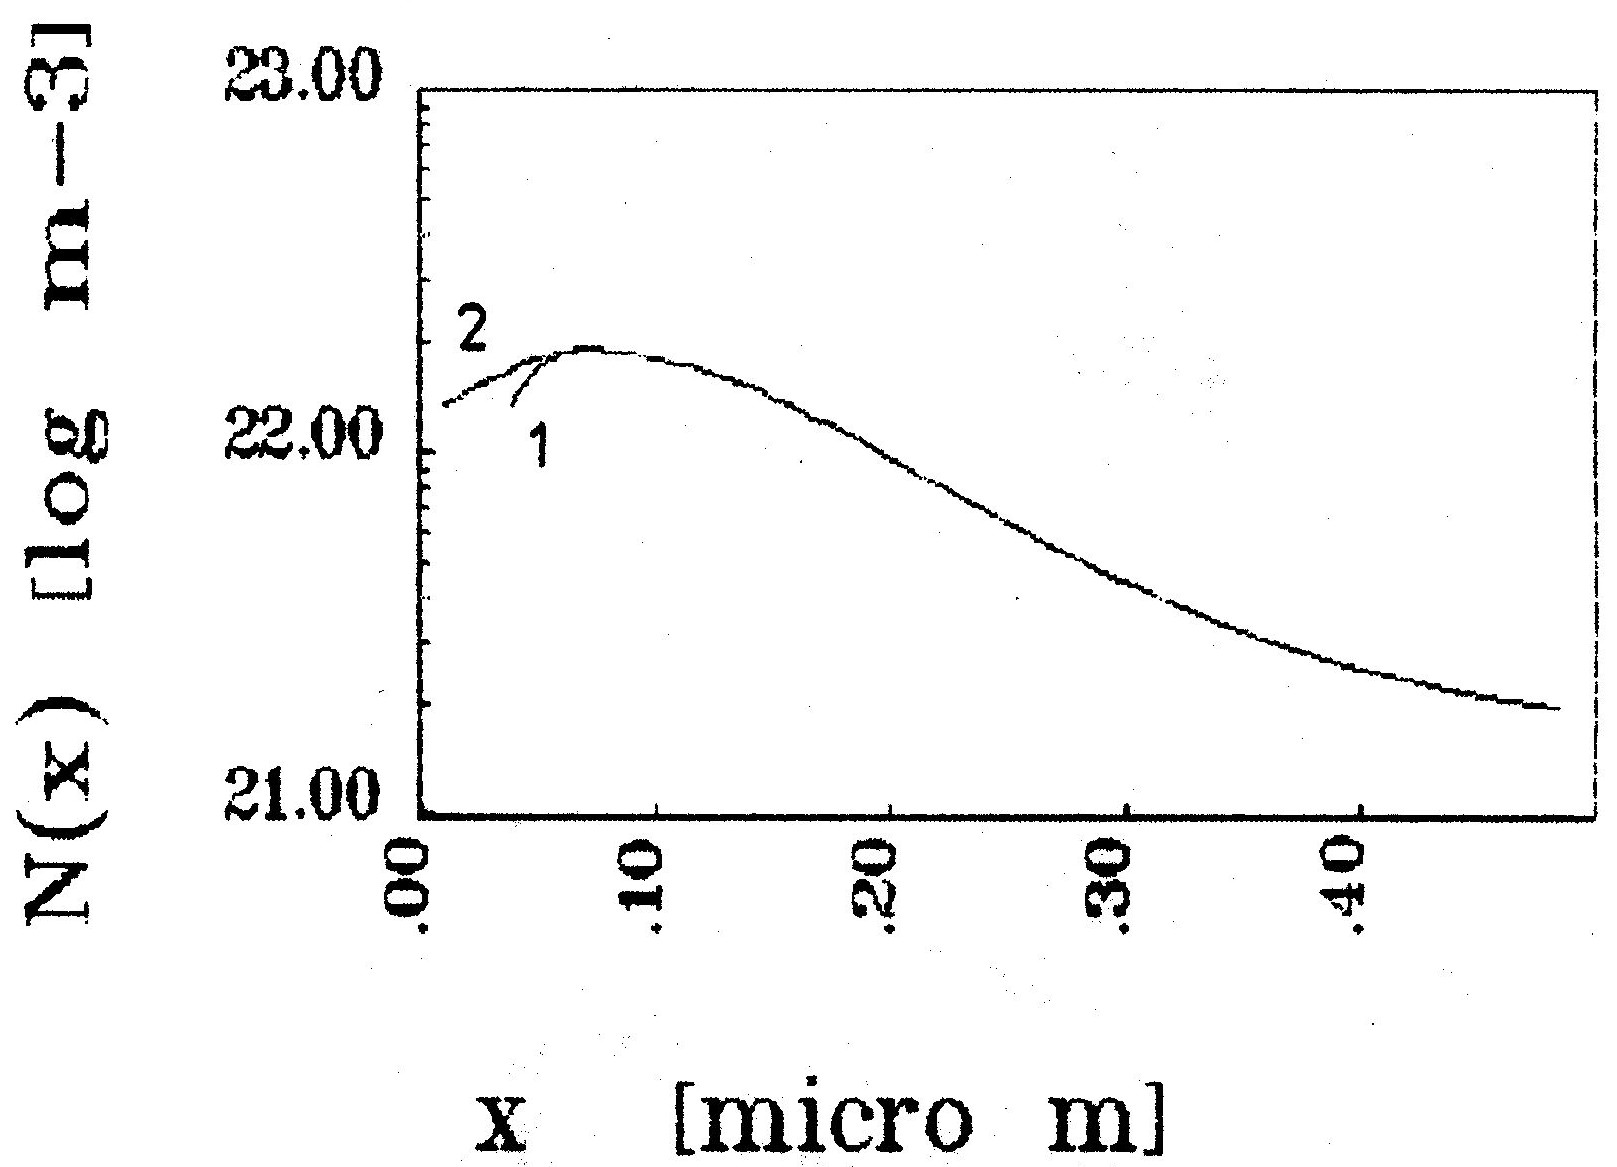
\includegraphics{Figures/fig-4-1.eps}% chktex-file 8
  \caption[Concentration profile of dopants in a semiconductor
    calculated from the relation~\ref{eq:4.2}]{Concentration profile
    of the dopants in the semiconductor calculated from the
    equation~\ref{eq:4.2}. The distance from the surface was
    determined from the equation~\ref{eq:4.5} (curve 1)
    and~\ref{eq:4.6} (curve 2).}\label{fig:4.1}
\end{figure}
% OBR26.BIT

Figure~\ref{fig:4.1} shows the waveforms of $N(x)$ using
correction~\ref{eq:4.2}, presenting the difference in using
relations~\ref{eq:4.5} and~\ref{eq:4.6}. Here it is clear that by
using relation~\ref{eq:4.6}, one can calculate the path of the
concentration of the interfering of impurities closer to the
semiconductor surface, which is of importance for further
calculations, which presuppose knowledge of the $N(x)$ waveform.

The first column of the spreadsheet~{tab:4.1} contains the values of
$\varphi_{s}$ determined by by solving equation~\ref{eq:4.4} and the
second column contains the values of of the correction
factor~\ref{eq:4.3}. The other two columns allow comparison the
uncorrected and corrected values of $N(x)$ and in the last two columns
give the values of $w(\varphi_{s})$ and $w(C_{sc})$ obtained from
relations~\ref{eq:4.5} and~\ref{eq:4.6}.

\begin{table}[h!]\centering
  \begin{tabular}{c c c c c c c c c c}
    $\varphi_{s}[V]$ & $f(\varphi_{s})$ & $N[m^{-3}]$ & $N_{cor.}[m^{-3}]$ & $w(\varphi_{s})[\mu m]$ & $w(C_{SC})[\mu m]$ \\
    \hline% chktex-file 44
    0.007 & 0.39 & $0.35\times10^{23}$ & $0.14\times10^{23}$ & 0.0102 & 0.0389 \\
    0.016 & 0.44 & $0.33\times10^{23}$ & $0.15\times10^{23}$ & 0.0190 & 0.0413 \\
    0.024 & 0.50 & $0.31\times10^{23}$ & $0.15\times10^{23}$ & 0.0265 & 0.0438 \\
    0.032 & 0.56 & $0.29\times10^{23}$ & $0.16\times10^{23}$ & 0.0333 & 0.0466 \\
    0.041 & 0.61 & $0.28\times10^{23}$ & $0.17\times10^{23}$ & 0.0391 & 0.0494 \\
    0.049 & 0.66 & $0.27\times10^{23}$ & $0.18\times10^{23}$ & 0.0444 & 0.0523 \\
    0.057 & 0.71 & $0.26\times10^{23}$ & $0.18\times10^{23}$ & 0.0493 & 0.0553 \\
    0.065 & 0.76 & $0.25\times10^{23}$ & $0.19\times10^{23}$ & 0.0538 & 0.0585 \\
    0.073 & 0.80 & $0.24\times10^{23}$ & $0.19\times10^{23}$ & 0.0581 & 0.0617 \\
    0.081 & 0.83 & $0.23\times10^{23}$ & $0.19\times10^{23}$ & 0.0623 & 0.0650 \\
    0.090 & 0.86 & $0.22\times10^{23}$ & $0.19\times10^{23}$ & 0.0664 & 0.0684 \\
    0.098 & 0.89 & $0.22\times10^{23}$ & $0.19\times10^{23}$ & 0.0704 & 0.0719 \\
    0.106 & 0.91 & $0.21\times10^{23}$ & $0.19\times10^{23}$ & 0.0743 & 0.0755 \\
    0.115 & 0.93 & $0.21\times10^{23}$ & $0.19\times10^{23}$ & 0.0783 & 0.0791 \\
    0.124 & 0.94 & $0.20\times10^{23}$ & $0.19\times10^{23}$ & 0.0822 & 0.0828 \\
    0.133 & 0.96 & $0.20\times10^{23}$ & $0.19\times10^{23}$ & 0.0861 & 0.0866 \\
    0.142 & 0.97 & $0.19\times10^{23}$ & $0.19\times10^{23}$ & 0.0900 & 0.0904 \\
    0.151 & 0.97 & $0.19\times10^{23}$ & $0.18\times10^{23}$ & 0.0939 & 0.0942 \\
    0.160 & 0.98 & $0.19\times10^{23}$ & $0.18\times10^{23}$ & 0.0978 & 0.0981 \\
    0.169 & 0.99 & $0.18\times10^{23}$ & $0.18\times10^{23}$ & 0.1018 & 0.1019 \\
    0.178 & 0.99 & $0.18\times10^{23}$ & $0.18\times10^{23}$ & 0.1058 & 0.1058 \\
    0.187 & 0.99 & $0.18\times10^{23}$ & $0.17\times10^{23}$ & 0.1098 & 0.1098 \\
    0.205 & 1.00 & $0.17\times10^{23}$ & $0.17\times10^{23}$ & 0.1179 & 0.1179 \\
  \end{tabular}
  \caption[Calculation of dopant concentration profile
    $N(x)$]{Calculation of dopant concentration profile
    $N(x)$.}\label{tab:4.1}
\end{table}


\emph{NOTE.}

Using the approximation~\ref{eq:4.6}, which represents the width of
the OPN as as a function of the surface potential of the semiconductor
(the concentration is parameter), one can approximate the path of
$\varphi(x)$ for a given OPN width even if the semiconductor substrate
is inhomogeneously doped.  Custom procedure for determining the
concentration of dopant impurities from capacitance measurements is a
discretization of the continuous $N(x)$ waveform, where the individual
values of $N_i$ represent an approximation of the concentration in the
region of the boundary OPN~\cite{4.1, 4.2, 4.3}.  The loss of the
potential $\Delta\varphi_i$ at layer of width $\Delta
w_{i}=w_{i+1}-w_{i}$ with concentration $N_i$ can be determined by
solving the equation

\begin{equation}\label{eq:4.8}
  \Delta w_{i} = \sqrt{2}L_{DE_{i}}{\Big[e^{-\beta\Delta\varphi_{i}} + \beta\Delta\varphi_{i} - 1\Big]}^{\frac{1}{2}}
\end{equation}

, where

\begin{equation}\label{eq:4.9}
  L_{DE_{i}} = {\bigg[\frac{\epsilon}{\beta qN_{i}}\bigg]}^{\frac{1}{2}}
\end{equation}

Then the progression of $\varphi(x)$ can be obtained using the
equations~\ref{eq:4.8} and~\ref{eq:4.9} if we start the calculation
from the OPN boundary, where we assume potential is zero, towards the
surface of the semiconductor.


\subsection[Effect of $Si-SiO_{2}$ interface traps and minority charge carrier generation]{Effect of $Si-SiO_{2}$ interface traps and minority charge carrier generation}\label{sec:4.1.3}

Minority carrier generation occurs in the inversion region of the OPN
charge generation, which forms the inversion layer and affects the
magnitude of the capacitance of the MOS\@ structure. In order to
measure the C-V dependence in the deep depletion that is not affected
by minority charge carriers, we will use the pulsed HF C-V method. The
measured values of $N(x)$ obtained using this method are shown in
Figure~\ref{fig:4.2}.

\begin{figure}[h!]\centering
  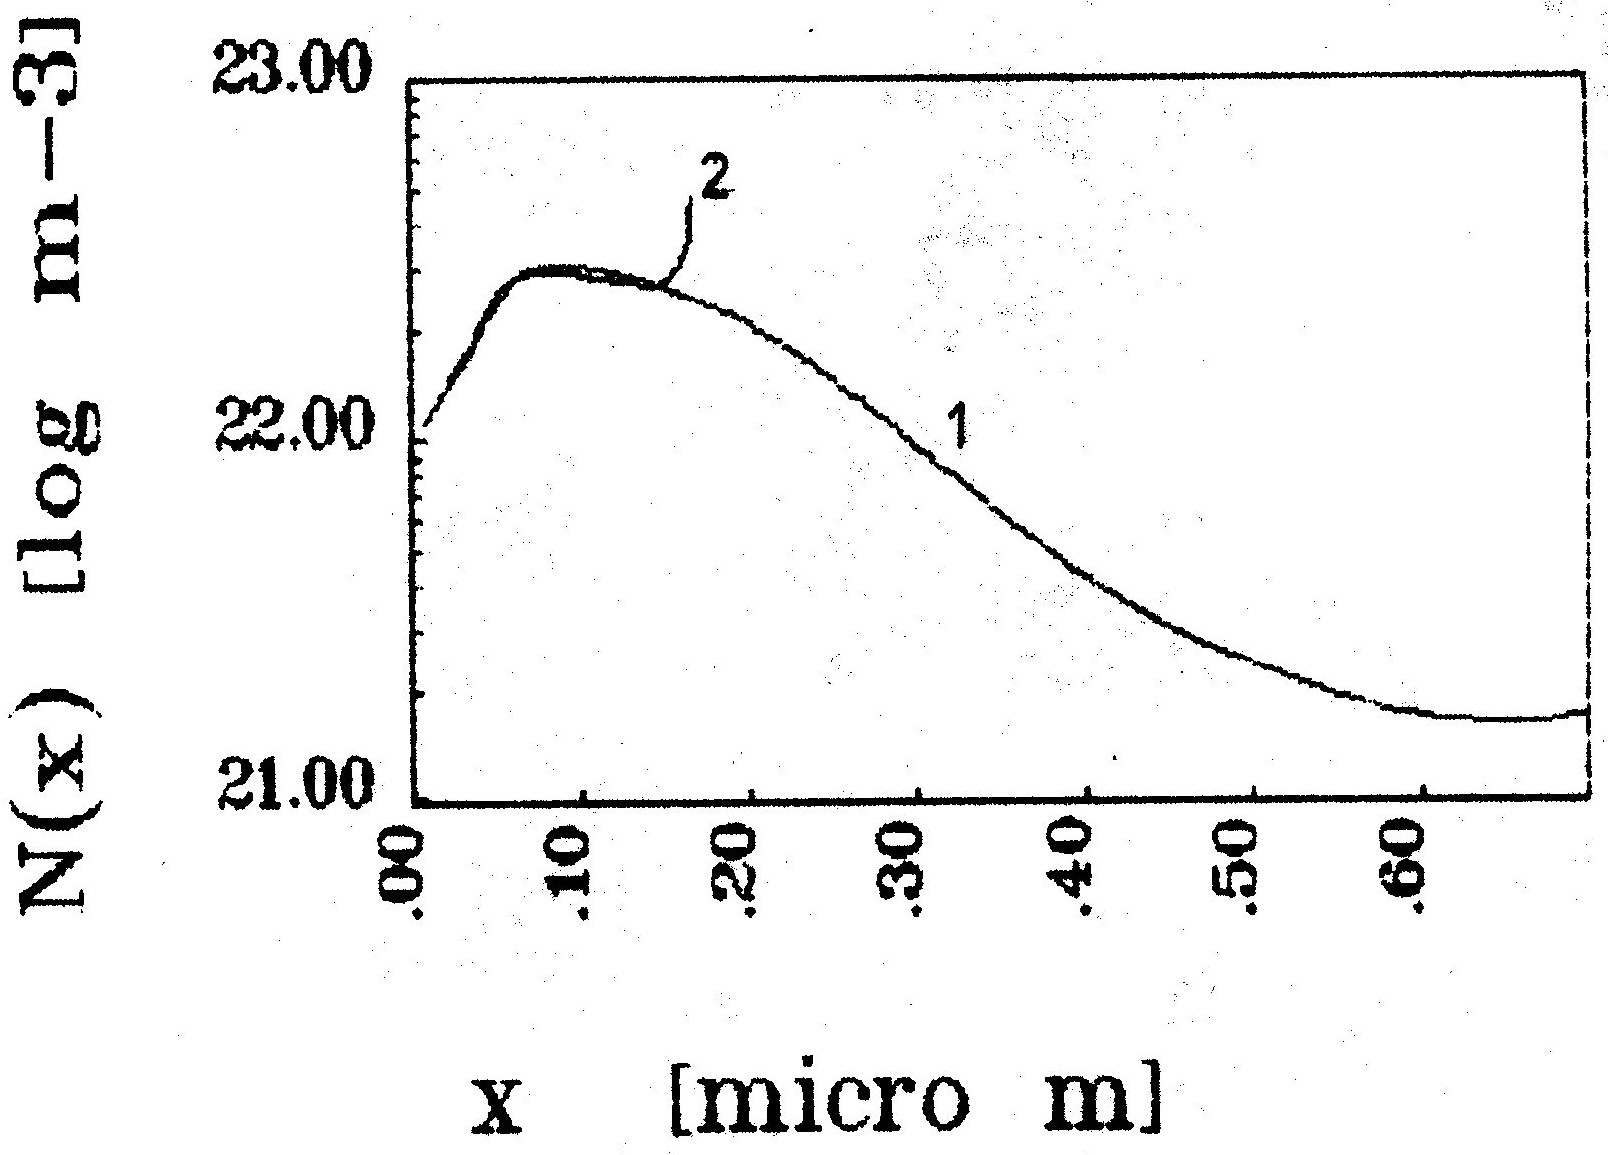
\includegraphics{Figures/fig-4-2.eps}% chktex-file 8
  \caption[Concentration profile of interfering impurities obtained
    from C-V dependence in the deep depletion region and from the
    equilibrium C-V dependence]{Current concentration profile of the
    interfering impurities obtained from the C-V dependence in the
    deep depletion region (curve 1) and from the equilibrium C-V
    dependence (curve 2). To calculate $N(x)$ dependence, the C-V
    dependences shown in Figure~\ref{fig:3.2}}\label{fig:4.2}
\end{figure}
% OBR8.BIT

\par When calculating $N(x)$ using
equations~\ref{eq:4.1},~\ref{eq:4.2},~\ref{eq:4.3},~\ref{eq:4.4}
and~\ref{eq:4.6} the approximation is used

\begin{equation}\label{eq:4.10}
  \frac{dC_{sc}^{-2}}{d\varphi_{s}} \cong \frac{dC_{mos}^{-2}}{dV_{g}}
\end{equation}

where equality holds if the trap density of the $Si-SiO_{2}$ interface
is zero. However, the measured HF C-V dependence is always to some
extent affected by the interface traps, which change their
state~\cite{4.15}. This influence can be reduced by increasing the
frequency of the measurement signal and by measuring the capacitance
faster after the voltage jump pulsed C-V method.  The problem of using
the approximation~\ref{eq:4.10} is avoided if we use the data measured
by Q-C to determine $N(x)$ method, where we can determine the surface
potential waveform $\varphi_{s}(V_{g})$.

\par If we determine the concentration profile of the dopants from the
HF C-V dependence, we can correct for the effect of the $Si-SiO_{2}$
interface traps in depletion region by the relation given
in~\cite{I.1}

\begin{equation}\label{eq:4.11}
  {N(x)}_{corrected} = {N(x)}{\frac{1-\frac{C_{mos}^{LF}}{C_{ox}}}{1-\frac{C_{mos}^{HF}}{C_{ox}}}}
\end{equation}

assuming we know the low-frequency C-V dependence.

\subsection[Calculation of the concentration profile of the interfering impurities from the major charge carrier waveform and validation of the models used.]{Calculation of the concentration profile of the interfering impurities from the major charge carrier waveform and validation of the models used.}\label{sec:4.1.4}

As can be seen from Figure~\ref{fig:1.1}, for the inhomogeneous
waveform of the concentration of the donor atoms occurs due to
diffusion of the majority charge carriers, there is a difference
between the above waveforms~\cite{4.16}. It known~\cite{4.17} that by
using the relation~\ref{eq:4.1} we determine the waveform of the
concentration of the majority charge carriers instead of the
concentration of the contaminating impurities. A correction is
described in the work of~\cite{4.18}, using the which can be used to
determine the exact concentration of the interfering atoms from the
measured $n (x)$ (if the measured $n (x)$ actually represents the
waveform of the major charge carriers).

\begin{figure}[h!]\centering
  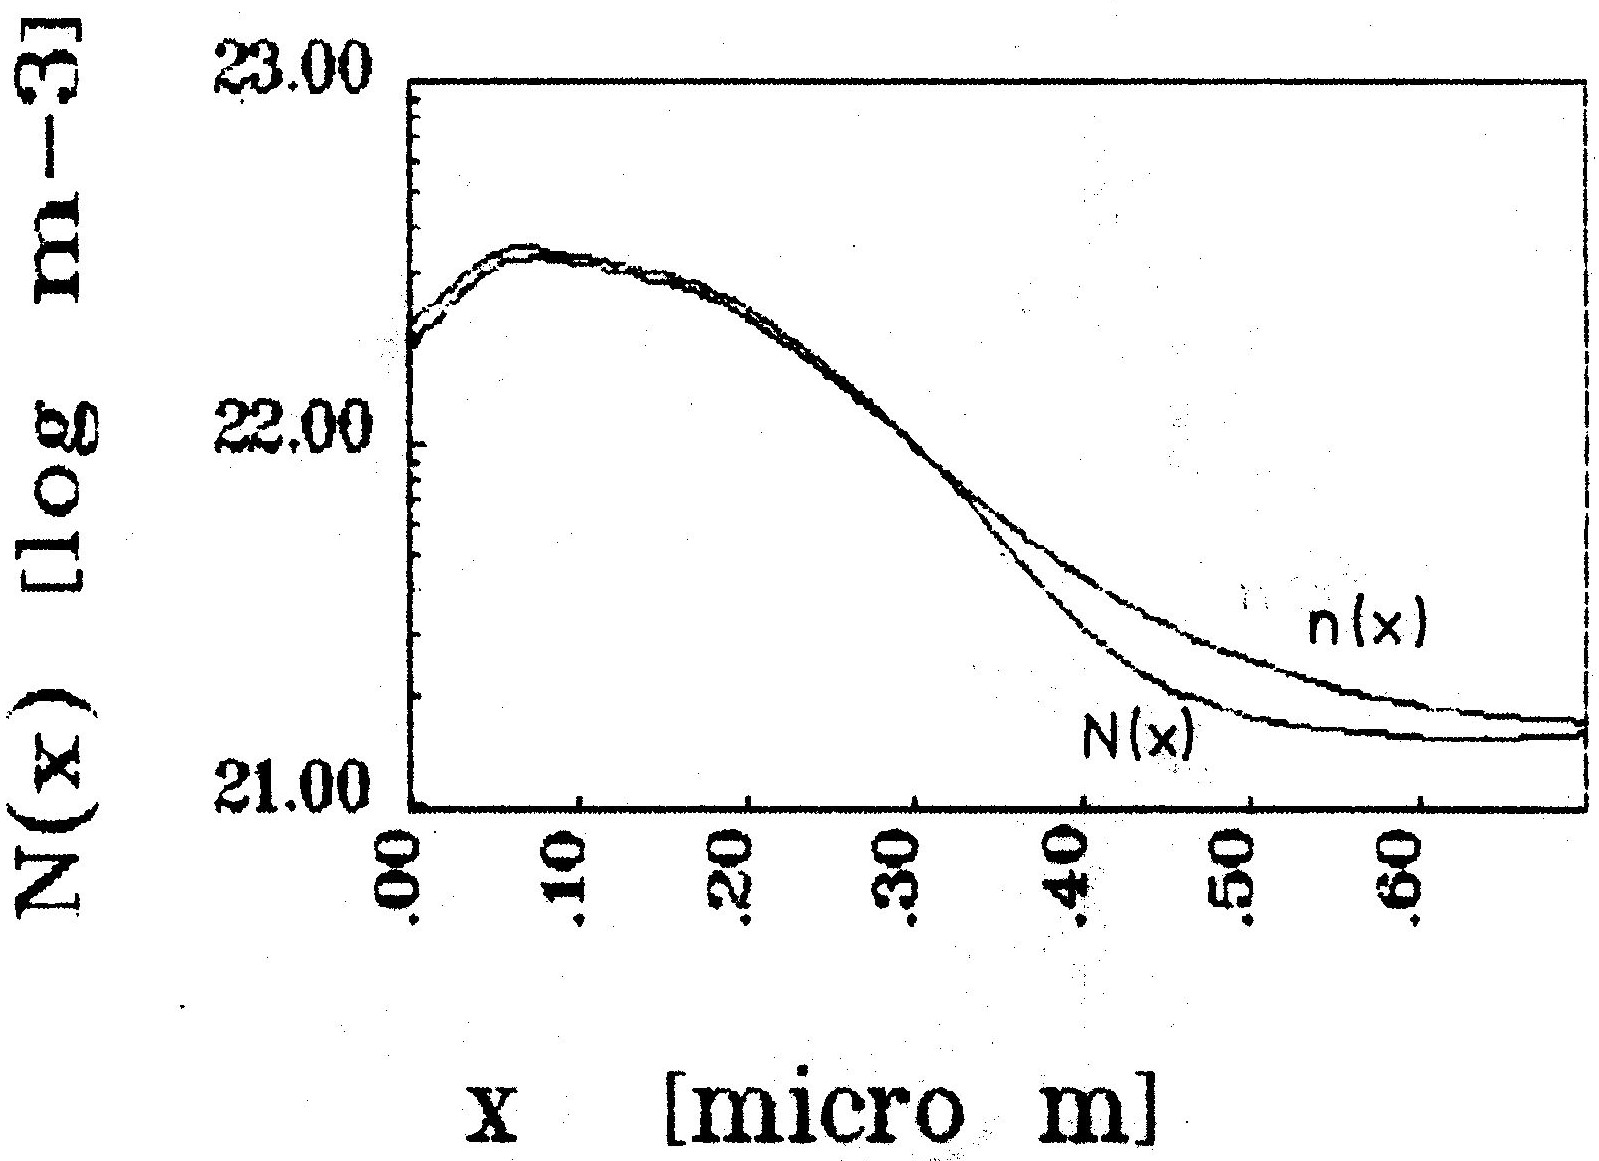
\includegraphics{Figures/fig-4-3.eps}
  \caption[Majority charge carrier concentration $n(x)$ determined
    from the depleted HF C-V dependence and the progression of the
    donating atoms $N (x)$ determined from the
    equation~\ref{eq:4.12}]{Concentration waveform of major charge
    carriers $n (x)$ determined from the depleted HF C-V dependence and
    the path of the $N (x)$ donor atoms determined from
    equation~\ref{eq:4.12}.}\label{fig:4.3}
\end{figure}
% OBR23.BIT

\begin{equation}\label{eq:4.12}
  N(x) = n(x) - {\frac{kT\epsilon}{q^{2}} {\frac{d}{dx}} {\Bigg[\frac{1}{n(x)}\frac{dn(x)}{dx}\Bigg]}}
\end{equation}

Figure~\ref{fig:4.3} shows the waveforms of $n(x)$ and $N(x)$. In
relation~\ref{eq:4.12} the second derivative of $n(x)$ stands out,
which in the case of experimental values of $n(x)$ must be determined
numerically.

\par Determining the derivative of an empirically obtained functional
dependence is a problem that can often be encountered when processing
measured data. In the basic numerical mathematics courses~\cite{4.19}
it is shown that differentiation amplifies the noise of the processed
data. In doing so, noise here generally refers to the deviation of the
processed data from its actual value that may arise as a consequence
of:

\begin{itemize}
\item physical phenomena
\item measurement instrument error
\item rounding in numerical processing.
\end{itemize}

\par That is, the frequency spectrum of the processed signal, obtained
by Fourier transformation, will contain components that must be
removed before (or during) the derivative calculation. V the
following we will talk about the approximation by polynomials, which
most commonly used, although the above statements also apply to other
classes of functions.

\par If we use polynomial approximations to calculate the derivative,
the it is convenient to `smooth'~\cite{4.20} the function values
first. To suppress noise suppression, the frequency properties of the
numerical methods, which can be expressed in terms of the transfer
characteristics. This approach we can compare the frequency properties
of polynomial approximations and numerical filters~\cite{4.21}.  The
basic difference between the calculation of the coefficients of
digital filters and the coefficients of of polynomial approximations
is that in the first case we start from the desired transmission
characteristic and in the latter case are coefficients are calculated
from the least squares distance condition of the processed data and
the polynomial of a given degree. Hence shortcomings of polynomial
approximations:

\begin{itemize}
\item processed functional dependence may not be a polynomial, even
  though there is a polynomial that interpolates the measured values
\item frequency properties of the method are a secondary consequence
  of the degree of the polynomial used and the number of points
  through which the polynomial translates.
\end{itemize}

\par Because in our case we are processing functional dependencies
that are not polynomials in general, we have chosen to use numerical
filters. It may be mentioned here that for a successful application of
digital filters is important to design the critical frequency and
magnitude of the filter so that the filter does not affect the
amplitude of the signal in that part of the of the spectrum that
represents the useful signal. To determine the derivatives in
formula~\ref{eq:4.12}, we used a non-recursive differentiating
low-pass digital filter whose critical frequency is $f_{c}=0.1$ and
its size is $2n+1=11$.

\par It is known~\cite{4.18} that even the progression of $n(x)$,
determined from the measured C-V dependence, is subject to error if it
represents a non-homogeneous concentration profile. More precisely, it
can be argued~\cite{4.3} that the measured concentration $n(x)$
represents the average value of the concentration of the majority
carriers in a region of length on the order of a few $L_{DE}$. Then
the question is when else can one use the approximations described in
Sections~\ref{sec:4.1},~\ref{sec:4.2} and with what error.

\par The results of a computational experiment are described
in~\cite{4.22}, where, based on the experimentally determined profile
$N(x)$, the the theoretical depleted C-V curve and compared with the
measured C-V curve. If the experimental and theoretical C-V dependence
agree, it can be argued that $N(x)$ represents the true distribution
of of the dopants in the semiconductor.

\par Independently on~\cite{4.22} we have carried out an experiment
whose results we report. In Figures~\ref{fig:4.4} and~\ref{fig:4.5}
are show the $N(x)$ waveforms that were used in the calculation of the
theoretical C-V dependence. While solving the Poisson equation, we
also obtained the $n_{1}(x)$ major charge carrier concentration
waveform for $V_{g}=0$, which differs from the concentration profile
due to diffusion of $N(x)$ atoms. From the theoretical C-V
dependences, the following theoretical C-V dependences were obtained
using approximations~\ref{eq:4.2} and~\ref{eq:4.6} the waveforms were
calculated $n_{2}(x)$.  We compared the $n(x)$ dependencies because
the matching of the concentration of the major charge carriers implies
a matching of the waveform of the concentration of the donor atoms.

\par As can be seen in Figure~\ref{fig:4.4}, for this concentration
profile, the use of the capacitance method is appropriate, whereas in
the case of shown in Figure~\ref{fig:4.5}, a large difference between
actual $n_{1}(x)$ and the measured $n_{2}(x)$ profile.

\begin{figure}[h!]\centering
  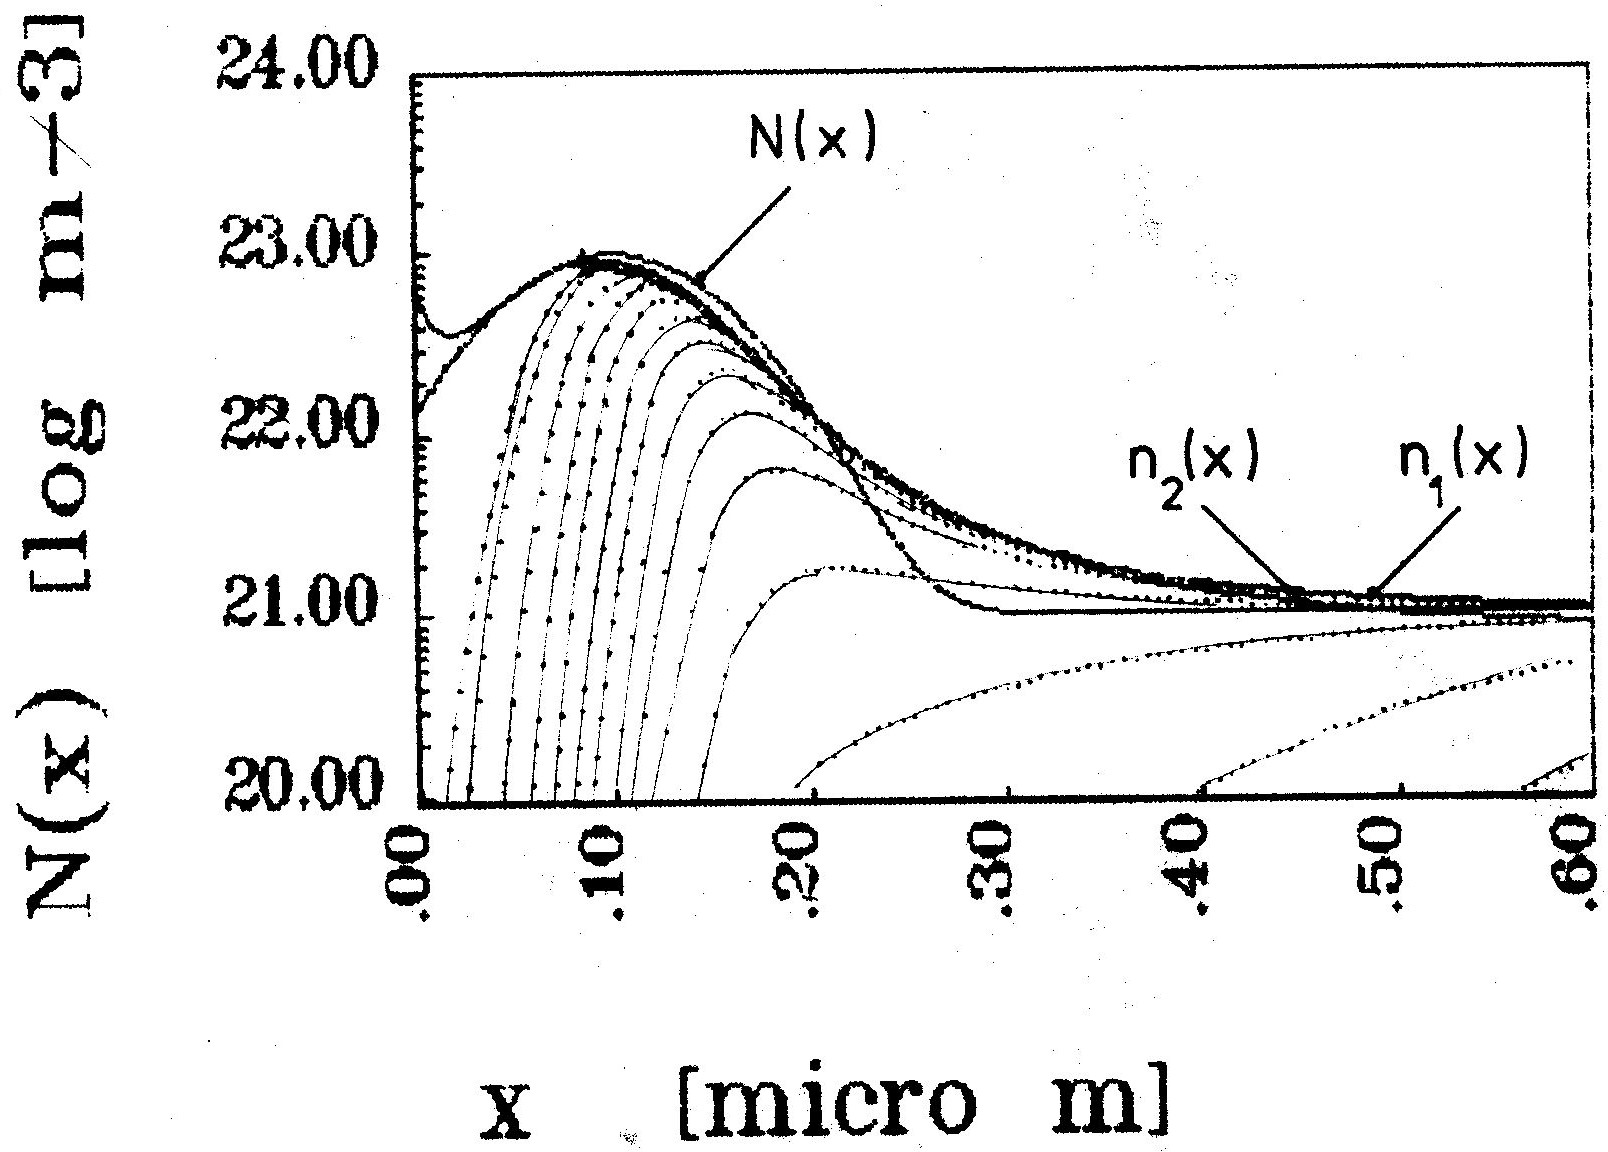
\includegraphics{Figures/fig-4-4.eps}
  \caption[Gaussian simulated impurity concentration
    distribution]{Admixture concentration profile $N(x)$ simulated by
    Gaussian distribution with parameters $R_{p}=0.1\mu m$, $\Delta
    R_{p}=0.05\mu m$, $N_{\max}=1.0\times 10^{23} m^{-3}$,
    $N_{bulk}=1.0\times10^{21}m^{-3}$; majority carrier progression
    charge $n_{1}(x)$ and the $n_{2}(x)$ waveform obtained from the
    theoretical C-V dependence. The dotted lines show the depletion of
    the MOS structure.}\label{fig:4.4}
\end{figure}
% OBR24.BIT

\begin{figure}[h!]\centering
  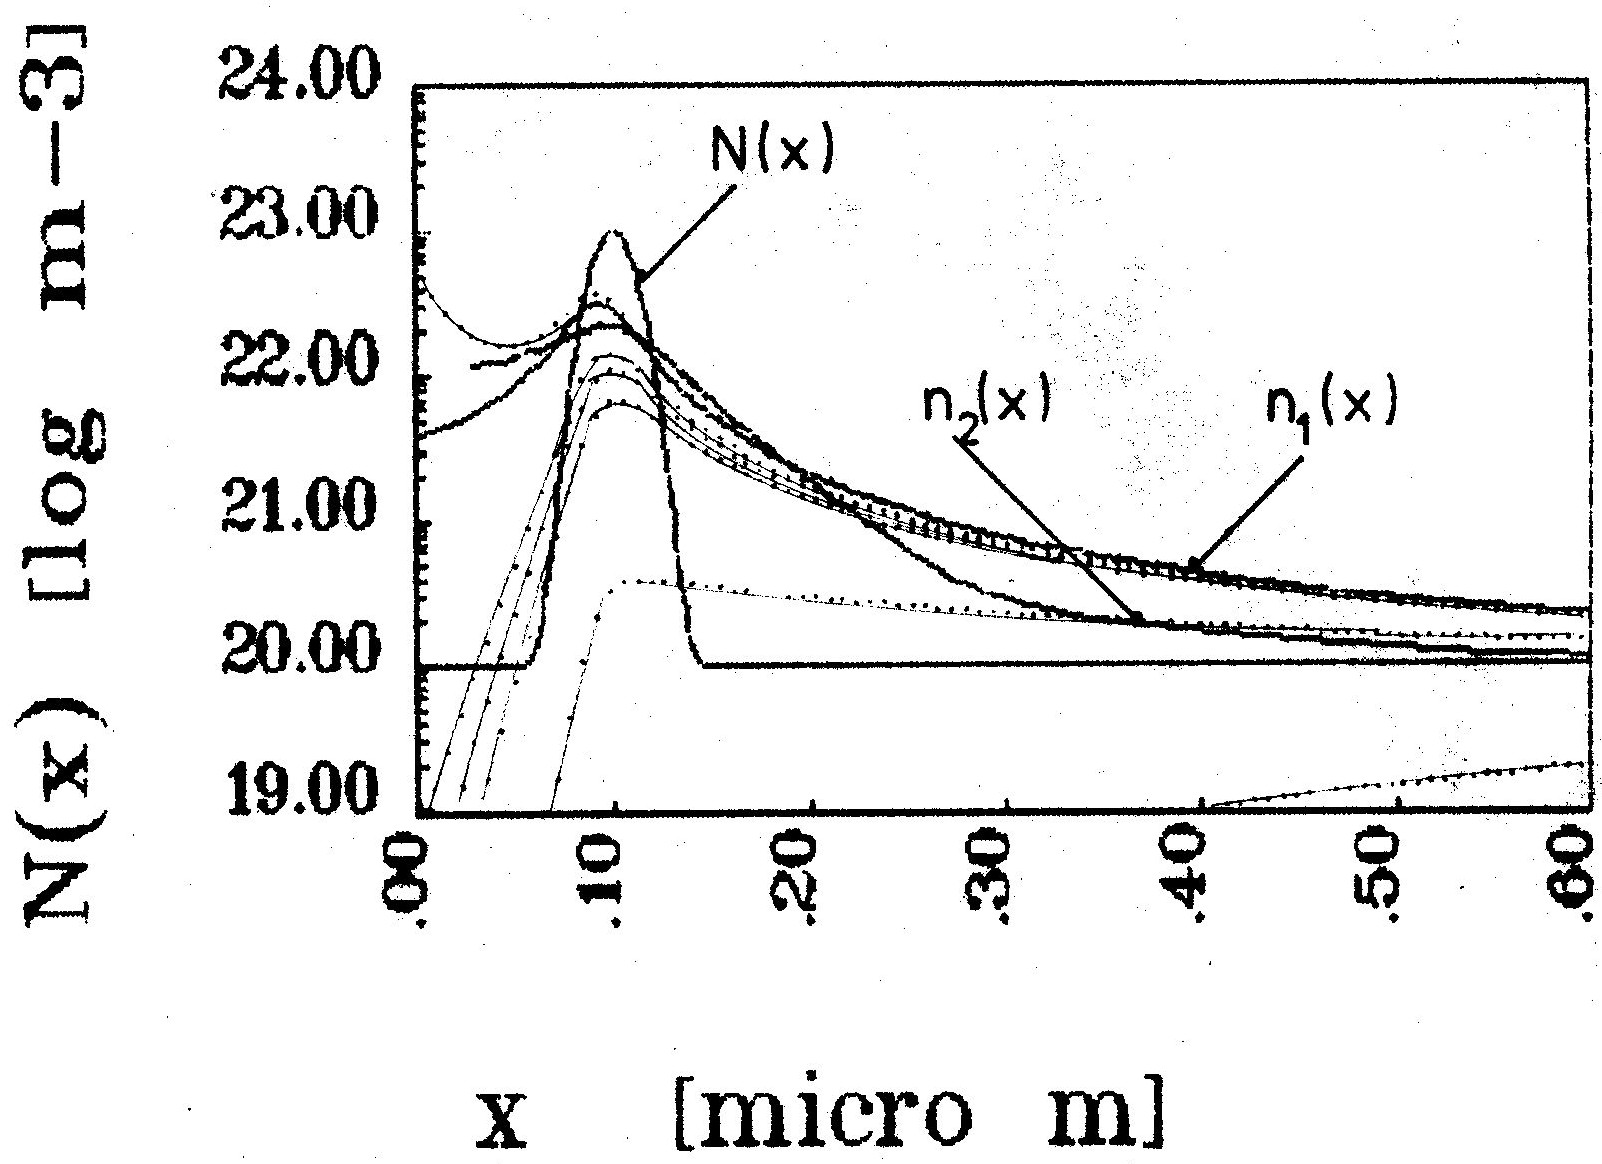
\includegraphics{Figures/fig-4-5.eps}
  \caption[Gaussian-simulated impurity concentration profile
    distribution]{Gaussian simulated $N(x)$ admixture concentration
    profile Gaussian distribution with parameters $R_{p}=0.1\mu m$,
    $\Delta R_{p}=0.01\mu m$, $N_{\max}=1.0\times10^{23}m^{-3}$,
    $N_{bulk}=1.0\times10^{21}m^{-3}$; majority carrier waveform
    charge $n_{1}(x)$ and the $n_{2}(x)$ waveform obtained from the
    theoretical C-V dependence. The dotted lines show the depletion of
    the MOS structure.}\label{fig:4.5}
\end{figure}
%OBR25.BIT

\par Further analysis of the approximations used in the calculation of
concentration profiles could focus on finding an exact bound validity
of these approximations, but from a systematic point of view it would
be to address this issue, it would be more efficient to take an
approach that to which the following remark refers.

\par\emph{Note.} Using capacitance measurements, it would be possible
to determine $N(x)$ waveform exactly without using the approximations
given in previous articles.  In the work of~\cite{4.4} Appendix A it
is indicated a procedure for calculating the electric potential in a
semiconductor, which is a function of of the distance (from the
semiconductor surface to the depth) and the gate voltage.  Derivation
of Poisson's equation~\ref{eq:1.2} by $V_{g}$ gives a third-order
partial differential equation that accurately describes C-V dependence
measurement experiment

\begin{equation}\label{eq:4.13}
  \frac{\delta^{3}\varphi}{\delta x^{2}\delta V_{g}} = {\frac{1}{L_{D}^{2}}}\ {e^{\beta\varphi}}\ {\frac{\delta\varphi}{\delta V_{g}}}
\end{equation}

By solving it using appropriate boundary conditions, it would be
possible to obtain a surface $\varphi(x,V_{g})$ from which to compute
$N(x)$ only one line $\varphi(x)\rvert_{V_{g}}$

\begin{equation}\label{eq:4.14}
  N(x) = N_{bulk}\ e^{\beta\varphi}-\frac{\epsilon}{q}\frac{\delta^{2}\varphi}{\delta x^{2}}
\end{equation}

(todo: check equation 4.14 in ref 4.4)

The authors of paper~\cite{4.4} did not develop this method further,
for reasons the difficulty of quantifying the second derivative in
equation~\ref{eq:4.14}.


\section{Determination of $Si-SiO_{2}$ interface traps density.}\label{sec:4.2}

We characterize the quality of the $Si-SiO_{2}$ interface by the trap
density of the interface $(D_{it})$, which is a consequence of the
thermal oxidation mechanism of silicon, which produces a region of
non-stoichiometric composition. This density can be evaluated by the
following two procedures:

\begin{enumerate}
\item Comparison of measured high frequency C-V dependence
  $C_{mos}^{HF}(V_{g})$ and the measured low-frequency C-V dependence
  $C_{mos}^{LF}(V_{g})$. Evaluation of $D_{it}$ by comparison of the
  above dependencies is based on the assumption that the dependence
  $C_{mos}^{HF}(V_{g})$ is measured by a sufficiently high VF signal,
  which causes the capacitance to be unaffected by interface traps
  $Si-SiO_{2}$.
\item Comparison of the measured dependence of $C_{mos}^{LF}(V_{g})$
  and the theoretical low-frequency C-V dependence, which we denote
  $C_{mos}^{TLF}(V_{g})$.  In this case, based on the known
  concentration profile of the interfering impurities in the
  subsurface region of the semiconductor to calculate the dependence
  $C_{mos}^{TLF}(V_{g})$ by solving the Poisson equation.
\end{enumerate}

To evaluate $D_{it}$, we used both methods, the implementation of
which in we will detail in the following.

\subsection{Comparison of high and low frequency C-V dependence.}\label{sec:4.2.1}

In this case, we use the frequency dependence of the capacitance of
the MOS structure and $D_{it}$ is determined from the comparison of
$C_{mos}^{HF}(V_{g})$ and $C_{mos}^{LF}(V_{g})$. The necessary
theoretical basis can be found for example, in~\cite{I.1}.  To
determine $C_{mos}^{HF}(V_{g})$ and $C_{mos}^{LF}(V_{g})$, it is
convenient to use the Q-C method~\{cite{3.4, 3.6, 3.7,3.8}, which
allows simultaneous determination of both dependencies, but the use of
the standard methods for determining $C_{mos}^{HF}(V_{g})$ and
$C_{mos}^{LF}(V_{g})$ is also possible.

\begin{figure}[h!]\centering
  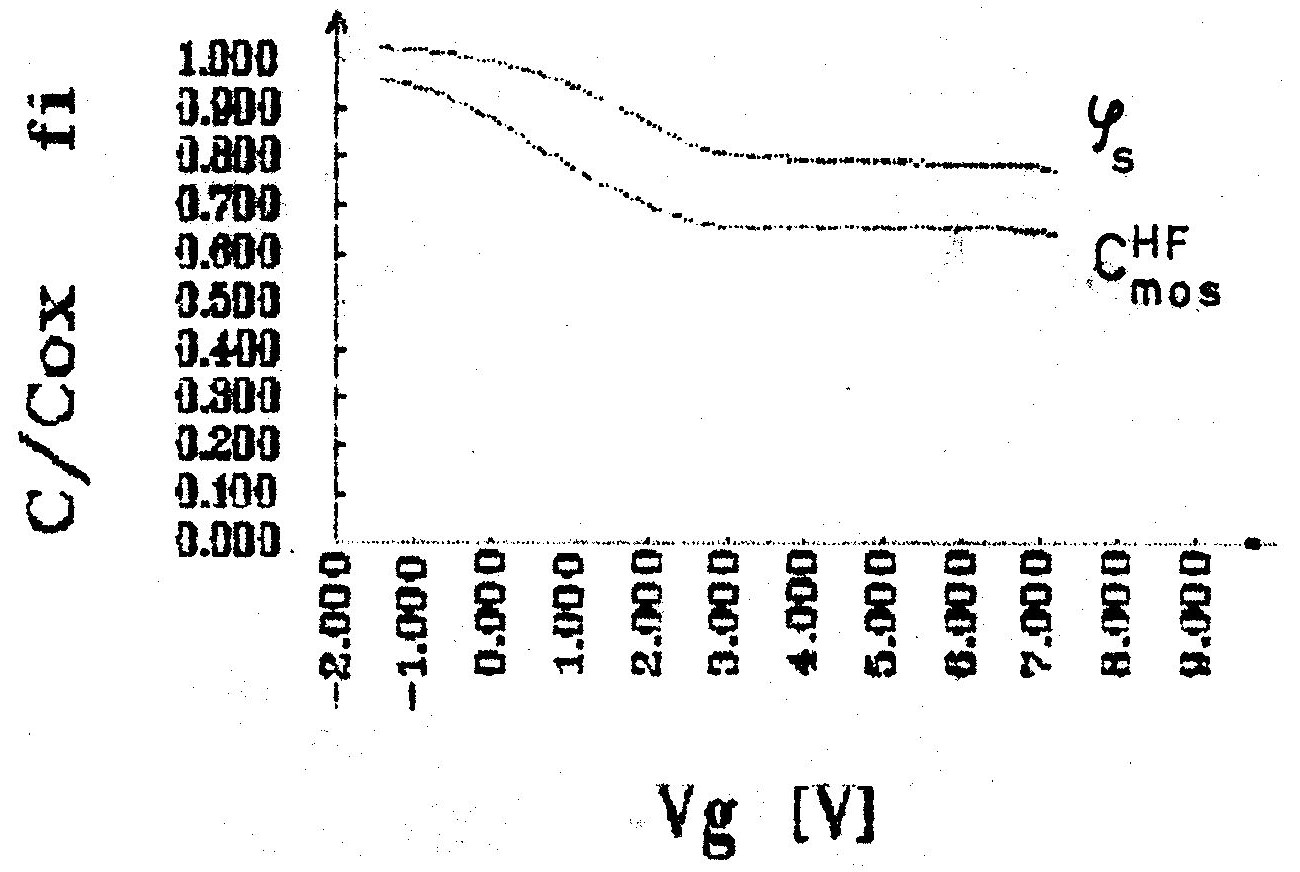
\includegraphics{Figures/fig-4-6.eps}
  \caption[VF C-V dependence of $C_{mos}^{HF}(V_{g})$ and waveform of
    the surface potential $\varphi_{s}(V_{g})$ of the MOS structure
    obtained using the Q-C method]{VF C-V dependence of
    $C_{mos}^{HF}(V_{g})$ normalized to the oxide capacitance and the
    normalized surface potential of the $\varphi_{s}(V_{g})$ structure
    of MOS obtained by Q-C method. The surface potential waveform is
    normalized by the relationship
    $1-\frac{\varphi_{s}}{\varphi_{norm}}$, kde
    $\varphi_{norm}=3.33$.}\label{fig:4.6}
\end{figure}
% OBR15.BIT

In figure~\ref{fig:4.6} the measured values of $C_{mos}^{HF}(V_{g})$
and surface potential $\varphi_{s}$ of the MOS structure, determined
by Q-C method. The curves are shown in Figure~\ref{fig:4.7}
$C_{mos}^{HF}(V_{g})$ and $C_{mos}^{LF}(V_{g})$, which we use for
calculate $D_{it}$ according to the following equation~\{cite{4.15}

\begin{equation}\label{eq:4.15}
  D_{it} = {\frac{1}{q}} {\left[\frac{C_{mos}^{LF}}{1-\cfrac{C_{mos}^{LF}}{C_{ox}}}-\frac{C_{mos}^{HF}}{1-\cfrac{C_{mos}^{HF}}{C_{ox}}}\right]}
\end{equation}
% was (4.14) in origin

\begin{figure}[h!]\centering
  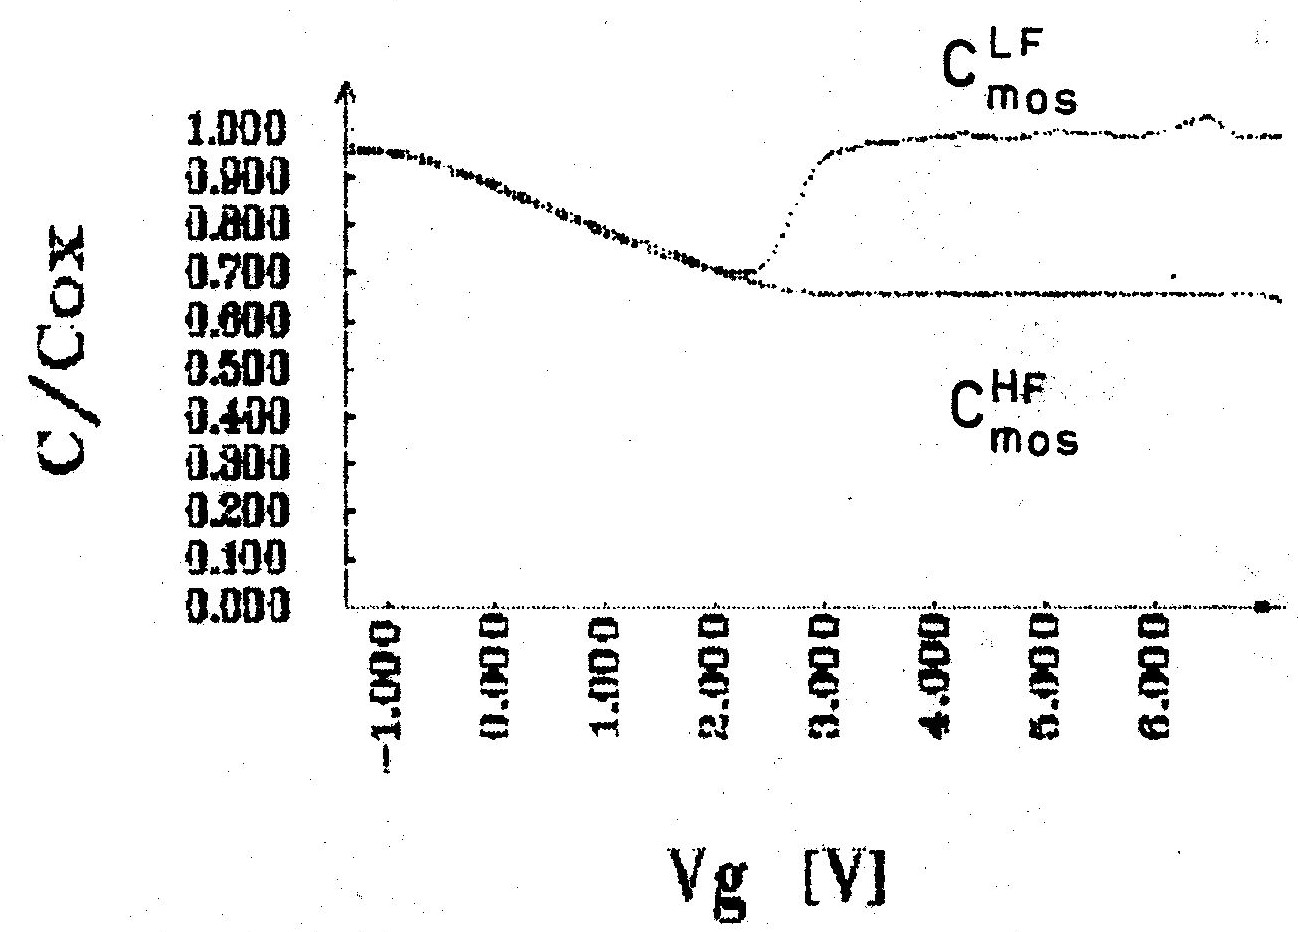
\includegraphics{Figures/fig-4-7.eps}
  \caption[VF C-V dependence $C_{mos}^{HF} (V_{g})$ and LF C-V
    dependence $C_{mos}^{LF} (V_{g})$ of the MOS structure normalized
    to the oxide capacitance, obtained using the Q-C method]{LF C-V
    dependence of $C_{mos}^{HF} (V_{g})$ and LF C-V dependence of
    $C_{mos}^{LF} (V_{g})$ structures of MOS normalized to the oxide
    capacitance, obtained using the Q-C method.  LF C-V dependence is
    calculated by deriving the surface potential (shown in
    Figure~\ref{fig:4.6}) according to the
    relation~\ref{eq:3.2}.}\label{fig:4.7}
\end{figure}
% OBR12.BIT

\par The position of the Fermi level in the forbidden band for the
calculated values $D_{it}$ are determined using the values of the
surface potential $\varphi_{s}$ and the distance of the Fermi surface
from the intrinsic Fermi surface $\varphi_{f}$. The surface potential
$\varphi_{s} (V_{g})$ is obtained either directly using the Q-C method
or by integration quasi-static C-V dependence using the Berglund
integral. In both both cases, we obtain the waveforms
$\varphi_{s} (V_{g})$, which are shifted in direction of the
$y$-axis. In the case of the Q-C method, this is a constant
$\varphi_{s0}$, which represents the surface potential if at the gate
of the MOS structure is not connected and in the case of the
quasi-static C-V method, the displacement represents the integration
constant. For both cases we can calculate the shift dependence
$\varphi_{s} (V_{g})$ using the procedure given in
Appendix~\ref{app:AppendixG}.

\begin{figure}[h!]\centering
  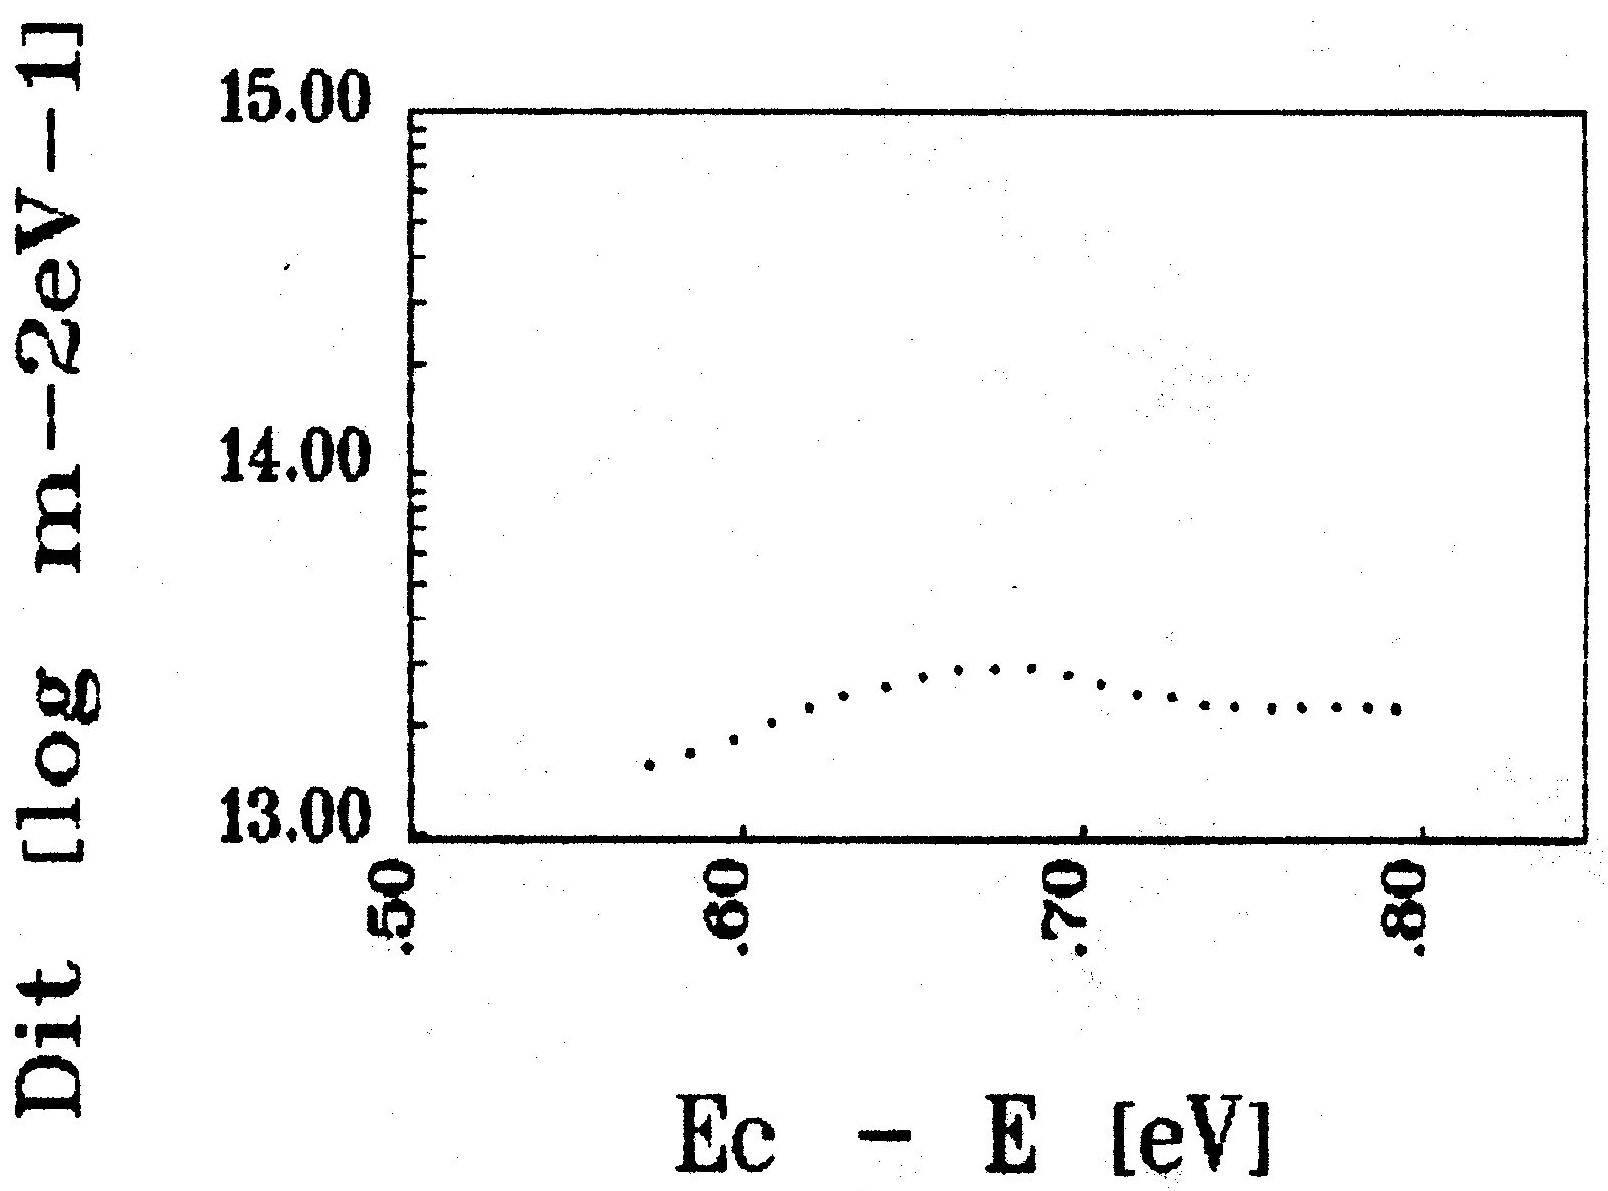
\includegraphics{Figures/fig-4-8.eps}
  \caption[Dependence of $D_{it}$ on the position in the forbidden
    band of the semiconductor of a P-type semiconductor, determined
    from the comparison of $C_{mos}^{HF} (V_{g})$ and
    $C_{mos}^{LF} (V_{g})$]{The dependence of $D_{it}$ on the position
    in the forbidden band of a P-type semiconductor, determined from a
    comparison of $C_{mos}^{HF} (V_{g})$ and $C_{mos}^{LF} (V_{g})$,
    which are shown in obrázku~\ref{fig:4.7}.}\label{fig:4.8}
\end{figure}
% OBR14.BIT

The value of the potential $\varphi_{f}$ is determined using the relation

\begin{equation}\label{eq:4.16}
  \varphi_{f} = \pm \frac{kT}{g} \ln{\frac{N_{b}}{n_{i}}}
\end{equation}

, where we assume knowledge of the substrate concentration
$N_{b}$. Potential $\varphi_{f}$ has a positive sign for a P-type
semiconductor. If for surface potential $\varphi_{s}$ we choose the
same orientation as for $\varphi_{f}$, the energy position of the
interface traps in the forbidden band is then determined using the
following relation

\begin{equation}\label{eq:4.17}
  E_{c} - E = 0.56 + \varphi_{s} + \varphi_{f}
\end{equation}

, where $0.56$ represents the distance of the lower edge of the
conductivity band $(E_{c})$ from the intrinsic Fermi level. Run
$D_{it}$ as a function of position in the forbidden band is shown
in Figure~\ref{fig:4.8}.

\subsection{Comparison of experimental and theoretical quasi-static CV dependence.}\label{sec:4.2.2}

To calculate $D_{it}$ using this method, it is necessary to know the
waveform the concentration profile of the interfering impurities in
the subsurface of the semiconductor $N(x)$ in order to calculate
$C_{mos}^{TLF}(V_{g})$. The theoretical dependence of
$C_{mos}^{TLF}(V_{g})$ of the MOS structure is calculated by the
numerical procedure described in Appendix~\ref{app:AppendixA}.  The
use of numerical methods in this case is necessary because the
analytical solution of the Poisson equation is not possible for the
general $N(x)$ concentration distribution.  For numerical solution of
the Poisson equation, we also calculate the dependence of the surface
potential on the gate voltage $\varphi_{s}(V_{g})$, which we use to
determine the position of the calculated interface trap density in the
forbidden band of the semiconductor.  Because during the numerical
calculation we do not take into account the breakdown charges in the
oxide layer and at the interface $Si-SiO_{2}$ both theoretically
determined dependencies $\varphi_{s}(V_{g})$ and
$C_{mos}^{TLF}(V_{g})$ will both be shifted with respect to the
measured quasi-static C-V dependence by the value of $V_{FB}$. To
shift the above dependencies we also need to know the value of
$V_{FB}$.

\par To calculate $D_{it}$ we therefore use $C_{mos}^{TLF}(V_{g})$,
which is not burdened by the trapping capacity of the $Si-SiO_{2}$
interface. At Figure~\ref{fig:4.9} the measured and theoretical LF C-V
dependence, which we use below to evaluate $D_{it}$ according to the
relation

\begin{equation}\label{eq:4.18}
  D_{it} = \frac{1}{q} \left[\cfrac{C_{mos}^{LF}}{1-\cfrac{C_{mos}^{LF}}{C_{ox}}}-\cfrac{C_{mos}^{TLF}}{1-\cfrac{C_{mos}^{TLF}}{C_{ox}}}\right]
\end{equation}

Figure~\ref{fig:4.10} shows the trap density of the interface as a
function of position in the forbidden band of the semiconductor
determined by in the above manner.  The disadvantage of the described
method lies in the time of calculating the theoretical low-frequency
C-V dependence. Although the comparison of theoretical and
experimental low-frequency C-V dependence gives values of $D_{it}$ in
a larger region of the forbidden band, for the evaluation of the areal
distribution $D_{it}$ on a silicon wafer, we have used the following
procedure due to time constraints described in section~\ref{sec:4.2.1}

\begin{figure}[h!]\centering
  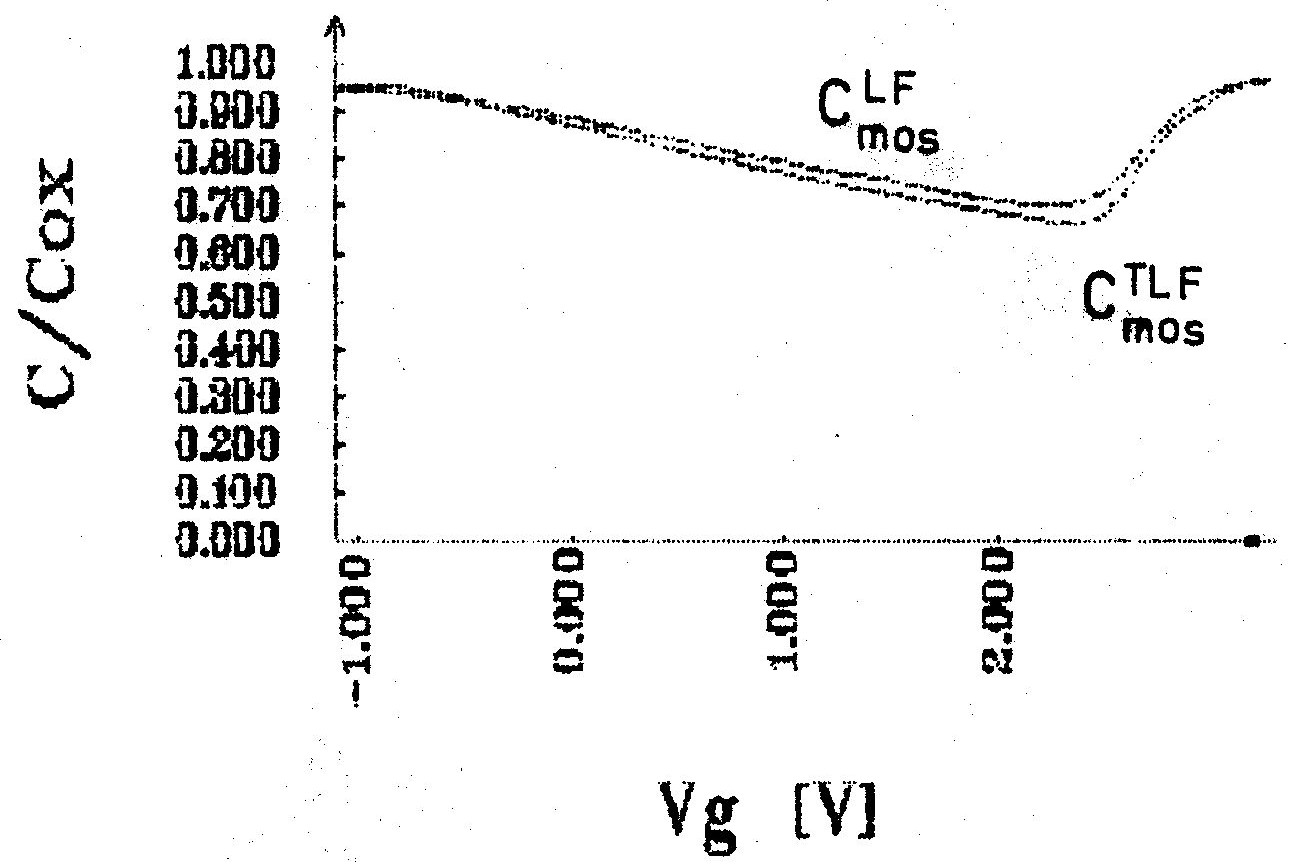
\includegraphics{Figures/fig-4-9.eps}
  \caption[Theoretical LF C-V dependence and measured LF C-V
    dependence]{Theoretical LF C-V dependence and measured LF C-V
    dependence MOS structures normalized to oxide
    capacitance.}\label{fig:4.9}
\end{figure}
% OBR11.BIT

\begin{figure}[h!]\centering
  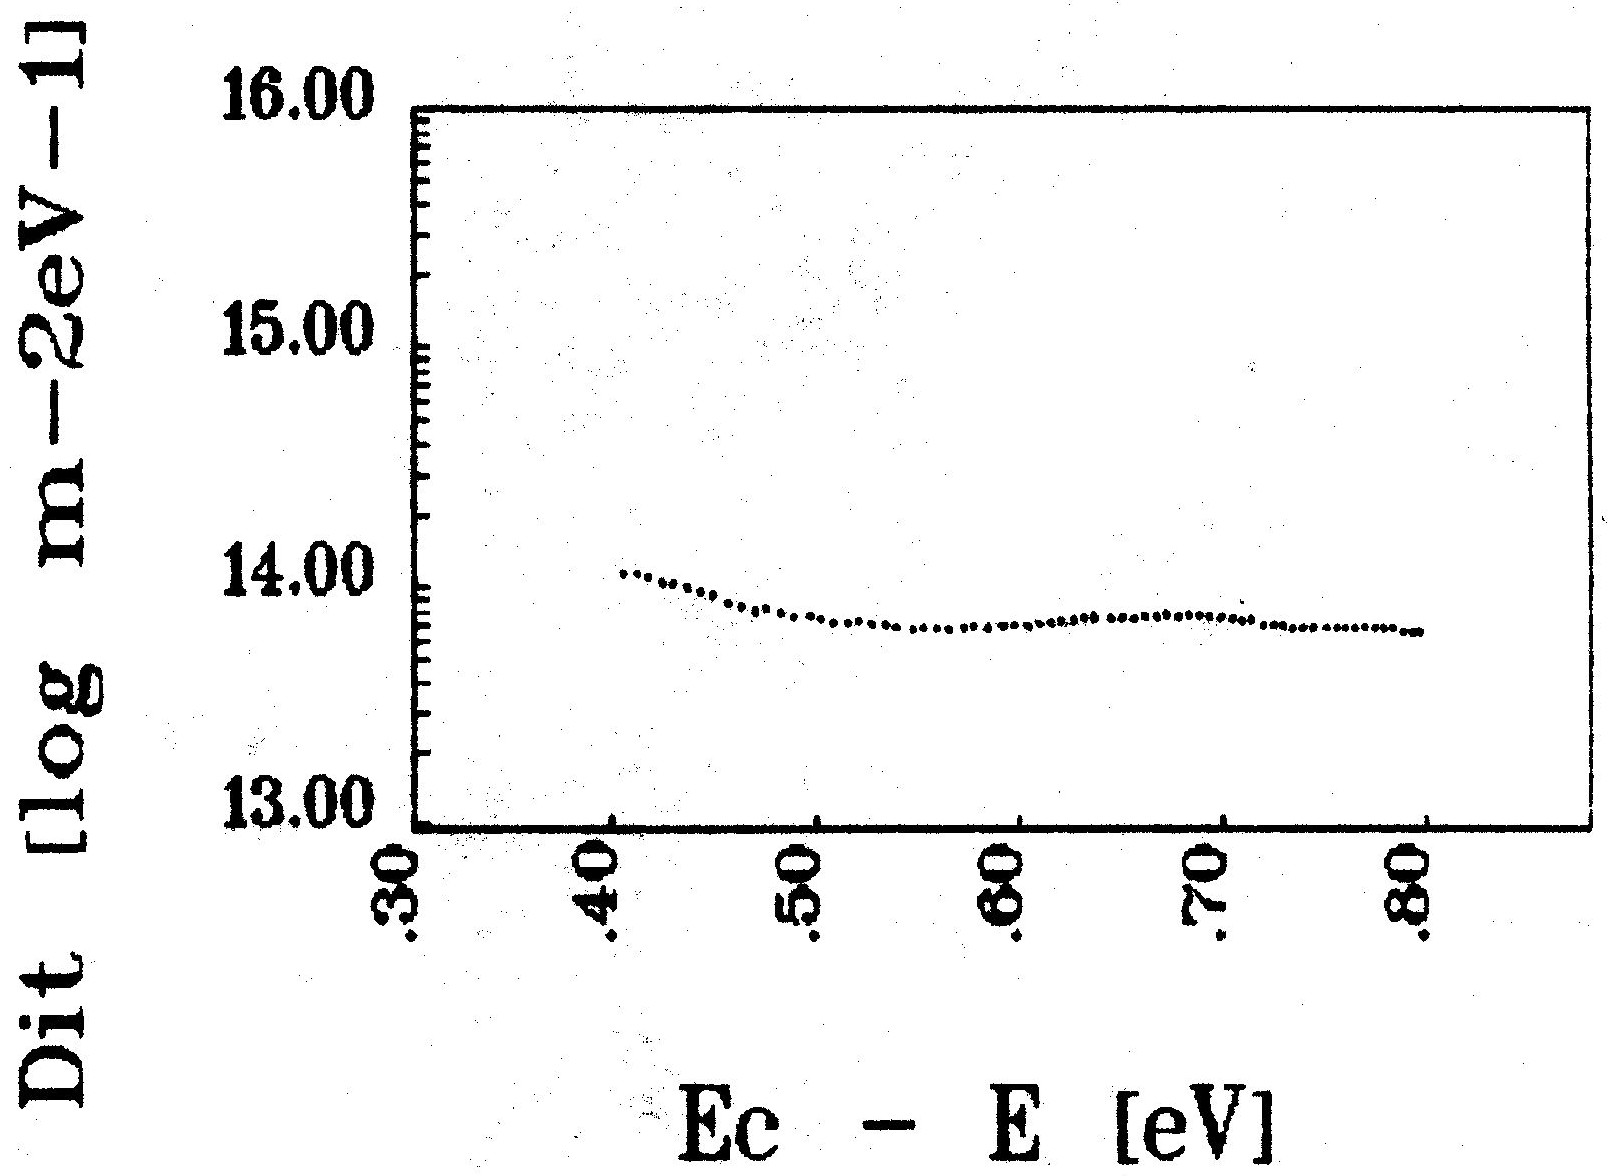
\includegraphics{Figures/fig-4-10.eps}
  \caption[Dependence of $D_{it}$ on the position in the forbidden
    band of the semiconductor determined from the comparison of
    $C_{mos}^{TLF}(V_{g})$ and $C_{mos}^{LF}(V_{g})$]{$D_{it}$
    dependence on the position in the forbidden band of a P-type
    semiconductor, determined from a comparison of
    $C_{mos}^{TLF}(V_{g})$ and $C_{mos}^{LF}(V_{g})$, which are shown
    in Figure~\ref{fig:4.9}.}\label{fig:4.10}
\end{figure}
% OBR13.BIT


\begin{thebibliography}{}
\bibitem[4.1]{4.1} Lehovec K.: Solid St\.  Electron.  27 (1984)
  s.1907.
\bibitem[4.2]{4.2} Wu Chung P., Douglas E.C., Mueller C.W.: IEEE
  Trans.\ on electron.\ dev. 22 (1975) s.319.
\bibitem[4.3]{4.3} Kroemer H., Chien W.: Solid St.\ Electron. 24
  (1981) s.655.
\bibitem[4.4]{4.4} Baccarani G., Rudan M., Maes H., Vandervorst W.,
  Van Overstraeten R.: Solid St\. Electron. 23 (1980) s. 65.
\bibitem[4.5]{4.5} Botka V., Csabay O., Artz P., Beyer A.: 3rd
  Scientific Conference EF SVŠT Elektrotechnika '90, EF SVŠT
  Bratislava, 1990 s.73.
\bibitem[4.6]{4.6} Kinder R.: Contribution to the investigation of
  concentrating profiles of implanted layers. Candidate's
  dissertation. EF SVŠT Bratislava 1984.
\bibitem[4.7]{4.7} Lin S.T., Reuter J.: Solid St.\ Electron. 26 (1983)
  s.343.
\bibitem[4.8]{4.8} Ziegler K., Klausmann E.: Solid St.\ Electron. 18
  (1975) s.189.
\bibitem[4.9]{4.9} Jindal R.P., Warner R.M. Jr.: IEEE Trans.\ on
  electron.\ dev. 28 (1981) s.348.
\bibitem[4.10]{4.10} Jindal R.P.: Solid St.\ Electron. 26 (1983)
  s.1005.
\bibitem[4.11]{4.11} Warner R.M. Jr., Jindal R.P.: Solid
  St.\ Electron. 26 (1983) s.335.
\bibitem[4.12]{4.12} Balland B., Remaki B., Marchand J.J.:
  J. Phys. E. Sci. Instrum. 21 (1988) s.559.
\bibitem[4.13]{4.13} Csabay O., Botka V.: 5th national conference
  Microelectronics 1989, House of Techniques CSVTS Bratislava, 1989
  p.58.
\bibitem[4.14]{4.14} Zsalkovics G.: Determination of the concentration
  profile of the implanted layer from capacitance
  measurements. Diploma thesis, Department Microelectronics, EF SVŠT,
  Bratislava 1988.
\bibitem[4.15]{4.15} Zohta Y.: Solid St.\ Electron. 17 (1974), s.1299.
\bibitem[4.16]{4.16} Kennedy O.P., Murley P.C., Kleinfelder W.: IBM
  J. Res. Dev. 12 (1968) p.399.
\bibitem[4.17]{4.17} Nishida V.: IEEE Trans. Electron. Dev. ED-26
  (1979) s.1081.
\bibitem[4.18]{4.18} Johnson W.C., Panousis P.T.: IEEE
  Trans. Electron. Dev. ED-18 (1971) s.965.
\bibitem[4.19]{4.19} Isaacson E., Keller H.B.: Analysis of numerical
  memethods.  John Wiley and Sons. New York.
\bibitem[4.20]{4.20} Vitásek E.: Numerické metody. SNTL, Praha 1987.
\bibitem[4.21]{4.21} Hamming R.W.: Digital filters. Prentice Hall.
\bibitem[4.22]{4.22} Beyer A., Tolonics J.: Physik der
  Halbleiteroberflbche 17 (1986) s.91.
\end{thebibliography}
 
% Chapter 5

\chapter{Pracovisko pre automatizovaný zber dát.} % Main chapter title

\label{Chapter5} % For referencing the chapter elsewhere, use \ref{Chapter1} 

\lhead{Chapter 5. \emph{Pracovisko pre automatizovaný zber dát}} % This is for the header on each page - perhaps a shortened title

Na popisovanom pracovisku možno automaticky merať vysokofrekvenčnú a
nízkofrekvenčnú kapacitu štruktúry MOS. Na obrázku \ref{fig:5.1} je
zobrazené blokové zapojenie prístrojov, pomocou ktorých sú jednotlivé
metódy realizované.

\begin{figure}[h!]\centering
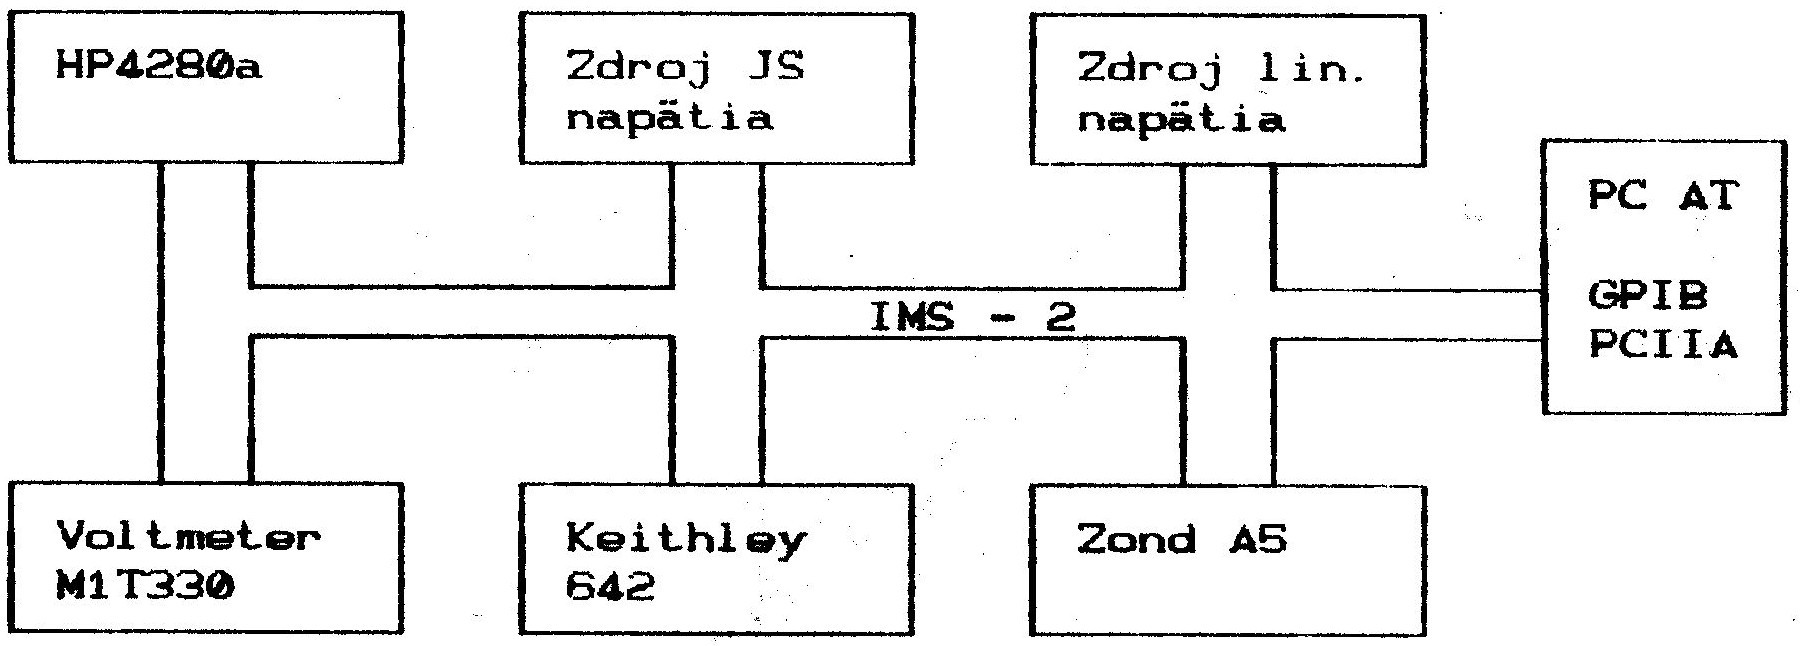
\includegraphics{Figures/fig-5-1.eps}
\captionsetup{justification=raggedright, singlelinecheck=false}
\caption[Bloková schéma zapojenia prístrojov automatizovaného
  pracoviska]{Bloková schéma zapojenia prístrojov automatizovaného
  pracoviska pre určovanie plošného rozloženia parametrov štruktúr MOS
  s nehomogénnou dotáciou substrátu.}
\label{fig:5.1}
\end{figure}

Riadiacim počítačom meraní je osobný počítač PC AT vybavený
interfejsom IMS-2 (norma IEEE 488) firmy National Instruments model
GPIB-PCIIA, ktorý pracuje ako riadič zbernice IMS-2. Všetky pripojené
prístroje sú vybavené interfejsom IMS-2, pomocou ktorého ich možno
diaľkovo ovládať a zberať namerané údaje. Okrem profesionálnych
meracích prístrojov HP4280a a Keithley 642 boli v experimente použité
zdroje jednosmerného napätia a zdroj lineárne narastajúceho napätia
postavené na Katedre mikroelektroniky. Voltmeter M1T330 je výrobkom
Metry Blansko a krokovacie hrotové zariadenie Zond A5 bolo dovezené zo
Sovietskeho Zväzu. Posledne spomínané zariadenie neobsahuje štandardne
interfejs IMS-2 a bolo dodatočne vybavené modulom IMS-2 vlastnej
konštrukcie \cite{5.1}.

Ďalším novým prvkom našej realizácie pracoviska pre meranie štruktúr
MOS je možnosť automatického zberu dát po celej kremíkovej doske a ich
uloženie do diskového súboru pre následovné spracovanie. Programové
vybavenie pracoviska možno rozdeliť na programy (1) zberu dát (2)
spracovania dát (3) zobrazenia vysledkov a (4) pomocné
programy. Programy zberu dát umožňujú meranie C-V závislosti v
ľubovoľnom počte bodov kremíkovej dosky, ktorých pozície sú voliteľné
a sú definované operátorom.

Dôležitým momentom pri realizácii programov zberu dát bolo
zabezpečenie proti strate nameraných dát v dôsledku výskytu ľubovolnej
chyby (napr. výpadku napätia), alebo v prípade nutnosti prerušiť
meranie. Pretože trvanie zberu dát na kremíkovej doske s 300
štruktúrami sa pohybuje od 0.5 do 12 hodín v závislosti od
požadovaného druhu merania, bolo potrebné programovo zabezpečiť (1)
možnosť prerušenia merania operátorom v ľubovoľnom bode (2) možnosť
opätovného reštartovania zberu dát v bode, kde bol zber dát
prerušený. Zabezpečenie uchovania nameraných dát v prípade výskytu
chyby bolo realizované následovným spôsobom. Namerané dáta sú naraz
zapisované do diskového súboru vždy po ukončení merania na každej
štruktúre. Túto dátovu jednotku budeme v ďalsom označovat záznam. To
znamená, že k poškodeniu štruktúry dát môže prísť len v prípade
výskytu chyby v priebehu krátkeho časového úseku (rádove desiatky ms),
čím ale prichádza len k strate posledného záznamu. Pre tento prípad je
k dispozícii pomocný program, ktorý zkráti dátový súbor na požadované
množstvo záznamov, čím obnoví kompaktnosť súboru a umožní
reštartovanie zberu dát. Týmto spôsobom možno skrátiť dátovy súbor o
chybne namerané dáta aj po prerušení zberu dát operátorom, ak bola
zistená nejaká závada v priebehu merania. Zároveň je k dispozícii
pomocný program, ktorý umožňuje prepísanie ľubovolného počtu záznamov
dátového súboru. Užitočnosť tohto programu vysvetlíme v následovnom
príklade.

Predstavme si, že v priebehu zberu dát došlo (napr.dôsledkom vplyvov
okolia) ku chybe, ktorá trvala krátky časový úsek, čo spôsobilo, že
časť záznamov dátového súboru obsahuje chybné dáta. Príkladom môže byť
nedokonalosť kontaktu hrotu s meranou vzorkou spôsobená vibráciami. To
sa často zistí až pri vyhodnocovaní merania, prípadne pri zobrazení
výsledkov. Po určení pozícií štruktúr na testovanej kremíkovej doske,
v ktorých sme namerali chybné údaje, môžeme v týchto bodoch meranie
zopakovať a pomocným programom prepísať záznamy v pôvodnom dátovom
súbore.

Uvedeným spôsobom boli realizované programy zberu dát pre HF C-V,
kvázistaticku C-V metódu, meranie kapacity oxidovej vrstvy a metódu
konštantnej šírky oblasti priestorového náboja. Takto sme ale nemohli
automatizovať Q-C metódu, pretože použitý interfejs prístroja Keithley
642 neumožňuje diaľkové ovládanie skratovania vstupných svoriek
meracieho prístroja, čím nemožno automatizovať vynulovanie náboja v
spoločnom bode zapojenia kondenzátorov, ktorý sa tam dostane vplyvom
zvodových prúdov.

Pre pohodlnú manipuláciu s dátovými súbormi bola zvolená následovná
koncepcia pomenovania dátovych súborov. Pomenovanie súboru v operačnom
systéme MS DOS pozostáva z mena súboru a prípony.  Meno súboru
predstavuje v našom prípade názov meranej kremíkovej dosky a prípona
označuje druh dát, ktoré súbor obsahuje. Principiálne možno rozdeliť
uvedené dátove súbory na dva typy podľa dát, ktoré obsahujú jednotlivé
záznamy. Môže to byť funkčná závislosť alebo parameter. Ak sa jedná o
funkčnú závislosť, potom prvý záznam v dátovom súbore obsahuje počet
bodov, v ktorých bola funkčná závislosť zosnímaná a hodnoty nezávislej
premennej. Ďalšie záznamy obsahujú pozíciu štruktúry na kremíkovej
doske, vyjadrenú dvoma celými číslami (X,Y), počet bodov a funkčné
hodnoty.  Opakujúca sa informácia o počte bodov funkčnej závislosti
nie je redundantná, pretože v prípade neúspešnosti merania
(napr.prieraz) na štruktúre (X,Y) obsahuje číslo -1, ktoré oznamuje
neprítomnosť funkčných hodnôt v zázname. Príkladom môže byť HF C-V
závislosť. Prvý záznam obsahuje počet meraní kapacity na jednej
štruktúre a hodnoty napätia hradla. Ďalšie záznamy obsahujú pozíciu
štruktúry (X,Y), počet bodov a hodnoty kapacity zodpovedajúce
hradlovým napätiam z prvého záznamu. Súbory druhého typu pozostávajú
len zo záznamov, ktoré obsahujú pozície štruktúry (X,Y) a hodnotu
parametra. Ako príklad uvedieme dátový súbor, ktorý obsahuje kapacity
oxidovej vrstvy štruktúr MOS. Pretože sa jedná o rozsiahle dátové
súbory bola zvolená binárna forma záznamu.  Celočíselné hodnoty majú
dĺžku 2 bajty a čísla s pohyblivou desatinnou čiarkou zaberajú 4
bajty.

Pre prípad, že by bol potrebný dátovy súbor, obsahujúci dáta vo forme
ASCII, je k dispozícii pomocný program, ktorý po zadaní pozície
štruktúry (X,Y) vytvorí tento dátový súbor a zapíše do neho dáta,
ktoré obsahuje záznam s pozíciou (X,Y). Ak sa jedná o funkčnú
závislosť, zapíše do výstupného súboru vo forme ASCII aj hodnoty
nezávislej premennej.

\section{Meranie HF C-V závislostí.}\label{sec:5.1}

HF C-V závislosť štruktúry MOS meriame pomocou prístroja HP4280a,
ktorý určuje zároveň kapacitu a vodivosť meranej vzorky na základe
fázového posunu madzi HF napäťovým signálom (1MHz,30mV) a meraným
prúdom. Prístroj HP4280a je vybavený vlastným procesorom, ktorý riadi
jeho vnútorné funkcie a operátorovi poskytuje komfortné ovládanie. Pre
meranie HF C-V závislosti musíme nastaviť požadovaný interval napätia,
v ktorom sa má merať kapacita (Vstart, Vstop) a napäťový krok Vstep,
ktorým sa bude jednosmerné napätie meniť. Časové pomery merania sa
určujú ďalšími dvoma parametrami. Thold určuje čas, počas ktorého bude
na meranej vzorke pripojené napätie Vstart pred začiatkom
merania. Tento čas je potrebný na ustálenie prechodových javov, v
prípade že ich nechceme merať. Parameter Tdelay určuje dobu pozdržania
merania po vykonaní napäťového kroku.

Pre automatizované meranie štruktúr sme zvolili najvýkonnejší mód
prístroja HP4280a, v ktorom podľa vopred nastavených parametrov
automaticky vykoná celé meranie a namerané dáta uloží do vnútornej
pamäte.  Prenos dát z prístroja HP4280a do riadiaceho počítača sa
vykoná v binárnej forme, čím nestrácame čas konverziou medzi binárnou
formou a formou ASCII a zároveň binárna forma predstavuje menšie
množstvo prenášaných bajtov. Ukončenie merania a pripravenosť na
prenos dát signalizuje prístroj HP4280a nastavením signálu SRQ
(Service Request) na zbernici IMS-2, čím je synchronizovaná jeho
činnosť s riadiacim počítačom.  Tu možno spomenúť užitočnú vlastnosť
interfejsu GPIB-PCIIA \cite{5.2}, ktorý po detekovaní signálu SRQ môže
automaticky vykonať sériové hlásenie prístrojov (Serial Poll) a po
nájdení prístroja, ktorý žiada o obsluhu uložiť jeho stavové slovo do
internej pamäte. Tým je vodič SRQ zbernice IMS-2 uvolnený a interfejs
GPIB-PCIIA môže reagovať na žiadosť o obsluhu od ďalších
prístrojov. Ak riadiaci program požaduje stavové slovo prístroja,
ktorý žiadal o obsluhu, interfejs GPIB-PCIIA ho vydá zo svojej
internej pamäte.

Použitím automatického riadenia merania a binárneho prenosu dát sa
podarilo dosiahnuť minimálny čas HF C-V merania.  Konkrétne hodnoty
trvania meraní a časové diagramy sú v časti \ref{sec:5.4}.

Ak potrebujeme určiť koncentračný profil dotujúcich prímesí vo väčšej
hĺbke, ako je šírka OPN v stave inverzie, musime zmerat C-V závislosť
v stave hlbokého ochudobnenia. V tomto prípade sa vždy po napäťovom
skoku do stavu hlbokého ochudobnenia (a zmerania kapacity) musíme
vrátiť na určitý čas do stavu akumulácie. Prístroj HP4280a nemá mód
činnosti, ktorý by automaticky riadil tento druh merania. Preto musíme
každé meranie kapacity riadiť samostatne. Merací cyklus riadiaceho
programu potom obsahuje nastavenie požadovaného hradlového napätia,
prevedenie merania kapacity (spustenie merania a čakanie na jeho
ukončenie) a prenos dát z meracieho prístroja do riadiaceho počítača,
pričom všetky uvedené prenosy sa vykonávajú vo forme ASCII. Oproti
štandardnej HF C-V metóde sa dĺžka merania jedného bodu C-V závislosti
o rád zväčší.

Presnosť určenia koncentračného profilu dotujúcich prímesí silne
závisí od presnosti určenia kapacity oxidovej vrstvy.  Preto je
kapacita oxidu určovaná pomocou samostatného programu, ktorý meria
kapacitu štruktúry MOS pre zadané hradlové napätie ďaleko v akumulácii
a namerané hodnoty uloží do samostatného dátového súboru.


\section{Meranie kvázistatických C-V závislostí.}\label{sec:5.2}

Kvázistatickú C-V závislosť štruktúry MOS meriame pomocou zdroja
lineárne narastajúceho napätia, elektromera Keithley 642 a voltmetra
M1T330. Kapacitu štruktúry MOS určíme zo vzťahu

\begin{equation}\label{eq:5.1}
C_{mos}^{LF} = i \bigg[ \frac{dV_{g}}{dt} \bigg]^{-1}
\end{equation}

Presné meranie nabíjacieho prúdu štruktúry MOS je hlavným problémom
kvázistatickej C-V metódy. Firma Keithley dodáva k svojmu meraciemu
prístroju viac druhov interfejsov IMS-2. V našej meracej zostave je
použitý model 1793/6423, ktorý okrem prenosu nameraných dát neplní
žiadne ďalšie funkcie a činnosť prístroja musíme ovládať manuálne z
predného panelu.  Pred začiatkom merania je potrebné nastaviť meranú
veličinu (okrem prúdu možno merať ešte napätie a náboj) a merací
rozsah prístroja.

Meranie a prenos dát z elektrometra do riadiaceho počítača môže
prebiehať v dvoch módoch, ktoré sa odlišujú adresou prístroja
\cite{5.3}. V kontinuálnom móde pracuje A/D prevodník prístroja
nepretržite a na žiadosť o vyslanie dát do počítača interfejs vyšle
posledné ukončené meranie (v tomto momente už môže byť začatý ďalší
A/D prevod). V spúšťanom móde A/D prevodník čaká na povel k začatiu
merania z interfejsu, ktorý dostane po žiadosti riadiaceho počítača o
vyslanie nameraných dát. Potom prebehne A/D prevod a namerané dáta sú
odoslané do počítača. Doba merania prístroja Keithley 642 je 400
ms. Táto doba je potrebná na ustálenie dynamických javov, ktoré
spôsobuje komunikácia po zbernici IMS- 2. Pretože interfejs prístroja
nie je galvanicky oddelený od meracej časti, majú obvod merania prúdu
a zbernica IMS-2 spoločnú zem. Tým komunikácia zbernice IMS-2 počas
A/D prevodu spôsobuje zašumenie meraného signálu.  Tento problém možno
odstrániť použitím spúšťaného módu, v ktorom pristroj po prijatí
žiadosti o vyslanie nameraných dát najprv počká na ustálenie
dynamických javov a potom vykoná A/D prevod.

Okrem prúdu potrebujeme pre výpočet kapacity poznať rýchlosť nárastu
napätia na hradle štruktúry MOS, ktorú určíme následovným spôsobom.
Meranie vykonáme vo vačšom napäťovom intervale, ako je požadované. V
štartovacom a koncovom úseku (mimo požadovaného intervalu napätí)
odmeriame hodnoty lineárne narastajúceho napätia hradla a zároveň
zmeriame čas pre každú hodnotu napätia. Čas meriame vnútornými
hodinami riadiaceho počítača s rozlíšením 1/12 s. Lineárnou regresiou
spomemutých dát určíme smernicu závislosti $V_{g}(t)$, ktorú použijeme
pri výpočte kapacity.

Ako sme už spomenuli meranie prúdu trvá 400 ms.  V snahe získať čo
najviac meraných bodov C-V závislosti sme zvolili následovný postup na
určenie napätia hradla zodpovedajúce meranému prúdu. Súčasne s meraním
prúdu odčítame čas, ktorý uplynul od začiatku merania a napätie hradla
vypočítame pomocou smernice závislosti $V_{g}(t)$. Odčítanie a
uloženie uplynutého času je rýchla operácia riadiaceho počítača, čím
získame čas, ktorý by sme stratili meraním napätia pomocou
voltmetra. Ďalšou výhodou uvedeného postupu je, že dostávame vyhladené
hodnoty priebehu napätia hradla v čase. V prípade, že by sme merali
priamo prúd aj napätie, dostali by sme chybami merania zaťažené tak
funkčné hodnoty ako aj hodnoty nezávislej premennej, čo by mohlo
prinášať problémy pri vyhladzovaní nameraných dát.

Napriek tomu, že meranie prúdu a času prebieha automaticky v meracej
slučke, nemusíme vždy získat C-V závislosť s ekvidištantným krokom v
napäťovej ose a zároveň nemôžeme dopredu určiť pri akom hradlovom
napätí odmeriame kapacitu.  Predspracovanie nameraných dát pred
zápisom do diskového súboru preto pozostáva z aproximácie C-V
závislosti pomocou kubických splajn-funkcií a výpočte kapacity
štruktúry MOS pre zadané hodnoty napätia. Je potrebné voliť hodnoty
napätia hradla v súlade s HF C-V meraním, čo uľahčí výpočet tých
parametrov štruktúr MOS, ktore sa určujú z HF a kvázistatickej C-V
závislosti.

Dá sa ukázať \cite{5.4}, že kubické splajn-funkcie vznikajú
minimalizáciou kvadratického funkcionálu

$$\int_{a}^{b}(y^{''}(x))^{2}dx$$                     

ktorý je analógom energie ohybu pružného nosníku.  Ak doplníme
podmienku minimalizácie uvedeného funkcionálu podmienkou najmenších
štvorcov vzdialenosti aproximačných funkcií a nameraných bodov,
vznikne aproximácia pomocou kubických splajn-funkcií. V našom programe
sme použili dvojicu podprogramov z numerickej knižnice NAG (Numerical
Algorythm Group), ktorých označenie je E02BAF a E02BCF. Podprogram
E02BAF na základe zadaných bodov vypočíta koeficienty aproximačných
B-splajn polynómov.  Užívateľovi je daná možnosť zvoliť uzly, medzi
ktorými sa nachádzajú jednotlivé B-splajn polynómy. Numerická metóda
tvorby koeficientov je stabilná dokonca aj pre viacnásobné
(tzn.koincidenčné) uzly \cite{5.5, 5.6} (citované v príručke NAG). Z
teórie splajnových funkcií potom vyplýva, že pomocou viacnásobných
uzlov môžeme aproximovať funkcie s nespojitými deriváciami. Túto
vlastnosť sme použili pri aproximácii kvázistatickej C-V závislosti,
ktorá môže vykazovať nespojitosť derivácií v bode začiatku slabej
inverzie. Pri prechode medzi ochudobnením a stavom slabej inverzie tu
dochádza vplyvom exponenciálnej závislosti koncentrácie minoritných
nosičov od elektrického potenciálu k prudkej zmene kapacity. Do tohto
bodu sme umiestnili tri koincidenčné uzly, čím sme umožnili
nespojitosť derivácii 1., 2. a 3. rádu. Následne vypočítané hodnoty
kapacity pomocou podprogramu E02BCF vykazujú dobré aproximačné
vlastnosti. Uvedeným postupom sme odstránili prekmity aproximačných
polynómov, ktoré často vznikajú pri aproximácii funkcií s väčšou
zmenou gradientu.

\section{Meranie metódou konštantnej šírky OPN.}\label{sec:5.3}

Pre meranie metódou konštantnej šírky OPN sme použili prístroje
HP4280a a zdroj jednosmerného (JS) napäťia, ktorý bol postavený na
Katedre mikroelektroniky. Merací obvod prístroja HP4280a pozostáva z
vnútorného zdroja JS napätia (INT BIAS), zdroja HF signálu a
ampérmetra (označeného A) \cite{5.7}. Vnútorný zdroj JS napätia má
rozsah $(-100.0,+100.0)V$ s rozlíšením $0.1V$, avšak v rozsahu
$(-2.0,+2.0)V$ môžeme nastavovať napätie s rozlíšením $0.001V$. Ak
meriame štruktúry MOS vytvorené na kvalitných kremíkových substrátoch,
relaxácia nerovnovážnych nosičov náboja prebieha pomaly, čo spôsobuje
aj pomalú zmenu kapacity štruktúry MOS.  Aby sme mohli udržiavať
konštantnú veľkosť nerovnovážnej kapacity štruktúry MOS potrebujeme
meniť hradlové napätie podľa možnosti s čo najmenšími zmenami. Pre
tento účel je vhodný napäťový rozsah (-2.0,+2.0) V vnútorného JS
zdroja prístroja HP4280a. Pre uvedenie štruktúry MOS do nerovnovážneho
stavu hlbokého ochudobnenia použijeme externý zdroj JS napätia, ktorý
môže nastavovať napätie v intervale (-40.0, +40.0) V s rozlíšením 0.1
V. Prístroj HP4280a umožňuje veľkú flexibilitu konfigurácie elementov
meracieho obvodu. K dispozícii je 14 módov. Pre náš experiment sme
zvolili mod 11 \cite{5.2}, ktorý umožňuje pripojenie externého
zdroja JS napätia.

\begin{figure}[h!]\centering
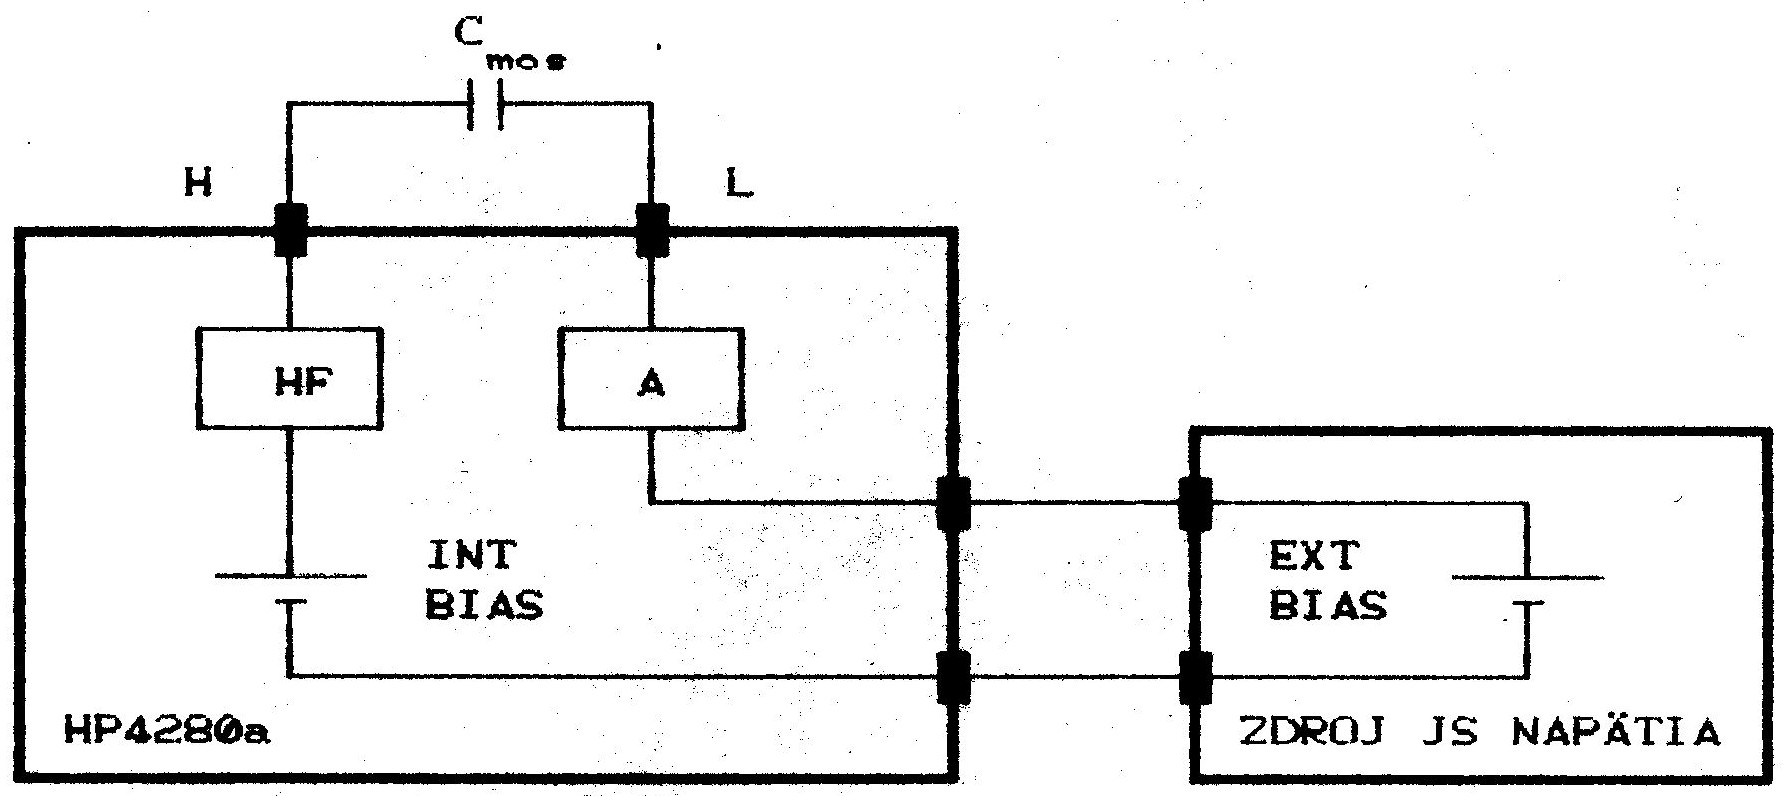
\includegraphics{Figures/fig-5-2.eps}
\captionsetup{justification=raggedright, singlelinecheck=false}
\caption[Zapojenie prístrojov pre metódu konštantnej šírky
  OPN]{Zapojenie prístrojov pre metódu konštantnej šírky OPN.}
\label{fig:5.2}
\end{figure}

Meranie zavislosti $V_{g}(t)$ potom prebieha v následovných
krokoch. Pomocou externého zdroja JS napätia privedieme štruktúru MOS
do nerovnovážneho stavu. Zo zmeny kapacity $\Delta{C}$, ktorú
odmeriame prístrojom HP4280a, vypočítame pomocou vzťahu \ref{eq:3.9}
požadovanú zmenu napätia hradla $\Delta{V_{g}}$ . Ak je jej veľkosť v
absolútnej hodnote väčšia ako $0.001 V$ zmeníme hodnotu napätia hradla
o $\Delta{V_{g}}$ , čím udržiavame konštantnú hodnotu nerovnovážnej
kapacity štruktúry MOS. Pri každej zmene napätia hradla odčítame čas,
kedy táto zmena nastala. Meranie závislosti $V_{g}(t)$ ukončíme, ak
uplynul čas merania (označme ho $T_{hold}$), ktorý zadáva operátor,
prípadne ak zmena hradlového napätia presiahla hraničné hodnoty
intervalu $(-2.0,+2.0) V$.  Experimentálne sa ukázalo, že programová
spätnoväzobná slučka zabezpečujúca konštantnú hodnotu kapacity pracuje
dostatočne rýchlo a presne. Počas prevádzaných experimentov bolo
kolísanie udržiavanej kapacity lepšie ako 1\%.

Meranie opakujeme pre rôzne hodnoty kapacity štruktúry MOS v
nerovnovážnom stave, aby sme mohli určiť generačnú dobu minoritných
nosičov náboja podľa vztahu \ref{eq:3.10}.

Parametrami riadiaceho programu je interval, v ktorom sa má pohybovat
hranica OPN $(W_{start}, W_{stop})$ s krokom $W_{step}$. Ďalším
parametrom je hodnota $T_{hold}$, ktorá udáva maximálnu dobu merania
jednej závislosti $V_{g}(t)$.

Riadiaci program vyžaduje pre svoju činnosť dátové súbory s nameranými
C-V závislosťami hlbokého ochudobnenia a kapacitami oxidovej vrstvy
testovaných štruktúr kremíkovej dosky. Pomocou týchto vopred
nameraných dát a zo zadanej vzdialenosti hranice OPN potom určuje
počiatočné hradlové napätie pre nastavenie externého zdroja JS
napätia.  Pre svoju činnosť potrebuje riadiaci program ešte jeden
dátovy súbor, obsahujúci koncentračné profily dotujúcich prímesí
meraných štruktúr MOS. Hodnoty koncentrácie sú potrebné pri
vyčíslovaní zmeny napätia hradla štruktúry MOS podľa vzťahu
\ref{eq:3.9}.

Po zmeraní závislosti $V_{g}(t)$ určíme lineárnou regresiou jej
smernicu.  Z uskutočnených experimentov sa ukazuje, že minimálna doba
merania zavislosti $V_{g}(t)$, kedy ešte možno očakávať akceptovateľné
výsledky je pre substráty s hodnotami $\tau_g$ rádove
$10^{3}\mu{s}$ približne $T_{hold}=10s$. Počas tejto doby
prichádzalo k zmene napätia hradla v rozsahu $50-500 mV$ v závislosti
od šírky OPN a v závislosti od prírastku minoritných nosičov z oblasti
mimo OPN. Zároveň bolo z grafického znázornenia závislosti
$\frac{dV_g}{dt}=f(w)$ vidieť vplyv prírastku minoritných nosičov náboja
z oblasti mimo OPN, čo sa prejavilo približne rovnakým sklonom
závislostí $\frac{dV_g}{dt}=f(w)$, ale rôznou absolútnou hodnotou.  Zo
zobrazenia závislostí $\frac{dV_g}{dt}=f(w)$ na celej kremíkovej doske
vyplýva, že akceptovateľné hodnoty $\tau_{g}$ možno počítať jedine z
derivácie funkcie $\frac{dV_g}{dt}=f(w)$ podľa w (vzťah \ref{eq:3.10}
príp. \ref{eq:3.7}) a v žiadnom prípade nie z jej fukčných hodnôt
(vzťah \ref{eq:3.5}). Do výstupného dátového súboru sme ukladali
funkčné závislosti $\frac{dV_g}{dt}=f(w)$.

Z princípu metódy vyplýva minimálna vzdialenosť od povrchu polovodiča,
v ktorej je možno určovať $\tau_{g}$. Touto hranicou je šírka OPN
zodpovedajúca počiatku slabej inverzie v polovodiči.

\section{Časové diagramy použitých metód.}\label{sec:5.4}

Aby sme mohli odhadnúť dobu merania pre jednotlivé metódy, znázorníme
graficky časové závislosti hradlového napätia štruktúry MOS. Okrem
rovnovážnej HF C-V metódy, kde je celý priebeh merania riadený
procesorom prístroja HP4280a a jeho časový diagram je prevzatý z
manuálu \cite{5.7}, boli časové diagramy určené na základe
experimentálne nameraných hodnôt. Tieto časové hodnoty sú závislé od
druhu riadiaceho počítača a od optimalizácie riadiacich programov. V
našom experimente sme použili osobný počítač PC AT, pracujúci na
frekvencii 10 MHz s koprocesorom 80287 (6 MHz) a pevným diskom s dobou
prístupu 28 ms. Riadiace programy boli kompilované bez optimalizácie
na rýchlosť s použitím emulačnej knižnice podprogramov pre matematické
operácie s plávajúcou čiarkou.

V spojení s časovými diagramami uvedieme aj rozsahy napätí použitých
prístrojov.

\par\emph{POZNÁMKA.} V prípade, ak je pri maximálnej hodnote časového
údaju uvedený údaj 'neohraničené', znamená to, že jeho maximálna
veľkosť závisí od dátového typu zodpovedajúcej premennej riadiaceho
programu, prípadne od rozsahu prístroja.


\newpage
\subsection{Rovnovážna HF C-V závislosť.}\label{sec:5.4.1}

\begin{figure}[h!]\centering
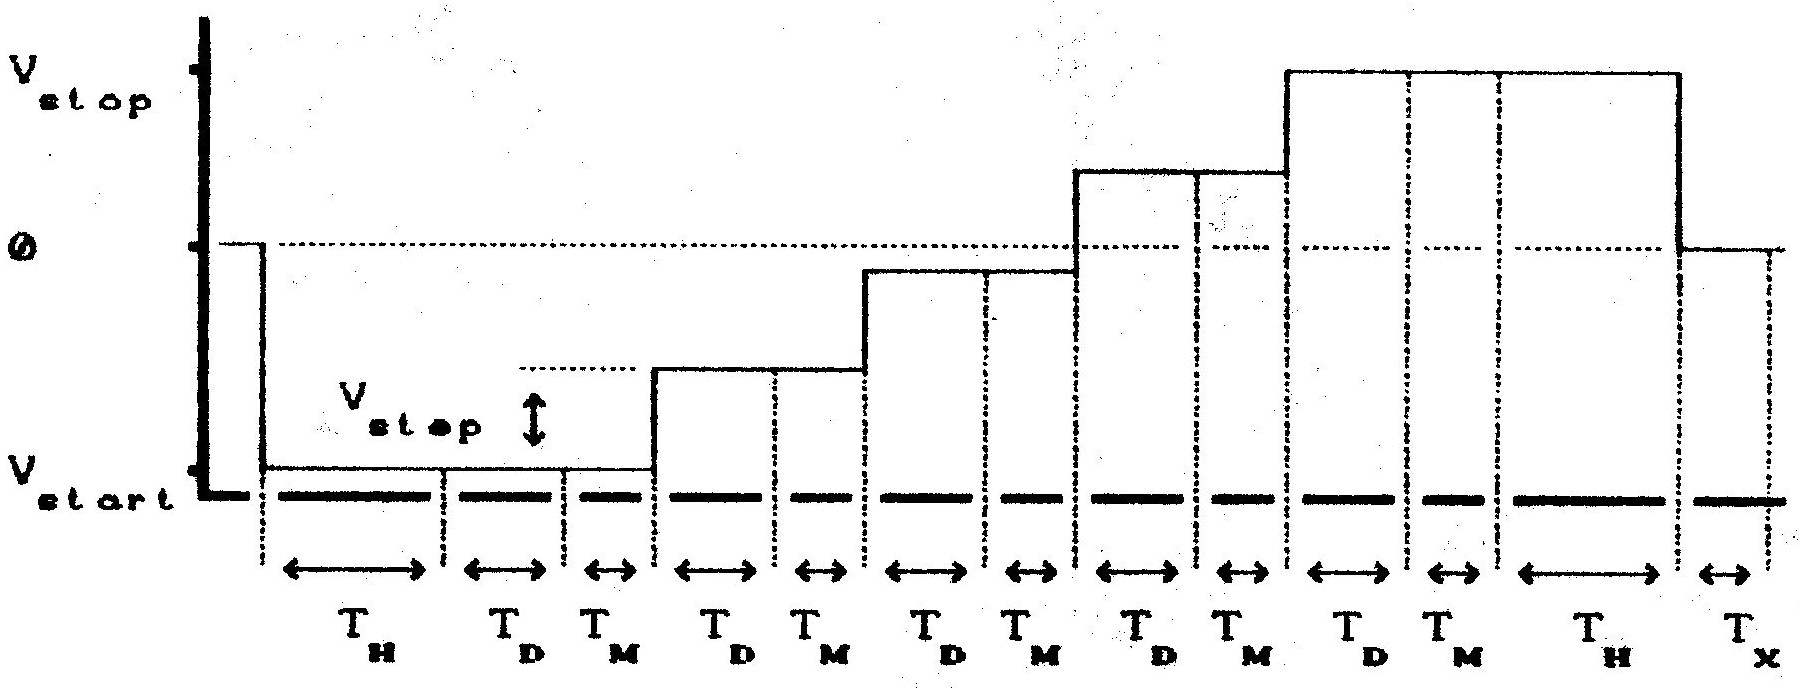
\includegraphics{Figures/fig-5-3.eps}
\captionsetup{justification=raggedright, singlelinecheck=false}
\caption[Časový diagram rovnovážnej HF C-V metódy]{Časový diagram
  rovnovážnej HF C-V metódy.}
\label{fig:5.3}
\end{figure}

\begin{table}[h!]\centering
\begin{tabular}{ l p{0.5\linewidth} l l }
\hline
parameter   & popis parametra & min. & max.hodnota \\
\hline
$T_H$       & čas ustálenia \dotfill & $3 ms$ &  $650 s$\\
$T_D$       & čas pozdržania merania \dotfill & $3 ms$ & $650 s$ \\
$T_M$       & čas merania \dotfill & $40 ms$ \\
$T_X$       & binárny prenos dát,\\
            & predspracovanie dát,\\
            & uloženie dát do súboru,\\
            & posuv stolíka na ďalšiu štruktúru \dotfill & $\sim 7 s$ \\
$V_{start}$ & \dotfill & $-100.0 V$ & $+100.0 V$ \\
$V_{stop}$  & \dotfill & $-100.0 V$ & $+100.0 V$ \\
$V_{step}$  & \dotfill & $\pm 0.001 V$ & $\pm 200.0 V$ \\
\hline
\end{tabular}
\caption[Časový diagram rovnovážnej HF C-V metódy]{Časový diagram
  rovnovážnej HF C-V metódy.}
\label{tab:5.1}
\end{table}

\newpage
\subsection{Nerovnovážna HF C-V závislosť.}\label{sec:5.4.2}

\begin{figure}[h!]\centering
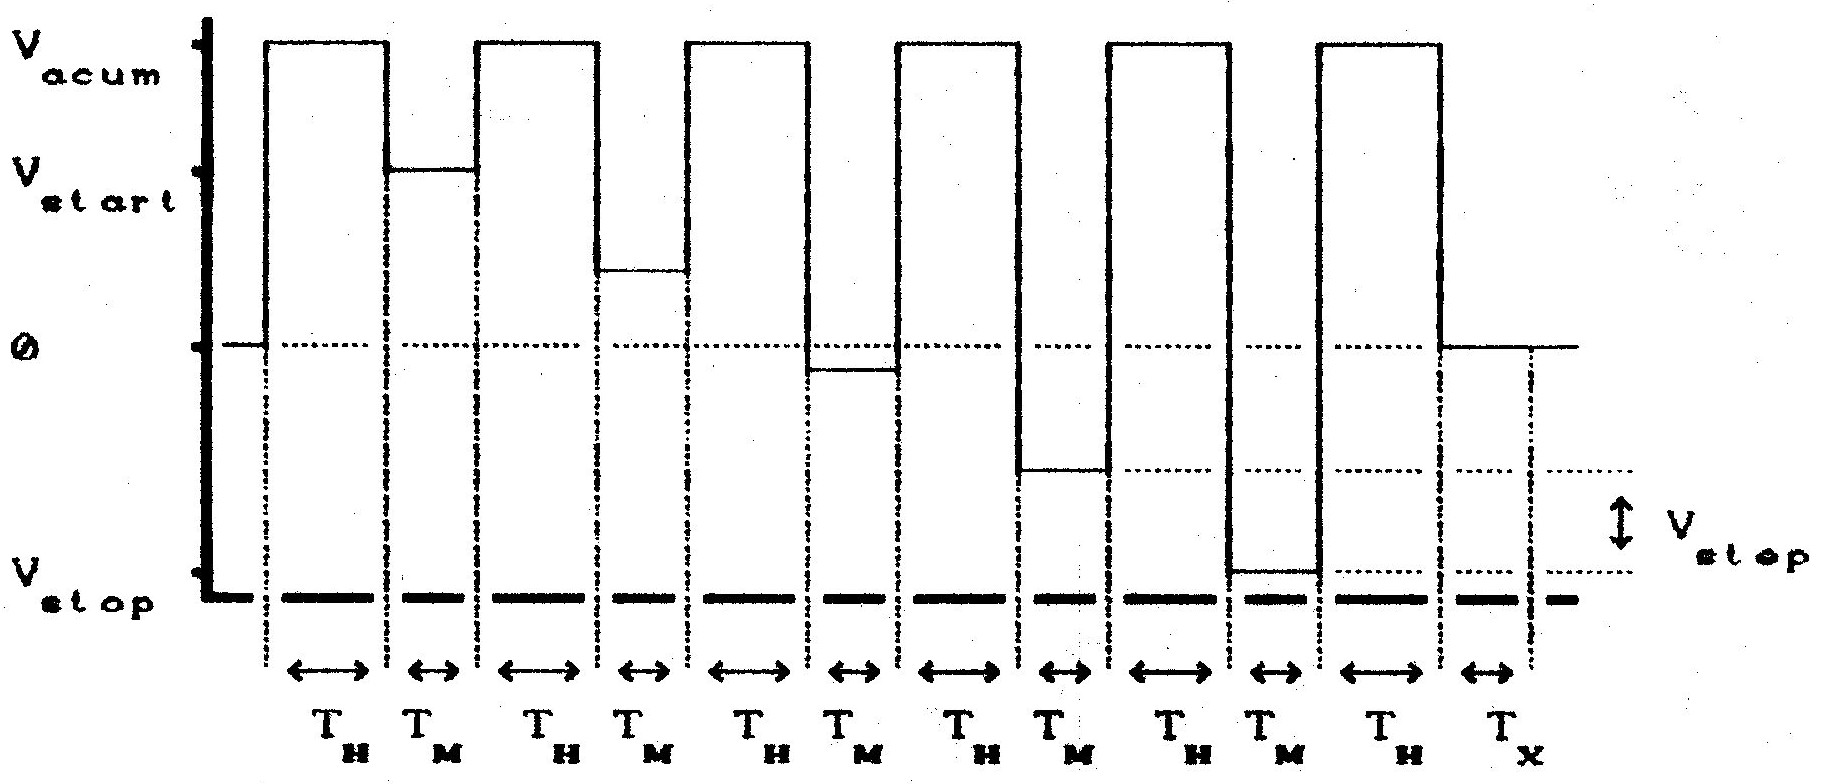
\includegraphics{Figures/fig-5-4.eps}
\captionsetup{justification=raggedright, singlelinecheck=false}
\caption[Časový diagram nerovnovážnej HF C-V metódy]{Časový diagram
  nerovnovážnej HF C-V metódy.}
\label{fig:5.4}
\end{figure}

\begin{table}[h!]\centering
\begin{tabular}{ l p{0.5\linewidth} l l }
\hline
parameter   & popis parametra & min. & max.hodnota \\
\hline
$T_H$  & čas relaxácie minoritných nosičov náboja \dotfill & $0 s$ &  neohraničené \\
$T_M$  & čas merania a prenos dát \dotfill & $330 ms$ \\
$T_X$  & predspracovanie dát, \\
       & uloženie dát do súboru, \\
       & posuv stolíka na ďalšiu štruktúru \dotfill & $\sim 4 s$ \\
$V_{start}$ & \dotfill & $-100.0$ & $+100.0 V$ \\
$V_{stop}$ & \dotfill & $-100.0$ & $+100.0 V$ \\
$V_{step}$ & \dotfill & $\pm 0.001$ & $\pm 200.0 V$ \\
$V_{acum}$ & \dotfill & $-100.0$ & $+100.0 V$ \\
\hline
\end{tabular}
\caption[Časový diagram nerovnovážnej HF C-V metódy]{Časový diagram
  nerovnovážnej HF C-V metódy.}
\label{tab:5.2}
\end{table}

\newpage
\subsection{Kvázistatická C-V závislosť.}\label{sec:5.4.3}

\begin{figure}[h!]\centering
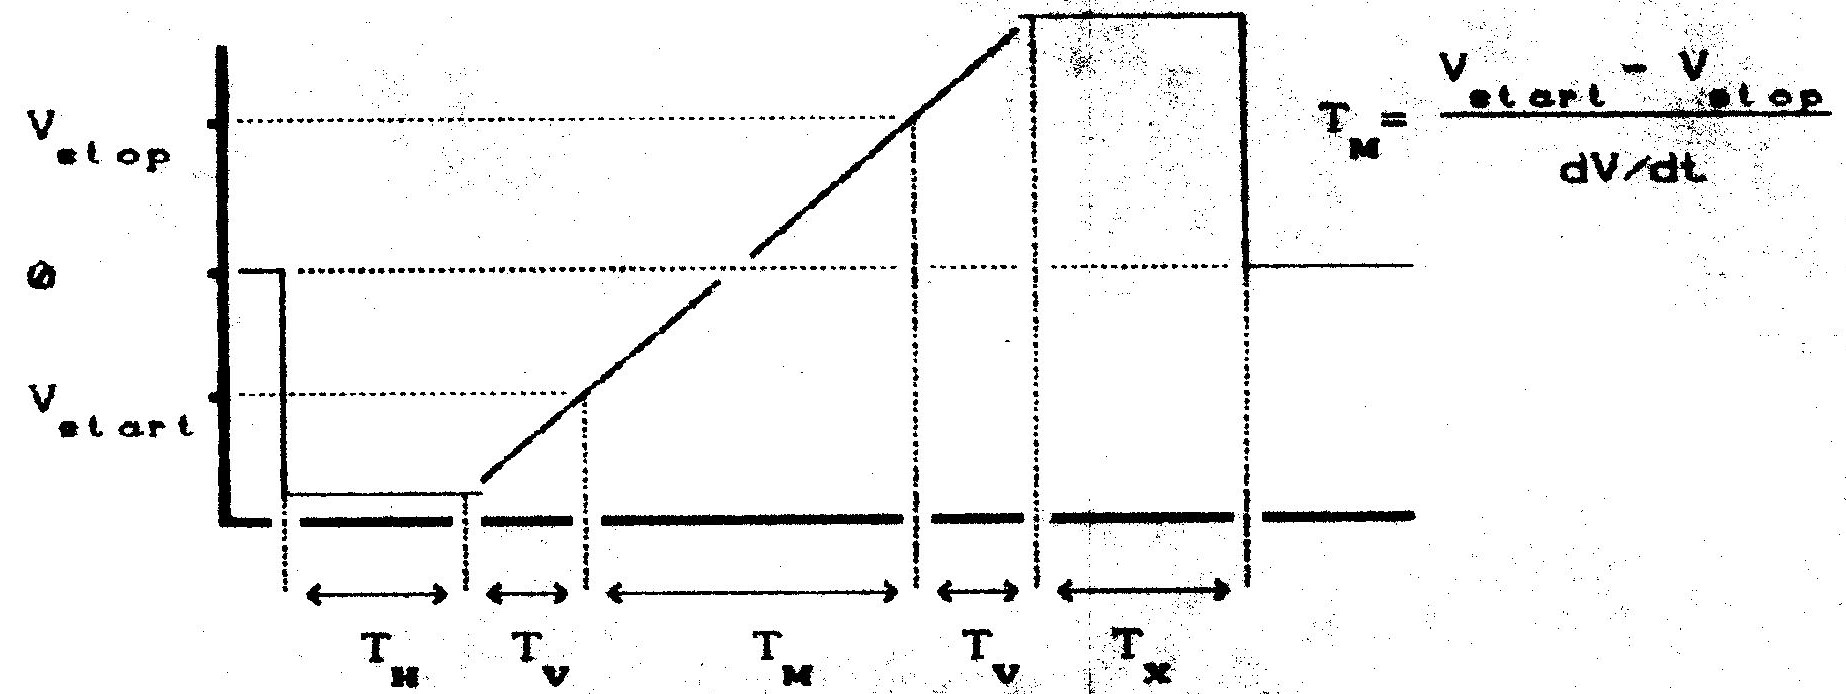
\includegraphics{Figures/fig-5-5.eps}
\captionsetup{justification=raggedright, singlelinecheck=false}
\caption[Časový diagram kvázistatickej C-V metódy]{Časový diagram
  kvázistatickej C-V metódy.}
\label{fig:5.5}
\end{figure}

\begin{table}[h!]\centering
\begin{tabular}{ l p{0.5\linewidth} l l }
\hline
parameter   & popis parametra & min. & max.hodnota \\
\hline
$T_H$  & čas ustálenia \dotfill & $0 s$ & neohraničené \\
$T_V$  & čas merania napätia hradla a času \dotfill & $5 s$ \\
$T_M$  & čas merania prúdu a času \dotfill & neohraničené\\
$T_X$  & predspracovanie dát, \\
       & uloženie dát do súboru, \\
       & posuv stolíka na ďalšiu štruktúru \dotfill & $\sim 15 s$ \\
$V_{start}$ & \dotfill & $-20.0$ & $+20.0 V$ \\
$V_{stop}$ & \dotfill & $-20.0$ & $+20.0 V$ \\
$dV/dt$ & \dotfill & $\pm 0.1mV/s$ & $\pm 10.0V/s$ \\
\hline
\end{tabular}
\caption[Časový diagram kvázistatickej C-V metódy]{Časový diagram
  kvázistatickej C-V metódy.}
\label{tab:5.3}
\end{table}

\newpage
\subsection{Metóda konštantnej šírky OPN.}\label{sec:5.4.4}

\begin{figure}[h!]\centering
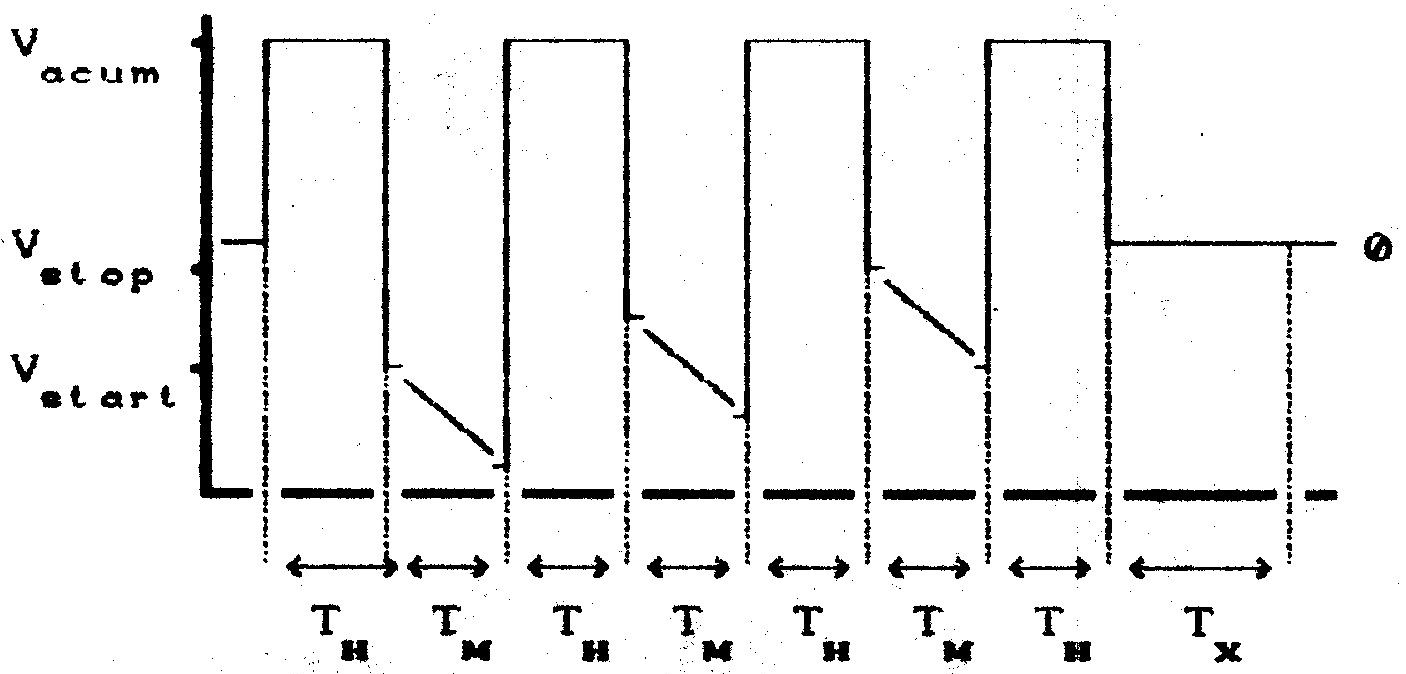
\includegraphics{Figures/fig-5-6.eps}
\captionsetup{justification=raggedright, singlelinecheck=false}
\caption[Časový diagram metódy konštantnej šírky OPN]{Časový diagram
  metódy konštantnej šírky OPN}.
\label{fig:5.6}
\end{figure}

\begin{table}[h!]\centering
\begin{tabular}{ l p{0.5\linewidth} l l }
\hline
parameter   & popis parametra & min. & max.hodnota \\
\hline
$T_H$ & čas relaxácie minoritných nosičov náboja \dotfill & $0 s$ & neohraničené \\
$T_M$ & čas merania, výpočet $dV/dt$ \dotfill & $10 s$ & neohraničené \\
$T_X$ & uloženie dát do súboru, \\
      & posuv stolíka na ďalšiu štruktúru \dotfill & $\sim 2 s$ \\
$V_{start}$ & \dotfill & $-40.0$ & $+40.0 V$ \\
$V_{stop}$  & \dotfill & $-40.0$ & $+40.0 V$ \\
$V_{acum}$  & \dotfill & $-40.0$ & $+40.0 V$ \\
\hline
\end{tabular}
\caption[Časový diagram metódy konštantnej šírky OPN]{Časový diagram
  metódy konštantnej šírky OPN.}
\label{tab:5.4}
\end{table}


\begin{thebibliography}{}
\bibitem[5.1]{5.1} Mariassy P. : Riadiaca jednotka prístroja typu
  talker/listener na spojenie so zbernicou IMS. Diplomová práca. EF
  SVŠT Bratislava 1988.
\bibitem[5.2]{5.2} National Instruments, IEEE-488 Instrumentation
  Interface. User guide.
\bibitem[5.3]{5.3} Keithley model 642, Instruction manual.
\bibitem[5.4]{5.4} Marčuk G.I.: Metódy numerické matematiky. Academia
  Praha 1987.
\bibitem[5.5]{5.5} Cox M.G. : J. Inst. Maths. Aplics. , 10 (1972)
  s.134.
\bibitem[5.6]{5.6} De Boor C. : J. Approx. Theory, 6 (1972) s.50.
\bibitem[5.7]{5.7} Hewlett-Packard, Operational and service manual,
  Model HP4280a.
\end{thebibliography}
 
% Chapter 6

\chapter{Spracovanie dát a zobrazenie získanych parametrov štruktúr MOS.} % Main chapter title

\label{Chapter6} % For referencing the chapter elsewhere, use \ref{Chapter1} 

\lhead{Chapter 6. \emph{Spracovanie dát a zobrazenie získaných parametrov štruktúr MOS}}

V tejto kapitole uvedieme stručne postup spracovania dát, nameraných
pomocou programov zberu dát a zameriame sa na plošné zobrazenie
získaných parametrov štruktúr MOS. Metodika výpočtu parametrov
štruktúr MOS bola popísaná v kapitolách 3 a 4, na ktoré sa budeme
odvolávať.

Väčšina parametrov je určovaná z nameraných dát pomocou samostatných
programov a ukladaná do dátových súborov, ktorých štruktúra bola
popísaná v časti 5. Plošné rozloženie vypočítaných parametrov štruktúr
MOS možno potom zobraziť na displeji počítača. Pri zobrazovaní na
displeji je k dispozícii 16 farieb, avšak pri zobrazení obrázkov na
tlačiarni bolo kvôli lepšej rozlišiteľnosti použitých len 6
farieb. Orientácia kremíkovej dosky na obrázkoch je smerom 'fazetou
hore', pričom jeden štvorček zobrazenej plochy predstavuje hodnotu
parametra štruktúry MOS. Farba štvorčeka závisí od intervalu, do
ktorého daná hodnota spadá. Škála intervalov je zobrazená v pravej
časti obrázku, pričom číslo uvedené pri jednotlivých farbách
predstavuje dolnú hranicu intervalu. Pretože sa farby v škále
intervalov viackrát opakujú, bolo potrebné označiť, v ktorých
intervaloch sa zobrazované hodnoty nachádzajú. To je označené veľkým
písmenom 'X' medzi dolnou hranicou intervalu a prislúchajúcou
farbou. Možno ešte poznamenať, že náhodne odlišné výsledky v
niektorých bodoch kremíkovej dosky spôsobia, že sa v škále intervalov
objaví vyznačený interval, ktorý zjavne nesúvisí s ostatnými
hodnotami, čo možno pripísat nefunkčnej štruktúre MOS. Treba ešte
upozorniť, že orientácia škály sa môže pri zobrazení rôznych
parametrov meniť.

\section{Určenie koncentračného profilu dotujúcich prímesí, dávky implantácie a napätia vyrovnaných pásov.}\label{sec:6.1}

Určenie koncentračného profilu dotujúcich prímesí vykonáva samostatný
program, ktorý ako vstupné dáta vyžaduje súbory (a) nameraných HF C-V
závislostí a (b) nameraných kapacít oxidovej vrstvy štruktúry
MOS. Výstupom programu je dátový súbor obsahujúci hĺbkové priebehy
koncentračných profilov skúmaných štruktúr MOS, ktoré sú počítané
podľa vzťahov uvedených v časti \ref{sec:4.1}. Ak boli v procese zberu
dát zmerané aj kvázistatické C-V závislosti, program vykoná korekciu
koncentračného profilu na hustotu pascí rozhrania
$Si-SiO_2$. Povrchový potenciál určujeme podľa vzťahov \ref{eq:4.3} a
\ref{eq:4.4} a používame ho pre korekciu aproximácie hlbokého
ochudobnenia pri povrchu polovodiča a pre výpočet hĺbky (šírky
OPN). Vedľajším produktom je dátovy súbor obsahujúci napätia
vyrovnaných pásov $V_{fb}$, ktoré sa určujú v bode C-V závislosti, pre
ktoré povrchový potenciál $\varphi_s$ mení znamienko. Obrázok
\ref{fig:6.1} predstavuje plošné rozloženie koncentrácie v rôznych
hĺbkach polovodiča a na obrázku \ref{fig:6.2} je znázornené rozloženie
$V_{fb}$. Koncentračný profil prímesí bol vytvorený implantáciou
$P^{31}$ s dávkou $4.0\times 10^{15} m^{-2}$ pri energii $120
keV$. Aktivácia prebiehala počas 40 minút pri teplote $1050 \degree C$
v atmosfére $N_2$. Stredná hodnota $N(x)$ je spolu s ďalšími priebehmi
pre rôzne implantačné dávky zobrazená na obrázku \ref{fig:7.3}.

Pre známe priebehy koncentračných profilov môžeme vypočítať dávku
implantácie podľa vzťahu

\begin{equation}\label{eq:6.1}
D = \int_{0}^{x_{1}}(N(x) - N_{b}) dx
\end{equation}

kde predpokládame, že poznáme priebeh N(x) do vzdialenosti $x_{1}$ ,
pre ktorú platí

\begin{equation}\label{eq:6.2}
N(x) = N_{b} \qquad {x \ge x_{1}}
\end{equation}

Dávka $D$ vypočítaná týmto spôsobom predstavuje časť implantovaných
iónov, ktoré sa dostali v priebehu implantácie do polovodiča a boli
aktivované v poimplantačnom tepelnom spracovaní. Na obrázku
\ref{fig:6.3} je znázornené plošné rozloženie dávky na testovanej
kremíkovej doske určenej zo závislosti $N(x)$ zobrazených na obrázku
\ref{fig:6.1}.

\begin{figure}[h!]\centering
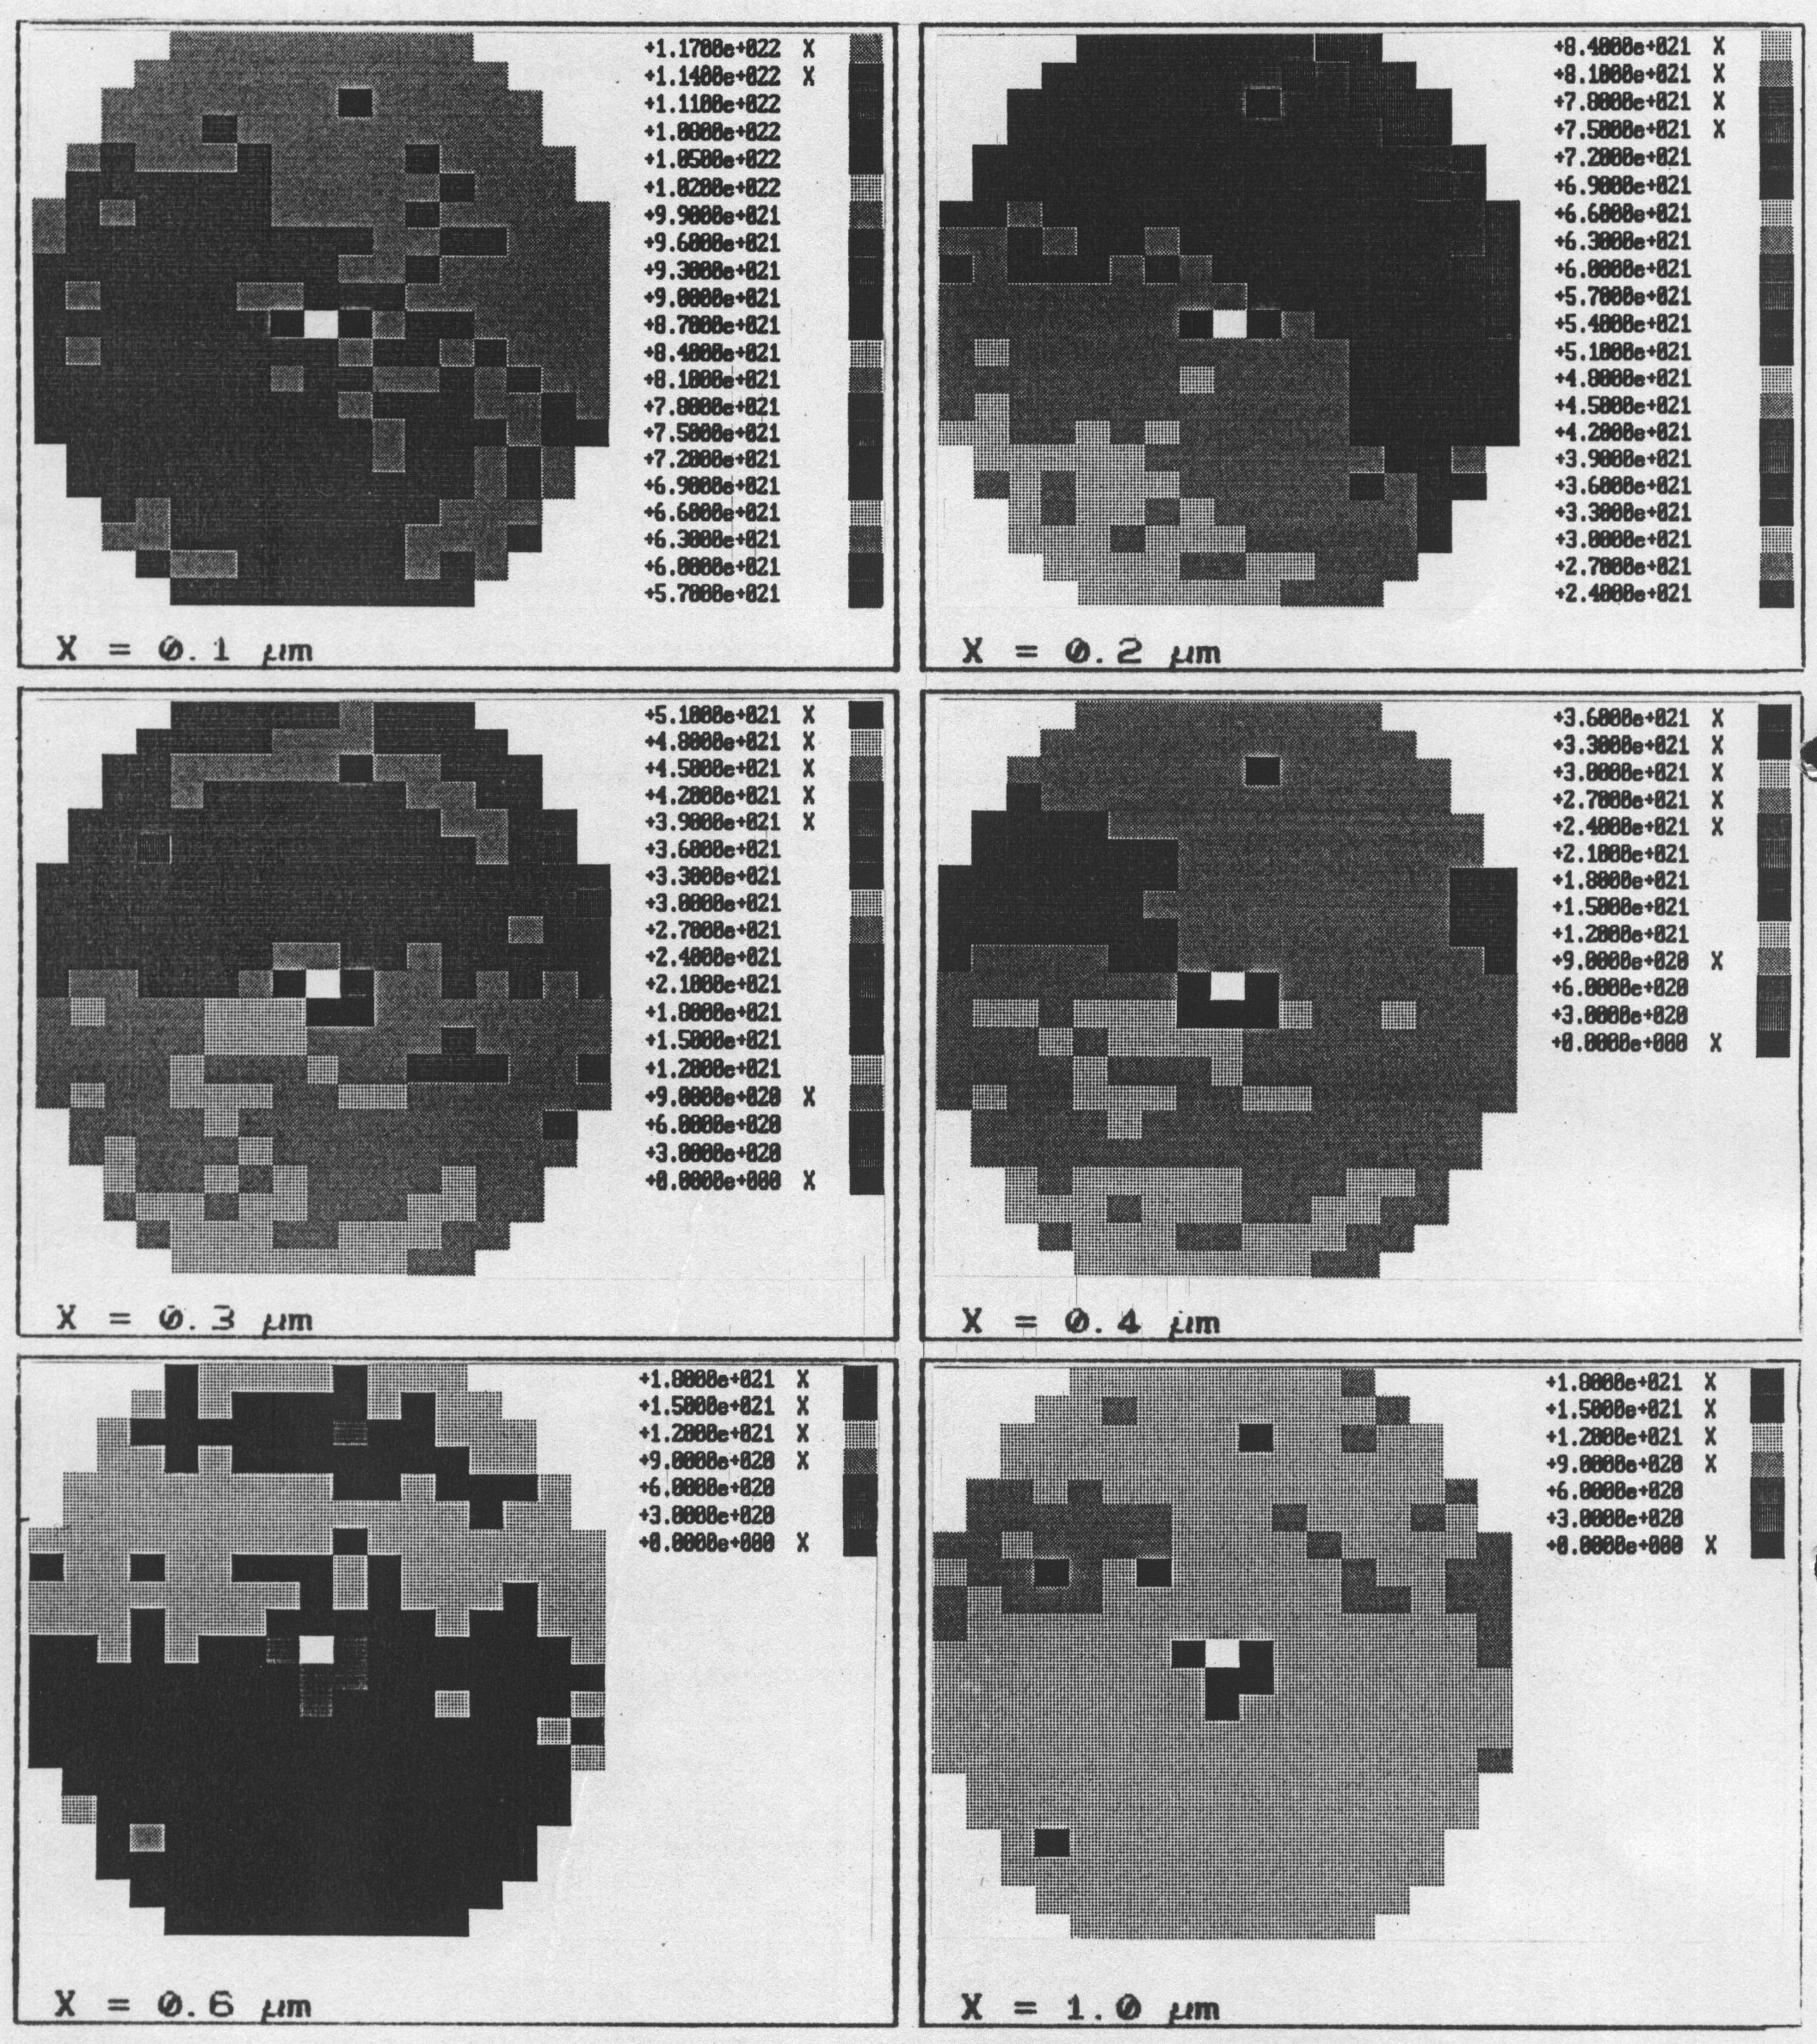
\includegraphics{Figures/fig-6-1.eps}
\captionsetup{justification=raggedright, singlelinecheck=false}
\caption[Rozloženie dotujúcich prímesí $N(x)$ v rôznej hĺbke
  $x$]{Rozloženie dotujúcich prímesí $N(x)$ v rôznej hĺbke $x$ pod
  povrchom polovodiča pre dávku implantácie $4.0 \times 10^{15}
  m^{-2}$.}
\label{fig:6.1}
\end{figure}

\begin{figure}[h!]\centering
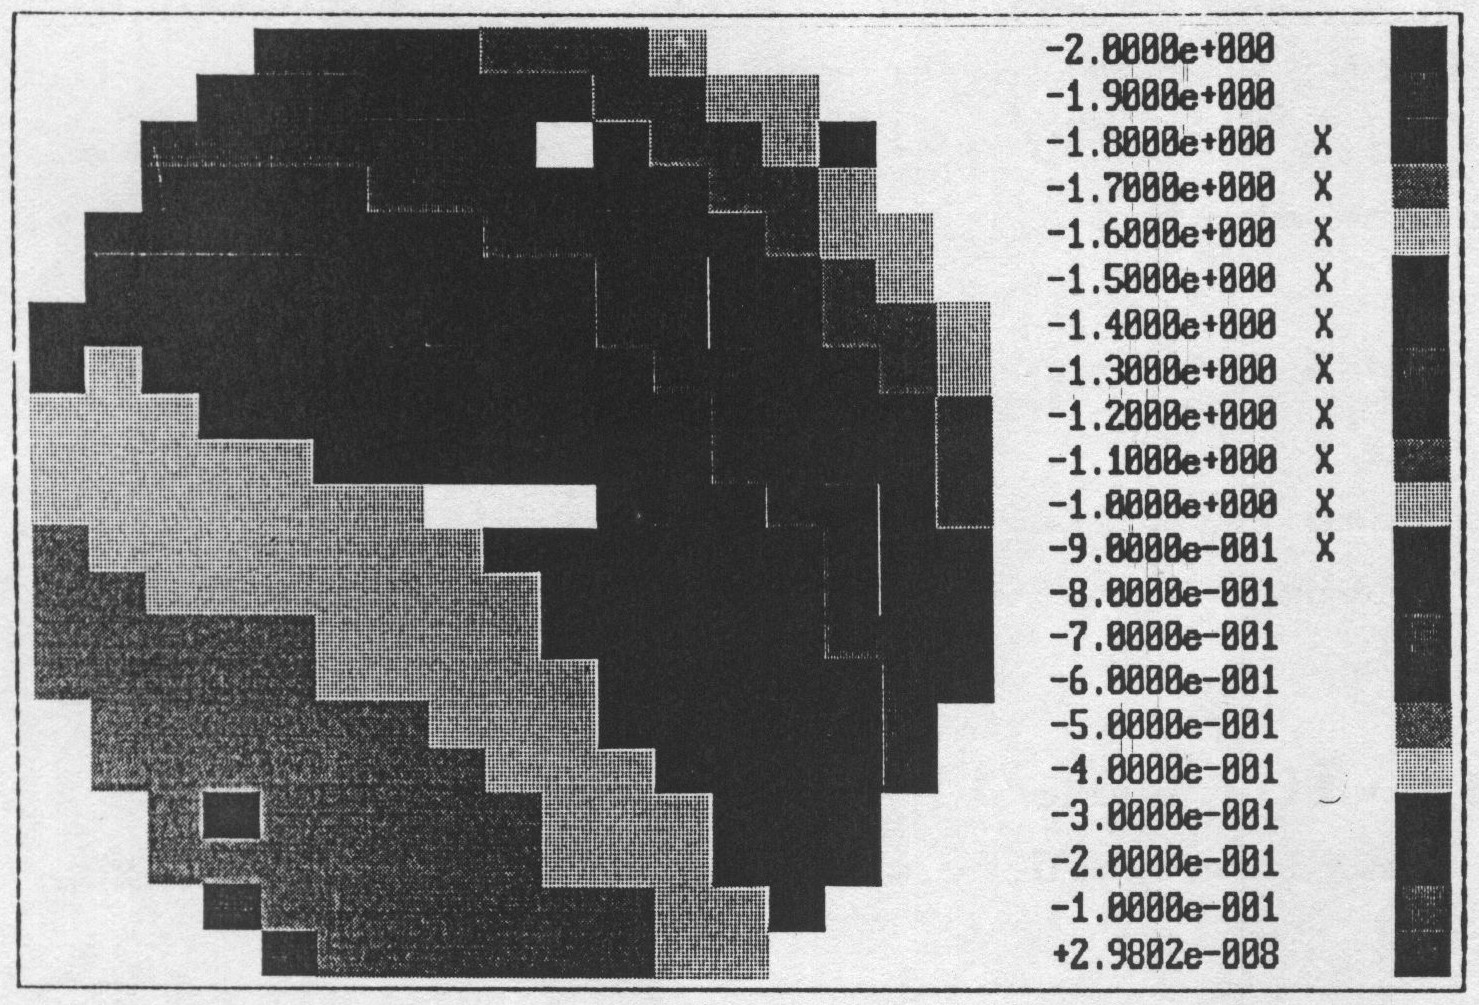
\includegraphics{Figures/fig-6-2.eps}
\captionsetup{justification=raggedright, singlelinecheck=false}
\caption[Plošné rozloženie $V_{fb}$]{Plošné rozloženie $V_{fb}$ určené
  pri výpočte $N(x)$ z obrázka \ref{fig:6.1}.}
\label{fig:6.2}
\end{figure}

\begin{figure}[h!]\centering
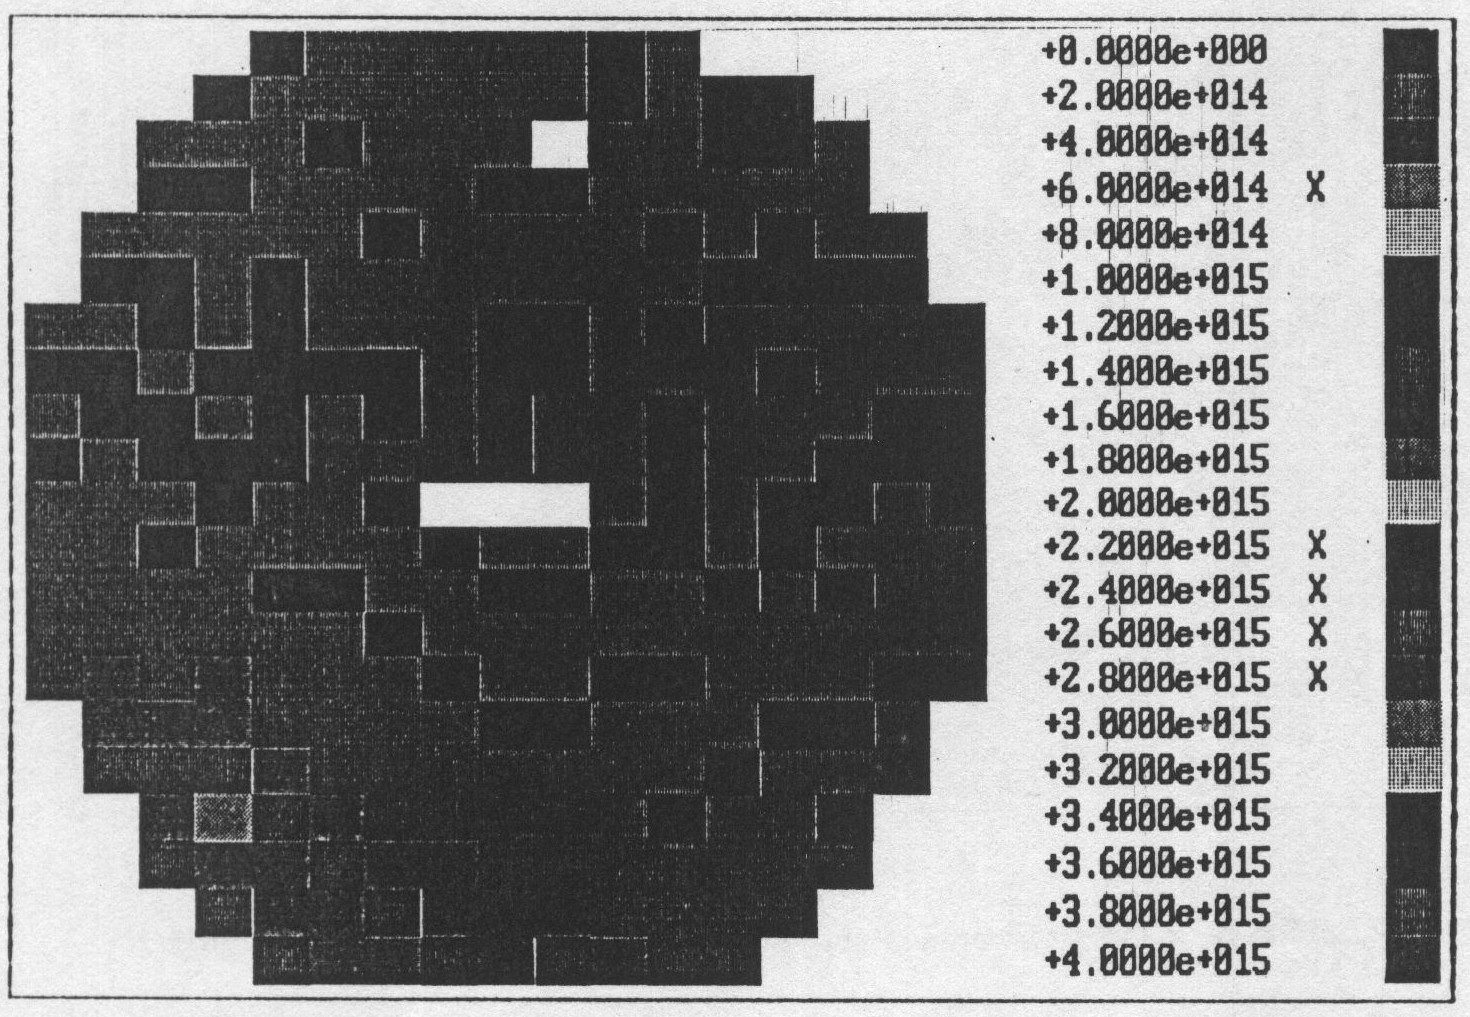
\includegraphics{Figures/fig-6-3.eps}
\captionsetup{justification=raggedright, singlelinecheck=false}
\caption[Plošné rozloženie nameranej dávky implantácie]{Plošné
  rozloženie nameranej dávky implantácie pre profil N(x) z obrázka
  \ref{fig:6.1}.}
\label{fig:6.3}
\end{figure}


\section{Určenie hrúbky oxidovej vrstvy.}\label{sec:6.2}

Ak poznáme kapacitu oxidovej vrstvy štruktúry MOS a jej plochu, potom
môžeme vypočítať jej hrúbku podľa vzťahu

\begin{equation}\label{eq:6.3}
h_{ox} = A \frac{\epsilon}{C_{ox}}
\end{equation}

kde sme použili hodnotu relatívnej permitivity $SiO_{2}$
$\epsilon_{r}=3.9$. Plošné rozloženie hrúbky oxidovej vrstvy je potom
zobrazené na obrázku \ref{fig:6.4}.

\begin{figure}[h!]\centering
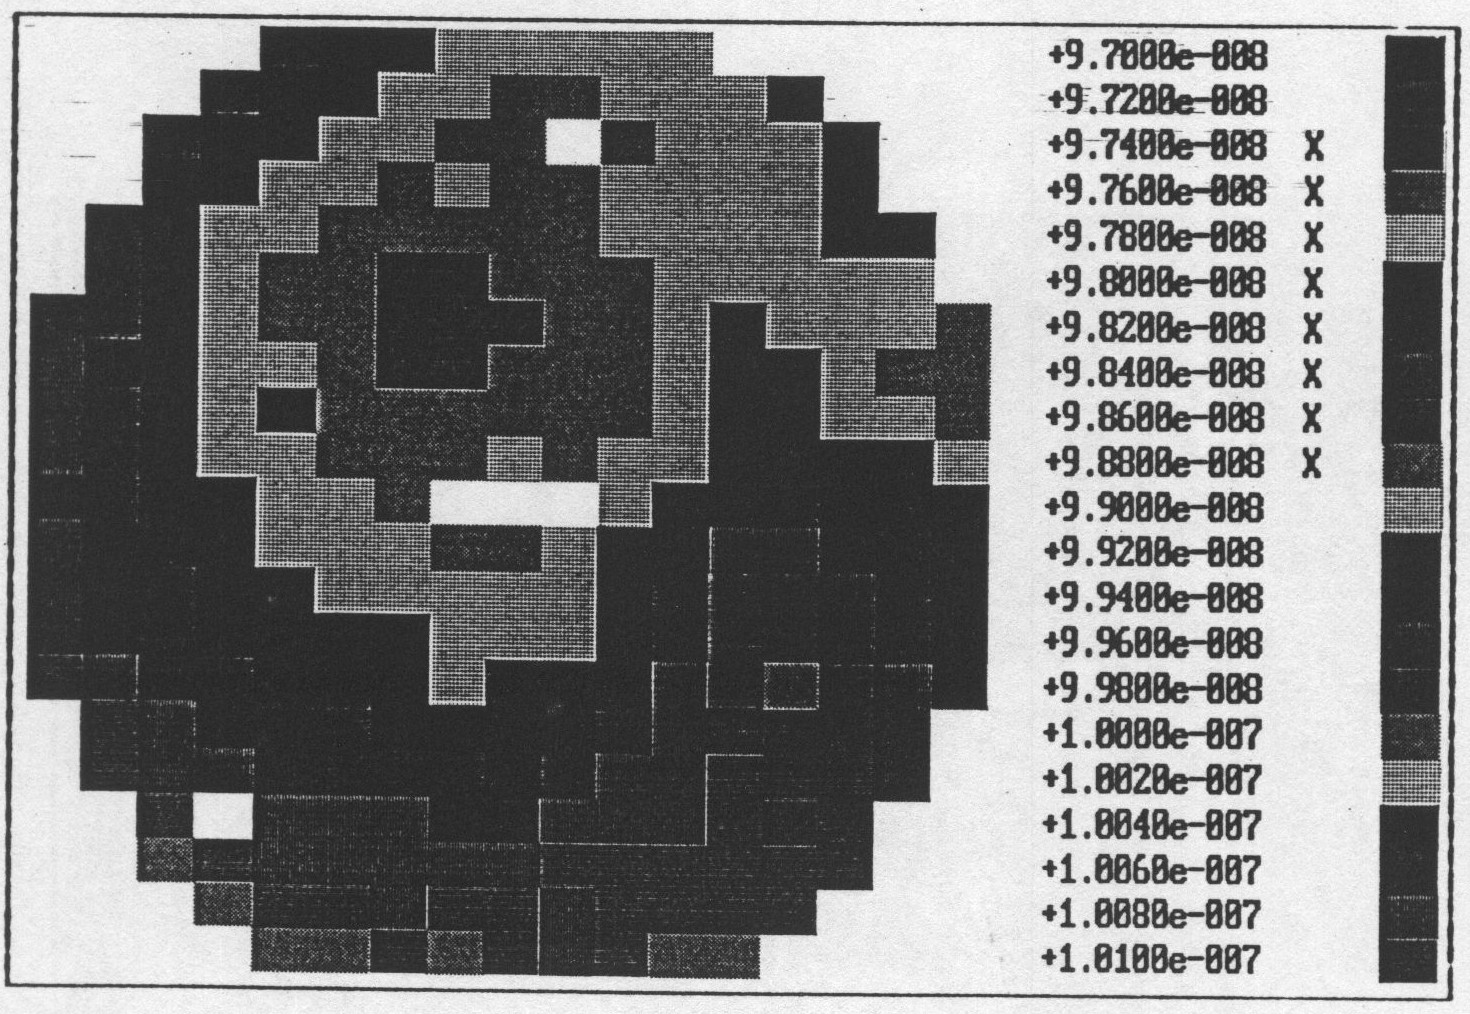
\includegraphics{Figures/fig-6-4.eps}
\captionsetup{justification=raggedright, singlelinecheck=false}
\caption[Plošné rozloženie hrúbky hradlového oxidu $h_{ox}$]{Plošné
  rozloženie hrúbky hradlového oxidu $h_{ox}$.}
\label{fig:6.4}
\end{figure}


\section{Určenie hustoty pascí rozhrania $Si-SiO_{2}$.}\label{sec:6.3}

Pre výpočet hustoty pascí rozhrania použijeme porovnanie HF a
kvázistatickej C-V závislosti, kde použijeme postup popísany v časti
\ref{sec:4.2.1}. Možno poznamenať, že pre určenie polohy Fermiho
hladiny na povrchu polovodiča použijeme hodnoty povrchového potenciálu
$\varphi_{s}(V_{g})$, získané integráciou kvázistatickej C-V
závislosti a hodnotu integračnej konštanty $\varphi_{s0}$ určíme
postupom popísaným v dodatku \ref{app:AppendixG}.

Celý postup výpočtu $D_{it}$ je realizovaný dvoma programami. Prvý program na základe zmeraných kvázistatických C-V závislostí a známych hĺbkových priebehov $N(x)$ vypočíta závislosti $\varphi_{s}(V_{g})$, ktoré uloží do dátového súboru.  Druhý program pre svoju činnosť vyžaduje dátove súbory

\begin{itemize}
\item HF C-V závislosti $C_{mos}^{HF}(V_{g})$
\item kvázistatické C-V závislosti $C_{mos}^{LF}(V_{g})$
\item závislosť povrchového potenciálu od napätia hradla $\varphi_{s}(V_{g})$.
\end{itemize}

Vypočítané hodnoty $D_{it}$ ako závislosť polohy Fermiho hladiny v
zakázanom pásme polovodiča uloží do dátoveho súboru. Na obrázku
\ref{fig:6.5} je zobrazené plošné rozloženie $D_{it}$ v strede
zakázaného pásma.

\begin{figure}[h!]\centering
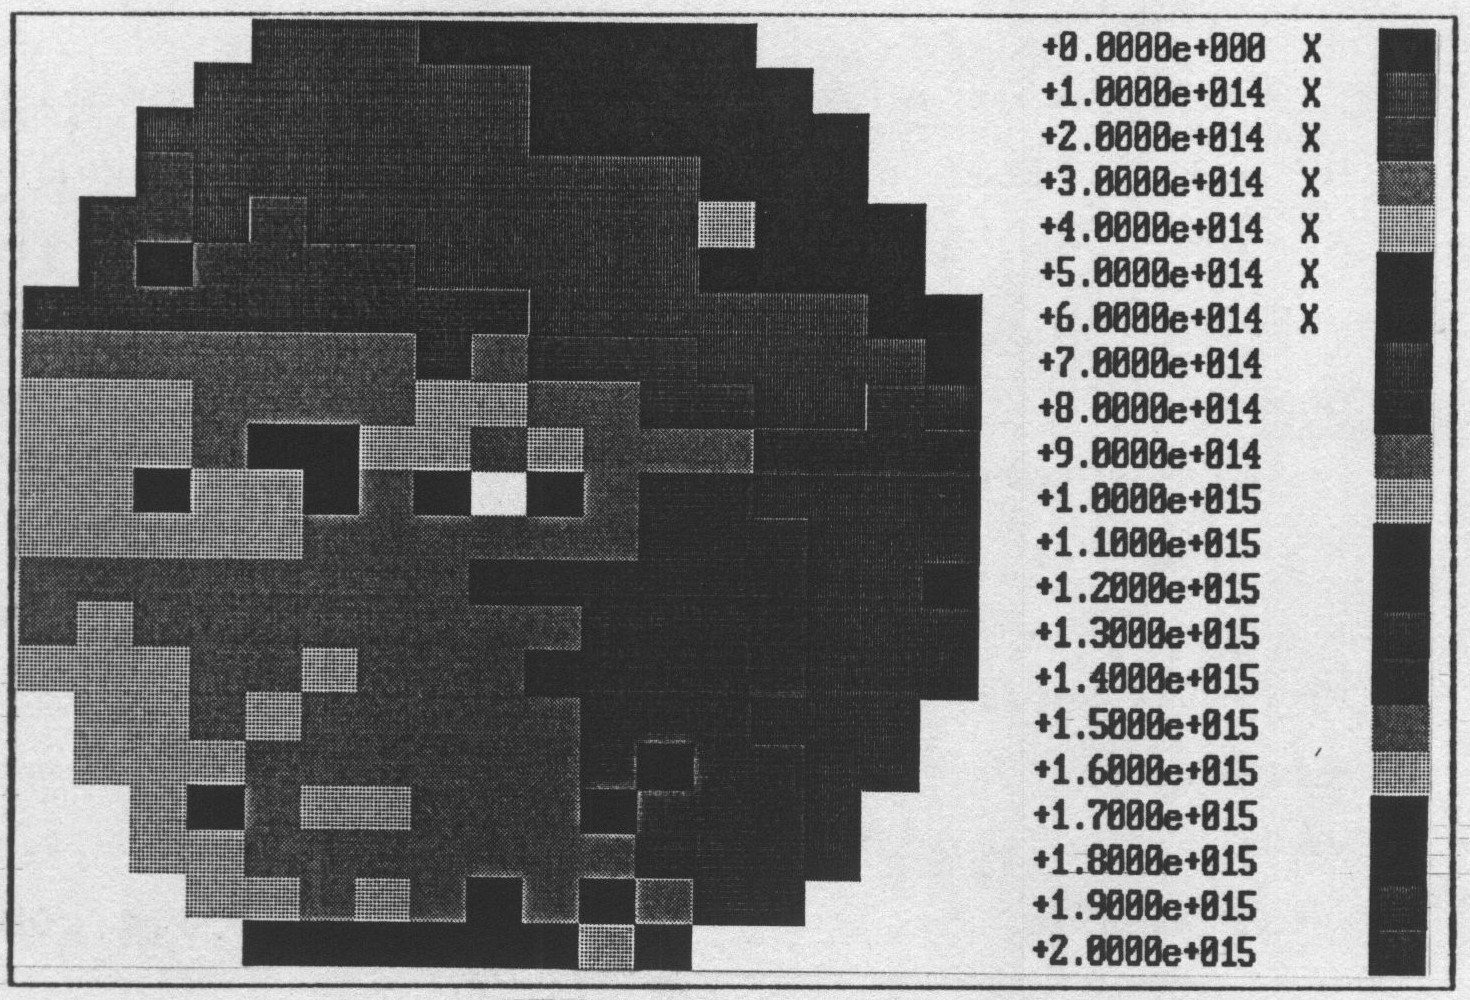
\includegraphics{Figures/fig-6-5.eps}
\captionsetup{justification=raggedright, singlelinecheck=false}
\caption[Plošné rozloženie hustoty pascí rozhrania $Si-SiO_{2}$ v
  strede zakázaného pásma]{Plošné rozloženie hustoty pascí rozhrania
  $Si-SiO_{2}$ v strede zakázaného pásma.}
\label{fig:6.5}
\end{figure}


\section{Určenie generačného času života minoritných nosičov náboja.}\label{sec:6.4}

V procese zberu dát metódou konštantnej šírky OPN bol vytvorený dátovy
súbor obsahujúci smernice závislostí $V_{g}(t)$ pre rôzne šírky OPN
testovaných štruktúr MOS kremíkovej dosky. Pre určenie generačného
času života minoritných nosičov náboja podľa vzťahu \ref{eq:3.10} je
dôležité ako vypočítame deriváciu závislosti smerníc $V_{g}(t)$ podľa
vzdialenosti hranice OPN od povrchu polovodiča. Použitie číslicových
filtrov v tomto prípade nie je vhodné, pretože máme k dispozícii málo
bodov závislosti $dV_{g}/dt = f(w)$. V tomto prípade možno pužiť
aproximáciu lokálnymi polynómami. Teoretický základ aj zdrojový text
procedúry v jazyku Algol je uvedený napríklad v \cite{6.1}. Na obrázku
\ref{fig:6.6} je zobrazené plošné rozloženie generačnej doby
minoritných nosičov náboja, ktorá predstavuje jej strednú hodnotu v
oblasti od $0.9 \mu m$ do $1.3 \mu m$.

\begin{figure}[h!]\centering
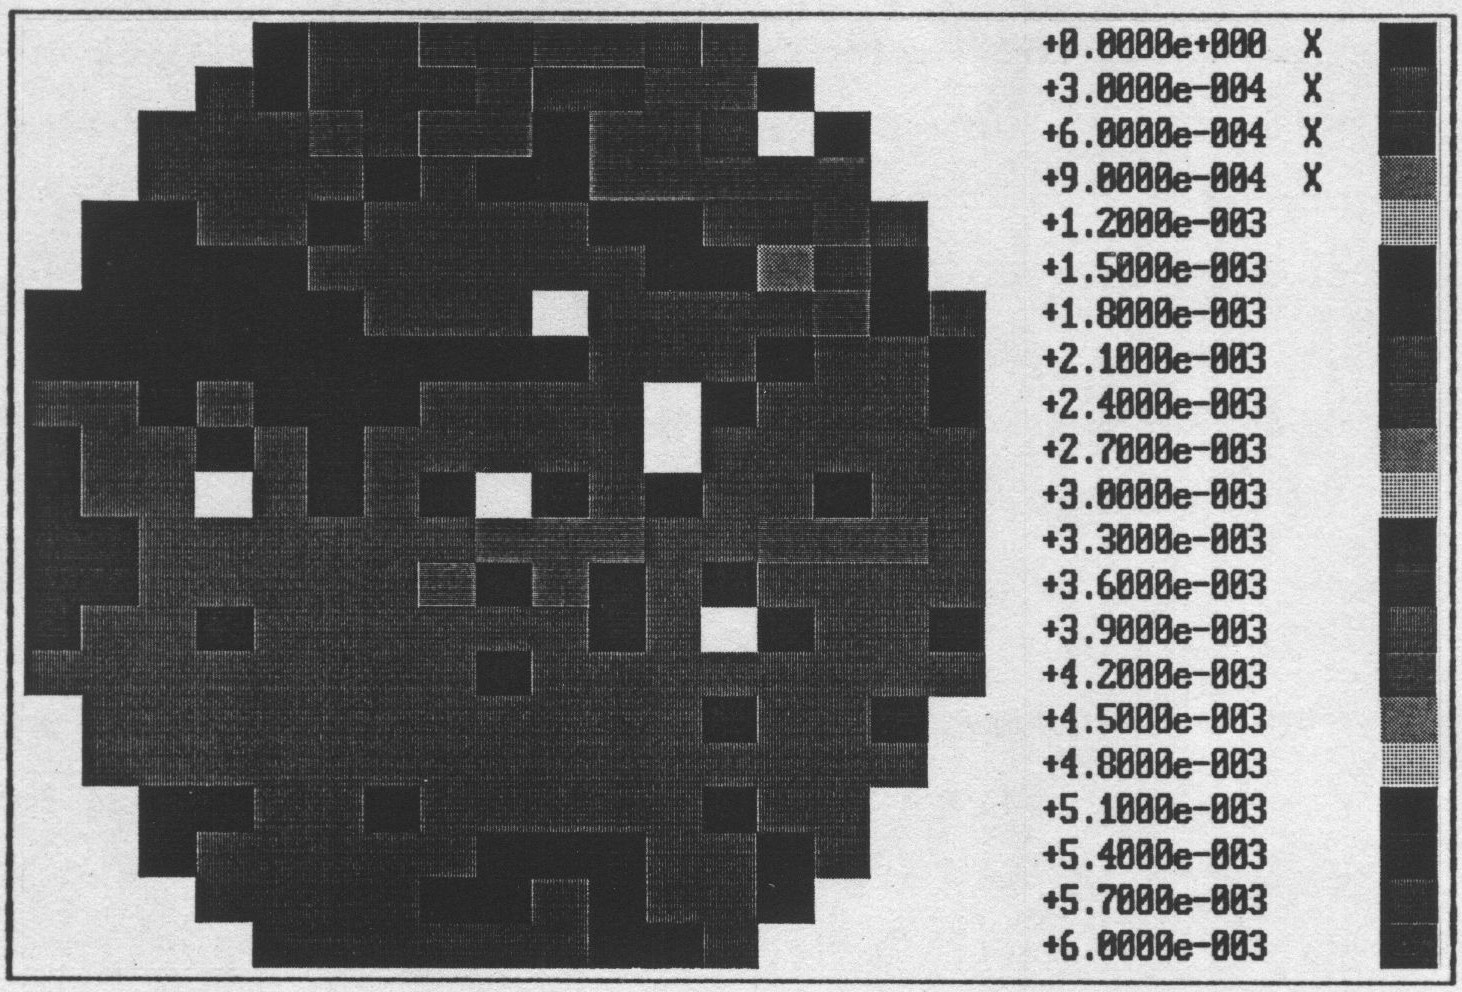
\includegraphics{Figures/fig-6-6.eps}
\captionsetup{justification=raggedright, singlelinecheck=false}
\caption[Plošné rozloženie generačného času života minoritných nosičov
  náboja]{Plošné rozloženie generačného času života minoritných
  nosičov náboja pre oblasť polovodiča od $0.9 \mu m$ do $1.3
  \mu m$.}
\label{fig:6.6}
\end{figure}

\begin{thebibliography}{}
\bibitem[6.1]{6.1}
Ludwig R.: Methoden der Fehler und Ausgleichrechnung. VEB Berlin 1969. s.103.
\end{thebibliography}
 
% Chapter 7
\chapter{Experimental results.}\label{Chapter7}
\lhead{Chapter 7. \emph{Experimental Results}}

The final experiment was performed on MOS structures with
inhomogeneous depth profile of the dopant impurities, which was
created by a process ion implantation with different doses in an
N-type silicon single crystal with orientation [100].

Prior to technological processing, the homogeneity was tested of the
specific resistivity of the used silicon wafers by means of a device
Prometrix OmniMap RS35, which uses a four-point method to determine
surface specific resistivity. Table~\ref{tab:7.1} shows the mean
values of the specific resistivity $\overline\rho$ and the standard
deviation of $\delta\rho$ expressed in absolute and relative values.

\begin{table}[h!]\centering
  \begin{tabular}{c c c c c c c c}
    No. & $\overline\rho[\Omega cm]$ & $\delta\rho[\Omega cm]$ & $\delta\rho[\%]$ &
    No. & $\overline\rho[\Omega cm]$ & $\delta\rho[\Omega cm]$ & $\delta\rho[\%]$\\
    \hline% chktex-file 44
    1 & 4.3319 & 0.1223 & 2.822 & 11 & 4.5706 & 0.1658 & 3.627\\
    2 & 4.2733 & 0.1204 & 2.817 & 12 & 4.4762 & 0.1860 & 4.155\\
    3 & 5.1040 & 0.3405 & 6.671 & 13 & 4.3332 & 0.1265 & 2.290\\
    4 & 4.6276 & 0.2080 & 4.494 & 14 & 4.8422 & 0.3573 & 7.380\\
    5 & 4.7697 & 0.1824 & 3.824 & 15 & 4.5917 & 0.1741 & 3.791\\
    6 & 4.8007 & 0.2340 & 4.873 & 16 & 4.8134 & 0.2590 & 5.380\\
    7 & 4.2500 & 0.1436 & 3.378 & 17 & 4.4025 & 0.1527 & 3.468\\
    8 & 4.8259 & 0.3163 & 6.554 & 18 & 4.3591 & 0.1290 & 2.960\\
    9 & 4.2853 & 0.1418 & 3.308 & 19 & 4.3877 & 0.1349 & 3.074\\
    10 & 4.2954 & 0.1113 & 2.592 & 20 & 4.5416 & 0.1618 & 3.563\\
  \end{tabular}
  \caption[Mean and standard deviation of specific resistance of the
    tested silicon wafers before technological processing]{Mean value
    and standard deviation of the specific resistance of the tested
    silicon wafers before technological processing.}\label{tab:7.1}
\end{table}

The Prometrix OmniMap RS35 device measured the the specific resistance
value at 81 points on each plate. At Figure~\ref{fig:7.1} and
Figure~\ref{fig:7.2} we present graphical representation of the
specific resistance distribution, which is also the output of of the
measurement of the above device. The points at which the specific
resistance are indicated in Figure~\ref{fig:7.1} by $+$ or $-$
depending on whether the value of the specific resistance at that
point lay above, or below the mean value, which is shown by the
thicker line.  An idea of the quantitative distribution of the
specific resistance can be can be obtained from the three-dimensional
figure~\ref{fig:7.2}.

The sequence of the main technological operations for the formation of
MOS structures on the substrates mentioned above was as follows

\begin{itemize}
\item formation of a $100 \nu m$ thick gate oxide
\item implantation of $P^{31}$ with energy $120 keV$ and doses 0.6,
  1.0, 2.0, 4.0, 5.0, 6.0, 7.0, 8.0, 20.0, 60.0 $\times 10^{15}
  m^{-2}$ under angle $7\degree$
\item activation at temperature $1050 \degree C$ with time course: 15
  min.\ start-up, 30 min.\ activation, 40 min.\ cooling
\item Al vaporization on both sides of the silicon wafer
\item lithography process to create CV mask
\item sintering of Al FG at $460 \degree C$ for 20 min.
\end{itemize}

20 silicon wafers with a diameter of 4 inches, two each time with the
same implantation dose. In the process of data collection 304
structures were tested on each silicon wafer, with the area of one
structure was $0.81 \times 10^{-6} m^{-2}$. At Figure~\ref{fig:7.3}
shows the concentration profiles of the dopants for each implantation
dose. Shown waveforms represent the mean over all $N(x)$ dependencies,
that have been determined on the test plate. From each batch, the
Figure~\ref{fig:7.3} only one silicon wafer is shown.

\newpage
\begin{figure}[h!]\centering
  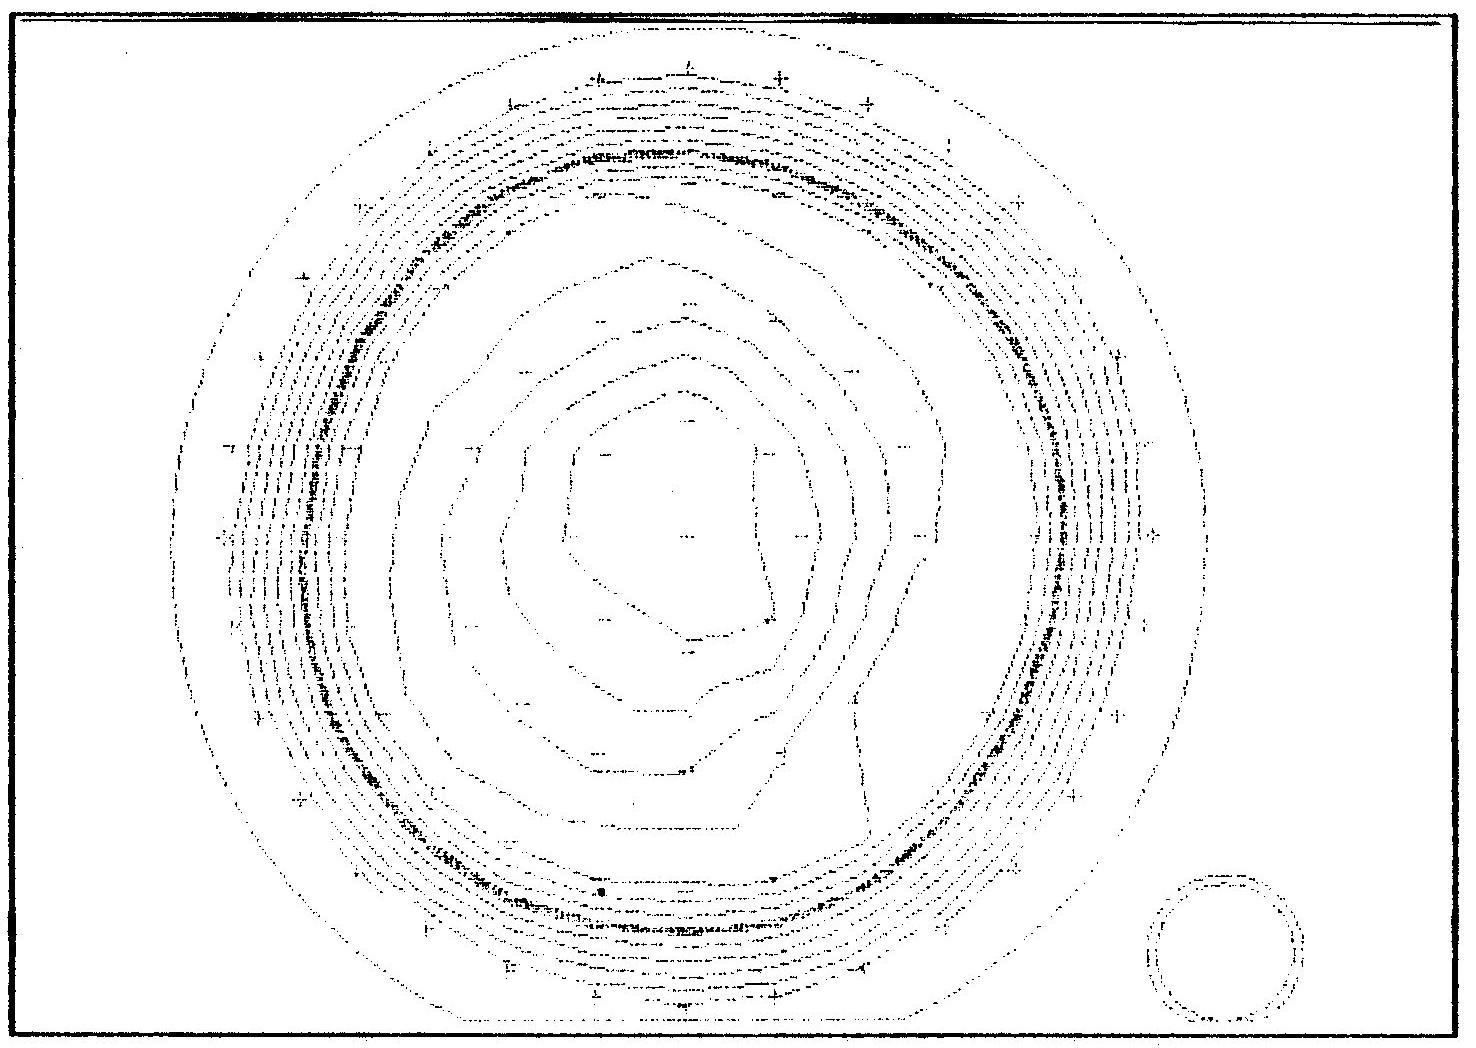
\includegraphics{Figures/fig-7-1.eps}% chktex-file 8
  \caption[Area distribution of surface specific resistance of silicon
    wafer No.16]{Surface Specific Resistivity Distribution specific
    resistivity of silicon wafer No.16.}\label{fig:7.1}
\end{figure}

\begin{figure}[h!]\centering
  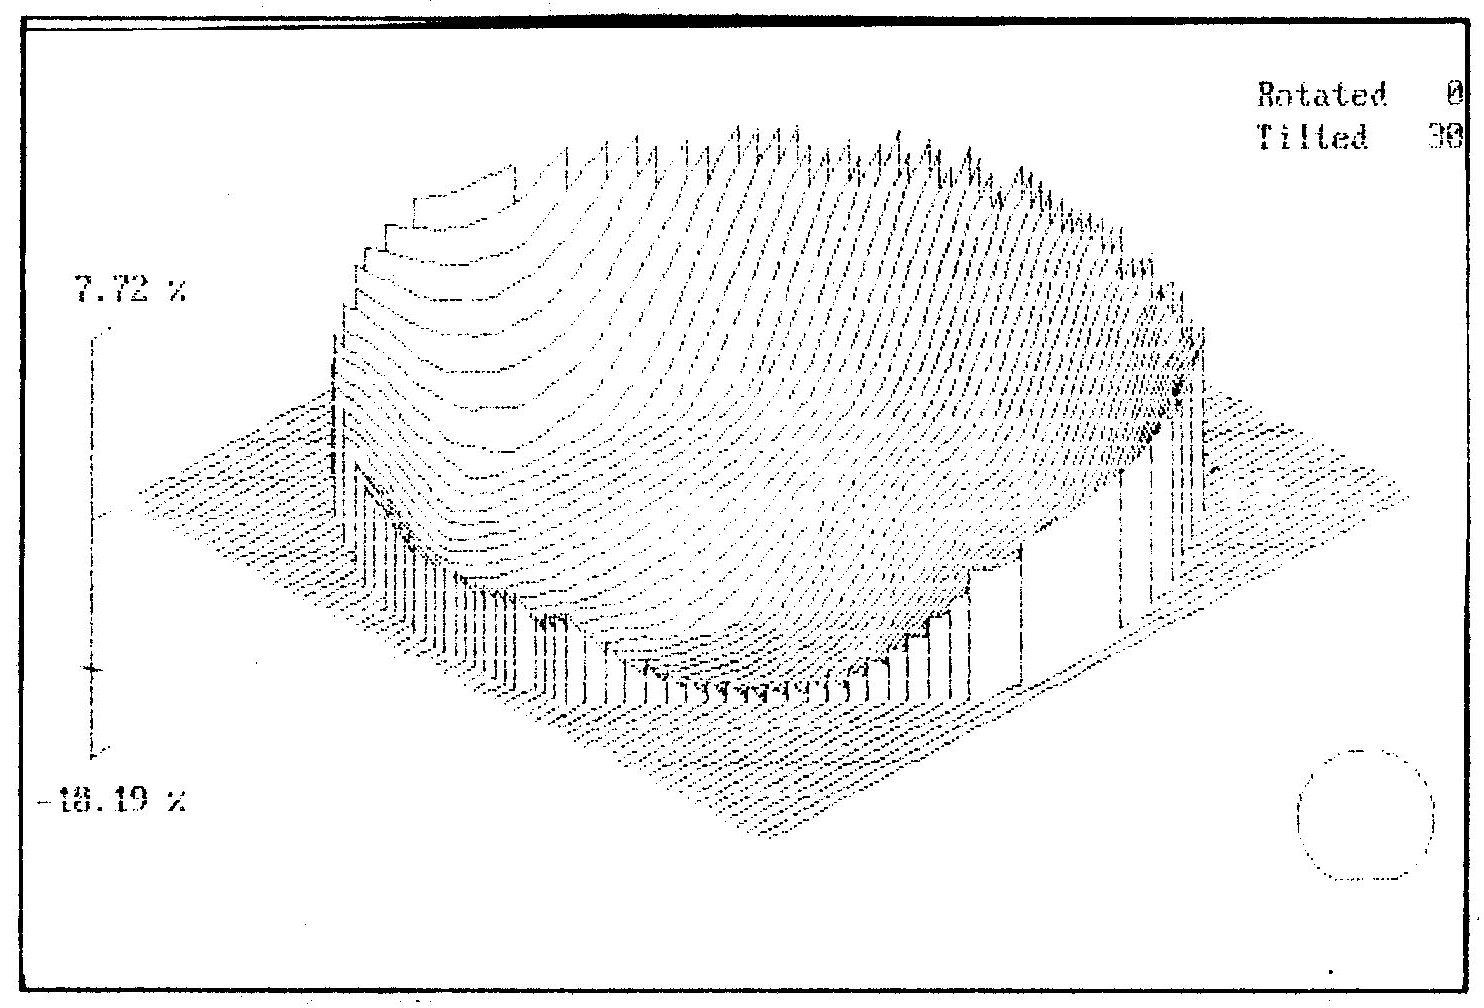
\includegraphics{Figures/fig-7-2.eps}
  \caption[Area distribution of surface specific resistance of silicon
    wafer No.16]{Surface Specific Resistivity Distribution of silicon
    wafer No.16.}\label{fig:7.2}
\end{figure}

\newpage
\begin{figure}[h!]\centering
  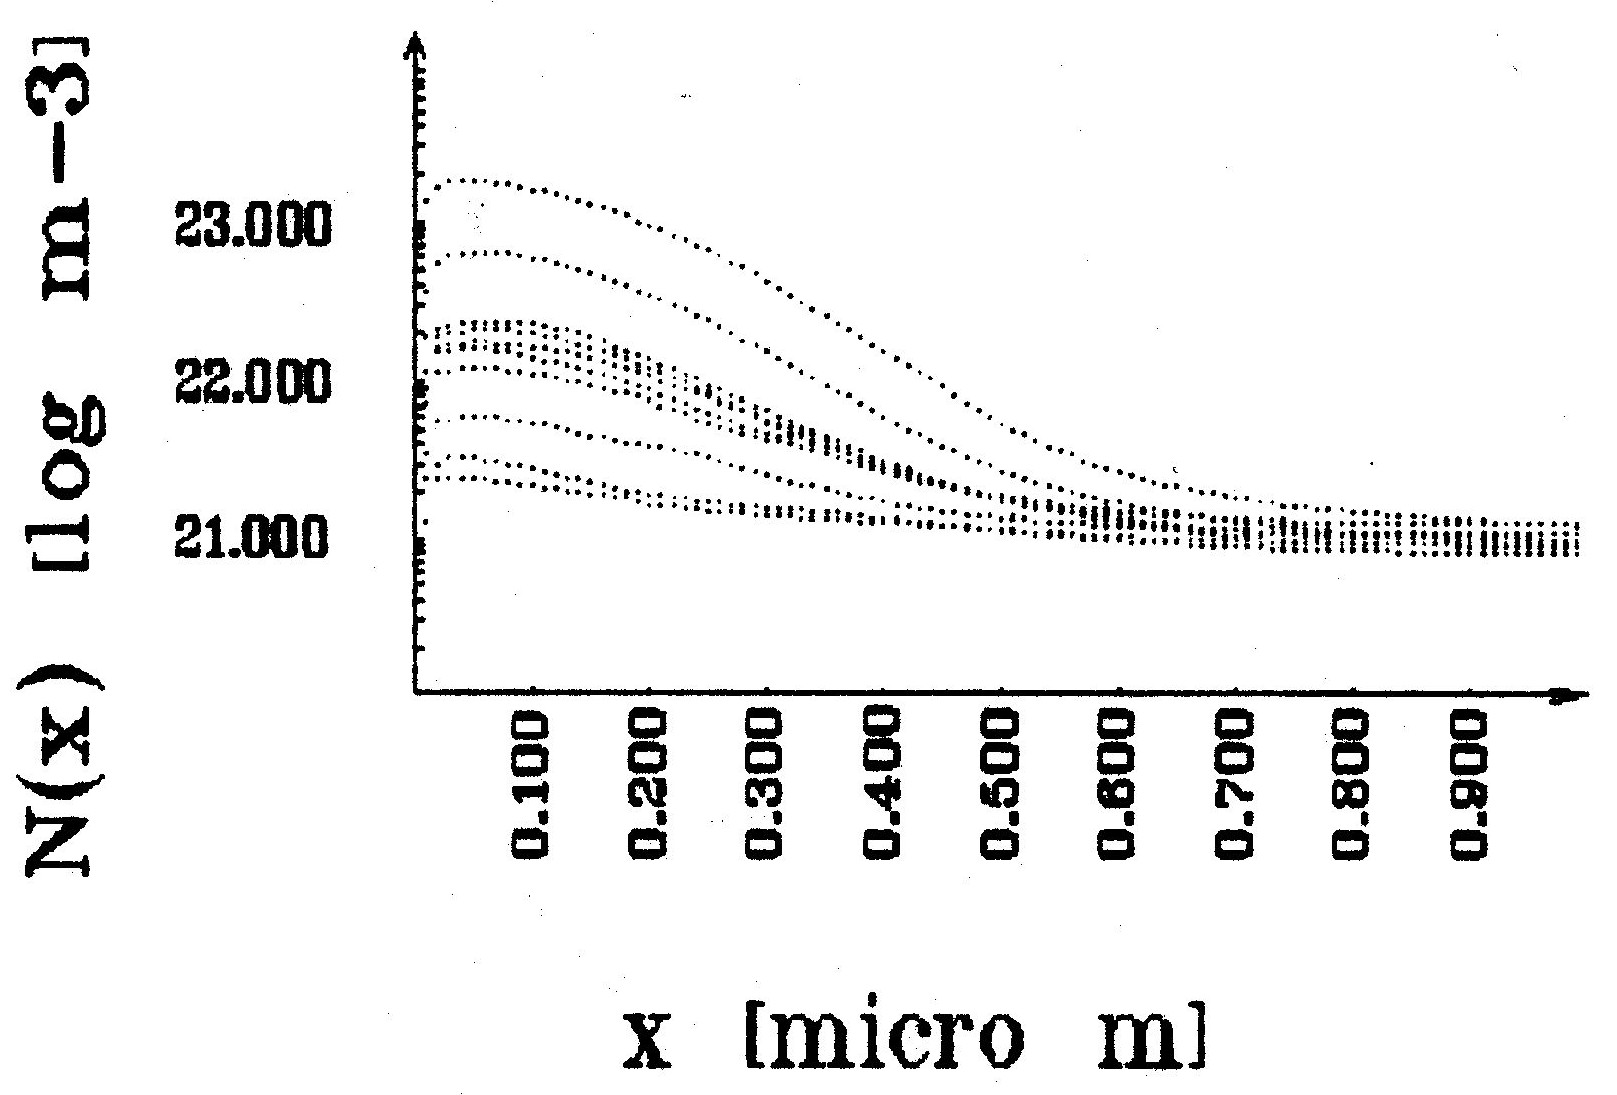
\includegraphics{Figures/fig-7-3.eps}
  \caption[Depth profile of tangents]{Depth profile of the interfering
    impurities in the subsurface region of the semiconductor formed by
    ion implantation with doses of $0.6, 1.0, 2.0, 4.0, 5.0, 6.0, 7.0,
    8.0, 20.0, 60.0 \times 10^{15} m^{-2}$. Shown are the $N(x)$
    waveforms represent the mean of the waveforms measured at 304 MOS
    structures of each silicon wafer.}\label{fig:7.3}
\end{figure}
% OBR27.BIT

\begin{table}[h!]\centering
  \begin{tabular}{c c c c}
    No. & ${D_{i}}{10}^{15}[m^{-2}]$ & $\overline{D}{10}^{15}[m^{-2}]$ & $\delta{D}{10}^{15}[m^{-2}]$\\
    \hline
    1 & 0.6 & 0.39 & 0.02\\
    3 & 1.0 & 0.59 & 0.08\\
    5 & 2.0 & 1.20 & 0.06\\
    7 & 4.0 & 2.67 & 0.09\\
    9 & 5.0 & 3.40 & 0.13\\
    11 & 6.0 & 4.07 & 0.13\\
    13 & 7.0 & 4.72 & 0.14\\
    15 & 8.0 & 5.49 & 0.09\\
    17 & 20.0 & 14.41 & 0.35\\
    19 & 60.0 & 42.63 & 0.21\\
  \end{tabular}
  \caption[Implantation dose $D_{i}$]{Implantation dose $D_{i}$, the
    calculated mean value of the implanted and activated ions in the
    semiconductor $\overline D$ and its standard deviation $\delta D$
    on the silicon wafer.}\label{tab:7.2}
\end{table}

Table~\ref{tab:7.2} contains the numerical values of the implant dose
entered during the implantation process $D_{i}$, the mean value of
$\overline D$ and the standard deviation of $\delta D$ of the doses
calculated by the procedure described in section~\ref{sec:6.1}.

To check the reproducibility of the implantation process, the
concentration profiles on 3 additional silicon wafers were
measured. In the Table~\ref{tab:7.3} are the implantation dose values
for the three pairs of silicon wafers that were implanted with the
same dose.

\newpage
\begin{figure}[h!]\centering
  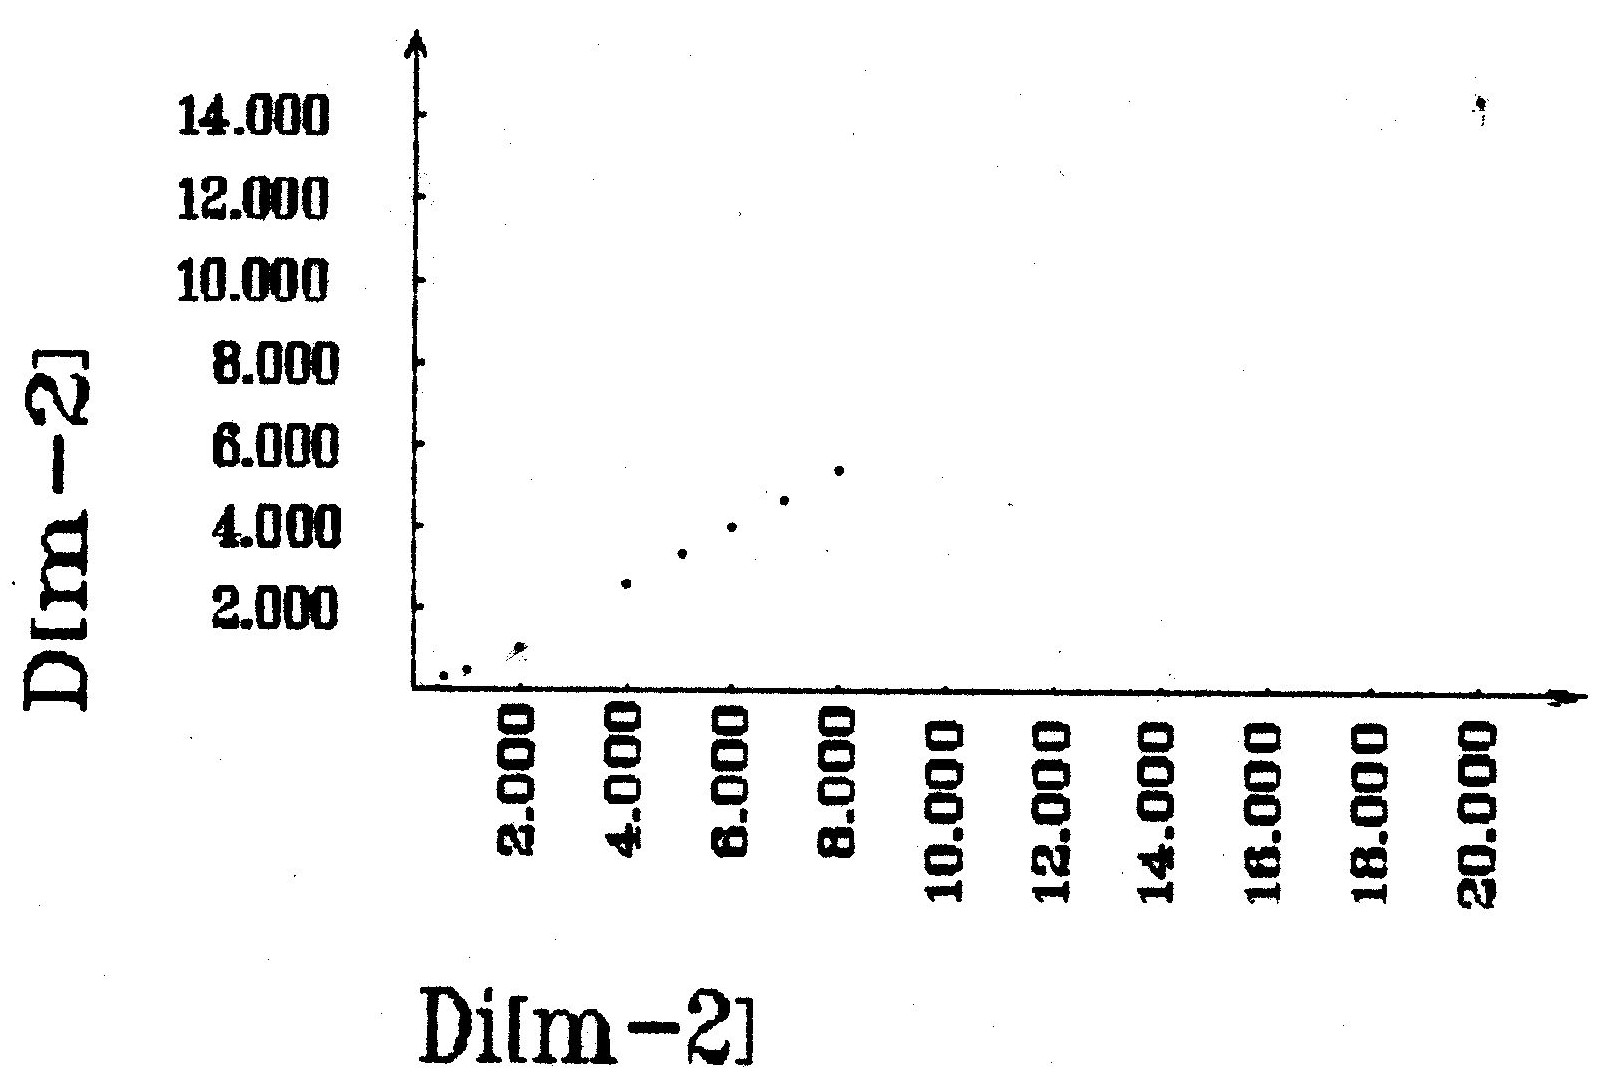
\includegraphics{Figures/fig-7-4.eps}
  \caption[Dependence of mean value
    $\overline{D}=E(\int(N(x)-N_{b})dx)$ on the implanted ion dose
    $D_{i}$]{Dependence of the mean value
    $\overline{D}=E(\int(N(x)-N_{b})dx)$ from the implanted ion dose
    $D_{i}$. Values shown are of order $10^{15}$.}\label{fig:7.4}
\end{figure}
%OBR29.BIT
 
\begin{table}[h!]\centering
  \begin{tabular}{c c c c}
    No. & $D_{i} 10^{15} [m^{-2}]$ & $\overline D 10^{15} [m^{-2}]$ & $\delta D 10^{15} [m^{-2}]$\\
    \hline
    9 & 5.0 & 3.40 & 0.13\\
    10 & 5.0 & 3.56 & 0.06\\
    11 & 6.0 & 4.07 & 0.13\\
    12 & 6.0 & 4.03 & 0.12\\
    15 & 8.0 & 5.49 & 0.09\\
    16 & 8.0 & 5.46 & 0.08\\
  \end{tabular}
  \caption[Implantation dose $D_{i}$]{Implantation dose $D_{i}$, the
    calculated mean of the dose of implanted and activated ions in the
    semiconductor $\overline D$ and its standard deviation $\delta D$
    on the silicon wafer.}\label{tab:7.3}
\end{table}

As can be seen from Table~\ref{tab:7.2} and~\ref{tab:7.3}, the
calculated implant dose is always less than the dose entered in the
process implantation. This is due, however, to the fact that the time
of implanted ions is trapped in the oxide layer, and yet incomplete
activation of the implanted ions in the semiconductor. In order to
determine the dependence between the specified and calculated dose, we
calculated by linear regression the coefficient $b$ of the relation

\begin{equation}\label{eq:7.1}
  \overline D = bD_{i}
\end{equation}

which had a value of $b = 0.71$ and we also plotted the dependence
$\overline D = f(D_{i})$ in Figure~\ref{fig:7.4}.

By doing so, we found that the original dose that was implanted became
electrically active $71\%$ of the implanted ions.

To determine the degree of dependence between the implanted dose and
the amount of electrically active impurities in the semiconductor,
which were implanted, we calculated the correlation coefficient
between these quantities. We used the relationship

\begin{equation}\label{eq:7.2}
  R(X,Y) = \frac{E([X-E(X)][Y-E(Y)])}{D(X)D(Y)}
\end{equation}

, which is given for example in~\cite{7.1}. In the
equation~\ref{eq:7.2} X and Y represent random variables, E represents
the mean and D denotes the standard deviation. This way we have
obtained the value of of the correlation coefficient

\centerline{$R(D_{i}, \overline{D}) = 0.99$}

taking the values of $D_{i}$ and $\overline{D}$ as realizations of the
random variable and we used all the values given in
Table~\ref{tab:7.2} and~\ref{tab:7.3}. It may be noted that in the
theory of probability the theorem is proved that $\rvert R(X,Y)\rvert
= 1$ precisely if, with probability 1, is valid

\centerline{$Y = a + b X$}

It follows that the dependence between the values of $D_{i}$ and
$\overline D$ is linear in this case.

\newpage
Using a professional program, purchased by Tesla Piešťany, to
simulate the process of ion implantation, the waveforms were
calculated of impurity concentration for doses of 0.6, 5.0 and 60.0
$\times10^{15}m^{-2}$.  The concentration profile waveforms were
simulated based on the specified implantation conditions using the
Pearson IV\@ method.  A comparison of the measured and simulated
impurity concentration waveforms is shown in Figure~\ref{fig:7.5}.

\begin{figure}[h!]\centering
  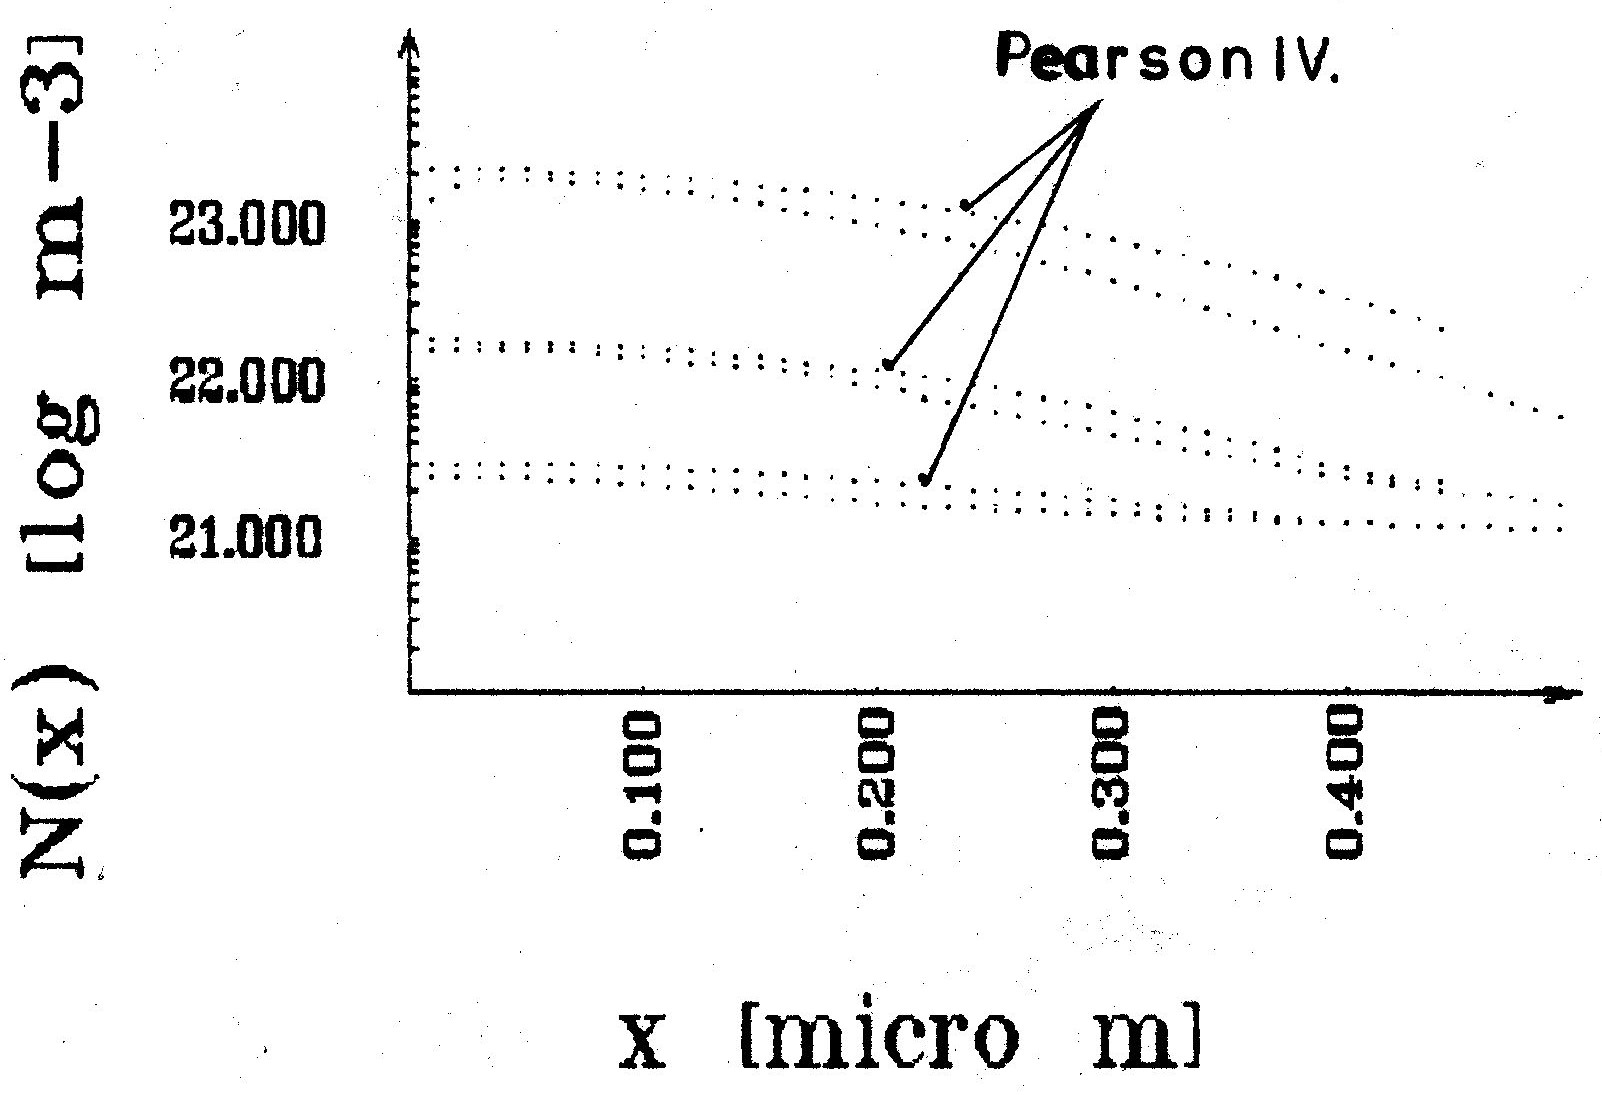
\includegraphics{Figures/fig-7-5.eps}
  \caption[Comparison of the mean values of the measured waveforms
    $N(x)$ and simulated using the Pearson IV method]{Comparison of
    means values of the measured $N(x)$ and simulated $N(x)$ waveforms
    Pearson IV for doses $0.6, 5.0, 60.0 \times 10^{15}
    m^{-2}$.}\label{fig:7.5}
\end{figure}
% OBR33.BIT

In the process of calculating the depth profiles of the intervening
admixtures, we simultaneously also determined the values of the
stresses of the aligned bands $V_{fb}$ for each MOS\@ structure
tested. Using a separate program that determines based on the data
contained in a given data file, the mean value and standard deviation
of the stored parameters, we calculated the mean of $\overline V{fb}$
and the standard deviation of $\delta V{fb}$. At the same time, using
the same procedure, we determined the values of $\overline h_{ox}$ and
$\delta h_{ox}$, which are for each silicon slabs are given in
Table~\ref{tab:7.4}.

It can be seen from the table~\ref{tab:7.4} that the values of
$\overline V_{fb}$ are related to the mean values of the oxide layer
thickness $\overline h_{ox}$, so we have shown this dependence in
Figure~\ref{fig:7.6}.

\newpage
\begin{figure}[h!]\centering
  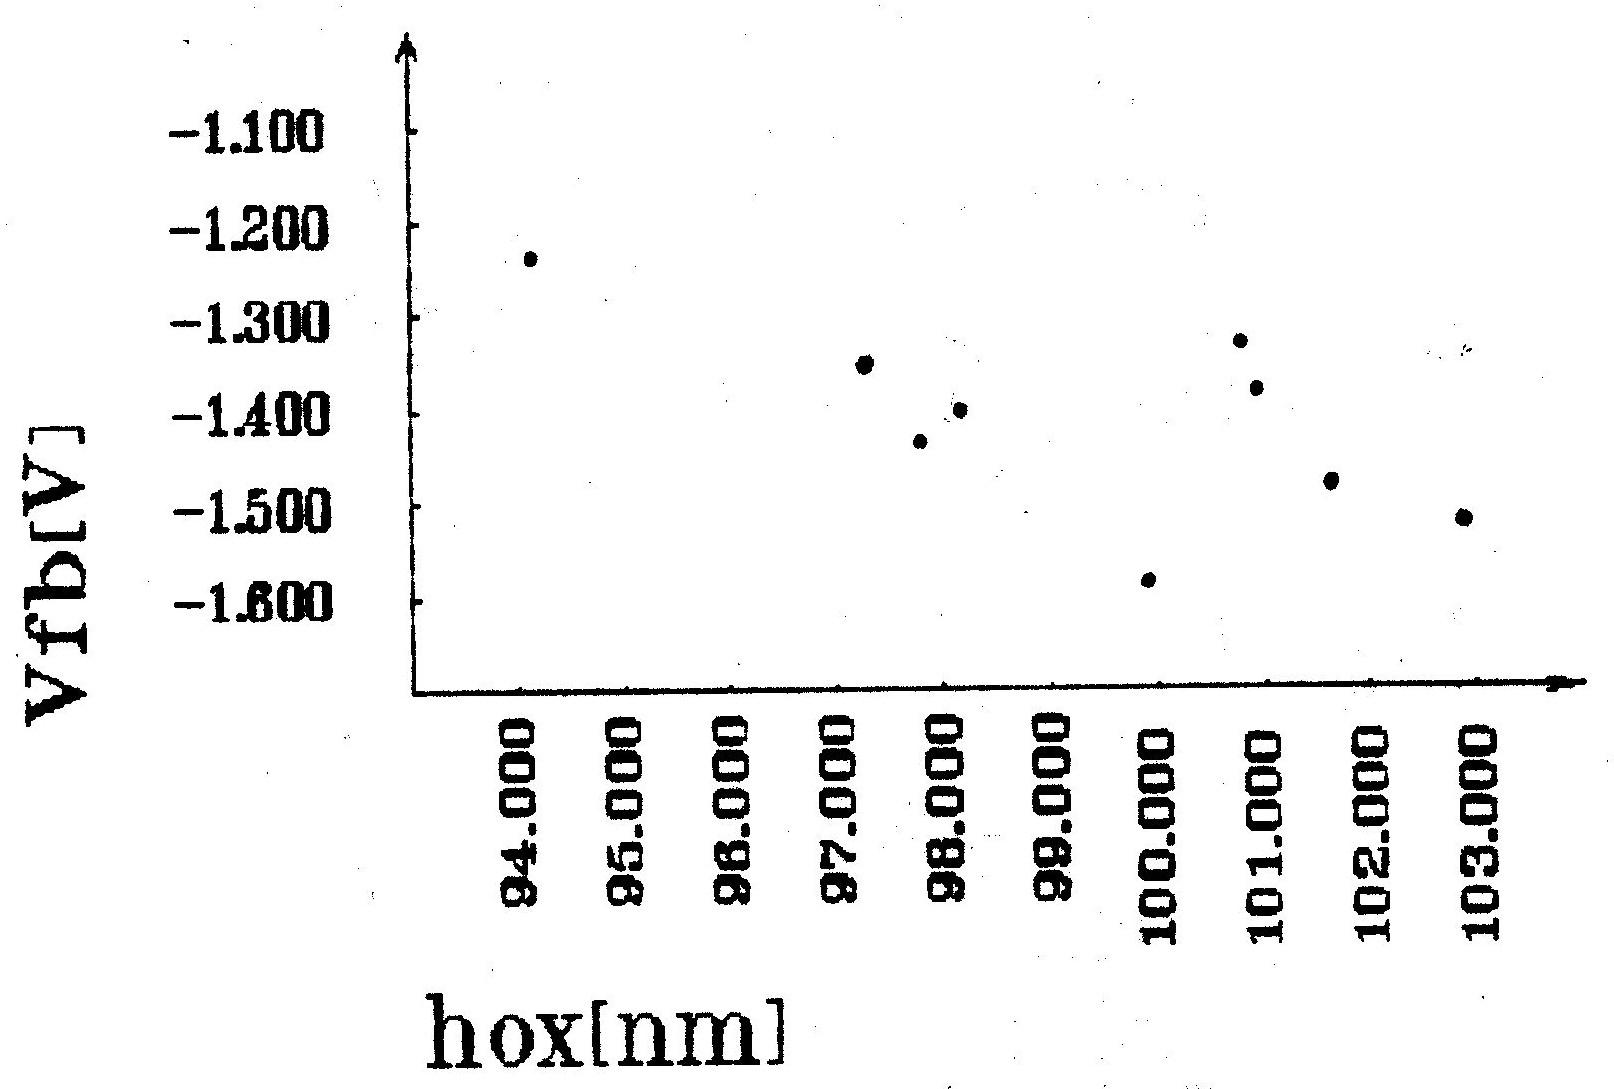
\includegraphics{Figures/fig-7-6.eps}
  \caption[Dependence of the mean value of $\overline V_{fb}$ on the
    mean value of the oxide layer thickness $\overline
    h_{ox}$]{Dependence of the mean value of $\overline V_{fb}$ on the
    mean value of the thickness of the oxide layer $\overline h_{ox}$
    for silicon wafers number 1, 3, 5, 7, 9, 11, 13, 15 and
    17.}\label{fig:7.6}
\end{figure}
% OBR28.BIT

\begin{table}[h!]\centering
  \begin{tabular}{c c c c c}
    No. & $\overline V_{fb} [V]$ & $\delta V_{fb} [V]$ & $\overline h_{ox} [nm]$ & $\delta h_{ox} [nm]$\\
    \hline
    1 & -1.24 & 0.07 & 94.14 & 0.89\\
    3 & -1.43 & 0.07 & 97.79 & 0.80\\
    5 & -1.35 & 0.08 & 97.26 & 0.28\\
    7 & -1.40 & 0.09 & 98.15 & 0.35\\
    9 & -1.52 & 0.09 & 102.85 & 0.53\\
    11 & -1.48 & 0.08 & 101.65 & 0.32\\
    13 & -1.38 & 0.08 & 100.94 & 0.41\\
    15 & -1.33 & 0.07 & 100.80 & 0.16\\
    17 & -1.59 & 0.08 & 99.93 & 0.22\\
    19 & -2.43 & 0.16 & 99.67 & 0.19\\
  \end{tabular}
  \caption[Mean and standard deviation of the voltage of the aligned
    strips and oxide thickness]{Mean and standard deviation of aligned
    strip stress and oxide thickness.}\label{tab:7.4}
\end{table}

Correlation coefficient value

\centerline{$R(\overline V_{fb} ,\overline h_{ox}) = -0.78$}

agrees with the theoretical relationship defining the dependence of
$V_{fb}$ on the magnitude of the breakdown charge in the oxide layer
and at the interface $Si-SiO_{2}$ $Q_{dc}$ and on the magnitude of the
oxide layer capacitance $C_{ox}$

\begin{equation}\label{eq:7.3}
  V_{fb}  = \varphi_{ms} + \frac{Q_{dc}}{C_{ox}}
\end{equation}

where $\varphi_{ms}$ represents the difference in output potentials
between the semiconductor and the metal.

For linear regression coefficients

\centerline{$V_{fb}  = a + b h_{ox}$}

we obtained the values

\centerline{$a = 5.48 \times 10^{-3} \qquad b = -1.41 \times 10^{7}$}

The interface trap density was determined on four silicon wafers
$Si-SiO_2$ $D_{it}$. As can be seen from Table~\ref{tab:7.5}, the mean
values of $\overline D_{it}$ are in the region of $2.0-5.0\times
10^{14}$, which speaks for the good quality of the $Si-SiO_{2}$
interface.

The crystal quality is indicated by the magnitude of the generation
time of the minority charge carriers. In order to compare the quality
of the crystal for individual slabs, we determined on each silicon
slab the area distribution of $³tau_{g}$ at depths ranging from $0.9$
to $1.3 m$. For all slabs we then determined the mean value of
$\overline\tau_{g}$ and the standard deviation of $\overline\tau_{g}$
deviation of $\delta\tau_{g}$, the values of which are given in
Table~\ref{tab:7.6}. The values of $\overline\tau_{g}$ range in
between $0.41\ and\ 2.25 ms$, indicating a high quality of the
substrate. At the same time, it can be seen from Table~\ref{tab:7.6}
that the values of $\overline \tau_{g}$ are randomly varying and
cannot be found dependence on the other previously mentioned
parameters.

\begin{table}[h!]\centering
  \begin{tabular}{c c c}
    No. & ${\bar{D_{it}}}[m^{-2}eV^{-1}]$ & $\delta D_{it}[m^{-2}eV^{-1}]$\\
    \hline
    3 & $4.42 \times 10^{14}$ & $0.25 \times 10^{14}$\\
    7 & $2.60 \times 10^{14}$ & $0.15 \times 10^{14}$\\
    9 & $2.74 \times 10^{14}$ & $0.15 \times 10^{14}$\\
    12 & $3.55 \times 10^{14}$ & $0.16 \times 10^{14}$\\
  \end{tabular}
  \caption[Mean and standard deviation of trap densities of the
    $Si-SiO_{2}$ interface at the center of the forbidden band.]{Mean
    value and standard deviation of the trap density of the
    $Si-SiO_{2}$ interface at the centre of the forbidden
    band.}\label{tab:7.5}
\end{table}

\begin{table}[h!]\centering
  \begin{tabular}{c c c}
    No. & ${\bar{\tau_{g}}}[ms]$ & $\delta\tau_{g}[ms]$\\
    \hline
    1 & 1.93 & 0.12\\
    3 & 1.48 & 0.09\\
    5 & 1.84 & 0.09\\
    7 & 1.67 & 0.10\\
    10 & 1.95 & 0.09\\
    12 & 0.41 & 0.02\\
    15 & 1.74 & 0.09\\
    17 & 2.25 & 0.14\\
  \end{tabular}
  \caption[Mean and standard deviation of generation time of life of
    minority carriers of charge]{Mean and standard deviation of the
    generational lifetime of minority carriers of
    charge.}\label{tab:7.6}
\end{table}


\begin{thebibliography}{}
\bibitem[7.1]{7.1}
  Renyi A.: Theory of Probability. Academia Prague 1972.
\end{thebibliography}
 
% Chapter 8
\chapter{Summary of results with new findings.}\label{Chapter8}
\lhead{Chapter 8. \emph{Summary of results with new findings}}
%----------------------------------------------------------------------

The dissertation presents the results obtained by investigating the
parameters of MOS structures with inhomogeneous distribution of
impurities in the subsurface region of the semiconductor. Since in our
country there has not been so far this problem has been
comprehensively addressed in our country, it was necessary to
summarize the current knowledge in this field, to master the
methodology of measurement and evaluation of parameters and to
implement them practically. The practical side consisted of the
implementation of individual capacity methods and the creation of a
complex workplace for measurement and evaluation of the area
distribution parameters of MOS structures with with a view to further
use for the investigation of correlations between individual
parameters, or between the parameters of other test structures or
technological procedures of planar technology.

The dissertation has produced the following results:

\begin{enumerate}

% 1
\item We have solved the one-dimensional Poisson equation for
  inhomogeneously doped semiconductor substrate and calculated the
  theoretical CV dependences of the MOS\@ structure. Numerical
  solution of the Poisson equation made it possible to obtain
  information about the physical processes in the structure MOS in the
  process of CV dependence measurements and allowed verification of
  the used approximations in the calculation of the concentration
  profiles.

%2
\item In addition to the standard high-frequency and quasi-static CV
  methods method, we implemented a procedure for measuring MOS
  structures by QC method, where the needed:

  \begin{itemize}
  \item design and implement a fixture for the location of the measured sample and
    air condenser
  \item minimise leakage currents and parasitic capacitances
  \item select appropriate procedures for determining parasitic capacitances
  \item to develop software for data acquisition and processing.
  \end{itemize}

  As has been demonstrated during the implementation of the method, as
  well as during subsequent experiments, the implementation of the QC
  method requires the development of a thorough measurement
  workstation with an emphasis on minimizing leakage currents and
  parasitic capacitances.

%3
\item To measure the generation lifetime of minority charge carriers
  we have implemented the constant width OPN (CCT) method, which
  allows efficient evaluation of the quality of semiconductor
  substrates for high values of $\tau_{g}$. In the design of the
  control program, we designed and implemented an algorithm to
  maintain constant non-equilibrium capacitance of the MOS structure
  and to measure the dependence $V_{g}(t)$.

%4
\item All methods used (HF, LF, QC and CCT) were automated using a PC
  AT personal computer with a PCIIA interface, while the it was
  necessary to master the IMS-2 bus control and to make efficient use
  of the autonomous capabilities of the instruments used. To
  investigate the area distribution of the parameters of the MOS
  structures on the silicon wafer, we developed a software package
  consisting of approximately 40 programs, that perform data
  acquisition, processing and parameter determination of MOS
  structures\@ At the same time, programs are available for displaying
  the results obtained. A brief overview of the developed programs,
  which are used for the collection, processing and display of areal
  distribution data parameters of MOS structures is given in
  Appendix~\ref{app:AppendixH}.

%5
\item When calculating the concentration profiles of the dopant
  impurities in the subsurface region of the semiconductor, we
  applied:

  \begin{itemize}
  \item correction to the deep depletion approximation at the surface
    semiconductor
  \item correction with respect to the trap density of the $Si-SiO_{2}$ interface
  \item calculation of the OPN region width using the waveform approximation
    of the electric potential in the semiconductor
  \item calculation of the spatial distribution of dopant atoms from
    the concentration profile of the major charge carriers.
  \end{itemize}

%6
\item We have verified the suitability of the approximations used by
  solving the Poisson equation and calculating the concentration
  profile of the major charge carriers from the theoretical CV
  dependence. Here it was shown that for the determination of the
  concentration profiles of the implanted impurities tested silicon
  wafers in the final experiment is the use of the above approximation
  is appropriate.

%7
\item For different implantation doses ranging from $0.6 \times
  10^{15}$ to $60.0 \times 10^{15} m^{-2}$ we determined on 10 silicon
  wafers $N(x)$ concentration profiles on approximately 300 structures
  MOS of each tested wafer and calculated their mean values. At the
  same time, we determined the mean value of the dose fraction of the
  implanted ions that became electrically active in $D_{a}$
  semiconductor. It turned out that the dependence between the dose
  $D_{i}$ implantation and the amount of electrically active,
  implanted $D_{a}=f(D_{i})$ is linear, as inferred from the value of
  of the correlation coefficient $R(D_{i},D_{a})=0.99$.  Linear
  regression of the dependence $D_{a}=f(D_{i})$, we found that from
  the original implanted dose entered the semiconductor and became
  electrically active $71\%$ of the ions. The above methodology can be
  used to control the process implantation and was developed based on
  the request of Tesla Piešťany.

%8
\item The calculated concentration profiles were verified by
  simulation technological process of implantation using Pearson IV
  function. Z comparison of the results obtained by capacitance
  measurements and simulation show a small difference, which may be
  due to the fact that in the post-implantation heat treatment process
  were not all implanted ions were activated. However, the differences
  found are minimal. A methodology has been developed to track the
  area distribution of the depth profiles of the dopant impurities
  within the boundaries of the of applicability of the capacitance
  method with the ability to track the areal distribution at arbitrary
  depths below the semiconductor surface. Based on experimental
  results, it can be concluded that the implantation process was
  reproducibly performed on 4 inch silicon substrates with high
  homogeneity of the impurity distribution, thus verifying the quality
  of of the implantation device.


%9
\item Previous results, obtained in the determination of depth
  concentration profiles have been used to investigate the properties
  of the interface $Si-SiO_{2}$ MOS structures with implanted
  substrate. For the analysis of these structures was used:

  \begin{enumerate}
  \item differential capacitance method, comparing HF and LF CV
    dependence of the MOS structure, calculating $\varphi_{s} (V_{g})$
    takes into account the depth profile of the impurities
  \item quasi-static CV method, based on comparison of experimental
    and theoretical CV dependence.
  \end{enumerate}

  A comparison of the results obtained by the two methods shows that
  the density of the $Si-SiO_{2}$ interface traps in the center of the
  forbidden band is practically does not differ. Both methodologies
  can be applied to the CV dependences determined by HF and
  quasi-static methods, or to the CV dependence of the MOS structure
  determined using the QC method. At the same time, we have mastered
  the procedure of determining the waveform surface potential
  $\varphi_s (V_g)$ using the QC method, or by integration of the LF
  CV dependence. To calculate the trap densities from the comparison
  experimental and theoretical CV dependence, we used the theoretical
  LF CV dependence determined by numerical solution of the Poisson
  equation for an inhomogeneous distribution of dopant impurities in
  the semiconductor.

%10
\item From the comparison of HF and LF CV dependence we determined the
  area distribution of the $Si-SiO_{2}$ interface trap densities. The
  mean value of trap density of the interface traps in the middle of
  the forbidden band of the tested plates ranged ranging from
  $2.6\ \times\ 10^{14}$ to $4.4\ \times\ 10^{14}m^{-2}eV^{-1}$. These
  values are at the lower limit of the resolving of the method used
  and are indicative of good interface quality $Si-SiO_{2}$ of the
  tested samples and at the same time the quality of the processing
  semiconductor substrates.

%11
\item In the final experiment, we used the CCT method to determine the
  area distribution of the mean value of $\tau_{g}$ on 8 silicon
  wafers in $0.9$ to $1.3 mm$ in depth, ranging from $0.41$ to $2.25
  ms$, indicating high substrate quality.
  \newline Advantage of the method used is that it evaluates
  $\tau_{g}$ from the generation current of minority charge carriers
  from the OPN region only and eliminates the influence of of the
  generation of minority charge carriers outside this region, which
  the reproducibility of the values of this parameter.
  \newline A correlation was found between the depth profile of the
  lifetime and the concentration profile of implanted
  admixtures. Achieved results indicate that the dominant mechanism in
  the studied samples, that determines the lifetime is the dispersion
  on ionised impurities. This also confirms that the semiconductor
  substrates investigated are high quality in terms of defects and
  therefore the scattering on them with respect to the scattering on
  ionised impurities is negligible.

%12
\item We have determined the areal distribution of the oxide layer
  thickness calculated from the capacity of the MOS structure in
  accumulation on 10 silicon wafers, from which shows inhomogeneities
  in the thickness of $SiO_{2}$ caused by uneven temperature
  distribution and turbulence of the oxidizing atmosphere in the tube
  of the oxidation furnace. \newline Mean values of $SiO_{2}$
  thickness on individual plates range from $94.14$ to $102.85 nm$,
  while in the technological process of manufacturing MOS structures
  was the required value of $100 nm$. \newline At the same time, the
  table of mean values shows that the oxide thickness is the lowest
  for silicon wafers, which were located at the front and back ends of
  the oxidation boat and the thickest oxide was formed in the middle,
  which was due to the splitting temperature in the oxidation
  tube. These findings are consistent with Bermann's model of the
  thermal oxidation mechanism.

%13
\item We have investigated the areal distribution of the stresses of
  the aligned $V_{fb}$ strips for 10 silicon wafers. The mean values
  of $V_{fb}$ on individual silicon wafers range from $-1.24$ to
  $-2.43 V$. Since the interface trapping charge for the studied
  plates is small, the scatter in the mean values of $V_{fb}$ may be
  due to the charge alkaline ions in the oxide.

%14
\item To solve the mathematical physics equations, we used the methods
numerical mathematics. We solved the differential equation of the
second order with initial conditions using the predictor-corrector
method with Runge-Kutta starting term, we searched for the roots of
the nonlinear equation by the tangent method, we used numerical
filters for smoothing and determining the derivatives of the
experimentally obtained data. They used NAG library functions for
approximation by cubic spline functions.

%15
\item We developed a system and data file structures that store the
  measured data and the determined parameters of the MOS structure,
  while we have taken into account the relationships between the
  different measurement methodologies and of parameter determination,
  contributing to greater efficiency of the programs and allowing
  further use of the obtained results.

\end{enumerate}
 
% Chapter 9
\chapter{Conclusions for the practice and development of the discipline.}\label{Chapter9}
\lhead{Chapter 9. \emph{Conclusions for the practice and development of the discipline}}
%- - - - - - - - - - - - - - - - - - - - - - - - - - - - - - - - - - - - - - - - - - -

In terms of the chosen objectives, a number of insights have been
achieved that have been applied in practice in the control of
technological procedures for the creation of semiconductor structures
by planar technology. In conclusion, the contributions of of the work
can be summarized in the following points:

\begin{enumerate}

% 1
\item Implementation of a complex automated workplace for the
  investigation of electrophysical properties of MOS structures with
  inhomogeneous with the possibility of monitoring the planar
  distribution of impurities:

  \begin{itemize}
  \item concentration profile of the dopant impurity $N(x)$ for
    different depths $x$
  \item of the depth profile of the lifetime $\tau_{g}(x)$ for
    different depths $x$
  \item of the $Si-SiO_{2}$ interface trap density $D_{it}(E_{c}-E)$
    for different energies in the forbidden band of the semiconductor
  \item of the voltages of the aligned strips $V_{fb}$
  \item of the oxide layer thickness $h_{ox}$.
  \end{itemize}

% 2
\item Selection of appropriate numerical methods and their use for the
  solution:

  \begin{itemize}
  \item one-dimensional Poisson equation
  \item nonlinear equation for determining the surface potential from
    OPN capacitance $C_{sc}$
  \item of smoothing and interpolation of experimentally determined data
  \item calculation of the derivative of experimentally determined data.
  \end{itemize}

% 3
\item Creation of software for experimental control measurements,
  processing and displaying the results of selected parameters of MOS
  structures with inhomogeneous distribution of impurities in the
  subsurface area of the semiconductor and their areal distribution.

% 4
\item Investigation of homogeneity of implantation process on 4-inch
  silicon wafers with a dose range from $0.6 \times 10^{14}$ to $60.0
  \times 10^{14} m^{-2}$ with respect to:

  \begin{itemize}
  \item depth profile of active impurities
  \item properties of the $Si-SiO_{2}$ interface
  \item depth profile of the generation lifetime of minority carriers
    of charge.
  \end{itemize}

% 5
\item A methodology for determining the implanted dose of
  impurities. Experimental results were verified by simulation of the
  technological process using Pearson IV function. Comparison of
  experimental and theoretical results show minimal difference. The
  proposed methodology for controlling the implanted dose is
  applicable in practice.

% 6
\item A correlation between the concentration profile was found
  between the concentration profile of dopants and the depth profile
  of the generation lifetime of minority charge carriers. The lifetime
  profile of high quality silicon substrates is not determined by the
  dispersion mechanism on random substrate defects, but only on the
  implanted impurities.

\end{enumerate}
 

%----------------------------------------------------------------------------------------
%	THESIS CONTENT - APPENDICES
%----------------------------------------------------------------------------------------
\addtocontents{toc}{\vspace{2em}} % Add a gap in the Contents, for aesthetics
\appendix % Cue to tell LaTeX that the following 'chapters' are Appendices
% Include the appendices of the thesis as separate files from the Appendices folder
% Uncomment the lines as you write the Appendices
% Appendix A

\chapter{Numerické riešenie Poissonovej rovnice} % Main appendix title

\label{app:AppendixA} % For referencing this appendix elsewhere, use \ref{AppendixA}

\lhead{Appendix A. \emph{Numerické riešenie Poissonovej rovnice}} % This is for the header on each page - perhaps a shortened title

Poissonovu rovnicu možno napísať v normalizovanom tvare (Dodatok
\ref{app:AppendixB})

\begin{equation}\label{eq:A.1}
{\frac{d^2u}{dx^2} = e^u - e^{2u_f-u} + \alpha(x) - 1} \qquad {x\ge0}
\end{equation}

Koncentrácie majoritných a minoritných nosičov náboja predstavujú prvé
dva členy na pravej strane rovnice. Koncentráciu substrátu a prímesí
predstavuje člen $\alpha(x)-1$. Uvedenú rovnicu budeme riešiť ako
diferenciálnu rovnicu druhého rádu s počiatočnými podmienkami, ktoré
získame následujúcou úvahou \cite{App.1}. Vo väčšine prípadov
nehomogénnej koncentrácie polovodiča možno nájsť hĺbku v polovodiči,
za ktorou môžeme považovať koncentráciu prímesí za konštantnú. Označme
túto hĺbku $x_1$ a určime ju z podmienky

\begin{equation}\label{eq:A.2}
{\alpha(x_1)  =  0.01}
\end{equation}

Potom pre $x\ge{x_1}$  môžeme zanedbať člen $\alpha(x)$

\begin{equation}\label{eq:A.3}
{\frac{d^2u}{dx^2} = e^u -  e^{2u_f-u}  - 1} \qquad {x\ge{x_1}}
\end{equation}

Vzťah \ref{eq:A.3} predstavuje
Poissonovu rovnicu pre homogénny polovodič, ktorú možno riešiť
analyticky s okrajovými podmienkami

\begin{equation}\label{eq:A.4}
u(\infty) = 0 \qquad \frac{du}{dx}\Big\rvert_{x=\infty} = 0
\end{equation}

aby sme dostali vzťah pre prvú deriváciu potenciálu

\begin{equation}\label{eq:A.5}
\frac{du}{dx} = - \frac{u}{|u|} \sqrt{2} \Big[e^u - e^{2u_f-u} - 1
  \Big]^{\frac{1}{2}} \qquad {x\ge{x_1}}
\end{equation}

Počiatočné podmienky pre riešenie rovnice \ref{eq:A.1} v oblasti
${0\leq{x}\leq{x_1}}$ potom tvorí voľne zvolený potenciál v bode $x_1$
a prvá derivácia potenciálu v bode $x_1$ vyjadrená vzťahom
\ref{eq:A.5}. Vhodnou volbou potenciálu v bode $x_1$ a opakovaným
numerickým riešením rovnice \ref{eq:A.1} z objemu po povrch polovodiča
dostaneme súbor priebehov potenciálu v polovodiči od akumulácie po
inverziu. Potrebujeme ešte poznať napätie hradla pre každý priebeh
potenciálu v polovodiči pri známej kapacite oxidovej vrstvy.  Pre
normálové zložky intenzity elektrického poľa na rozhraní oxidu a
polovodiča platí vzťah

\begin{equation}\label{eq:A.6}
\varepsilon_{ox}E_{ox} = \varepsilon_s{E_s}
\end{equation}

Ak označíme hrúbku oxidovej vrstvy $h_{ox}$, pre napätie hradla
dostaneme vzťahy

\begin{equation}\label{eq:A.7}
v_g = u_s + h_{ox}E_{ox}
\end{equation}

\begin{equation}\label{eq:A.8}
v_g = u_s - ku_{s}^{'} \qquad k =
h_{ox}\frac{\varepsilon_s}{\varepsilon_{ox}}
\end{equation}

kde $u_s$ je hodnota potenciálu na povrchu polovodiča a $u_{s}^{'}$
jej priestorová derivácia. Po odnormovaní sme tým získali priebeh
povrchového potenciálu ako funkciu napätia hradla (obrázok \ref{fig:1.2}). Pre
výpočet kapacity štruktúry MOS následovným vzťahom (Dodatok
\ref{app:AppendixC})

\begin{equation}\label{eq:A.9}
\frac{C_{mos}}{C_{ox}} = 1 - \frac{du_s}{dv_g}
\end{equation}

potrebujeme poznať hodnotu derivácie povrchového potenciálu podľa
napätia hradla. Derivovaním rovnice \ref{eq:A.1} podľa $v_g$ dostaneme
vzťah

\begin{subequations}\label{eq:A.10}
\begin{align}
\frac{d^{2}w}{dx^2} &= w \Big[e^u + e^{2u_f-u}\Big] \qquad &{x\ge{0}} \label{subeq:A.10a}\\[0.5cm]
\intertext{kde $$w = \frac{du}{dv_g}$$}
\intertext{a tým istým postupom pre \ref{eq:A.5} a \ref{eq:A.8} dostaneme vzťahy}
\frac{dw}{dx}\frac{du}{dx} &= w \Big[e^u - e^{2u_f-u} - 1\Big] \qquad &{x\ge{x_1}} \label{subeq:A.10b}\\[0.5cm]
w_s - kw_s^{'} &= 1 \label{subeq:A.10c}
\end{align}
\end{subequations}

Pre volne zvolenú hodnotu $w$ v bode $x_1$ vypočítame prvú deriváciu
podľa vzťahu \ref{subeq:A.10b} a s oboma počiatočnými podmienkami
riešime rovnicu \ref{subeq:A.10a} z bodu $x_1$ smerom k povrchu, čím
získame hodnoty $\beta$ a $\gamma$ pre veličiny $w_s$ a $w^{'}_s$.
Pretože hodnota w v bode $x_1$ bola voľne zvolená, nemusia hodnoty
$\beta$ a $\gamma$ spĺňať podmienku \ref{subeq:A.10c}. Pretože rovnice
\ref{subeq:A.10a}, \ref{subeq:A.10b} a \ref{subeq:A.10c} sú lineárne,
platia vzťahy

\begin{subequations}\label{eq:A.11}
\begin{equation}
1 = w_s - kw^{'}_s = \frac{\beta - k\gamma}{\beta - k\gamma} = \frac{\beta}{\beta -k\gamma} - k\frac{\gamma}{\beta -k\gamma} \label{subeq:A.11a}\\[0.5cm]
\end{equation}
\begin{equation}
w_s = \frac{\beta}{\beta -k\gamma} \qquad w^{'}_s = \frac{\gamma}{\beta -k\gamma} \label{subeq:A.11b}
\end{equation}
\end{subequations}

Ako výsledok možno vypočítať kapacitu štruktúry MOS

\begin{equation}\label{eq:A.12}
\frac{C_{mos}}{C_{ox}} = 1 - \frac{du_s}{dv_g} = 1 - w_s = -kw^{'}_s = -k\frac{\gamma}{\beta - k\gamma}
\end{equation}

Treba poznamenať, že kapacita vypočítaná podľa vzťahov \ref{eq:A.10} a
\ref{eq:A.12} je nízkofrekvenčná kapacita štruktúry MOS, pretože vo
vzťahoch \ref{eq:A.10} je započítaný príspevok minoritných nosičov
náboja. Vysokofrekvenčnú kapacitnú závislosť dostaneme elimináciou
členov predstavujúcich príspevok minoritných nosičov náboja zo vzťahov
\ref{eq:A.10}. Dostaneme

\begin{subequations}\label{eq:A.13}
\begin{align}
\frac{d^{2}w}{dx^2} &= we^u \qquad &{x\ge{x_1}}\label{subeq:A.13a}\\[0.5cm]
\frac{dw}{dx}\frac{du}{dx} &= w \Big[e^u - 1\Big] \qquad &{x\ge{x_1}}\label{subeq:A.13b}\\[0.5cm]
w_s - kw_s^{'} &= 1\label{subeq:A.13c}
\end{align}
\end{subequations}

Pre výpočet kapacitnej závislosti štruktúry MOS v stave  hlbokého ochudobnenia treba eliminovať  príspevky  minoritných nosičov náboja aj zo vzťahov pre výpočet potenciálu. Úpravou \ref{eq:A.1} a \ref{eq:A.5} dostaneme

\begin{subequations}\label{eq:A.14}
\begin{align}
\frac{d^2u}{dx^2} &= {e^u + \alpha(x) - 1} \qquad &{x\ge0}\label{subeq:A.14a}\\[0.5cm]
\frac{du}{dx} &= - \frac{u}{|u|} \sqrt{2} \Big[e^u - 1\Big]^{\frac{1}{2}} \qquad &{x\ge{x_1}}\label{subeq:A.14b}
\end{align}
\end{subequations}

Na obrázku \ref{fig:1.3} sú znázornené nízkofrekvenčná,
vysokofrekvenčná CV krivka a CV krivka hlbokého ochudobnenia,
vypočítané uvedeným postupom. Pre riešenie diferenciálnej rovnice bola
použitá metóda prediktor-korektor so štartovacím úsekom
Runge-Kutta. Program bol napísaný v jazyku Fortran a výpočet jednej CV
závislosti s približne 100 bodmi trval na počítacoch ADT 4500
resp. IBM PC AT s matematickým koprocesorom 1 až 2 minúty v
dvojnásobnej presnosti operácií s plávajucou čiarkou.

% Appendix B

\chapter{Úprava Poissonovej rovnice do normalizovaného tvaru.} % Main appendix title
\label{app:AppendixB} % For referencing this appendix elsewhere, use \ref{AppendixB}
\lhead{Appendix B. \emph{Úprava Poissonovej rovnice do normalizovaného tvaru}} % This is for the header on each page - perhaps a shortened title

Poissonova rovnica má tvar

\begin{equation}\label{eq:B.1}
\frac{d^{2}\varphi}{dx^2} = - \frac{\rho(x)}{\varepsilon}
\end{equation}

Ak uvažujeme, že v polovodiči s koncentráciou substrátu $N_b$
(predpokladajme donory) je vytvorený nehomogénny koncentračný profil
$N(x)$ (predpokladajme akceptory), môzeme pre hustotu náboja napísať
vzťah

\begin{equation}\label{eq:B.2}
\rho(x) = - q (n(x) - p(x) + N(x) -N_b)
\end{equation}

Členy $n(x)$ a $p(x)$, ktoré predstavujú  voľné  nosiče  náboja, vyjadríme pomocou normalizovaných potenciálov $u$ a $u_f$

\begin{subequations}\label{eq:B.3}
\begin{align}
u(x) &= \frac{E_i(\infty) - E_i(x)}{kT} = \frac{q\varphi(x)}{kT} \label{subeq:B.3a}\\[0.5cm]
u_f &= \frac{E_i(\infty) - E_f}{kT} \label{subeq:B.3b}
\end{align}
\end{subequations}

a pomocou koncentrácie substrátu

\begin{subequations}\label{eq:B.4}
\begin{align}
n(x) &= N_b {e}^{u(x)}\label{subeq:B.4a}\\[0.5cm]
p(x) &= n_i {e}\frac{E_i(x) - E_f}{kT} = n_i {e}^{u_f-u(x)} = N_b {e}^{2u_f-u(x)}\label{subeq:B.4b}\\[0.5cm]
\intertext{keď sme použili vzťah pre koncentráciu elektrónov v substráte}
n(\infty) &= N_b = n_i {e}\frac{E_f-E_i(\infty)}{kT} = n_i {e}^{-u_f}\label{subeq:B.4c}
\end{align}
\end{subequations}

Potom hustotu náboja môžeme napísať v tvare

\begin{equation}\label{eq:B.5}
\rho(x) = -qN_b(e^{u(x)} - e^{2u_f-u(x)} + \alpha(x) -1)
\end{equation}

kde $$\alpha(x) = \frac{N(x)}{N_b}$$

Dosadením hustoty náboja \ref{eq:B.5} a substitúcie \ref{eq:B.3} do rovnice \ref{eq:B.1} dostaneme

\begin{equation}\label{eq:B.6}
\frac{d^{2}u(x)}{dx^2} = \frac{q^2N_b}{kT\varepsilon}(e^{u(x)} - e^{2u_f-u(x)} + \alpha(x) - 1)
\end{equation}

Zavedieme efektívnu Debayovu dĺžku

\begin{equation}\label{eq:B.7}
L_D = \Bigg[\frac{kT\varepsilon}{q^{2}N_b}\Bigg]^{\frac{1}{2}}
\end{equation}

na ktorú vzdialenosť $x$ normujeme

\begin{equation}\label{eq:B.8}
\xi = \frac{x}{L_D}
\end{equation}

Môžeme písať Poissonovu rovnicu v normovanom tvare

\begin{equation}\label{eq:B.9}
\frac{d^{2}u(\xi)}{d\xi^2} = e^{u(\xi)} - e^{2u_f-u(\xi)} + \alpha(\xi) -1
\end{equation}

% Appendix C

\chapter{Výpočet kapacity štruktúry MOS.} % Main appendix title

\label{app:AppendixC} % For referencing this appendix elsewhere, use \ref{AppendixA}

\lhead{Appendix C. \emph{Výpočet kapacity štruktúry MOS}} % This is for the header on each page - perhaps a shortened title

Zmenu náboja na hradlovej elektróde štruktúry MOS môžeme vyjadriť
pomocou kapacity štruktúry MOS a kapacity oxidovej vrstvy

\begin{subequations}\label{eq:C.1}
\begin{align}
dQ &= C_{mos} dV_g\label{subeq:C.1a}\\[0.5cm]
dQ &= C_{ox} (dV_g - d\varphi_s)\label{subeq:C.1b}\\[0.5cm]
\intertext{Porovnaním vzťahov \ref{subeq:C.1a} a \ref{subeq:C.1b} dostaneme vzťah}
\frac{C_{mos}}{C_{ox}} &= 1 - \frac{d\varphi_s}{dV_g}\label{subeq:C.1c}
\end{align}
\end{subequations}

% Appendix D

\chapter{Termodynamická rovnováha v nehomogénne dotovanom substráte.} % Main appendix title

\label{app:AppendixD} % For referencing this appendix elsewhere, use \ref{app:AppendixD}

\lhead{Appendix D. \emph{Termodynamická rovnováha v nehomogénne dotovanom substráte}} % This is for the header on each page - perhaps a shortened title

V prípade termodynamickej rovnováhy platí pre elektrónovú zložku prúdu
vzťah

\begin{equation}\label{eq:D.1}
I_n = qD_n\frac{dn(x)}{dx} - q\mu_{n}n(x) \frac{d\varphi(x)}{dx} = 0
\end{equation}

Z tohoto vzťahu, použitím Einsteinovho vzťahu, možno vyjadriť
intenzitu elektrického poľa

\begin{equation}\label{eq:D.2}
E(x) = - \frac{kT}{q} \frac{1}{n(x)} \frac{dn(x)}{dx}
\end{equation}

Keďže priestorový náboj je v tomto prípade určený ionizovanými donormi
$N_D$ a majoritnými elektrónmi, Poissonova rovnica nadobúda tvar

\begin{equation}\label{eq:D.3}
\frac{dE(x)}{dx} = \frac{q}{\varepsilon} \big[N_D(x) - n(x)\big]
\end{equation}

Deriváciou rovnice \ref{eq:D.2} a porovnaním s rovnicou \ref{eq:D.3}
dostaneme výraz pre výpočet koncentračného profilu dotujúcich atómov z
profilu majoritných nosičov náboja

\begin{equation}\label{eq:D.4}
N_D(x) = n(x) - \frac{kT\varepsilon}{q^2} \frac{d}{dx} \bigg[\frac{1}{n(x)} \frac{dn(x)}{dx}\bigg]
\end{equation}

% Appendix E

\chapter{Q-C method and methodology of measurement of parasitic capacities.}\label{app:AppendixE}
\lhead{Appendix E. \emph{Q-C method connection and measurement of parasitic capacities}}

The authors of the method provide a detailed description
in~\cite{App.2, App.3, App.4} of both analog and digital
implementations of the Q-C method.  In both implementations use the
PAR 410 instrument to measure capacitance, instead of which we used
the HP4280a in our case. In addition to the necessary details
concerning the wiring of the method, the authors describe the
methodology for measuring parasitic capacitances or their
elimination. It should be mentioned that the measurement and
elimination of parasitic capacitances can be several procedures can be
followed. In the following, we describe the wiring that we have used
as well as the chosen procedure for measuring parasitic
capacitances. However, for complete mastery of this complex method,
familiarity with the detailed descriptions in~\cite{App.2, App.3,
  App.4} is necessary.

\begin{figure}[h!]\centering
  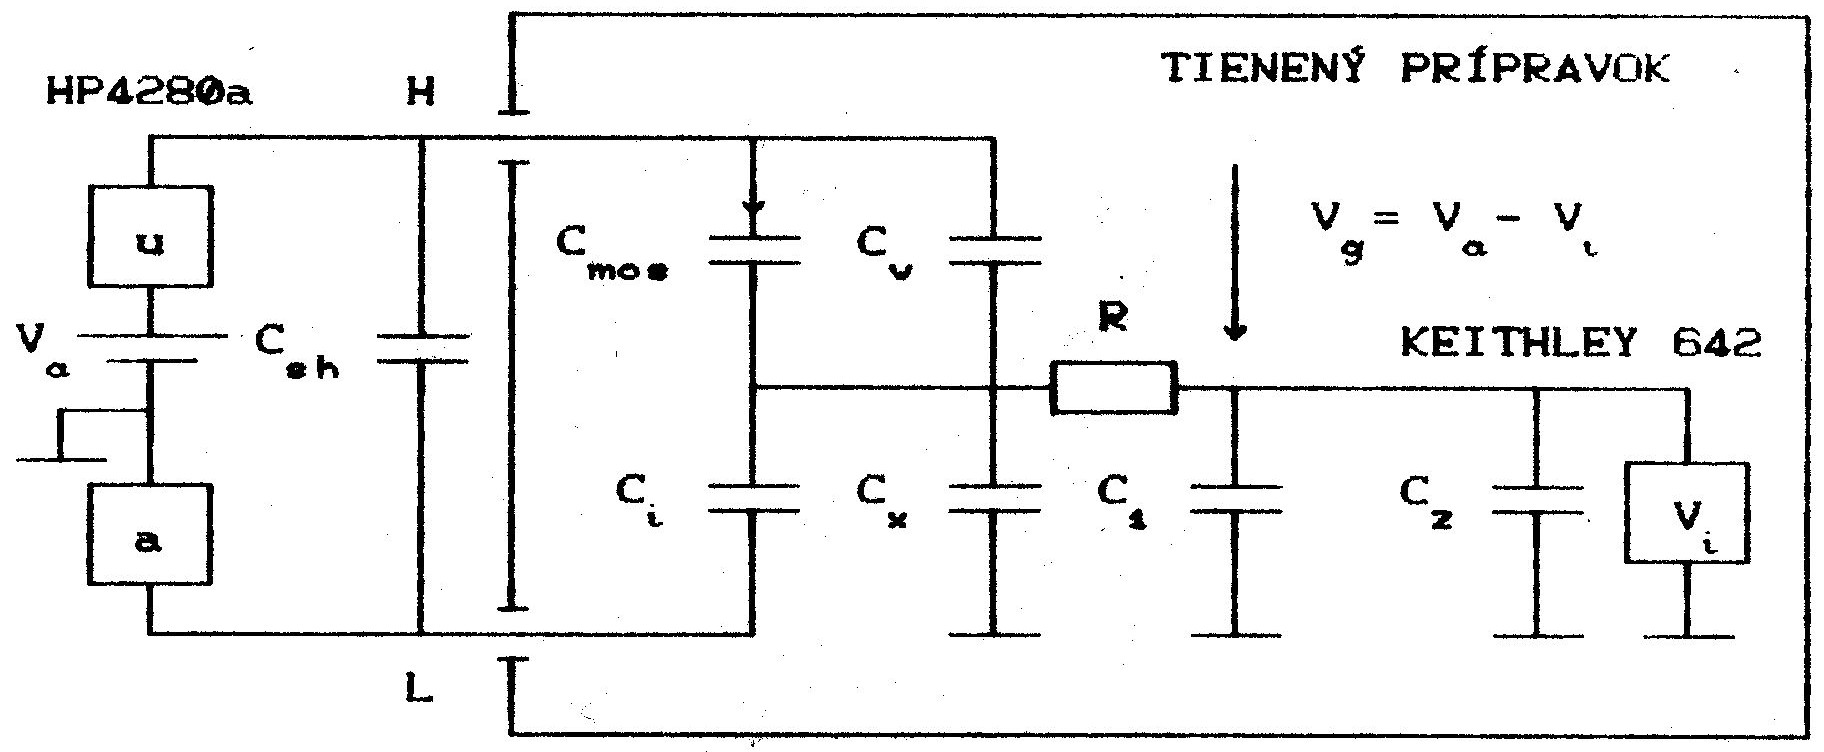
\includegraphics{Figures/fig-app-1.eps}
  \caption[Engagement Q-C method implemented on KME EF
    STU.]{Connection Q-C method implemented at KME EF
    STU.}\label{fig:App.1}
\end{figure}

\par Figure~\ref{fig:App.1} shows the detailed wiring of the workbench
and the measuring instruments of the Q-C method. In the left part of
the figure is shown the measuring instrument HP4280a, which in our
diagram consists of a DC voltage source $V_a$, which is used to
measure structure is brought to the desired state, a source of
high-frequency signal (denoted by u) and an ammeter (denoted by a).
Capacitance $C_{sh}$ represents the parasitic capacitance of the lead
wires, which can be can be eliminated directly by the HP4280a meter
and is therefore will not be considered further. $C_{mos}$ is the
capacitance of the measured structure and $C_i$ represents the
voltage-independent capacitor. Capacitance $C_w$ represents the
parasitic capacitance between the table on which the the structure to
be measured and the raised tip of the probe. $C_x$ indicates the
parasitic capacitance between the common point of connection of the
capacitors (hereafter referred to as common point) and ground. $C_1$
represents the parasitic capacitance of the lead wire to the voltmeter
and $C_2$ indicates the input capacitance of the voltmeter.  These
capacitances $C_1$ and $C_2$ together with the resistance R a low-pass
filter that isolates the voltmeter from the high-frequency signal
generated by the HP4280a. The problem of high frequency measurement is
the fact that the ammeter of the instrument HP4280a does not measure
the component of current flowing from a common point through
capacitors $C_x$, $C_1$ and $C_2$ to ground. This fact should be
should be taken into account when evaluating the high-frequency
measurement. For the final evaluation of the measured data, the
following problems need to be solved:

\begin{itemize}
\item determine the capacitance of $C_i$
\item determination of the parasitic capacitance $C_w$
\item determine the parasitic capacitance $Cx$
\item determine the capacitance of $C_{iLF}  = C_i + C_1 + C_2$
\item correction of the measured high frequency capacitance $C_m$ with respect to
  the current flowing through $C_x + C_1 + C_2$ to ground.
\end{itemize}


\section{Determining the parasitic capacity of $C_w$.}\label{sec:E.1}

A detailed description of the methodology for measuring the parasitic
capacitance $C_w$ is given in the Appendix
2.\ literature~\cite{App.2}. In our experiment, we mentioned
methodology was modified in a way that led to a greater
reproducibility of the results. We describe this procedure.

\begin{enumerate}

\item We connect the MOS structure and at $V_a = 0$ momentarily ground
  the common point to ensure zero external charge on the capacitors.

\item With voltage $V_a$ bring the MOS structure to accumulation and
  read the values $V_a = V_{a0}$ and $V_i = V_{i0}$.

\item Bring the MOS structure into accumulation with a higher voltage
  $V_a$ and read the values $V_a = V_{a1}$ and $V_i = V_{i1}$. From the
  conservation law of charge follows
  \begin{equation}\label{eq:E.1}
  (C_{ox} + C_w)(V_{g1} - V_{g0}) = (C_{iLF} + C_x)(V_{i1} - V_{i0})
  \end{equation}

\item Set $V_a=0$, momentarily ground the common point and pick up the
  probe tip just enough to break contact.

\item Set $V_a \neq 0$ and read $V_a = V_{a2}$ and  $V_i = V_{i2}$.

\item Increase the voltage $V_a$ and subtract the values $V_a =
  V_{a3}$ a $V_i = V_{i3}$. The law of conservation of charge implies
  \begin{equation}\label{eq:E.2}
    C_w(V_{g3} - V_{g2}) = (C_{iLF} + C_x)(V_{i3} - V_{i2})
  \end{equation}

\item By comparing the equations~\ref{eq:E.1} and~\ref{eq:E.2}, we
  obtain the expression to calculate the capacity of $C_w$, which can
  be evaluated, assuming, that we know the capacity of the oxide layer
  of the MOS structure.
  \begin{equation}\label{eq:E.3}
    C_w = C_{ox} \cfrac{1} {\cfrac{\cfrac{V_{g3}-V_{g2}}{V_{g1}-V_{g0}}} {\cfrac{V_{i3}-V_{i2}}{V_{i1}-V_{i0}}} -1}
  \end{equation}

\end{enumerate}

\section{Determining the parasitic capacity of $C_x$.}\label{sec:E.2}

See Appendix 10.\ of the literature~\cite{App.4} for a description of
the direct measurement of the parasitic capacitance of $C_x$. However,
the experimental results show that this measurement is subject to a
large error and its reproducibility is small. Therefore, we have
chosen in our experiment procedure, the principle of which is outlined
in the Appendix 5.\ of the literature~\cite{App.4}. As can be seen in
Appendix~\ref{sec:E.4}, the high-frequency capacitance of the MOS
$C_{mos}$ structure is a function of of the parasitic capacitance
$C_x$ that we wish to determine. In accumulation, the $C_{mos} =
C_{ox}$, which can be achieved by a suitable variation of of $C_x$. In
our evaluation of the data measured by the Q-C method, we variation of
$C_x$, we used the interval division method.

\section{Capacity determination $C_{iLF}$.}\label{sec:E.3}

In Appendix 10.\ of the literature~\cite{App.4} is a description of
the direct measurement of the parasitic capacitance
$C_{iLF}$. However, similar to the measurement of $C_x$, the
experimental results show that this measurement is loaded by a large
error. Therefore, we have chosen a procedure based on the condition,
that the low and high frequency capacitances of the MOS structure must
have the same value in accumulation. The determination of $C_{iLF}$ is
then based on the following relation

\begin{equation}\label{eq:E.4}
  \frac{\delta}{\delta C_{iLF}} \sum\limits_{j} {\Big[C_{mos}^{LF}(j) - C_{mos}^{HF}(j)\Big]}^2 = 0
\end{equation}

, where the above summation is performed for points measured in
accumulation. A description of the derivation of the relation for the
calculation of $C_{iLF}$ is given in the Appendix 4.\ of the
literature~\cite{App.4} and here we only give its final form.

\begin{equation}\label{eq:E.5}
  C_{iLF} = \frac{\sum\limits_{j}{\Bigg[C_{mos}^{HF}(j)+C_{w}\Bigg]}{\Bigg[\cfrac{dV_i}{dV_g}\Bigg]}_j}{\sum\limits_{j}{\Bigg[\cfrac{dV_i}{dV_g}\Bigg]}_j}
\end{equation}

It should be noted that the above procedure has the advantage that its
use guarantees the coincidence of low and high frequency capacitance
dependence of the MOS structure in the accumulation, which constitutes
a good basis for calculation of the interface traps from the two
capacitance dependencies mentioned above.

\section{High frequency capacitance correction $C_m$.}\label{sec:E.4}

In Appendix 1.\ of the literature~\cite{App.2} an analysis of the Q-C
method from a high-frequency measurement perspective. Here we give its
main idea.

\begin{figure}[h!]\centering
  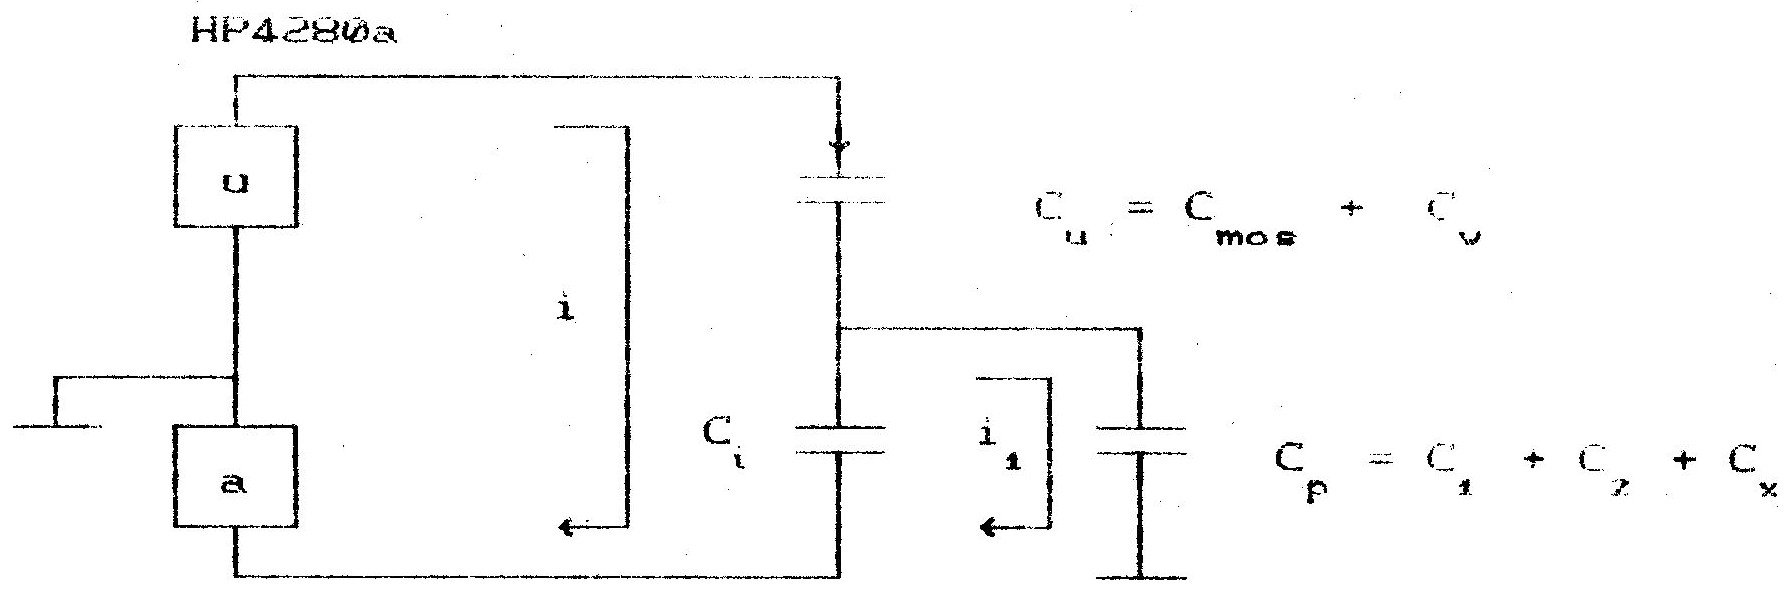
\includegraphics{Figures/fig-app-2.eps}
  \caption[Equivalent wiring of the Q-C method for high-frequency
    measurements]{Equivalent wiring of the Q-C method for
    high-frequency measurement.}\label{fig:App.2}
\end{figure}

As can be seen from the figure~\ref{fig:App.2} ammeter of the HP4280a
instrument does not measure the current $i_1$ flowing through the
capacitor $C_p$. The capacitance $C_m$, which we measure with this
instrument can be expressed by the relation

\begin{equation}\label{eq:E.6}
  C_m = \frac{C_{u} C_{iHF}} {C_{iHF}+C_{u}+C_{p}}
\end{equation}

Chapter~\ref{sec:3.3} gives the relations for calculating of the
frequency capacity of the MOS\@ structure.  In order for the results
obtained from relations~\ref{eq:3.3} are not affected by the above
fact, it is necessary to to make the following corrections (according
to Appendix 1.\ of the literature~\cite{App.4})

\begin{equation}\label{eq:E.7}
  C_{iHF}=C_{iHF}k, \qquad G_{m}=G_{m}k, \qquad C_{m}=C_{m}k
\end{equation}

, where

\begin{equation}\label{eq:E.8}
  k = 1 + \frac{C_x}{C_{iHF}}
\end{equation}

% Appendix F

\chapter{Calculation of the surface potential $\varphi_s$ from Q-C method.}\label{app:AppendixF}
\lhead{Appendix F. \emph{Calculation of surface potential $\varphi_s$ from Q-C method}}

The method for determining the surface potential of an MOS structure
is described in Appendix~\ref{app:AppendixC}. Here we give its main idea.

To change the charges on a series-parallel circuit of Q-C capacitors
methods we can write (see Appendix~\ref{app:AppendixE}).

\begin{equation}\label{eq:F.1}
  \Delta Q_x + \Delta Q_i = \Delta Q_w + \Delta Q_{mos}
\end{equation}

If we express the change of charge on voltage-independent capacitors
by their capacitance and voltage, assuming that we start from the
state where $V_i=0$ and $V_g=0$, we can write

\begin{equation}\label{eq:F.2}
  \Delta Q_{mos} = (C_{iLF} + C_{x})V_{i} - C_{w}V_{g}
\end{equation}

We can also express the change of charge on the MOS structure by its
own parameters

\begin{equation}\label{eq:F.3}
  \Delta Q_{mos} = C_{ox}(V_{g} - \varphi_{s} + \varphi_{s0})
\end{equation}

and by combining~\ref{eq:F.2} and~\ref{eq:F.3} we can write the
resulting relation

\begin{equation}\label{eq:F.4}
  \varphi_{s} = \varphi_{s0} - \frac{C_{iLF} + C_{x}}{C_{ox}}V_i + {\bigg[1 + \frac{C_{w}}{C_{ox}}\bigg]}V_{g}
\end{equation}

% Appendix G

\chapter{Určenie povrchového potenciálu $\varphi_{s0}$ pri nulovom napätí hradla.} % Main appendix title

\label{app:AppendixG} % For referencing this appendix elsewhere, use \ref{AppendixA}

\lhead{Appendix G. \emph{Určenie povrchového potenciálu $\varphi_{s0}$ pri nulovom napätí hradla}} % This is for the header on each page - perhaps a shortened title

Vo vzťahu \ref{eq:F.4} vystupuje výraz $\varphi_{s0}$, ktorý
predstavuje povrchový potenciál polovodiča štruktúry MOS v prípade, že
na štruktúru MOS nepôsobí žiadne vonkajšie napätie.  Tento potenciál
je spôsobený rozdielom výstupných prác kovu a polovodiča a nábojmi
nachadzájúcimi sa v izolante a na jeho rozhraní s polovodičom. Na
určenie tejto konštanty použijeme porovnanie nameranej a teoretickej
závislosti $\varphi_{s}$ od šírky OPN, ako je uvedené v
\cite{App.3}. Šírku OPN pre experimentálnu závislosť $\varphi_{s}(w)$
určíme zo vzťahu

\begin{equation}\label{eq:G.1}
w = \epsilon \Bigg[\frac{1}{C_{mos}^{HF}} - \frac{1}{C_{ox}}\Bigg]
\end{equation}

Pre určenie teoretickej závislosti $\varphi_{s}(w)$ použijeme
aproximáciu popísanu v \cite{App.5}

\begin{equation}\label{eq:G.2}
\beta \varphi_{s} = \frac{1}{2} \Big[\frac{w}{L_{DE}}\Big]^2 + \frac{1}{N_{B}L_{DE}^{2}} \int_{0}^{w}x[N(x)-N_{B}]dx + 1
\end{equation}

kde $L_{DE}$ je extrinzická Debayova dĺžka, $N_{B}$ koncentrácia
substrátu a $N(x)$ priebeh koncentrácie dotujúcich prímesí v
podpovrchovej oblasti polovodiča. Na obrázku \ref{fig:App.3} je
znázornený priebeh uvedených závislostí pre namerané dáta Q-C metódy z
obrázku \ref{fig:3.4}. Hodnotu $\varphi_{s0}$ potom určíme z rozdielu
experimentálnej a teoretickej závislosti $\varphi_{s}(w)$ v hĺbke w,
ktorá zodpovedá stavu ochudobnenia štruktúry MOS. Ako je uvedené v
\cite{App.3} aproximácia \ref{eq:G.2} ignoruje voľné nosiče náboja, z
čoho vyplýva jej obmedzenie platnosti len pre stav ochudobnenia.
Uvedeným spôsobom možno vypočítať aj integračnú konštantu pri výpočte
závislosti $\varphi_{s}(V_{g})$ pomocou Berglundovho integrálu.

\begin{figure}[h!]\centering
%\framebox[10cm]{\rule{0cm}{3cm}}
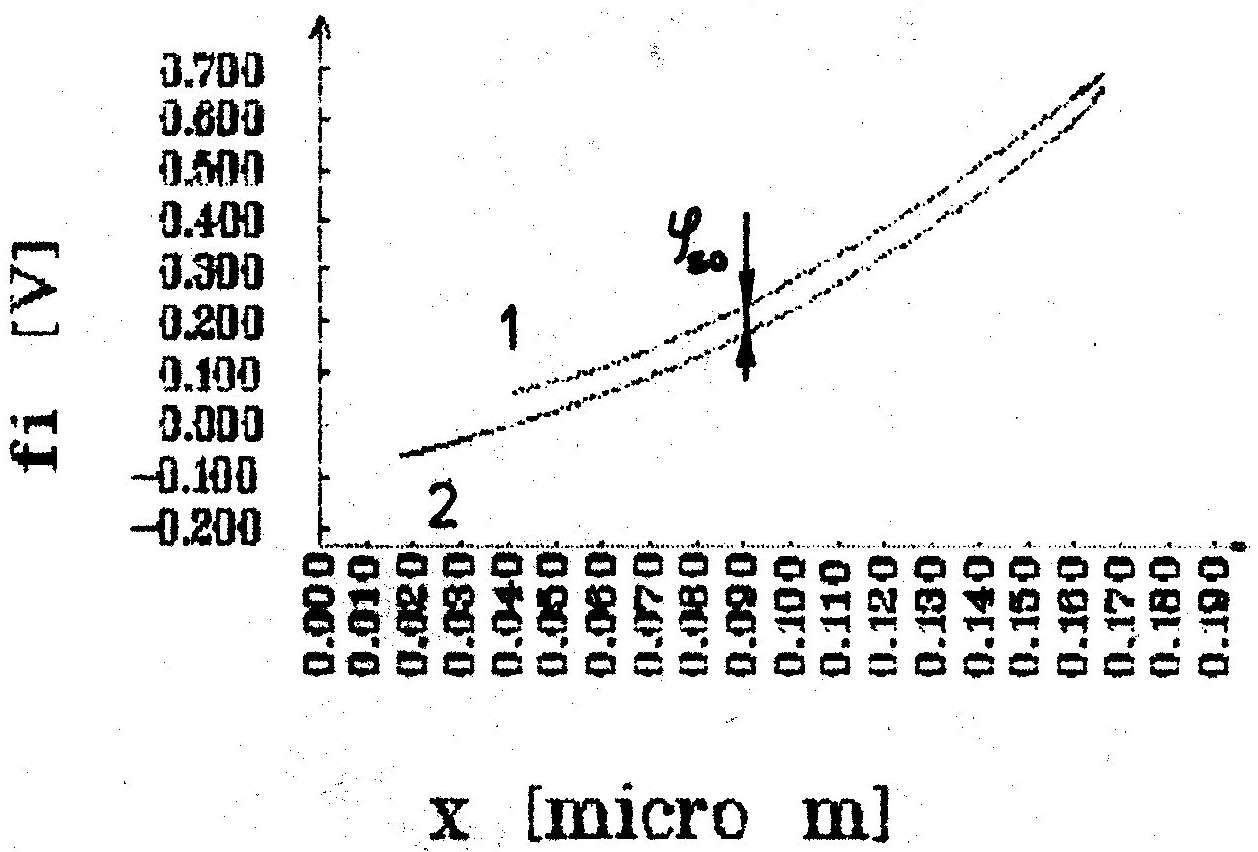
\includegraphics{Figures/fig-app-3.eps}
\captionsetup{justification=raggedright, singlelinecheck=false}
\caption[Priebeh povrchového potenciálu ako závislosti šírky OPN pre
  štruktúru MOS privedenú do stavu hlbokého ochudobnenia]{Priebeh
  povrchového potenciálu ako závislosti šírky OPN pre štruktúru MOS
  privedenú do stavu hlbokého ochudobnenia.  Krivka 1 predstavuje
  priebeh $\varphi(x)$ vypočítaný podľa vztahu \ref{eq:G.2} a krivka 2
  znázorňuje závislosť určenú z experimentálnych dát pomocou vzťahu
  \ref{eq:F.4}.}
\label{fig:App.3}
\end{figure}
% OBR10.BIT

% Appendix H

\chapter{Programs for data acquisition, processing and display for area distribution of MOS structure parameters.}\label{app:AppendixH}
\lhead{Appendix H. \emph{Data acquisition, processing and display programs}}

\begin{verbatim}
I. DATA COLLECTION PROGRAMS.

  All data acquisition programs use a stepper to control the programs
  to control the device:

   * ZONDUP.EXE - table stroke
   * ZONDDN.EXE - table start
   * ZONDST.EXE - table feed

   They read information about the movement of the stepper from the Z.XY subfile

1. ZCT.EXE      - Main program of the CCT method
   Segments:
   * ZCT1.EXE   - initialization of IMS-2 bus and devices
   * ZCT2.EXE   - measurement of V(t) and saving dV/dt to the subfile
   * ZCT9.EXE   - putting the IMS-2 bus into the flood state

2. ZHF.EXE      - Main program of equilibrium and non-equilibrium HF CV method
   Segments:
   * ZHF1.EXE   - initialization of IMS-2 bus and devices
   * ZHF2.EXE   - C(V ) measurement
   * ZHF3.EXE   - smoothing of measured data and saving to a subfile
   * ZHF9.EXE   - setting the IMS-2 bus to the flood state

3. ZLF.EXE      - Main program of quasi-static CV method
   Segments:
   * ZLF1.EXE   - initialization of IMS-2 bus and devices
   * ZLF2.EXE   - measurement of the C(V ) dependence
   * ZLF3.EXE   - smoothing of the measured data, interpolation and saving to a subfile
   * ZLF9.EXE   - putting the IMS-2 bus into a flood state

4. ZOXHF.EXE    - Measurements of the oxide capacity using the HF CV method
   Segments:
   * ZOXHF1.EXE - initialization of IMS-2 bus and instruments
   * ZOXHF2.EXE - oxide layer capacitance measurement and saving to subfile
   * ZOXHF9.EXE - putting the IMS-2 bus into the trigger state

5. ZOXLF.EXE    - Oxide capacitance measurements using quasi-static CV method
   Segments:
   * ZLF1.EXE   - Initialization of IMS-2 bus and instruments
   * ZOXLF2.EXE - oxide layer capacitance measurements and storage in a subfile
   * ZLF9.EXE   - resetting the IMS-2 bus to its original state


II. DATA PROCESSING PROGRAMS.

6.    ZNX.EXE - calculation of concentration profile N(x)
7.    ZNB.EXE - calculation of substrate concentration N
8.    ZFV.EXE - calculation of surface potential as a function of 
                of the gate voltage f (V )
9.    ZDF.EXE - calculation of interface trap density D
10.   ZTX.EXE - calculation of generation time of minority lifetime 
                of charge carriers t (x)
11.  ZWOX.EXE - calculation of the oxide roughness h
12.  ZYXI.EXE - calculation of integral value Y(x)
13.  ZYXM.EXE - calculation of the mean value, standard deviation
                error and linear regression
14.ZKORFF.EXE - calculation of the correlation coefficient between para-
                meters from Subor1 <> Subor2
15.ZKORYX.EXE - calculation of correlation coefficient of dependence Y(x)


III. GRAPHICAL DATA DISPLAY PROGRAMS.

16.   ZGF.EXE - display of the dependence Y(x) with a description of the axis
17. ZSURF.EXE - full screen display of the distribution of parameters and
                functional dependencies Y(x), for different x
18. ZVIEW.EXE - display of individual Y(x) dependencies
19.ZVIEWD.EXE - display of individual Y1(x) and Y2(x) dependencies


IV. AUXILIARY PROGRAMS.

20.   BELL.EXE - alarm
21. ZASCII.EXE - conversion of binary format to ASCII
22. ZERR.EXE   - printout of positions on the board with erroneous measured data
23. ZREPLC.EXE - exchange of records in the data subfile
24. ZTRUNC.EXE - short-circuit of data subfile
\end{verbatim}

% Appendix Bibliography
%\chapter{Literatúra k dodatkom} % Main appendix title
%\label{app:AppendixBibliography} % For referencing this appendix elsewhere, use \ref{AppendixA}
%\lhead{\emph{Literatúra k dodatkom}} % This is for the header on each page - perhaps a shortened title

\begin{thebibliography}{}
\bibitem[App.1]{App.1} El- Sissi H., Cobbold R.S.C. : Electronic Letters 25
  (1973) s.594.
\bibitem[App.2]{App.2} Nicollian E.H., Brews J.R. : Solid St.  Electron. 27
  (1984) s.953.
\bibitem[App.3]{App.3} Brews J.R., Nicollian E.H. : Solid St.  Electron. 27
  (1984) s.963.
\bibitem[App.4]{App.4} Boulin D.M., Brews J.R., Nicollian E.H.  : Solid St.
  Electron. 27 (1984) s.977.
\bibitem[App.5]{App.5}  Brews J.R. : Solid St. Electron. 25 (1982) s.375.
\end{thebibliography}

\addtocontents{toc}{\vspace{2em}} % Add a gap in the Contents, for aesthetics

%----------------------------------------------------------------------------------------
%	INDEX
%----------------------------------------------------------------------------------------
\newpage
\lhead{\emph{Index}} % Change the page header to say "Index"
\addcontentsline{toc}{chapter}{Index}
\printindex
\backmatter

%----------------------------------------------------------------------------------------
%	BIBLIOGRAPHY
%----------------------------------------------------------------------------------------
\label{Bibliography}
\lhead{\emph{Bibliography}} % Change the page header to say "Bibliography"
\bibliographystyle{unsrtnat} % Use the "unsrtnat" BibTeX style for formatting the Bibliography
\bibliography{Bibliography} % The references (bibliography) information are stored in the file named "Bibliography.bib"

\end{document}  
